% Customizable fields and text areas start with % >> below.
% Lines starting with the comment character (%) are normally removed before release outside the collaboration, but not those comments ending lines

\def\WtoLN    {\ensuremath{\mathrm{W}\to\ell\cPgn}}
\def\WtoEN    {\ensuremath{\mathrm{W}\to\Pe\cPgn}}
\def\WtoMN    {\ensuremath{\mathrm{W}\to\Pgm\cPgn}}
\def\ZtoBB    {\ensuremath{\mathrm{Z}\to\bbbar}}
\def\ZtoNN    {\ensuremath{\mathrm{Z}\to\cPgn\bar{\cPgn}}}
\def\ZtoLL    {\ensuremath{\mathrm{Z}\to\ell\ell}}
\def\ZtoMM    {\ensuremath{\mathrm{Z}\to\MM}}
\def\ZtoEE    {\ensuremath{\mathrm{Z}\to\EE}}
\def\WmnJ     {\ensuremath{\mathrm{W}(\Pgm\cPgn)\mathrm{+jets}}}
\def\ZmmJ     {\ensuremath{\mathrm{Z}(\Pgm\Pgm)\mathrm{+jets}}}
\def\ZnnJ     {\ensuremath{\mathrm{Z}(\cPgn\bar{\cPgn})\mathrm{+jets}}}
\def\WJ       {\ensuremath{\mathrm{W + jets}}}
\def\HBB      {\ensuremath{\mathrm{H}\to\bbbar}}
\def\HTT      {\ensuremath{\mathrm{H}\to\TT}}
\def\mtW      {\ensuremath{M_{\mathrm{T}}}}
\def\ptl      {\ensuremath{p_{\mathrm{T}}^{\ell}}}
\def\MyZ      {\ensuremath{\mathrm{Z}}}
\def\MyW      {\ensuremath{\mathrm{W}}}
\def\MyH      {\ensuremath{\mathrm{H}}}
\def\Vudscg   {\ensuremath{\mathrm{V+udscg}}}
\def\Wudscg   {\ensuremath{\mathrm{W+udscg}}}
\def\Wenudscg {\ensuremath{\mathrm{W}(\Pe\cPgn)+\mathrm{udscg}}}
\def\Wmnudscg {\ensuremath{\mathrm{W}(\Pgm\cPgn)+\mathrm{udscg}}}
\def\Wenbb    {\ensuremath{\mathrm{W}(\Pe\cPgn)+\bbbar}}
\def\Wmnbb    {\ensuremath{\mathrm{W}(\Pgm\cPgn)+\bbbar}}
\def\Zeebb    {\ensuremath{\mathrm{Z}(\Pe\Pe)+\bbbar}}
\def\Zmmbb    {\ensuremath{\mathrm{Z}(\Pgm\Pgm)+\bbbar}}
\def\Zudsg    {\ensuremath{\mathrm{Z+udsg}}}
\def\Zudscg   {\ensuremath{\mathrm{Z+udscg}}}
\def\Zeeudscg {\ensuremath{\mathrm{Z}(\Pe\Pe)+\mathrm{udscg}}}
\def\Zmmudscg {\ensuremath{\mathrm{Z}(\Pgm\Pgm)+\mathrm{udscg}}}
\def\Zenbb    {\ensuremath{\mathrm{Z}(\Pe\cPgn)+\bbbar}}
\def\Zmnbb    {\ensuremath{\mathrm{Z}(\Pgm\cPgn)+\bbbar}}
\def\Wbb      {\ensuremath{\mathrm{W\bbbar}}}
\def\Zbb      {\ensuremath{\mathrm{Z\bbbar}}}
\def\Zcc      {\ensuremath{\mathrm{Z\ccbar}}}
\def\Vbb      {\ensuremath{\mathrm{V+\bbbar}}}
\def\Zll      {\ensuremath{Z(\ell\ell)}}
\def\Zmm      {\ensuremath{Z(\mu\mu)}}
\def\Zee      {\ensuremath{Z(ee)}}
\def\Mjj      {\ensuremath{M(\mathrm{jj})}}
\def\ptjj     {\ensuremath{{\pt}(\mathrm{jj})}}
\def\MZ       {\ensuremath{M_{\mathrm{Z}}}}
\def\dRJJ     {\ensuremath{\Delta R(\mathrm{J1,J2})}}
\def\dEtaJJ   {\ensuremath{\Delta \eta(\mathrm{J1,J2})}}
\def\dphiVH   {\ensuremath{\Delta\phi(\mathrm{V,H})}}
\def\dphiWH   {\ensuremath{\Delta\phi(\mathrm{W,H})}}
\def\dphiZH   {\ensuremath{\Delta\phi(\mathrm{Z,H})}}
\def\dphiMJ   {\ensuremath{\Delta\phi(\mathrm{pfMET,J})}}
\def\cosTH    {\ensuremath{\cos{\theta^*}}}
\def\dThPull  {\ensuremath{\Delta\theta_{\mathrm{pull}}}}
\def\ptV      {\ensuremath{p_{\mathrm{T}}(\mathrm{V})}}
\def\ptH      {\ensuremath{p_{\mathrm{T}}(\mathrm{H})}}
\def\ptZ      {\ensuremath{p_{\mathrm{T}}(\mathrm{Z})}}
\def\ptW      {\ensuremath{p_{\mathrm{T}}(\mathrm{W})}}
\def\Naj      {\ensuremath{N_{\mathrm{aj}}}}
\def\Nal      {\ensuremath{N_{\mathrm{al}}}}
\def\etaTF    {\ensuremath{\left | \eta \right | < 2.5}}
\def\Bexp     {\ensuremath{B_{\mathrm{exp}}}}
\def\Bobs     {\ensuremath{B_{\mathrm{obs}}}}
\def\Nobs     {\ensuremath{N_{\mathrm{obs}}}}

% svn info. These are modified by svn at checkout time.
% The last version of these macros found before the maketitle will be the one on the front page,
% so only the main file is tracked.
% Do not edit by hand!
\RCS$Revision: 131141 $
\RCS$HeadURL: svn+ssh://svn.cern.ch/reps/tdr2/notes/AN-12-137/trunk/AN-12-137.tex $
\RCS$Id: AN-12-137.tex 131141 2012-06-20 17:23:42Z srappocc $
%%%%%%%%%%%%% local definitions %%%%%%%%%%%%%%%%%%%%%
% This allows for switching between one column and two column (cms@external) layouts
% The widths should  be modified for your particular figures. You'll need additional copies if you have more than one standard figure size.
\newlength\cmsFigWidth
\ifthenelse{\boolean{cms@external}}{\setlength\cmsFigWidth{0.85\columnwidth}}{\setlength\cmsFigWidth{0.4\textwidth}}
\ifthenelse{\boolean{cms@external}}{\providecommand{\cmsLeft}{top}}{\providecommand{\cmsLeft}{left}}
\ifthenelse{\boolean{cms@external}}{\providecommand{\cmsRight}{bottom}}{\providecommand{\cmsRight}{right}}
%%%%%%%%%%%%%%%  Title page %%%%%%%%%%%%%%%%%%%%%%%%
\cmsNoteHeader{AN-12-137} % This is over-written in the CMS environment: useful as preprint no. for export versions
% >> Title: please make sure that the non-TeX equivalent is in PDFTitle below
\title{Measurement of jet mass in V+Jets events}

% >> Authors
%Author is always "The CMS Collaboration" for PAS and papers, so author, etc, below will be ignored in those cases
%For multiple affiliations, create an address entry for the combination
\address[fnal]{Fermilab}
\address[cern]{CERN}
\address[jhu]{Johns Hopkins University}
\address[davis]{University of California, Davis}
\address[princeton]{Princeton University}


\author[jhu]{Salvatore Rappoccio}
\author[fnal]{Nhan Tran}
\author[fnal]{Kalanand Mishra}
\author[princeton]{David Lopes-Pegna}

%--- Set here, reverse in the PAS:
\newcommand{\ifnpas}{\iftrue}
\newcommand{\ifpas}{\iffalse}

% >> Date
% The date is in yyyy/mm/dd format. Today has been
% redefined to match, but if the date needs to be fixed, please write it in this fashion.
% For papers and PAS, \today is taken as the date the head file (this one) was last modified according to svn: see the RCS Id string above.
% For the final version it is best to "touch" the head file to make sure it has the latest date.
\date{\today}

% >> Abstract
% Abstract processing:
% 1. **DO NOT use \include or \input** to include the abstract: our abstract extractor will not search through other files than this one.
% 2. **DO NOT use %**                  to comment out sections of the abstract: the extractor will still grab those lines (and they won't be comments any longer!).
% 3. **DO NOT use tex macros**         in the abstract: External TeX parsers used on the abstract don't understand them.
\abstract{
A measurement of the jet mass in vector-boson-plus-jets events is presented.
}

% >> PDF Metadata
% Do not comment out the following hypersetup lines (metadata). They will disappear in NODRAFT mode and are needed by CDS.
% Also: make sure that the values of the metadata items are sensible and are in plain text (no TeX! -- for \sqrt{s} use sqrt(s) -- this will show with extra quote marks in the draft version but is okay).

\hypersetup{%
pdfauthor={Andreas Hinzman, Justin Pilot, Michael Mulhearn, Robin
  Erbacher, Salvatore Rappoccio, Nhan Tran, Kalanand Mishra, David Lopes-Pegna},%
pdftitle={Measurement of jet mass in V+Jets events},%
pdfsubject={CMS},%
pdfkeywords={CMS, physics, software, computing}}

\maketitle %maketitle comes after all the front information has been supplied

% >> Text
%%%%%%%%%%%%%%%%%%%%%%%%%%%%%%%%  Begin text %%%%%%%%%%%%%%%%%%%%%%%%%%%%%
%% **DO NOT REMOVE THE BIBLIOGRAPHY** which is located before the appendix.
%% You can take the text between here and the bibiliography as an example which you should replace with the actual text of your document.
%% If you include other TeX files, be sure to use "\input{filename}" rather than "\input filename".
%% The latter works for you, but our parser looks for the braces and will break when uploading the document.
%%%%%%%%%%%%%%%
\section{Introduction}
\section{Introduction}
\label{sec:intro}
% ---- ---- ---- ---- ---- ---- ---- ---- ---- ---- ---- ---- ---- ---- ---- ---- ---- ---- ---- ---- ---- ---- ----

The Standard Model (SM) of particle physics successfully describes the majority of high-energy
experimental data~\cite{pdg}. One of the key remaining questions is the origin of the masses of
W and Z bosons.  In the simplest implementation of the SM, it is attributed to the spontaneous
breaking of electroweak symmetry caused by a new scalar field. %~\cite{Higgs1, Higgs2, Higgs3} 
The existence of the associated field quantum, the Higgs boson, has yet to be experimentally confirmed.
Therefore, the search for the Higgs boson is arguably one of the most
important studies being done at the LHC~\cite{lhcmachine}. For Higgs
masses above or near the threshold for decay into two vector bosons,
the decay modes of choice are dominated by those decays because of
their large branching fractions.
It is clear that the events where one $W$ decays leptonically, which
provides the main trigger elements, while the other decays
hadronically have the second highest branching fraction and have a
reconstructable Higgs mass peak~\cite{intro2}. 

This note contains the analysis that sets a limit on the Higgs boson cross-section
based on this decay mode, 
performed on the 2012 data acquired by CMS at $\sqrt{s}~=$~8~TeV,
following the same procedures applied for the analysis of 2011 data \cite{HIG-12-003}.
The analysis selects events with one well identified and isolated lepton, 
large missing transverse energy and at least two high \pt jets.
Therefore, the main experimental issue is to control the large $W$ plus jets 
background sufficiently well that the advantages of using this 
final state are realized.

With respect to the 2011 analysis, 
the available sample is acquired this year by single lepton triggers, 
allowing to relax the selection on the tranverse mass of the leptonic W boson.
Physics objects are selected with the techniques available in 2012, 
in particular jet identification is applied to reduce the effect of pile-up.
% The likelihood based analysis applies a b-veto on the third jet, 
% in the case of three jets events, 
% while the fit-based analysis is being implemented after a selection on the most discriminating variables
% of the likelihood training.
The theoretical description of the Higgs lineshape 
follows the recommendation from the Higgs Cross Section Working Group \cite{Dittmaier:2012vm},
therefore the theoretical error has additional components related to the exclusive
segregation of events into separate jet bins.

The note is structured as follows. 
A discussion about the data samples used in the analysis and the trigger selections
is presented in Sections~\ref{sec:MCexpectations} and \ref{sec:technicalities}.  
The physics objects reconstruction is discussed in Section~\ref{sec:firstStep}.
The lepton selection and other preselection requirements are described in detail 
in Section~\ref{sec:firstStep} and \ref{sec:dataMCcomparisons}.

%% A first limit extraction is performed with a few set of selections applied on top of these,
%% as described in Section~\ref{sec:firstExtraction}.
%% To enhance the exclusion power of this analysis, 
%% tighter selections are put in place.

After the preselections,
the signal-over-background ratio is enhanced by means of a selection on a MVA discriminant, 
designed in order to control the background while preserving as much as possible the difference in shape
with respect to the signal (Section~\ref{sec:mvaoptimization}).
The input variables of the MVA exploit the decay angles of the four-body mass system, 
the kinematics of the entire four-body system. For high mass points, a quark-gluon discriminating
variable, already exploited in the CMS search for a Standard Model Higgs boson in its $\ell{}\ell{}jj$ decay,
is also used in parallel with the MVA discriminant.
The MVA variable definition is optimized with dedicated trainings for each Higgs mass hypothesis case, 
for each lepton flavour ($e$, $\mu$) and for each jets multiplicity (2 jets, 3 jets) independently.
In this way, 48 different configurations are obtained.

The main background contaminating the signal region is W+jets.
Its $m_{\ell{}\nu{}jj}$ shape is extrapolated from sidebands in the $m_{jj}$ distribution 
through Monte Carlo based factors (Section~\ref{sec:wjetsBackground}).
Also the QCD shapes come from a data-driven determination, as described in Section~\ref{sec:dataDrivenQCD}.
The remaining background shapes come from the Monte Carlo.
The normalization of the backgrounds in the signal region 
is measured by fitting their Monte Carlo shapes on the same sidebands in the $m_{jj}$ variable 
(Section~\ref{sec:mjjfitfornormal}).
The determination of the $m_{jj}$ distribution for W+jets is described in Section~\ref{sec:wjetsShape}.

The systematic uncertainties present in the signal description are described in Section~\ref{sec:systematics}.
Section~\ref{sec:limitExtraction} describes the obtained limits on the Standard Model Higgs cross section
and Section~\ref{sec:conclusions} closes this work.



\ifnpas
\section{CMS Detector}
\fi


\label{sec:cms_detector}


The CMS detector~\cite{:2008zzk}
is a general-purpose device, however it has
many features particularly suited for reconstruction of 
energetic jets,specifically, the finely segmented electromagnetic
and hadronic calorimeters, and the charged particle tracking.
The charged particles are reconstructed by the inner tracker,
immersed in a $3.8$~T axial magnetic field; the inner tracker consists
of three layers and two endcap disks of pixel sensors, and ten
barrel layers and twelve endcap disks of silicon strips.  This
arrangement results
in a full azimuthal coverage within $|\eta| < 2.5$, where $\eta$
is the pseudorapidity and is defined as $\eta = -\ln\tan(\theta/2)$.
The CMS uses a polar coordinate system, with the 
$z$ axis coinciding with the axis of symmetry of the CMS detector,
and oriented in the counterclockwise proton direction; here $\theta$ 
is the polar angle defined with respect to the positive $z$ axis.
The pseudorapidity is an approximation for the full rapidity $y$, and
the approximation is exact for massless particles. Since many of the
particles we use are not massless, we use the full rapidity $y$ which
is defined as $y = \frac{1}{2} \frac {E + p_{z}/c}{E - p_{z}/c}$.

A lead-tungstate crystal electromagnetic calorimeter (ECAL) and 
a brass-scintillator hadronic calorimeter (HCAL) surround the tracking
volume and allow photon, electron and jet reconstruction up to $|\eta|=3$.
The ECAL and HCAL cells are grouped into towers projecting radially 
outward from the interaction region.  In the central region ($|\eta|<1.74$)
the towers have dimensions $\Delta\eta = \Delta\phi = 0.087$; however,
at higher $\eta$, the $\Delta\eta$ and $\Delta\phi$ widths increase.  
ECAL and HCAL
cell energies above the noise suppression thresholds are combined within
each tower to define the calorimeter tower energy, and the towers are further
combined into clusters, which are then identified as jets.  For an improved
jet reconstruction, the tracking and calorimeter information is combined 
in an algorithm called particle-flow~\cite{particleflow}, which is described
below.



\section{Data and trigger}
Table~\ref{tab:datasets} summarizes the data samples used in the current analysis, 
the channels in which they are used, and the approximate luminosity as reported in 
the particular {\tt JSON} file used in each analysis.  
Tables~\ref{tab:SigMC}--\ref{tab:ttbarMC} summarize the simulated samples and their 
equivalent luminosities.  {\tt Fall11} samples are used consistently for all the analysis steps.
 Appropriate pile-up reweighting is 
applied when comparing to data, in order to represent the true primary vertex 
distribution in the different run ranges.  An example of the effect of reweighting
is shown in Fig.~\ref{fig:PVreweight}, which shows the distribution of the number of
primary vertices in data and reweight {\tt Fall11} simulation for a sample of Z$(\mu\mu)$ +jet events
selected as described in Sec.~\ref{sec:Vselection}.  The samples were analyzed with CMSSW 
version 4.2.x and processed through the standard PAT configuration.

\begin{figure}[htbp]
\begin{center}
\subfigure{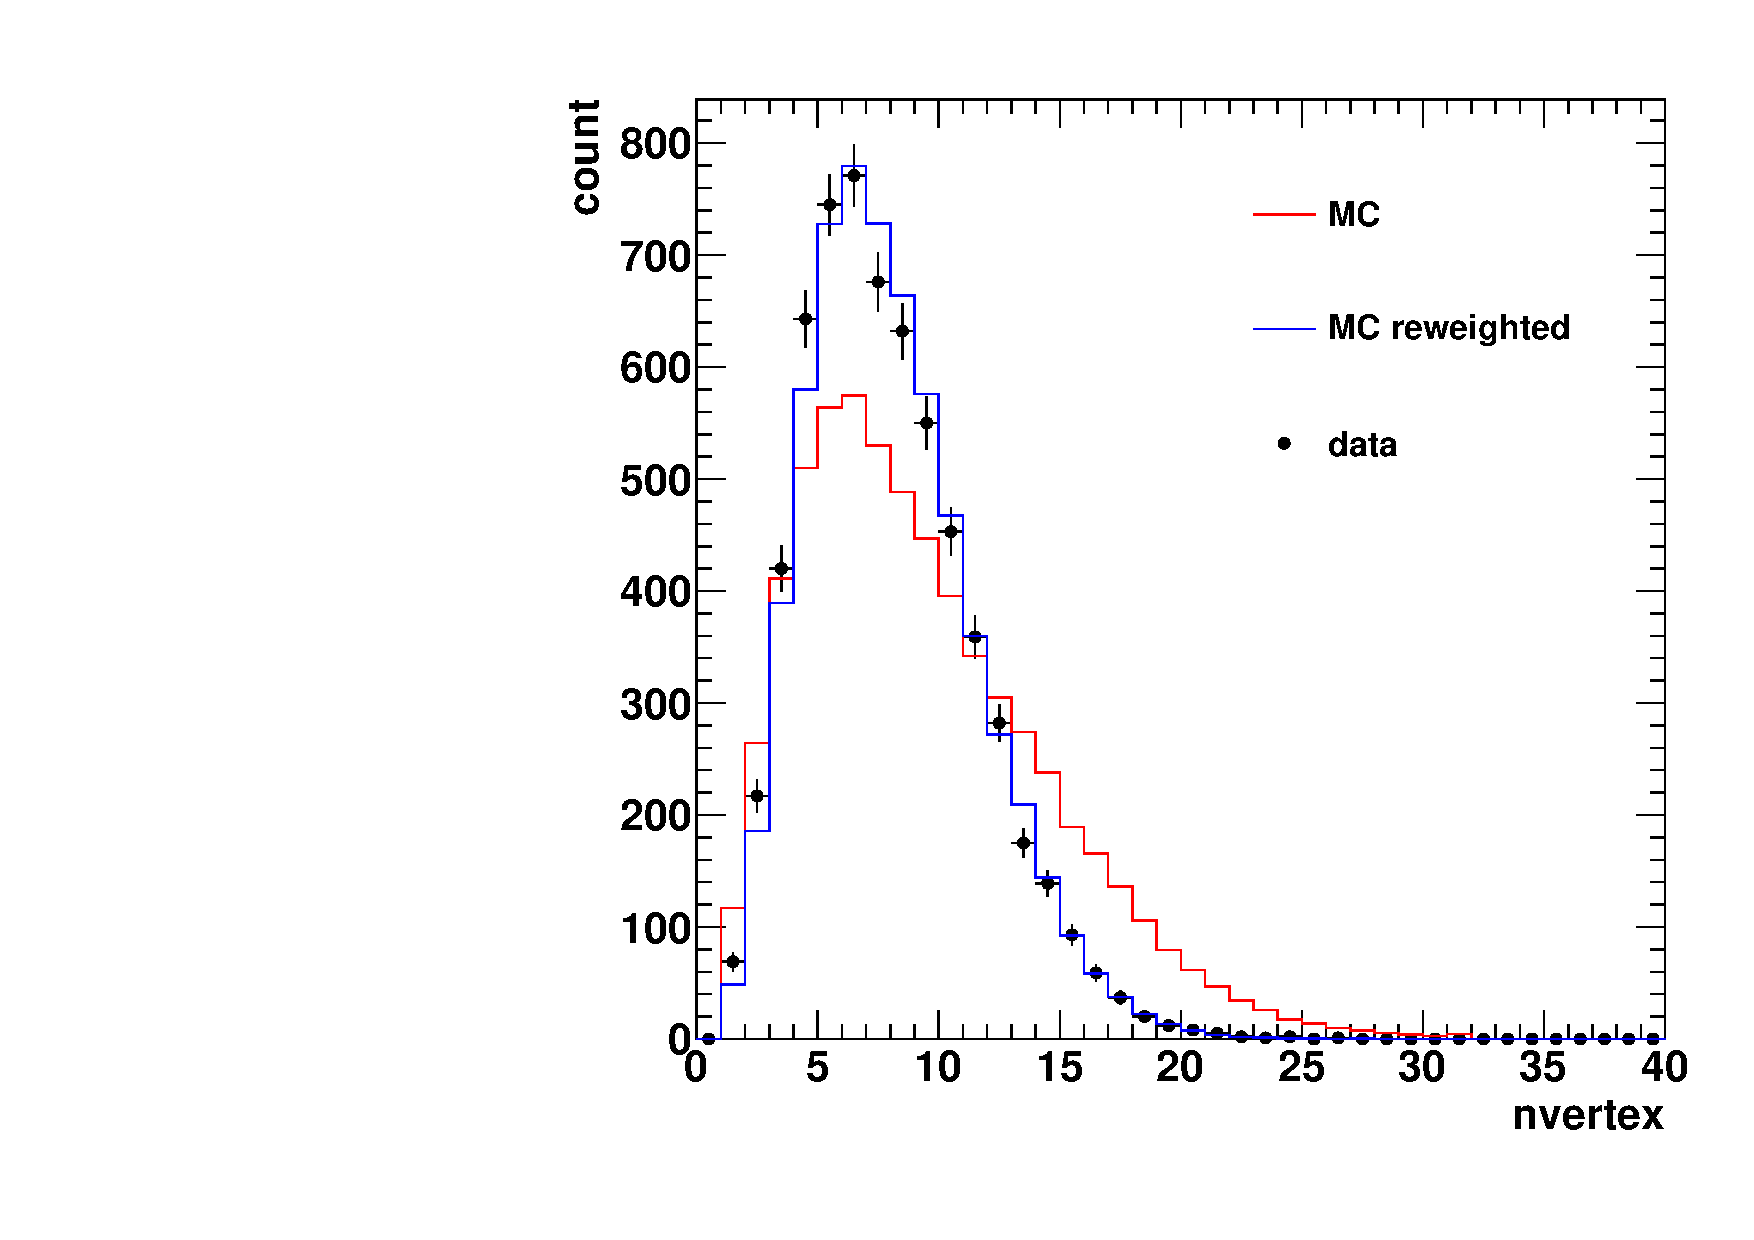
\includegraphics[width=0.49\textwidth]{figs/n_vertices.pdf}}
%    \includegraphics[width=0.48\textwidth]{figures/WmnH-ttbar-nPV-lin}
%    \includegraphics[width=0.48\textwidth]{figures/WmnH-ttbar-nPV-log}
    \caption{Distribution of the number of reconstructed primary vertices in
    data compared to simulation in a sample of Z$(\mu\mu)$+jet events   
    selected as discussed in Sec.~\ref{sec:Vselection} }
    \label{fig:PVreweight}
  \end{center}
\end{figure}

\begin{table}[tbp]
\caption{List of 2011 data samples used for this analysis.  The sum includes approximately
$5. \fbinv$ across all modes.}
\label{tab:datasets}
\begin{center}
\begin{tabular}{ccc} \hline\hline
        Mode                    & Dataset                                           & $\cal L$ (\fbinv) \\\hline
W$(\Pgm\cPgn)$, Z$(\Pgm\Pgm)$ & {\tt /SingleMu/Run2011/May10ReReco}	            & $0.2110$ \\
                                & {\tt /SingleMu/Run2011A/Aug05ReReco}	            & $0.3953$ \\
                                & {\tt /SingleMu/Run2011A/PromptRecoV4}	            & $0.9547$ \\
                                & {\tt /SingleMu/Run2011A/PromptRecoV6}	            & $0.7067$ \\
                                & {\tt /SingleMu/Run2011B/PromptRecoV1}	            & $2.707$ \\
\hline
				& Total Lumi                                        & $4.9748$ \\\hline\hline
W$(\Pe\cPgn)$                  & {\tt /SingleElectron/Run2011/May10ReReco}         &  $0.2156$ \\
                                & {\tt /ElectronHad/Run2011A/Aug05ReReco}           & $0.3953$ \\
                                & {\tt /ElectronHad/Run2011A/PromptRecoV4}          & $0.9553$ \\
                                & {\tt /ElectronHad/Run2011A/PromptRecoV6}          & $0.7067$ \\
                                & {\tt /ElectronHad/Run2011B/PromptRecoV1}          & $2.709$ \\
\hline
				& Total Lumi                                        & $4.6754$ \\\hline\hline
Z$(\Pe\Pe)$                    & {\tt /DoubleElectron/Run2011/May10ReReco}	    & $0.2155$ \\
                                & {\tt /DoubleElectron/Run2011A/Aug05ReReco} 	    & $0.3953$ \\
                                & {\tt /DoubleElectron/Run2011A/PromptRecoV4}       & $0.9553$ \\
                                & {\tt /DoubleElectron/Run2011A/PromptRecoV6}       & $0.7067$ \\
                                & {\tt /DoubleElectron/Run2011B/PromptRecoV1}       & $2.709$ \\
\hline
				& Total Lumi                                        & $4.9818$ \\\hline\hline
\hline\hline
\end{tabular}
\end{center}
\end{table}

\begin{table}[tbp]
\caption{List of diboson {\tt Fall11} Monte Carlo samples used in this version of the note.}
\label{tab:SigMC}
\begin{center}
\begin{tabular}{ccc} \hline\hline
        Mode          & Dataset				       & $\cal L\,(\fbinv)$ \\ \hline
{\small ZZ		      } & {\small  {\tt /ZZtoAnything\_TuneZ2\_7TeV-pythia6-tauola  }}	     & {\small $  675.912 $ } \\
{\small WW		      } & {\small  {\tt /WWtoAnything\_TuneZ2\_7TeV-pythia6-tauola  }}	     & {\small $  98.38 $ } \\
{\small WZ		      } & {\small  {\tt /WZtoAnything\_TuneZ2\_7TeV-pythia6-tauola  }}	     & {\small $  234.35$ } \\
\hline\hline
\end{tabular}
\end{center}
\end{table}

\begin{table}[tbp]
\caption{List of V+jets {\tt Fall11} Monte Carlo samples used in this version of the note.}
\label{tab:VjetsMC}
\begin{center}
\begin{tabular}{ccc} \hline\hline
% update of lumi values for Vjets
        Mode          & Dataset				       & $\cal L\,(\fbinv)$ \\ \hline
%{\tiny W+jets  			} & {\tiny  {\tt /WjetsToLNu\_TuneZ2\_7TeV-madgraph-tauola }}	           & {\tiny $  2.598   $ } \\
{\small W+jets $(\pt >100\GeV)$   	} & {\small  {\tt /WjetsToLNu\_pt100\_7TeV-madgraph-tauola }}	           & {\small $  32.02 $ } \\
{\small W+jets $(\pt >100\GeV)$          } & {\small {\tt /WjetsToLNu\_pt100\_7TeV-herwigpp }}              & {\small $  86.99 $ } \\
%{/tiny Z$\to\ell\ell(M_{\ell\ell}>50)$ } & {\tiny  {\tt /DYJetsToLL\_TuneZ2\_M-50\_7TeV-madgraph-tauola }} & {\tiny $  11.51   $ } \\
{\small Z$\to\ell\ell(\pt > 100\GeV)$ }   & {\small  {\tt /DYJetsToLL\_pt100\_7TeV-madgraph-tauola }}        & {\small $  33.8 $ } \\
{\small Z$\to\cPgn\ell(\pt > 100\GeV)$ }  & {\small  {\tt /DYJetsToLL\_Pt-100\_7TeV-herwigpp }}             & {\small $  81.8 $ } \\
\hline\hline
\end{tabular}
\end{center}
\end{table}

\begin{table}[tbp]
\caption{List of \ttbar\ and single top, and QCD {\tt Fall11} samples used in this analysis.
}
\label{tab:ttbarMC}
\begin{center}
\begin{tabular}{ccc} \hline\hline
        Mode          & Dataset				       & $\cal L\,(\fbinv)$ \\ \hline
{\tiny \ttbar\ 	 } & {\tiny {\tt /TTJets\_TuneZ2\_7TeV-madgraph-tauola/11-PU\_S6\_START42\_V14-v2/AODSIM             }}         & {\tiny $360.$ } \\
{\tiny Single Top (tW)	 } & {\tiny {\tt /T\_TuneZ2\_tW-channel-DR\_7TeV-powheg-tauola/11-PU\_S6\_START42B\_V14-v1/AODSIM     }} & {\tiny $103.5$ } \\
                           & {\tiny {\tt /Tbar\_TuneZ2\_tW-channel-DR\_7TeV-powheg-tauola/11-PU\_S6\_START42B\_V14-v1/AODSIM  }} & {\tiny $102.9$ } \\
{\tiny Single Top (t-ch)} & {\tiny {\tt /T\_TuneZ2\_t-channel\_7TeV-powheg-tauola/11-PU\_S6\_START42B\_V14-v1/AODSIM         }}  & {\tiny $93.0$  } \\
                           & {\tiny {\tt /Tbar\_TuneZ2\_t-channel\_7TeV-powheg-tauola/11-PU\_S6\_START42B\_V14-v1/AODSIM      }} & {\tiny $85.9$  } \\
{\tiny Single Top (s-ch)} & {\tiny {\tt /T\_TuneZ2\_s-channel\_7TeV-powheg-tauola/11-PU\_S6\_START42B\_V14-v1/AODSIM         }}  & {\tiny $81.5$  } \\
                           & {\tiny {\tt /Tbar\_TuneZ2\_s-channel\_7TeV-powheg-tauola/11-PU\_S6\_START42B\_V14-v1/AODSIM      }} & {\tiny $95.8$  } \\
%{\tiny QCD(muon)	 } & {\tiny {\tt /QCD\_Pt-20\_MuEnrichedPt-15\_TuneZ2\_7TeV-pythia6/11-PU\_S6\_START42B\_V14-v2/AODSIM}} & {\tiny $0.296$ } \\
%{\tiny QCD(electron)	 } & {\tiny {\tt /QCD\_Pt-80to120\_TuneZ2\_7TeV\_pythia6/11-PU\_S\_START42\_V11-v1/AODSIM  }}	      & {\tiny $0.008$ } \\
%{\tiny QCD(electron)	 } & {\tiny {\tt /QCD\_Pt-120to170\_TuneZ2\_7TeV\_pythia6/11-PU\_S\_START42\_V11-v1/AODSIM }}	      & {\tiny $0.053$ } \\
%{\tiny QCD(electron)	 } & {\tiny {\tt /QCD\_Pt-170to300\_TuneZ2\_7TeV\_pythia6/11-PU\_S\_START42\_V11-v1/AODSIM }}	      & {\tiny $0.256$ } \\
%{\tiny QCD(electron)	 } & {\tiny {\tt /QCD\_Pt-300to470\_TuneZ2\_7TeV\_pythia6/11-PU\_S\_START42\_V11-v1/AODSIM }}	      & {\tiny $5.500$ } \\
%{\tiny QCD(electron)	 } & {\tiny {\tt /QCD\_Pt-470to600\_TuneZ2\_7TeV\_pythia6/11-PU\_S\_START42\_V11-v1/AODSIM }}	      & {\tiny $56.8$  } \\
\hline\hline
\end{tabular}
\end{center}
\end{table}


A mix of different triggers are used to collect events consistent with
the $V$+jet finsl state signature, in some cases varying
significantly across the 2011 dataset. 

For the $W(\mu\nu)$ and $Z(\mu\mu)$ + jet analyses, we use the logical OR of isolated and non-isolated single muon triggers, with variable thresholds as reported below. For the $W(e\nu)$ + jet analysis, we use the logical OR of single electron triggers, where in addition to a tight isolated electron (with variable momentum threshold), we require a 50 GeV cut on the electron plus PFMET transverse mass.     

\subsection{Single Lepton Triggers}

\subsubsection{Run2011A: Menus 5E32 (Runs: 160404--163869), 
1E33 (Runs:165088--166967), and 1.4E33 (Runs:167039--167913)}
\begin{itemize}
\item
Muon data:\\
     IsoMu17\_v* OR Mu30\_v* \\
Note: We really needed to OR in the nonisolated muon 
trigger as it recovers about half of the offline-isolated 
muons rejected by IsoMu, increasing the trigger efficiency 
by ~5\%. 
\item
Electron data:\\   
Ele27\_CaloIdVT\_CaloIsoT\_TrkIdT\_TrkIsoT\_v* \, \, \, \textcolor{red}{5E32 epoch}\\
Ele25\_WP80\_PFMT40\_v1 \, \, \, \textcolor{red}{1E33 epoch}\\
Ele27\_WP80\_PFMT50\_v* \, \, \, \textcolor{red}{1.4E33 epoch}
\end{itemize}
%%%%%%%%%%%%%%%%%%%%%%%%%%%%%%%
%%%%%%%%%%%%%%%%%%%%%%%%%%%%%%%
\subsubsection{Run2011A:Menu 2E33, Runs 170249--173198}
\begin{itemize}
\item
Muon data:\\
     (IsoMu17\_v13 OR IsoMu20\_v8 OR IsoMu24\_v8) \, \, OR \, \, (Mu30\_v7 OR Mu40\_v5)\\

Note: This epoch was complicated because Mu30, IsoMu17, 
and IsoMu20 were all prescaled for brief periods, so we 
could either break it down into sub-epochs or lump them 
together. We chose the latter because it is predominantly 
IsoMu17 and the sub-epoch lumi accounting is painful.   
\item
Electron data:\\   
Ele27\_WP80\_PFMT50\_v*
\end{itemize}
%%%%%%%%%%%%%%%%%%%%%%%%%%%%%%%
%%%%%%%%%%%%%%%%%%%%%%%%%%%%%%%
\subsubsection{Run2011A:Menu 3E33, Runs: 173236--173692}
\begin{itemize}
\item
Muon data:\\
HLT\_IsoMu20\_v9 OR HLT\_Mu40\_eta2p1\_v1
\item
Electron data:\\
 Ele27\_WP80\_PFMT50\_v*
\end{itemize}
%%%%%%%%%%%%%%%%%%%%%%%%%%%%%%%
%%%%%%%%%%%%%%%%%%%%%%%%%%%%%%%
\subsubsection{Run2011B: Menu 3E33, Runs: 175832--178380}
\begin{itemize}
\item
Muon data:\\
    (IsoMu30\_eta2p1\_v3  OR IsoMu24\_eta2p1\_v3  OR IsoMu24\_v9 OR IsoMu20\_v9) \\
     OR \\  
    (Mu40\_eta2p1\_v1  OR  HLT\_Mu40\_v6)
\item
Electron data:\\  
Ele27\_WP80\_PFMT50\_v* OR Ele27\_WP70\_PFMT50\_v*
\end{itemize}
%%%%%%%%%%%%%%%%%%%%%%%%%%%%%%%
%%%%%%%%%%%%%%%%%%%%%%%%%%%%%%%
\subsubsection{Run2011B: Menu 5E33, Runs: 178420--180252}
\begin{itemize}
\item
Muon data:\\
       (IsoMu30\_eta2p1\_v6 OR IsoMu24\_eta2p1\_v6 OR IsoMu24\_v12 OR \\
       IsoMu30\_eta2p1\_v7 OR IsoMu24\_eta2p1\_v7 OR IsoMu24\_v13) \\
       OR \\
      (Mu40\_eta2p1\_v4 OR  Mu40\_v9) \, \, \,
      \textcolor{red}{(v1.4, 178420-179889)} \\
       OR (Mu40\_eta2p1\_v5 OR  Mu40\_v10) \, \, \,
      \textcolor{red}{(v2.2, 179959--180252)}
\item
Electron data:\\
 Ele32\_WP70\_PFMT50\_v*
\end{itemize}


\subsection{Double Electron Triggers}

For the $Z(ee)$+ jet analysis, we use a double electron trigger:

Ele17\_CaloIdL\_CaloIsoVL\_Ele8\_CaloIdL\_CaloIsoVL (early 2011)  and

 Ele17\_Ele8\_CaloIdL\_CaloIsoVL\_TrkIdVL\_TrkIsoVL. 

This trigger allows a lower offline threshold of $20\GeV$ for both electrons.


 

% Z$(\Pe\Pe)$                     & {\tt SingleEG12}             & {\tt Ele17\_CaloIdL\_CaloIsoVL\_Ele8\_CaloIdL\_CaloIsoVL}
%           \\
%                                  & {\tt SingleEG12}             & {\tt Ele17\_Ele8\_CaloIdL\_CaloIsoVL\_TrkIdVL\_TrkIsoVL} 
%           \\
%                                  & {\tt SingleEG\_12\_5}        & {\tt Ele17\_Ele8\_CaloIdL\_CaloIsoVL\_TrkIdVL\_TrkIsoVL} 
%           \\

rate.  The current triggers support offline thresholds of $20\GeV$ and $30\GeV$ 
for the muon and electron, respectively.


The same set of single muon triggers are used in the 
$Z(\mu\mu)$+jet  channel, which allows for a low $25/25$ threshold
combination on both muons.  



 

\section{Simulation}

\section{Event selection}
This analysis uses standard physics objects provided by the PAT framework 
and approved by the relevant POGs.  This section describes the reconstruction,
identification, and selection of electrons, muons, jets, and
missing transverse energy. 
Events are reconstructed using the particle-flow reconstruction algorithm~\cite{particleflow},
which attempts to reconstruct all stable particles in an event by combining information from
all subdetectors. The algorithm categorizes all particles into five types: muons,
electrons, photons, charged and neutral hadrons. The resulting particle flow candidates are passed
to each jet clustering algorithm to create "particle flow jets".
 Since pile-up affects all of these physics objects,
we begin with a description of the primary vertex selection and the methods 
applied to mitigate the effects of pile-up.

\subsection{Primary vertex selection and pile-up treatment}

Primary vertices are identified using tracks clustered with the Deterministic
Annealing algorithm~\cite{PVDA}.  Reconstructed primary vertices are required to
have a $z$ position within $24\cm$ of the nominal detector center, a radial
position within $2\cm$ of the beamspot, and the vertex fit must include more 
than four degrees of freedom.  The primary vertex with the largest value of
$\sum_i {\pt}_i^2$ is selected, where ${\pt}_i$ is the transverse momentum of 
the $i$th track in the vertex.

The 2011 data sample contains a significant number of additional interactions 
per bunch crossing, an effect known as pile-up (PU).  The average number
of PU interactions in each triggered event is roughly given by the average number 
of reconstructed primary vertices, which was a little less than six for the first 
$2\fbinv$ of data collected, increasing to well over ten for the later running.  
Over the course of 2011 LHC operation, in-time PU as well as out-of-time pile-up
increased.  Figure~\ref{fig:PVreweight} shows the distribution of primary vertices
in Z$(\mu\mu)$+ jet  events.

PU affects jet momentum reconstruction, and therefore the reconstruction of the jet 
mass.  It also affects the MET reconstruction, 
lepton isolation and b-tagging.  There are two distinct approaches to address all these 
effects (apart from MET):
\begin{itemize}
 \item {\bf PFnoPU}: also known as Charged Hadron Subtraction (CHS), 
       PFPU is an algorithm embedded in the PF2PAT processing chain that attempts to 
       filter all charged hadrons that do not appear to originate from the primary 
       interaction.  This approach is very effective but only works in the pseudorapidity 
       region covered by the Tracker, and only for in-time PU.  Algorithms for tagging b 
       jets are not impacted, since they apply their own track pre-filtering that is also 
       designed to be PU-resistant.
 \item {\bf Fastjet}: is an external software package from which CMSSW takes virtually 
       all its jet reconstruction services~\cite{FastJet}.  In particular it provides the 
       means to calculate the momentum density per unit area $\rho$ due to PU for each 
       event, which can be used to subtract the contamination of jets and lepton isolation 
       cones based on their respective areas.  These methods are therefore referred 
       to as ''Fastjet Subtraction.'' 
\end{itemize}
Ideally, charged hadrons from PU interactions are filtered from the event first before
the application of Fastjet. In this analysis, both the PFnoPU and Fastjet Subtraction 
methods are applied consistently in the reconstruction and identification of jets,
and in the calculation of lepton isolation.

The standard reweighting technique~\cite{PUreweight} is used in this analysis, with
different weighting applied for 2011A and 2011B.  We use {\tt Fall 11} Monte Carlo, which
has a pile-up profile closer to that in the full data.
%A variation of the mean of the measured PU distribution by $\pm 0.5$ would 
%yield a reasonable systematic uncertainty of that measurement, and such a variation 
%could potentially cover all systematic uncertainties of the analysis due to PU, after 
%appropriate techniques were applied and validated to correct physics objects for 
%PU effects.


\subsection{Electron selection}
\label{sec:electron_cuts}
Electrons are reconstructed using a gaussian sum 
filter (GSF) algorithm \cite{CMS-PAS-EGM-10-004},
and are required to pass electron ID cuts according 
to the simple cut-based electron ID~\cite{simplecutbasedelectronid}, 
with the ``VBTF Working Point 95' ($Z(ee)$) or ``VBTF Working Point 70'' ($W(e\nu)$). 
The GSF algorithm accounts for possible energy loss due to
bremsstrahlung in the tracker layers.
The energy of an electron candidate with $\et>30~\gev$ is essentially
determined by the ECAL cluster energy, while its momentum direction
is determined by that of the associated track.
The simple cut based electron ID relies on three shower
shape variables with different cut values for the barrel and
the endcap regions. The three variables are:
%%%%%%%%%%%%%%%%%%%
\begin{itemize}
\item $\sigma_{i\eta i\eta}$, the supercluster $\eta$ width.
\item $\eta_{\mathrm{SC}} - \eta_{\mathrm{trk}}$: Difference between
      the $\eta$ of the supercluster (SC) and the $\eta$ of the track,
      extrapolated from the vertex.
\item $\phi_{\mathrm{SC}} - \phi_{\mathrm{trk}}$: Difference between
      the $\phi$ of the supercluster and the $\phi$ of the track,
      extrapolated from the vertex.
\end{itemize}
%%%%%%%%%%%%%%%%%%%
The cut values used in the analysis can be found in
Table~\ref{tab:EleID}.
%%%%%%%%%%%%%%%%%%%
\begin{table}[htbp!]
\begin{center}
{\footnotesize
\begin{tabular}{|c|c|c|c|c|}
\hline
ID Variable & WP70 Barrel & WP70 Endcaps & WP95 Barrel & WP95 Endcaps  \\
\hline
$\sigma_{i\eta i\eta}$ & 0.01 & 0.03 & 0.01 & 0.03 \\
$\phi_{\mathrm{SC}} - \phi_{\mathrm{trk}}$ & 0.03 & 0.02 & 0.8 & 0.7 \\
$\eta_{\mathrm{SC}} - \eta_{\mathrm{trk}}$ & 0.004 & 0.005 & 0.007 & 0.01 \\
\hline
\end{tabular}
\caption[.]{\label{tab:EleID} Cut values for electron identification
variables for VBTF Working Point (WP) 70 (barrel and endcap), as used
for the $W(e\nu)$ electron selection, and VBTF Working Point (WP) 95
(barrel and endcap), as used in the $Z(ee)$ electron selection.}}
\end{center}
\end{table}
%%%%%%%%%%%%%%%%%%%

Additionally, we require
%%%%%%%%%%%%%%%%%%%
\begin{itemize}
\item Electron $E_\mathrm{T} > 30 (20),\mathrm{GeV}$ for $W(e\nu)$ ($Z(ee)$).
\item Pseudorapidity $|\eta| < 2.5$. There is an exclusion range due
        to the ECAL barrel-endcap transition region, defined by
        $1.4442 < |\eta_{\mathrm{sc}}| < 1.566$, where
        $\eta_{\mathrm{sc}}$ is the pseudorapidity of the ECAL
        supercluster.
\item Impact parameter: We cut on the absolute value of the impact
       parameter calculated with respect to the average beamspot. We
       require:
\begin{equation*}
 d_0(\mathrm{Bsp}) < 0.02\,\mathrm{cm}.    
\end{equation*}
\item The selected electron candidates have to be isolated simultaneously in
the tracker, and in the electromagnetic and hadronic calorimters.  Combined
relative isolation is defined as
%%%
\begin{equation*}
\mathrm{RelIso_{\mathrm{Comb}}} = \frac{I_{\mathrm{Trk}}+I_{\mathrm{EM}}+I_{\mathrm{had}}}{E_\mathrm{T}}.
\end{equation*} 
%%%
The electron candidate is required to have 
$\mathrm{RelIso_{\mathrm{Comb}}} < 0.05$ in order 
to be considered isolated. 
A pile-up offset subtraction in the isolation cone 
using fastjet algorithm \cite{FastJetPUSubtraction} is applied.
\item 
In order to reject events in which the electron candidate actually
originates from a conversion of a photon into an $e^{+}e^{-}$ pair, we
require the number of missed inner tracker layers of the electron
track to be exactly zero (i.e. there are no missed layers before the
first hit of the electron track from the beamline). In addition, we
reject any event in which the selected electron is flagged as a
conversion, \textit{i.e.}, an electron that has a 
distance of the partner track $|$\texttt{dist}$|$ $< 0.02$~mm and an
opening angle $|$\texttt{dcot}$|$ $< 0.02$~\cite{ConversionRejection}.
\end{itemize}
%%%%%%%%%%%%%%%%%%%
%%%%%%%%%%%%%%%%%%%%%%%%%%%%%%%%%%%%%%%%%%%%%%%%%%%%%%%%%%%%%%%%%%%%%%%%%%%%
%%%%%%%%%%%%%%%%%%%%%%%%%%%%%%%%%%%%%%%%%%%%%%%%%%%%%%%%%%%%%%%%%%%%%%%%%%%%
\subsection{Muon selection}
\label{sec:muon_cuts}
Muons are obtained from the CMS reconstruction \cite{MUONPAS}.
Muon candidates are identified by two different 
algorithms~\cite{MUONPAS}: one proceeds from the inner tracker outwards, 
the other one starts from tracks measured in the muon chambers and matches 
and combines them with tracks reconstructed in the inner tracker. 
Muons from decays in flight of hadrons and punch-through particles are 
reduced by applying a cut on $\chi^2/dof$
of a global fit including tracker and muon detector hits.
In order to ensure a precise estimate of the momentum and impact parameter
only tracks with more than 10 hits in the inner tracker and at least 
one hit in the pixel detector are used.
We require hits in at least two muon detection layers in the measurement,
to ensure a good quality momentum estimate at the trigger level, and
to suppress further any remaining fake muon candidates.
Cosmic muons are rejected by imposing a maximum allowed transverse impact parameter 
distance to the beam spot position.
These criteria are summarized below:
%%%%%%%%%%%%%%%%%%%
\begin{itemize}
\item The muon candidate is reconstructed both as a global muon and
as a tracker muon.
\item The number of hits of the muon track in the silicon tracker has
to be $N_{\mathrm{Hits}} > 10$.
\item Number of pixel hits of the Tracker track $\ge 1$;
\item Number of muon hits of the Global track $\ge 2$;
\item Normalized $\chi^{2}$ of the Global track $< 10.0$.
\item Muon $p_{\mathrm{T}} > 25\,\mathrm{GeV}$.
\item Pseudorapidity $|\eta| < 2.1$.
\item Impact parameter: We cut on the absolute value of the impact
parameter calculated with respect to the beamspot. We require:
\begin{equation*}
 d_0(\mathrm{Bsp}) < 0.02\,\mathrm{cm}.
\end{equation*}
\item In order to make sure that the selected muon and the selected
jets come from the same hard interaction and not from pile up events,
we require that the $z$ coordinate of the PV of the event and the $z$
coordinate of the muon's inner track vertex lie within a distance of
less than 1~cm.
\item The selected muon candidates also have to be isolated.
We require the muon to be isolated simultaneusly in the
tracker, and in the electromagnetic and hadronic calorimeters.  
This ``combined relative isolation'' is defined as
\begin{equation*}
\mathrm{RelIso_{\mathrm{Comb}}} = \frac{I_{\mathrm{Trk}}+I_{\mathrm{EM}}+I_{\mathrm{had}}}{p_\mathrm{T}}.
\end{equation*} 
The muon candidate is required to have
$\mathrm{RelIso_{\mathrm{Comb}}} < 0.1$ in order to be considered
isolated.
\end{itemize}

Tighter isolation is not necessary in the muon mode, as the QCD background is
observed to be smaller than that found in $W(e\nu)$ mode.

%%%%%%%%%%%%%%%%%%%



\subsection{Missing transverse energy}

The use of missing transverse energy is central to the analyses presented in this
note.  It is critical in the reconstruction of the \WtoLN\ decays, and
is used in the $Z$+jet channels to increase the purity of the selection.
 For the offline analysis, missing transverse 
energy is computed from the list of particle-flow objects with the method described 
in~\cite{CMS-PAS-JME-10-003}.  The vector \VEtmiss\ is calculated as the negative of 
the vectorial sum of transverse momenta of all particle-flow objects identified in the 
event, and the magnitude of this vector is referred to as pfMET.  


\subsection{Vector Boson Reconstruction and Selection}
\label{sec:Vselection}

Reconstruction of W and Z bosons begins with the identification
and selection of charged leptons and pfMET described in the previous 
section.  Given the unique signature of a highly boosted vector 
boson recoiling from jets, a minimal selection is sufficient to 
identify highly pure samples of V+jets events. The background is dominated by $t\bar{t}$ event (and in lower extent from single top events) in the $W$+jet topology, while in the $Z(\ell\ell)$+jet analysis the additional constraint on the di-lepton mass kills almost completely these backgrounds.  

Candidate \ZtoLL\ decays are reconstructed by combining 
isolated electrons and muons and requiring the dilepton invariant 
mass to satisfy $80<M_{\ell\ell}<100\GeV$.  
%Figure~\ref{fig:InclV} shows
%the dimuon invariant mass in events selected with this loose criteria,
%and including two central jets with a minimum threshold of $20\GeV$ on
%the transverse momentum.  Selection of \ZtoNN\ decays is accomplished 
%simply by requiring $\mathrm{pfMET}>160\GeV$.

%\begin{figure}[tbp]
%  \begin{center}
%    \includegraphics[width=0.49\textwidth,height=0.25\textheight]{figures/Zmm-Inclusive}
%    \hfill
%    \includegraphics[width=0.49\textwidth,height=0.25\textheight]{figures/Wmn-Inclusive}
%    \caption{Distributions of dimuon mass (left) and W transverse momentum
%    (right) for inclusive \ZmmJ\ and \WmnJ\ events selected with two central jets without
%    boosting.  These plots for purely for illustration of what the data looks like before
%    boosting and tagging.}
%    \label{fig:InclV}
%  \end{center}
%\end{figure}

Candidate \WtoLN\ decays are identifed primarily by the topology
of a single isolated lepton and additional missing energy.  The
transverse momentum \ptW\ and mass \mtW\ of the W candidate are 
computed as:
\begin{eqnarray}
\ptW & = & \sqrt{(\texttt{pfMET}_x + p^{\ell}_x)^2 + (\texttt{pfMET}_y + p^{\ell}_y)^2}\texttt{, and}\\
\mtW & = & \sqrt{(\texttt{pfMET}+{\ptl})^2 - {\ptW}^2}.
\end{eqnarray}

%Figure~\ref{fig:InclV} shows the distributions of \mtW\ in events 
%selected with pfMET$ > 40\GeV$ and pfMETsig$>2$, and 
%the addition of two central jets with transverse momentum above $30\GeV$.

%It is observed that in the boosted regime, where the QCD background is
%much reduced, simply requiring $\ptW>\sim 150\GeV$ is sufficient to select a 
%relatively clean sample of real W decays.  For inclusive W production, 
%the distribution of \mtW\ reflects the characteristic Jacobian peak and 
%is very effective at separating signal from the large background of 
%generic QCD production at small values of the transverse mass.  In 
%contrast, for the high boost used in this analysis, the neutrino begins 
%to overlap with the lepton in azimuth, creating a broad flat region in 
%\mtW\ between $0$--$50\GeV$ that reduces the effectiveness of this 
%variable in rejecting QCD background.  Therefore, no selection is applied 
%on \mtW\ in the reconstruction of W candidates in the signal region. 
%However, \mtW\ remains effective at reducing QCD background in the 
%low-boost \Wbb\ control region (see Sec.~\ref{BkgControl}), and in 
%generally cleaning up the background in all of the control regions for 
%the electron mode.

The jet mass analysis in $V$+ jet event is carried on in a boosted kinematic regime, namely $p_T (V)> 120$ GeV. We further require the leading jet in the event (independently of the clustering or radius) to have $p_T>$ 125 GeV.

Simply requiring a boosted regime is highly effective to suppress the QCD background (in addition to the tight isolation cuts on the leptons, naturally). 
In the \WtoLN\ +jet analysis, further QCD rejection is achieved by requiring PFMET $>$ 30 GeV and $M_T(W)>$ 50 GeV.




\section{Data/MC raw comparisons}
We first show basic kinematic distributions for the selected $V$+jet events in the boosted regime, requiring the leading AK7 jets above 125 GeV.
In Fig.~\ref{figs:kin1}-\ref{figs:kin4}, we show the:

\begin{itemize}
\item di-lepton invariant mass for $Z$ events (transverse mass for $W$ events)
\item Particle-Flow MET in the event
\item Vector boson $p_T$
\item lepton $p_T$ and pseudorapidity (splitted by charge, if applicable)
\item leading jet $p_T $ and $\eta$. 
\end{itemize}

In all distributions the MC prediction is normalized to the data integral and the different contributions from $V$+jet and the considered backgrounds are stacked.  

\begin{figure}[htb]
\centering
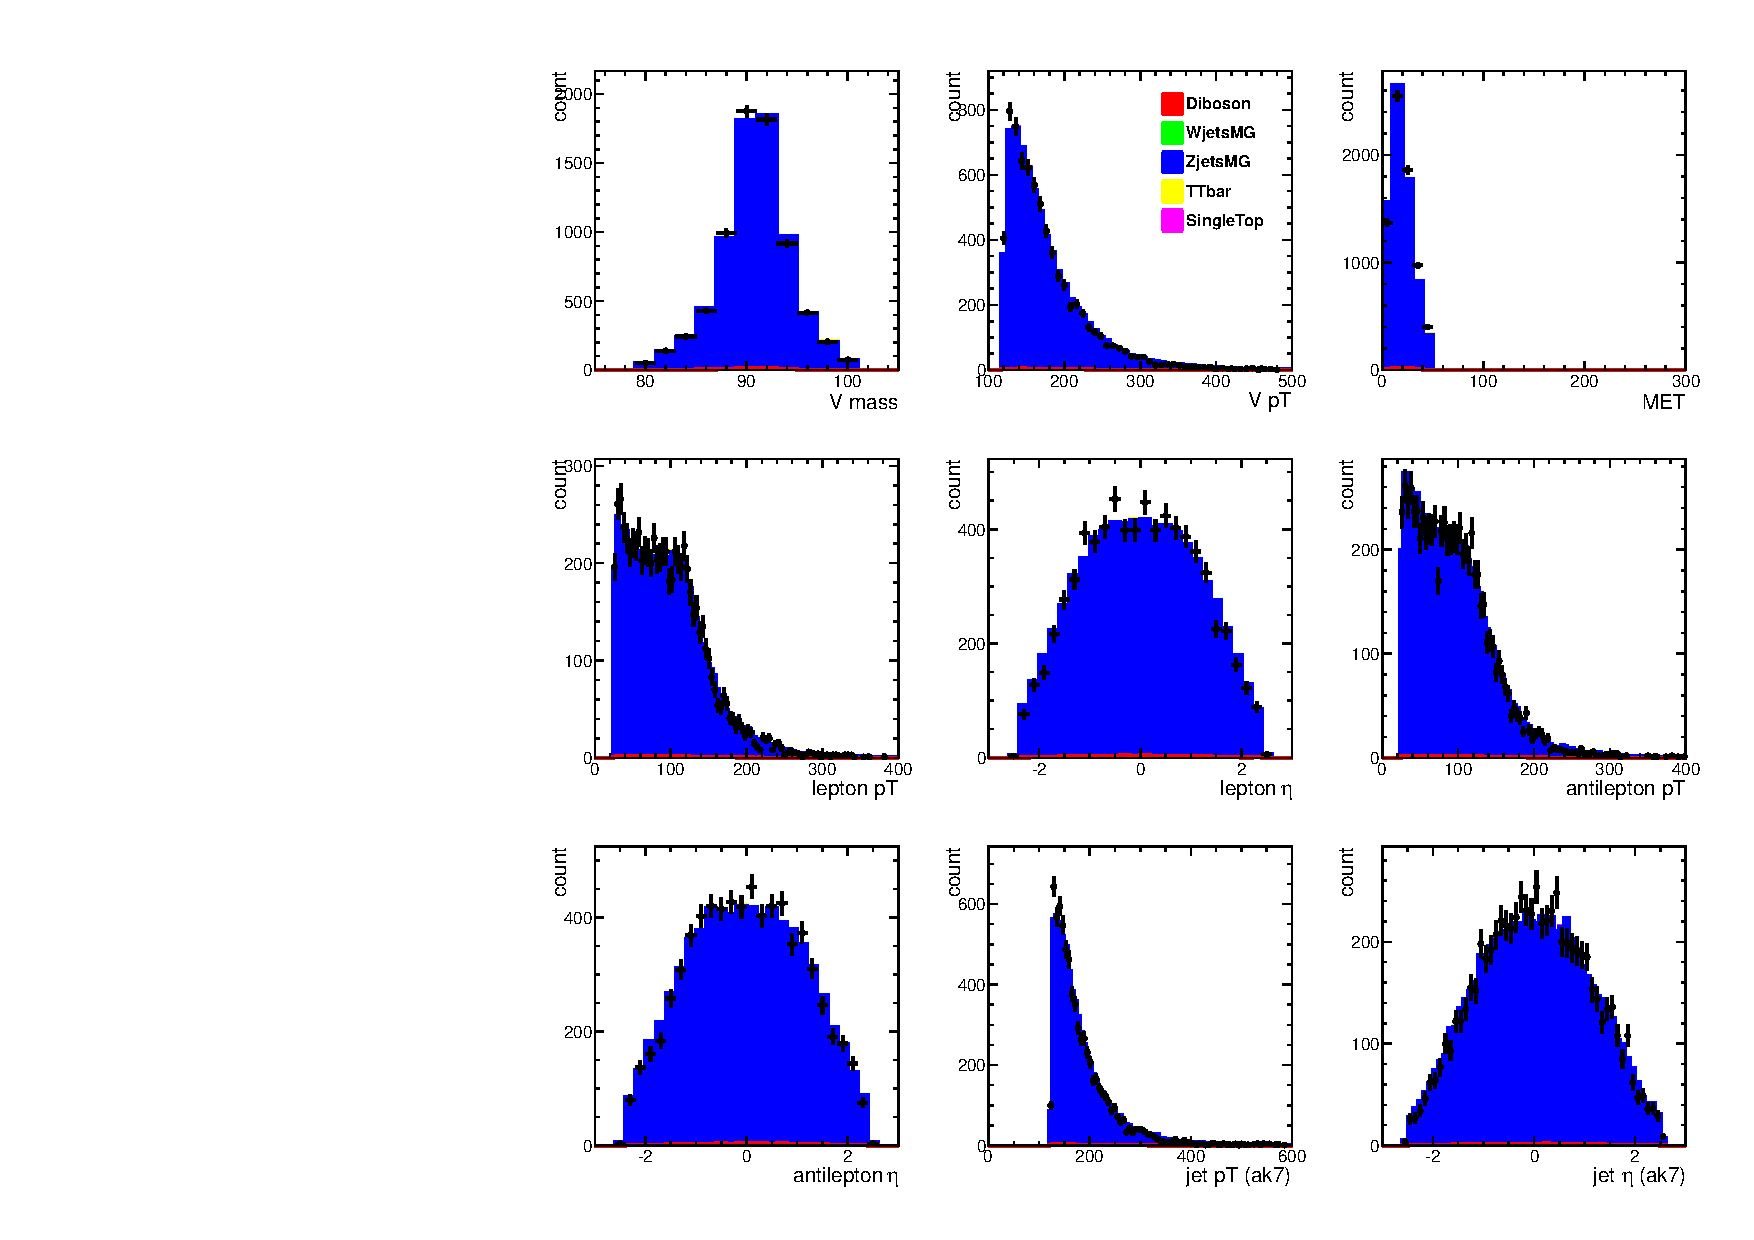
\includegraphics[width=1.0\textwidth]{figs/kinematics_stack_ak7_Zmumu.pdf}
\caption{Kinematic distributions for $Z(\mu\mu)$+ jet events. In clockwise order from top left: di-lepton invariant mass, vector boson $p_T$, MET, $p_T (\mu^-)$ and $\eta (\mu^-)$, $p_T (\mu^+)$ and $\eta (\mu^+)$, AK7 jet $p_T$ and $\eta$.}
\label{figs:kin1}
\end{figure}

\begin{figure}[htb]
\centering
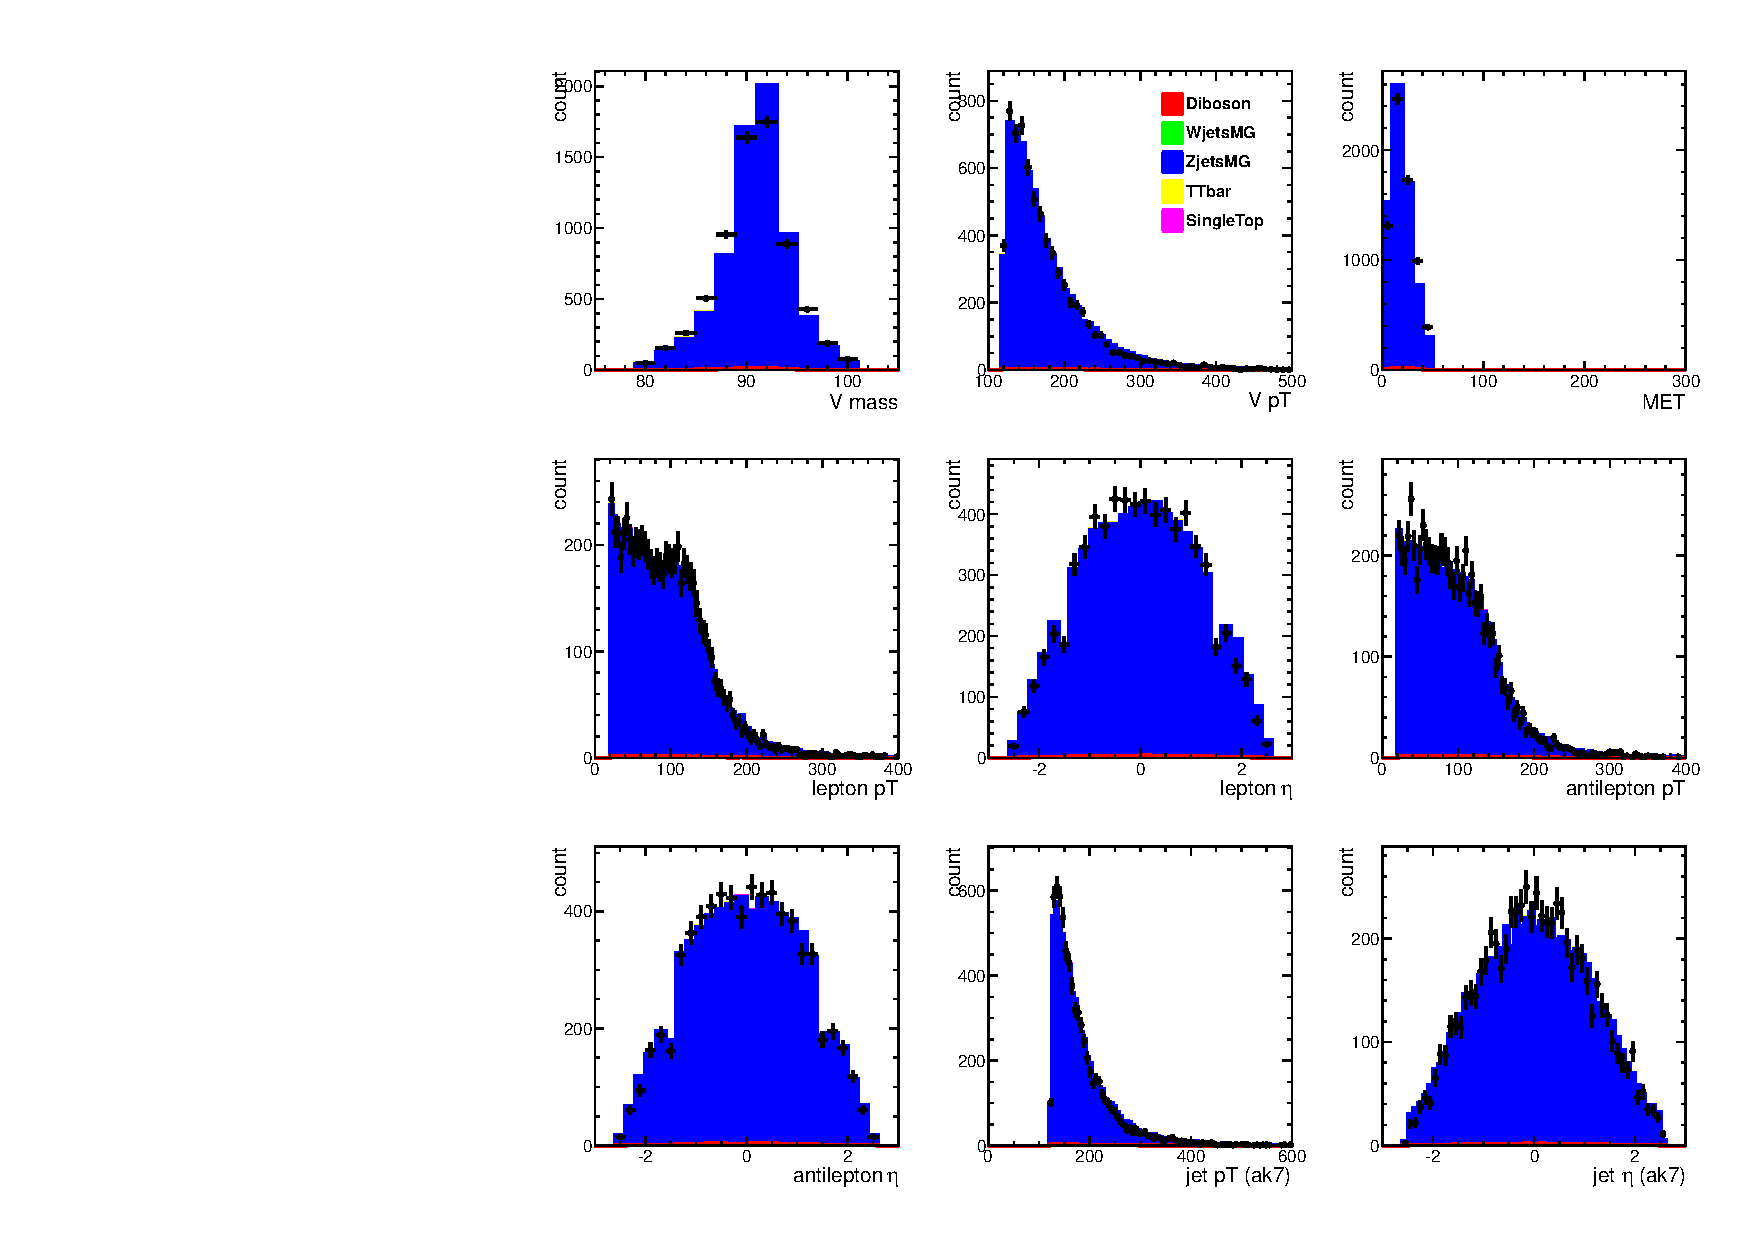
\includegraphics[width=1.0\textwidth]{figs/kinematics_stack_ak7_Zee.pdf}
\caption{Kinematic distributions for $Z(ee)$+ jet events. In clockwise order from top left: di-lepton invariant mass, vector boson $p_T$, MET, $p_T (e^-)$ and $\eta (e^-)$, $p_T (e^+)$ and $\eta (e^+)$, AK7 jet $p_T$ and $\eta$.}
\label{figs:kin2}
\end{figure}

\begin{figure}[htb]
\centering
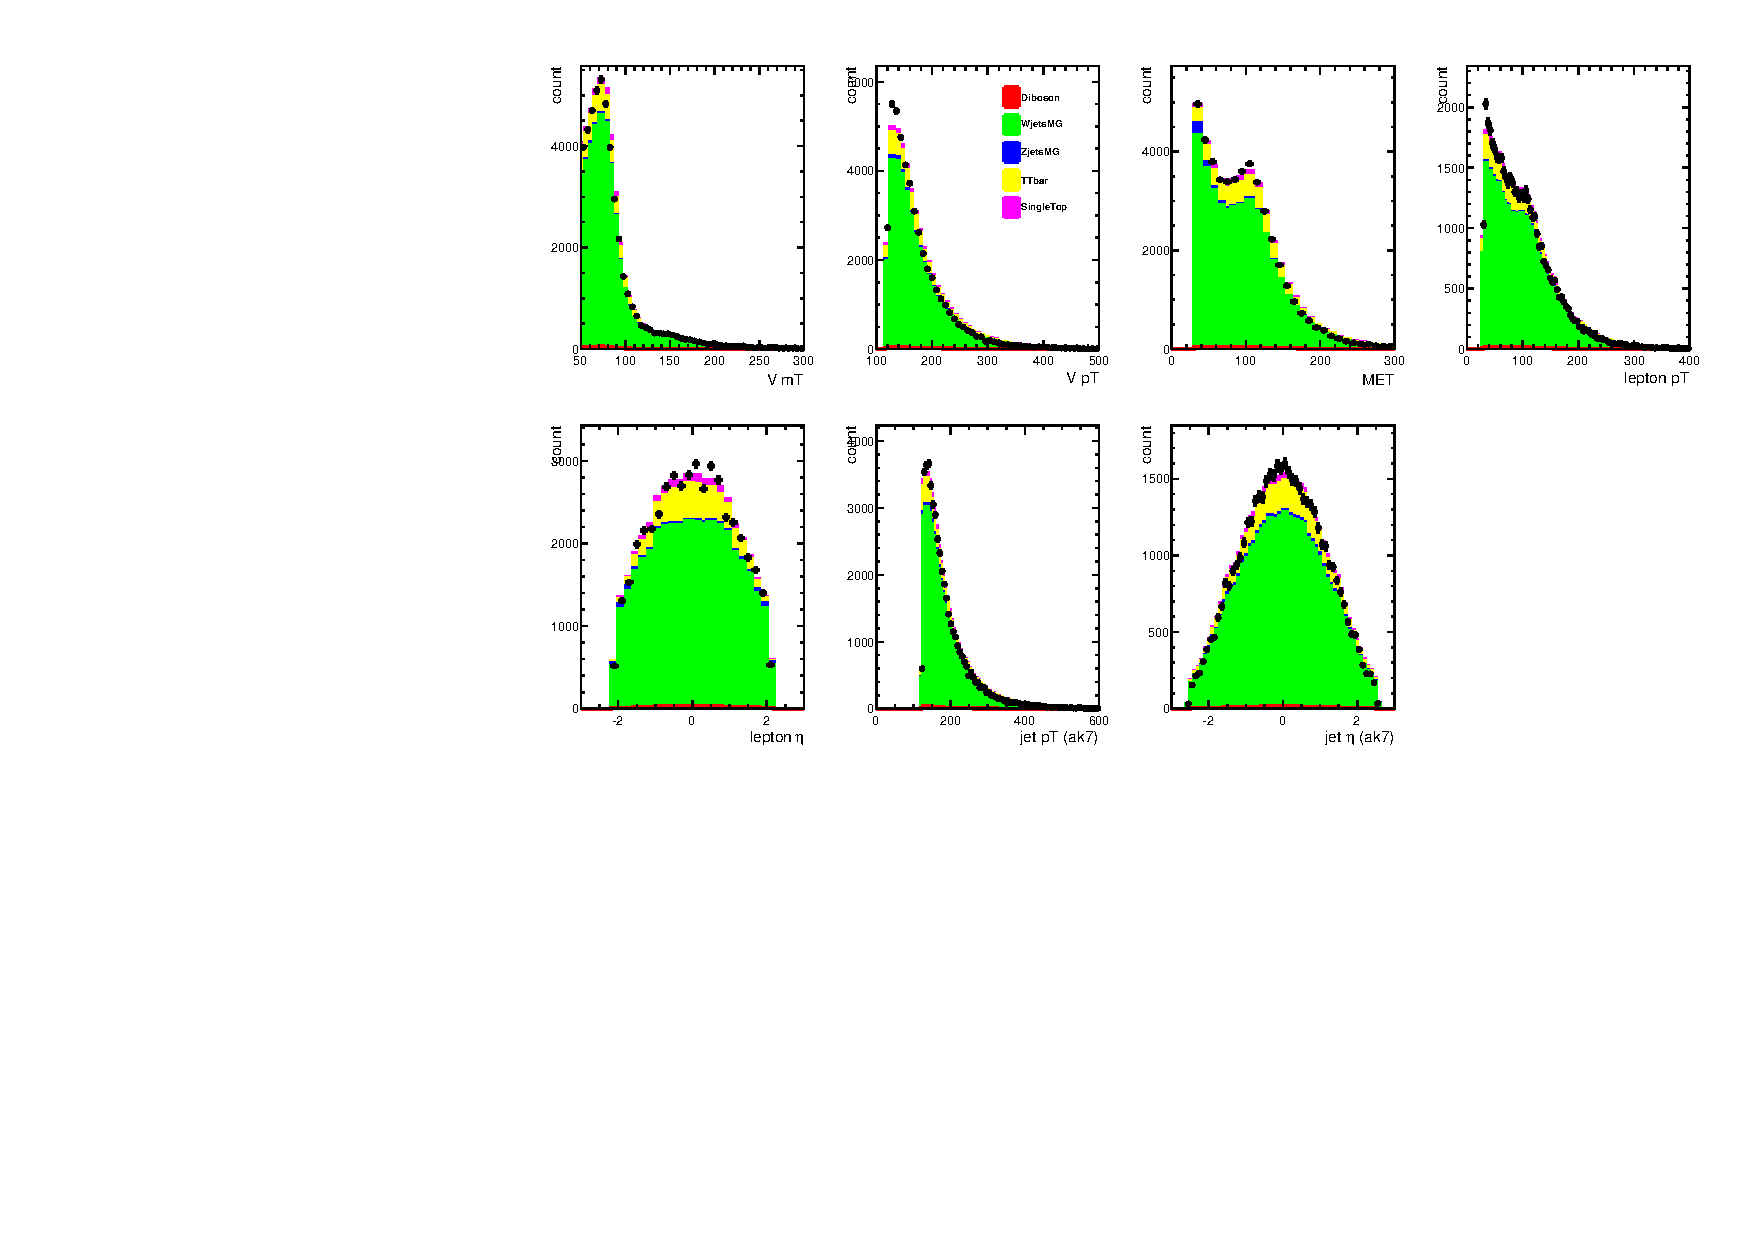
\includegraphics[width=1.0\textwidth]{figs/kinematics_stack_ak7_Wmunu.pdf}
\caption{Kinematic distributions for $W(\mu\nu)$+ jet events. In clockwise order from top left: $W$ transverse mass, vector boson $p_T$, MET, $p_T (\mu^-)$ and $\eta (\mu^-)$, AK7 jet $p_T$ and $\eta$.}
\label{figs:kin3}
\end{figure}

\begin{figure}[htb]
\centering
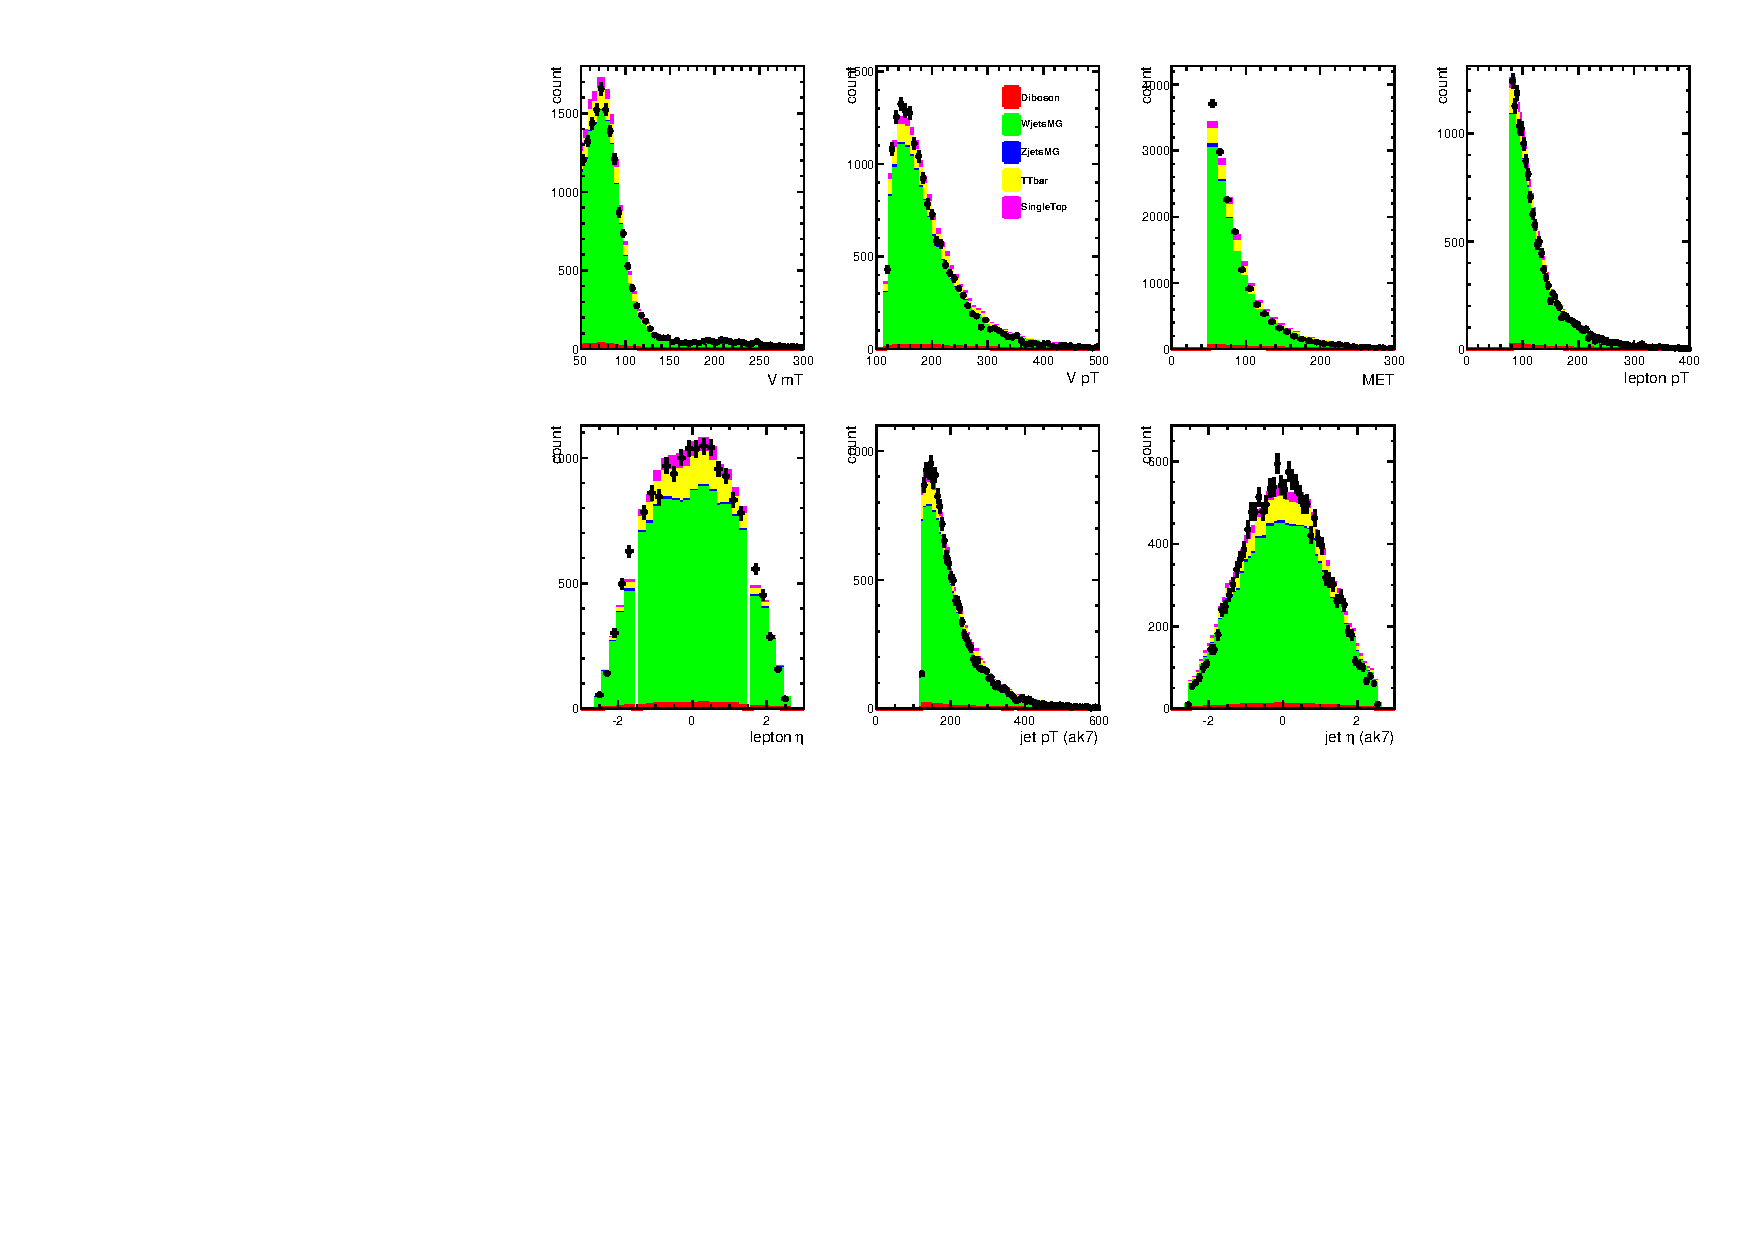
\includegraphics[width=1.0\textwidth]{figs/kinematics_stack_ak7_Wenu.pdf}
\caption{Kinematic distributions for $W(e\nu)$+ jet events. In clockwise order from top left: $W$ transverse mass, vector boson $p_T$, MET, $p_T (e^-)$ and $\eta (e^-)$, AK7 jet $p_T$ and $\eta$.}
\label{figs:kin4}
\end{figure}


Corresponding kinematic distributions requiring different leading jet types are shown in Appendix~\ref{app:kinematic}. 



%\section{Validation using anti-kT 5 Jets}

\section{Jet algorithm comparisons}
\subsection{Sequential jet-clustering algorithms}
\label{sec:algos}

In this analysis, jets are clustered with sequential jet-clustering algorithms. 
In these algorithms, the four-vectors of input particles are combined pairwise, 
via four-vector addition, until a final jet
is found. Specifically, for each pair of input particles $i$ and $j$,
two quantities are computed, the first is a distance measure between
the two particles, and the second is the so-called ``beam distance''
of each particle:

\begin{eqnarray}
\label{eq:dij}
d_{ij} &=& \mathrm{min}({\pt}_i^{2n},{\pt}_j^{2n}) \Delta R_{ij}^2 / R^2 \\
d_{iB} &=& {\pt}_i^{2n}
\end{eqnarray}

where $\pt$ is the transverse momentum, 
$\Delta R = \sqrt{(\Delta \eta_{ij})^2 + (\Delta\phi_{ij})^2 }$
is the angular distance between the two particles $i$ and $j$,
and $R$ is an order-unity parameter chosen for the algorithm.

The value for $n$ is a parameter of the algorithm in question and
governs the shape of the jets.
The first such sequential combination algorithm is called the
$k_{\mathrm{T}}$ (KT) algorithm and has $n=1$. These jets are typically irregularly
shaped and are useful for reconstructing lower momentum jets~\cite{ktalg}. 
The second such algorithm
is called the anti-$k_{\mathrm{T}}$ (AK) algorithm and has $n=-1$. This algorithm
behaves like an idealized cone algorithm, and are used extensively
at the LHC experiments and elsewhere~\cite{ktalg}. The third such
algorithm is called the Cambridge-Aachen (CA) algorithm and has $n=0$. This
algorithm uses only angular information, and like the $k_\mathrm{T}$ algorithm
has irregularly-shaped jets. The CA algorithm is very useful for distinguishing
jet substructure~\cite{CAcambridge,CAaachen}.

Jet grooming - elimination of uncorrelated UE/PU radiation from a target jet - is useful irrespective of the specific 
boosted particle search and can even be applied for slow-moving heavy particles that decay to well-separated jets. 
We consider in this analysis three different forms of grooming: trimming, pruning and filtering. 

There are choices of what jet algorithm (KT, AK, or CA) can be used by all of these grooming
algorithms. These algorithms can use different jet algorithms for jet finding and the
substructure determination. We have chosen to cluster our jets with the anti-$k_{\mathrm{T}}$
algorithm with $R=0.7$ (AK7), as these are extensively studied at CMS. 
Comparisons of AK jets with $R=0.5$ (AK5) AND $R=0.8$ (AK8)
are also investigated, 
as well as
with the CA algorithm with $R$=0.8 (CA8) and $R$=1.2 (CA12). The latter
two are compared because of their usage in other CMS analyses~\cite{EXO-11-006,HIG-11-XX}. 
After the initial jet clustering, the choice of algorithm
for the substructure determination depends on the algorithm chosen and is described
in detail below. 

\subsection{Pruning algorithm}

Pruning was introduced by Ellis, Vermilion and Walsh~\cite{pruning}-\cite{pruning2}. 
In our implementation, after
the jets are clustered with the AK7 algorithm, the pruning algorithm reclusters the constituents
of the AK7 jet with the CA algorithm, with extra
veto conditions applied in addition to the standard conditions in Equation~\ref{eq:dij}. 
The particle is vetoed if either of the following two conditions are met:

\begin{eqnarray}
z_{ij} & = & \frac{\mathrm{min}({\pt}_i,{\pt}_j)}{{\pt}_{i+j}} < z_{\mathrm{cut}} \\
\Delta R_{ij} & < & D_{\mathrm{cut}} = \alpha \times \frac{m_J}{{\pt}_J}
\end{eqnarray}

where ${\pt}_i$ and ${\pt}_j$ are the transverse momentum of the constituents,
${\pt}_{i+j}$ is the transverse momentum of the four-vector sum of those constituents,
$m_J$ and ${\pt}_J$ are the mass and transverse momentum of the AK7 jet, 
and $z_{\mathrm{cut}}$ and $\alpha$ are parameters of the algorithm, 
chosen to be 0.1 and 0.5, respectively. 

\subsection{Trimming algorithm}

Trimming is a technique that ignores particles within a jet that fall below 
a dynamic $\pt$ threshold. It was introduced by Krohn, Thaler and Wang in~\cite{trimming}. 
Trimming reclusters the jets's constituents with the $k_{\mathrm{T}}$ 
algorithm with a radius 
$R_{sub}$ and then accepts only the subjets that have 
${\pt}_{sub} > f_{cut}$, where $f_{cut}$ is taken proportional 
either to the jet's $\pt$ or to the event's total$H_T$.
The values $R_{sub}$ and $f_{cut}$ are parameters of the algorithm,
taken to be 0.2 and 0.03, respectively. 



\subsection{Filtering algorithm}

The filtering procedure aims to identify relatively hard, symmetric splittings in a jet that contribute significantly to the jet invariant mass. This procedure is taken from recent Higgs search studies~\cite{boostedHiggs}. The parameters are tuned to maximise sensitivity to a Standard Model Higgs boson decaying to $b\bar{b}$, but this procedure is suitable generally for identifying two-body decay processes. The effect of the procedure is to search for jets where the clustering process combined two relatively low mass objects to make a much more massive object. This indicates the presence of a heavy particle decay. The procedure then attempts to retain only the constituents believed to be related to the decay of this particle.
The identification strategy proposed in~\cite{boostedHiggs} uses the inclusive, longitudinally invariant CA algorithm to flexibly adapt to the fact that the two-jet angular separation varies significantly with 
the heavy particle $\pt$ and decay orientation. In this algorithm the angular distance 
$\Delta R^2_{ij} = (\Delta \eta_{ij} )^2 + (\Delta \phi_{ij} )^2$, 
where $y$ is the pseudorapidity and $\phi$ the azimuthal angle, is calculated between all 
pairs of objects $i$ and $j$. The closest pair is combined into a single object, the set of distances is 
updated, and the procedure is repeated until all objects are separated by a $\Delta R_{ij} > R$, where $R$ 
is a parameter of the algorithm. This provides a hierarchical structure for the clustering, like the 
$k_{\mathrm{T}}$ algorithm but in angles rather than in relative transverse momenta.
%Each stage in the clustering combines two objects $i$ and $j$ to make another object $j$. 
We use the definition $v = \frac{min({\pt}_i^2,{\pt}_j^2) }{m^2_{i+j}} \Delta R^2$. The procedure takes a
jet to be the object $j$ and applies the following:
\begin{enumerate}
\item Undo the last clustering step of $i+j$ to get $i$ and $j$. These are ordered such that their mass has the property $m_{i} > m_{j}$. If $i+j$ cannot be unclustered (i.e. it is a single particle) then it is not a suitable candidate, so discard this jet.
\item  If the splitting has $m_{i}/m_{i+j} < \mu$ (large change in jet mass) and $v > v_{cut}$ (fairly symmetric) then continue, otherwise redefine $i+j$ as $i$ and go back to step 1. Both $\mu$ and $v_{cut}$ are parameters of the algorithm.
\item  Recluster the constituents of the jet with the CA algorithm with an $R$-parameter of $R_{filt} =\mbox{min} (0.3, \Delta R^2_{ij} /2)$ finding $n$ new subjets $s_1, s_2 ...s_n$ ordered in descending $\pt$.
\item  Redefine the jet as the sum of subjet four-momenta $\sum_{i=1}^{min(n,3)} s_i$
\end{enumerate}

\noindent The algorithm parameters $\mu$ and $v_{cut}$ are taken as 0.67 and 0.09 respectively.
The $\mu$ cut attempts to identify a hard structure in the distribution of energy in the jet, which would imply the decay of a heavy particle. The cut on $v$ further helps by suppressing very asymmetric decays of the type favoured by splittings of quarks and gluons.
Steps 3 and 4 filter out some of the particles in the candidate jet, the aim being to retain particles relevant to the hard process while reducing the contribution from effects like underlying event and pile-up. The 4-vector after step 4 can be treated like a new jet. This new jet has a $\pt$ and mass less than or equal to those of the original jet.


\subsection{AK jet mass distributions}

The results on the jet mass distributions in this section and below are reported in several different $p_T$ regions for the leading jet: $(1) 125 < p_T < 200$ GeV, $(1) 200 < p_T < 300$ GeV, $(1) 300 < p_T < 400$ GeV, and $(1) p_T >400$ GeV.
We start by showing in fig.~\ref{figs:allAlgos1}-\ref{figs:allAlgos3} the reconstructed ``raw'' ungroomed and grommed mass distributions on data for AK5, AK7 and AK8 jets.

\begin{figure}[!htb]
\centering
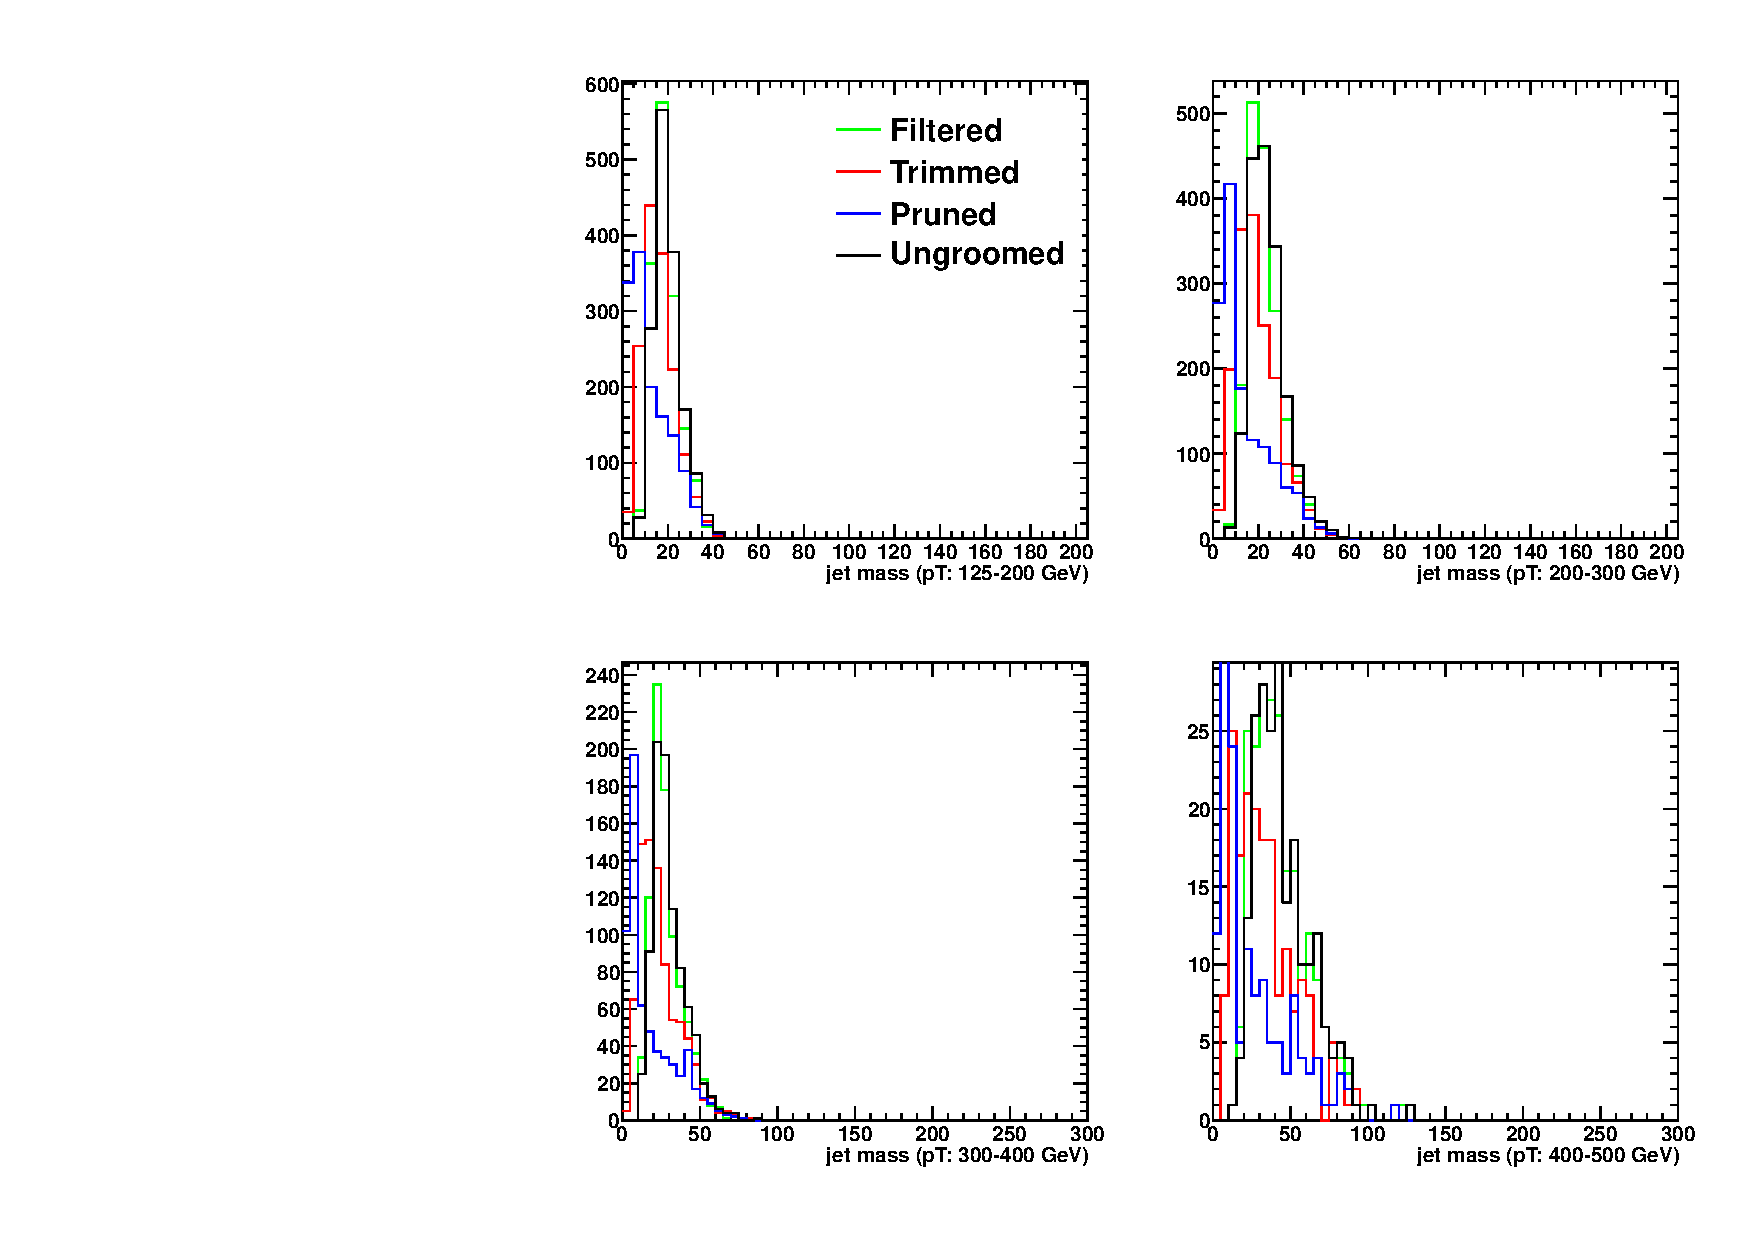
\includegraphics[width=1.0\textwidth]{figs/allAlgos_2x2PtBins_ak5.pdf}
\caption{Raw jet mass distribution on data for the leading AK5 (ungroomed or groomed) jet in different jet momentum regions.}
\label{figs:allAlgos1}
\end{figure}

\begin{figure}[!htb]
\centering
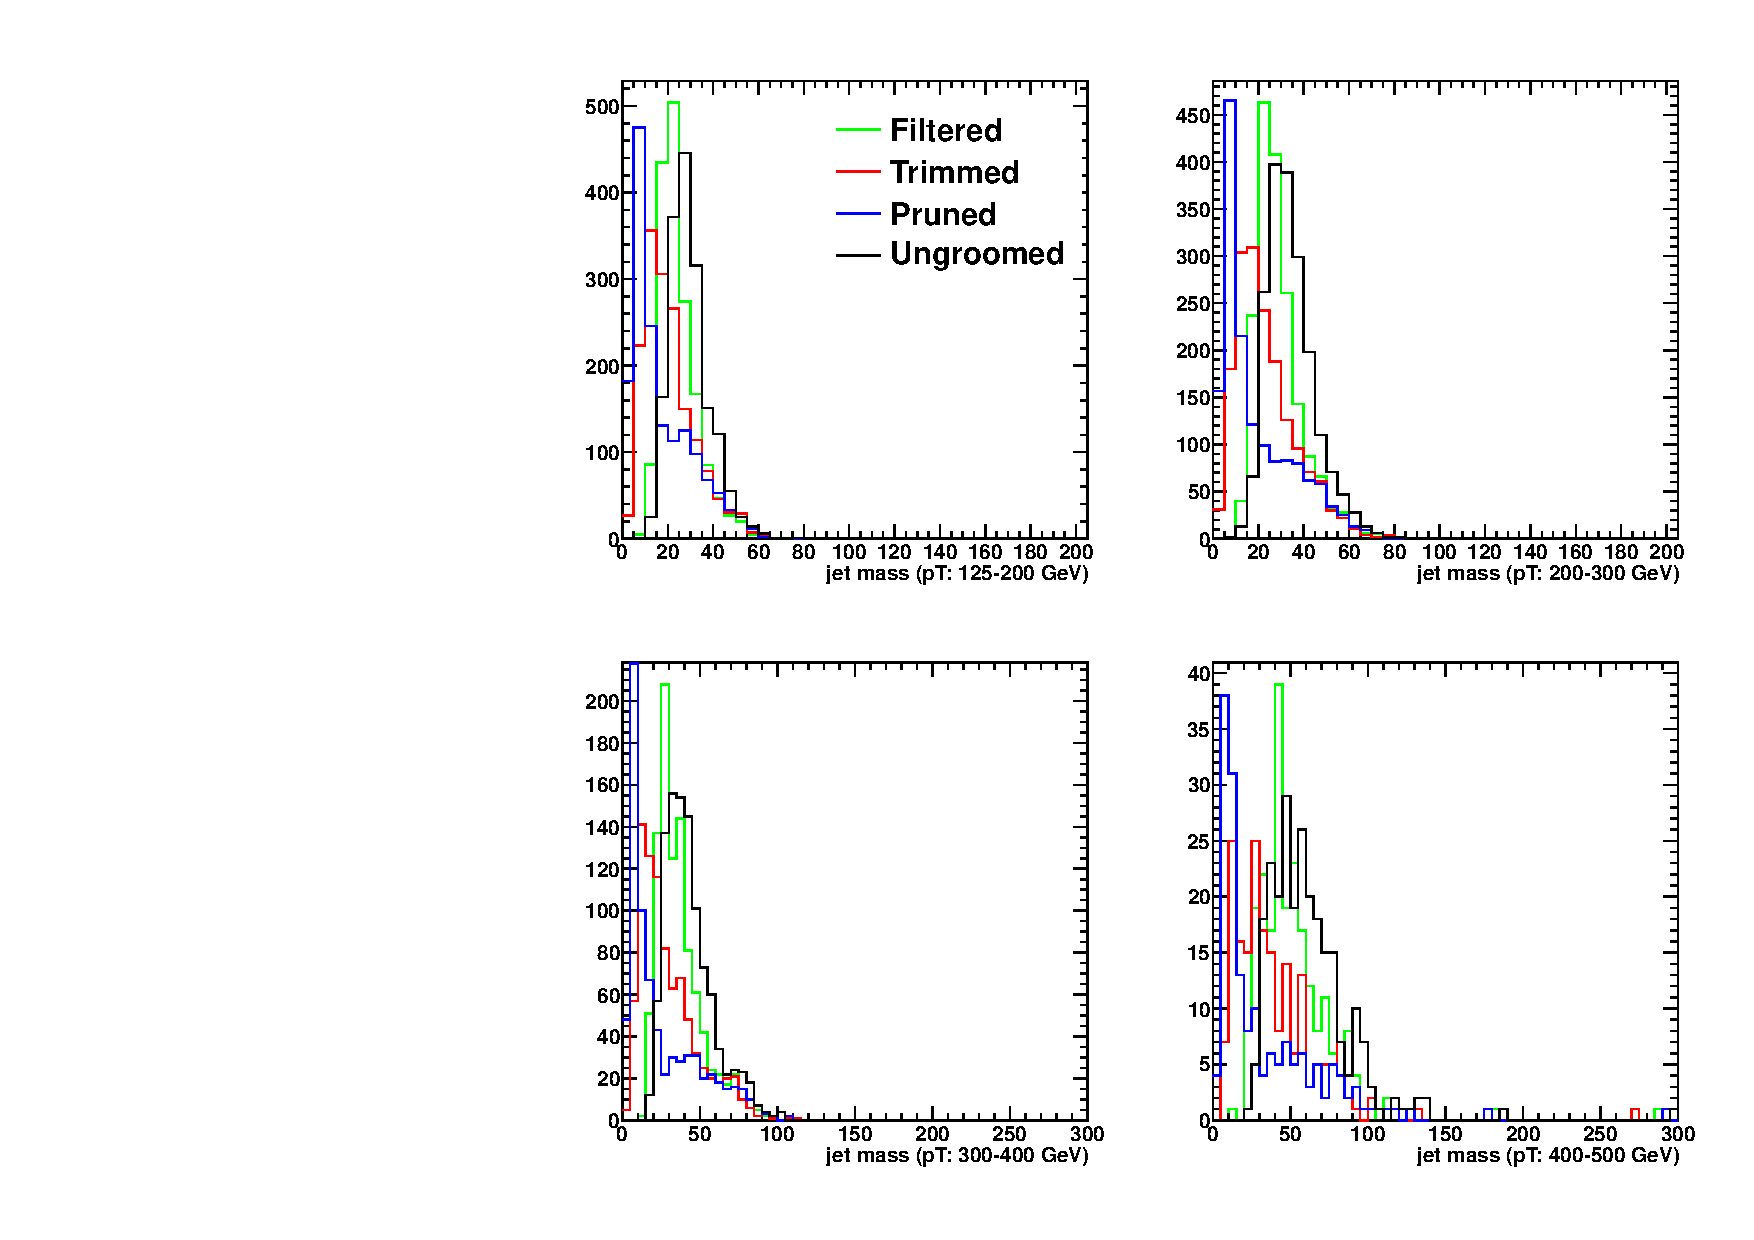
\includegraphics[width=1.0\textwidth]{figs/allAlgos_2x2PtBins_ak7.pdf}
\caption{Raw jet mass distribution on data for the leading AK7 (ungroomed or groomed) jet in different jet momentum regions.}
\label{figs:allAlgos2}
\end{figure}

\begin{figure}[!htb]
\centering
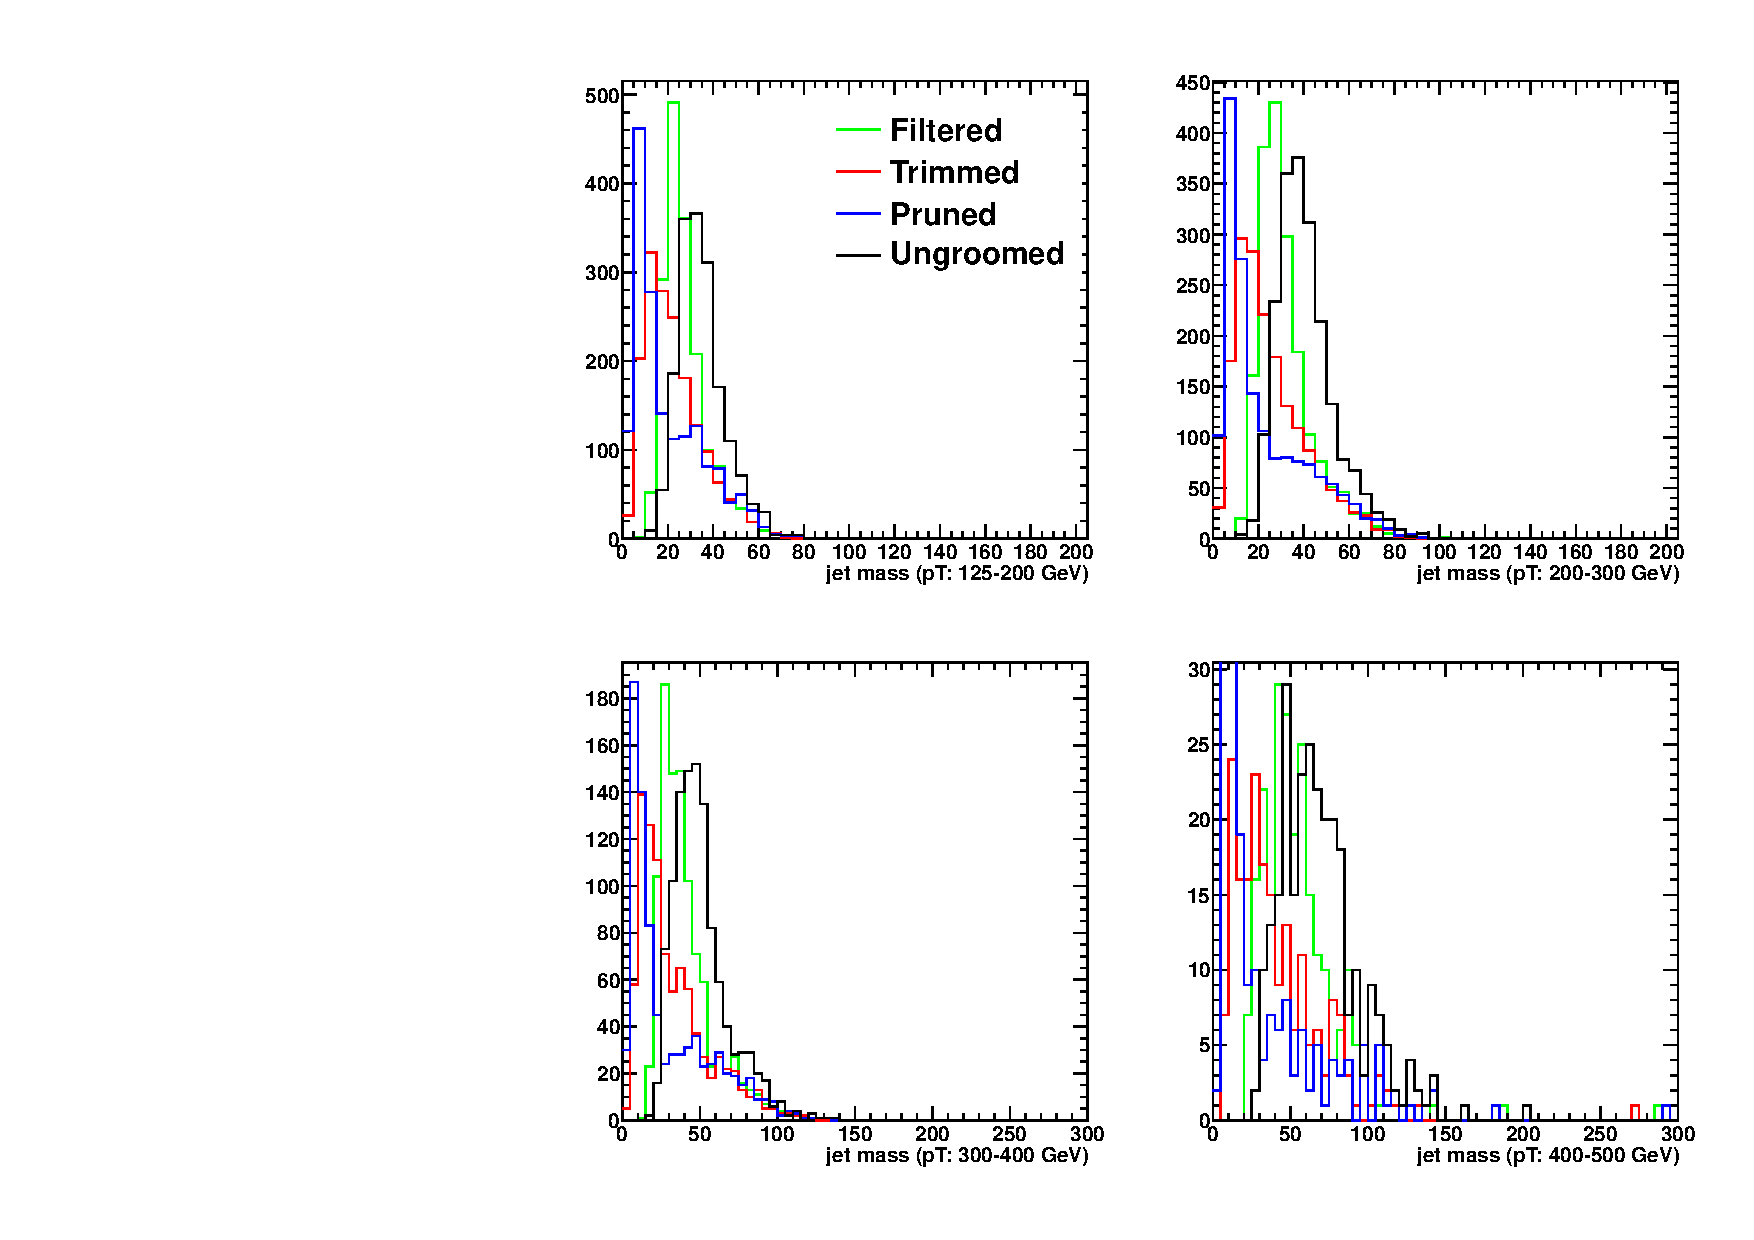
\includegraphics[width=1.0\textwidth]{figs/allAlgos_2x2PtBins_ak8.pdf}
\caption{Raw jet mass distribution on data for the leading AK8 (ungroomed or groomed) jet in different jet momentum regions.}
\label{figs:allAlgos3}
\end{figure}



 

\ifnpas
\section{Algorithmic Characterization}
\fi
\label{sec:algo_char}

In order to use the substructure tools that have been presented above, 
it is necessary to measure several supporting numbers.
The first is the subjet energy scale. 
%The second is the selection efficiency of the substructure tools in the
%data (compared to the Monte Carlo). The third is the rate at which generic 
%QCD jets fake the selection (the ``mistag rate''). 

\ifnpas
\subsection{Subjet energy scale}
\fi 
\label{sec:substructure_jec}




\ifnpas

The prescription we have followed to correct our jets is to apply the
\verb!AK5PFchs! corrections to our jets. This is not exactly correct
because we are using jets built with different clustering algorithms and different cone size (0.7, 0.8, 1.2).
However, these are the only corrections that are sufficiently commissioned
for usage. There is not expected to be a large difference in response between
these types of jets in a boosted kinematical regime.

Figure~\ref{figs:ptRatio} 
shows the comparison of the reconstructed jet momentum (corrected to {\tt L1FastJet, L2Relative, L3Absolute}) scale and 
resolution by comparing to the generator level jets for AK5, AK7 and AK8 generator level jets, where the  generator
level jets have no substructure
algorithms applied. This means that in each plot the ungroomed distributions show the scale and resolution for AK5, AK7 and AK8 jet compared to the matching same radius generator jets, while for the groomed jets we use the same ungroomed ``denominator''.  
The scale and resolution are obtained by ``slicing'' the jet $p_T$ or pseudorapidity distributions and performing gaussian fits of the reconstructed/generated ratio distributions. We then report the mean (scale offset) and sigma (resolution) from these fits as a function of the jet $p_T$ or pseudorapidity.
  
We can notice that the response for filtered jet is the closest to the ungroomed jets response (always within less than 5\%). 
The response becomes reasonably flat in the boosted regime above 200-250 GeV, apart for the pruned jets (and in a less evident way for the trimmed). 
The jet pruning and trimming (intentionally) removes part
of the jet, and that fraction is larger at lower momenta. If one compares the
response of jet-pruned reconstructed jets with respect to unpruned
generator-level jets, a large difference is seen at low $\pt$ (maximally 8\%).
 
\begin{figure}[!htb]
\centering
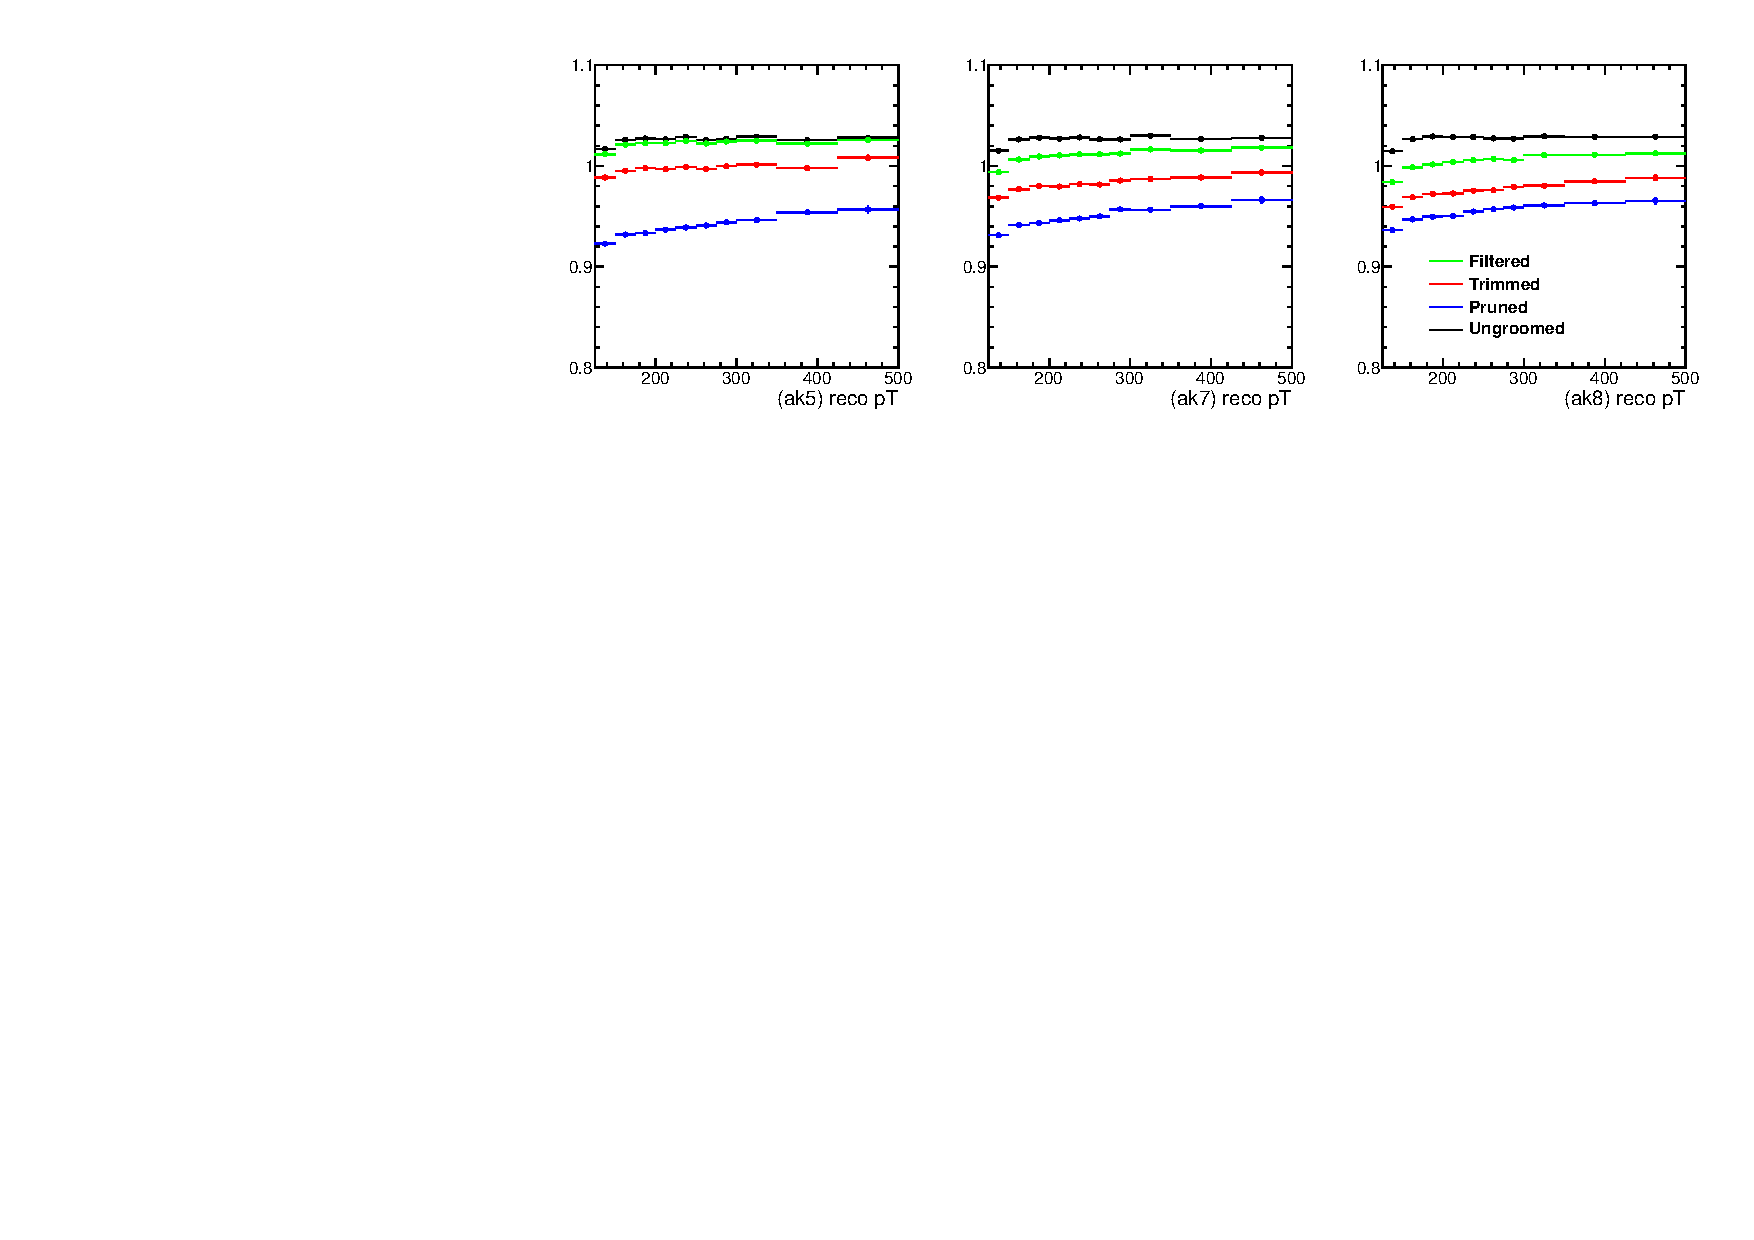
\includegraphics[width=1.0\textwidth]{figs/ptRatioVsPt_mean.pdf}
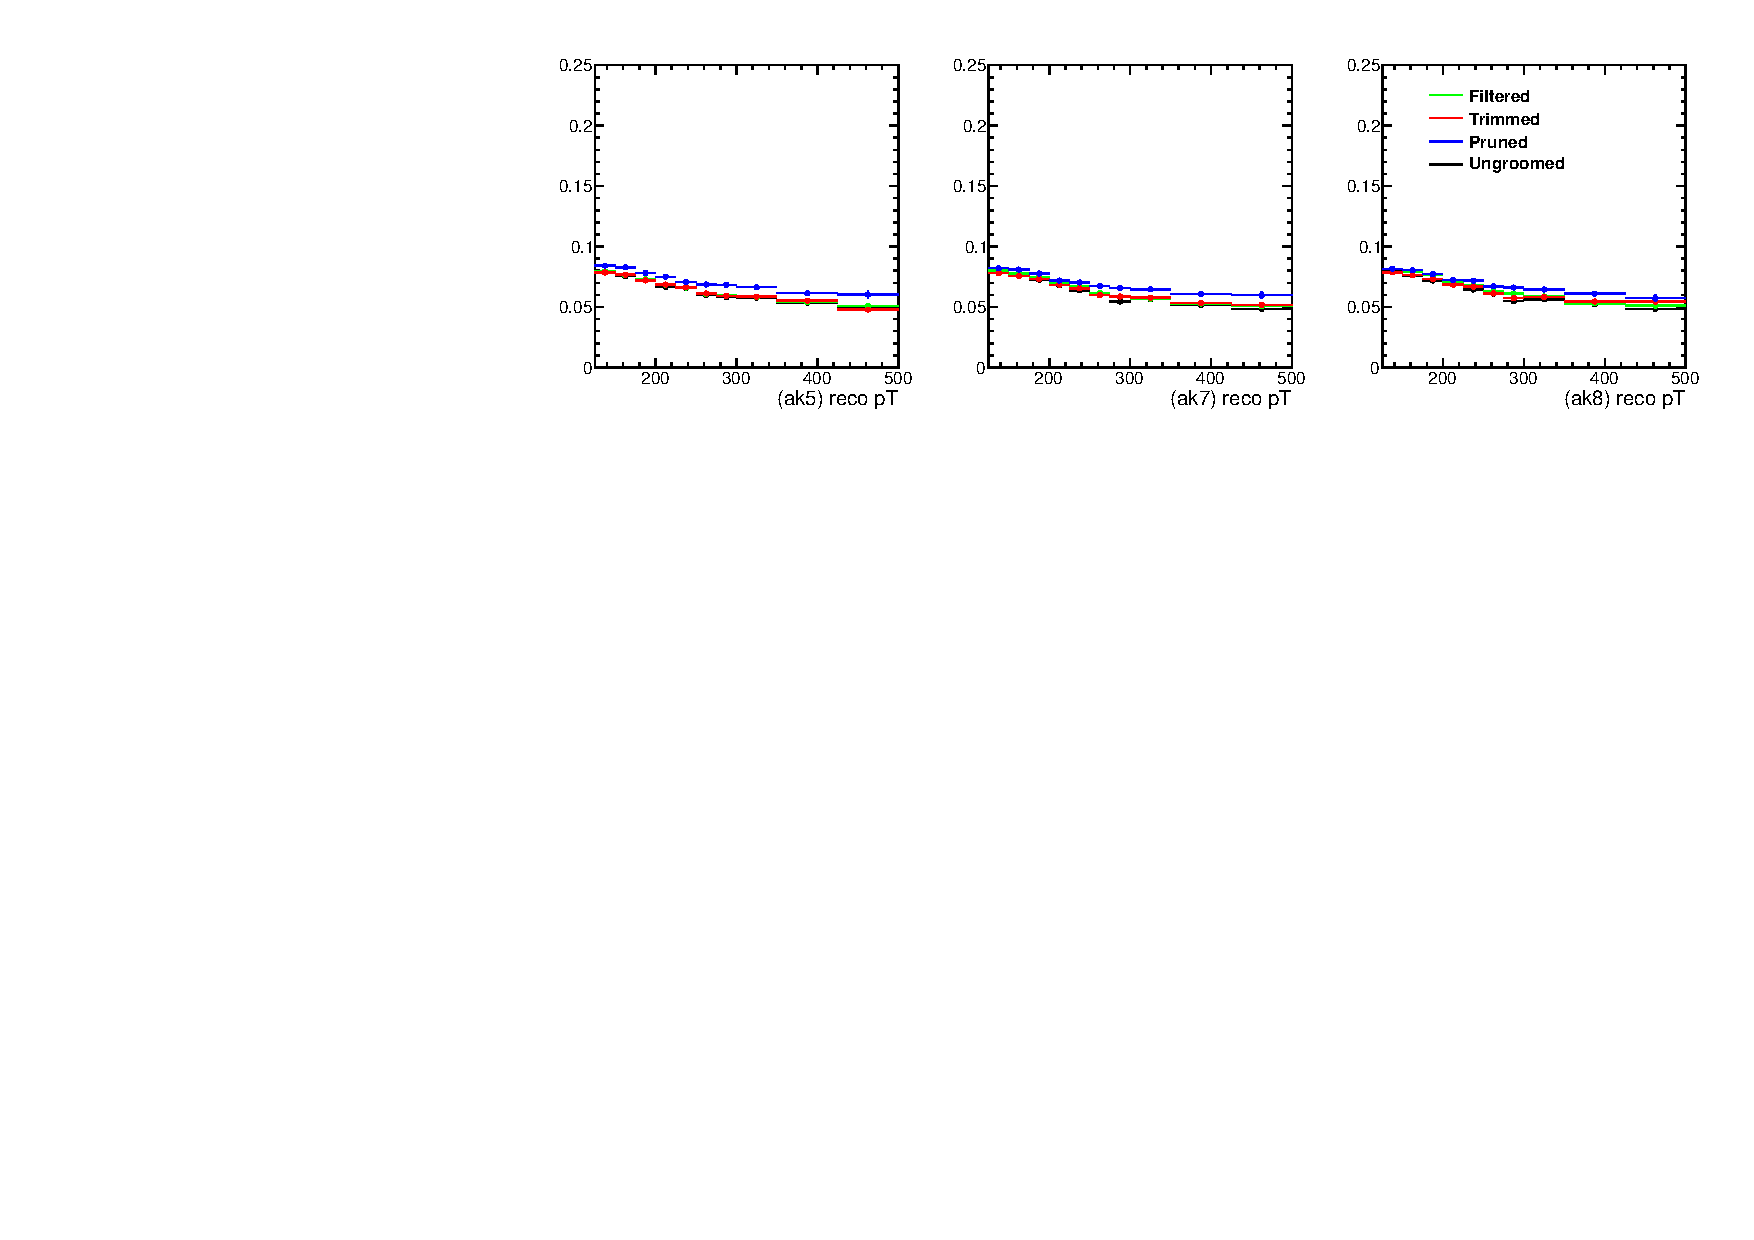
\includegraphics[width=1.0\textwidth]{figs/ptRatioVsPt_sigma.pdf}
\caption{Jet response (top: scale offset, bottom: resolution) for different jet algorithms as a function of the jet momentum. Here, the
  substructure algorithms are compared to the
  generator-level AK5, AK7 and AK8 jets without the substructure algorithms applied.}
\label{figs:ptRatio}
\end{figure}


Figure~\ref{figs:ptRatiovsEta} shows the corresponding distributions as a function of the ungroomed generated jet pseudorapidity. The noticeable behaviour in the groomed jets is a residual dependence in the resolution in the forward region, that becomes more and more pronounced the more aggressive the grooming is. Most likely, the effect, around 2\%, is due to a residual clustering dependence that is not present in the ungroomed jet corrections.  
Figure~\ref{figs:ptRatiovsPV} shows the jet momentum resolution as a function of the primary vertex multiplicity, and it shows the same PU dependency for groomned and ungroomed jets.  
 

%\includegraphics[width=1.0\textwidth]{figs/ak5ca8compare_genunpruned_jetResAvg}
%\caption{Jet response for different jet algorithms. Here, the
%  substructure algorithms are compared to the unmodified
%  generator-level jets ({\tt AK5GenJets} and {\tt CA8GenJets} for
%  the AK5 and CA8 algorithms, respectively).}
%\label{figs:ak5ca8compare_genunpruned_jetResAvg}
%\end{figure}


\begin{figure}[htb]
\centering
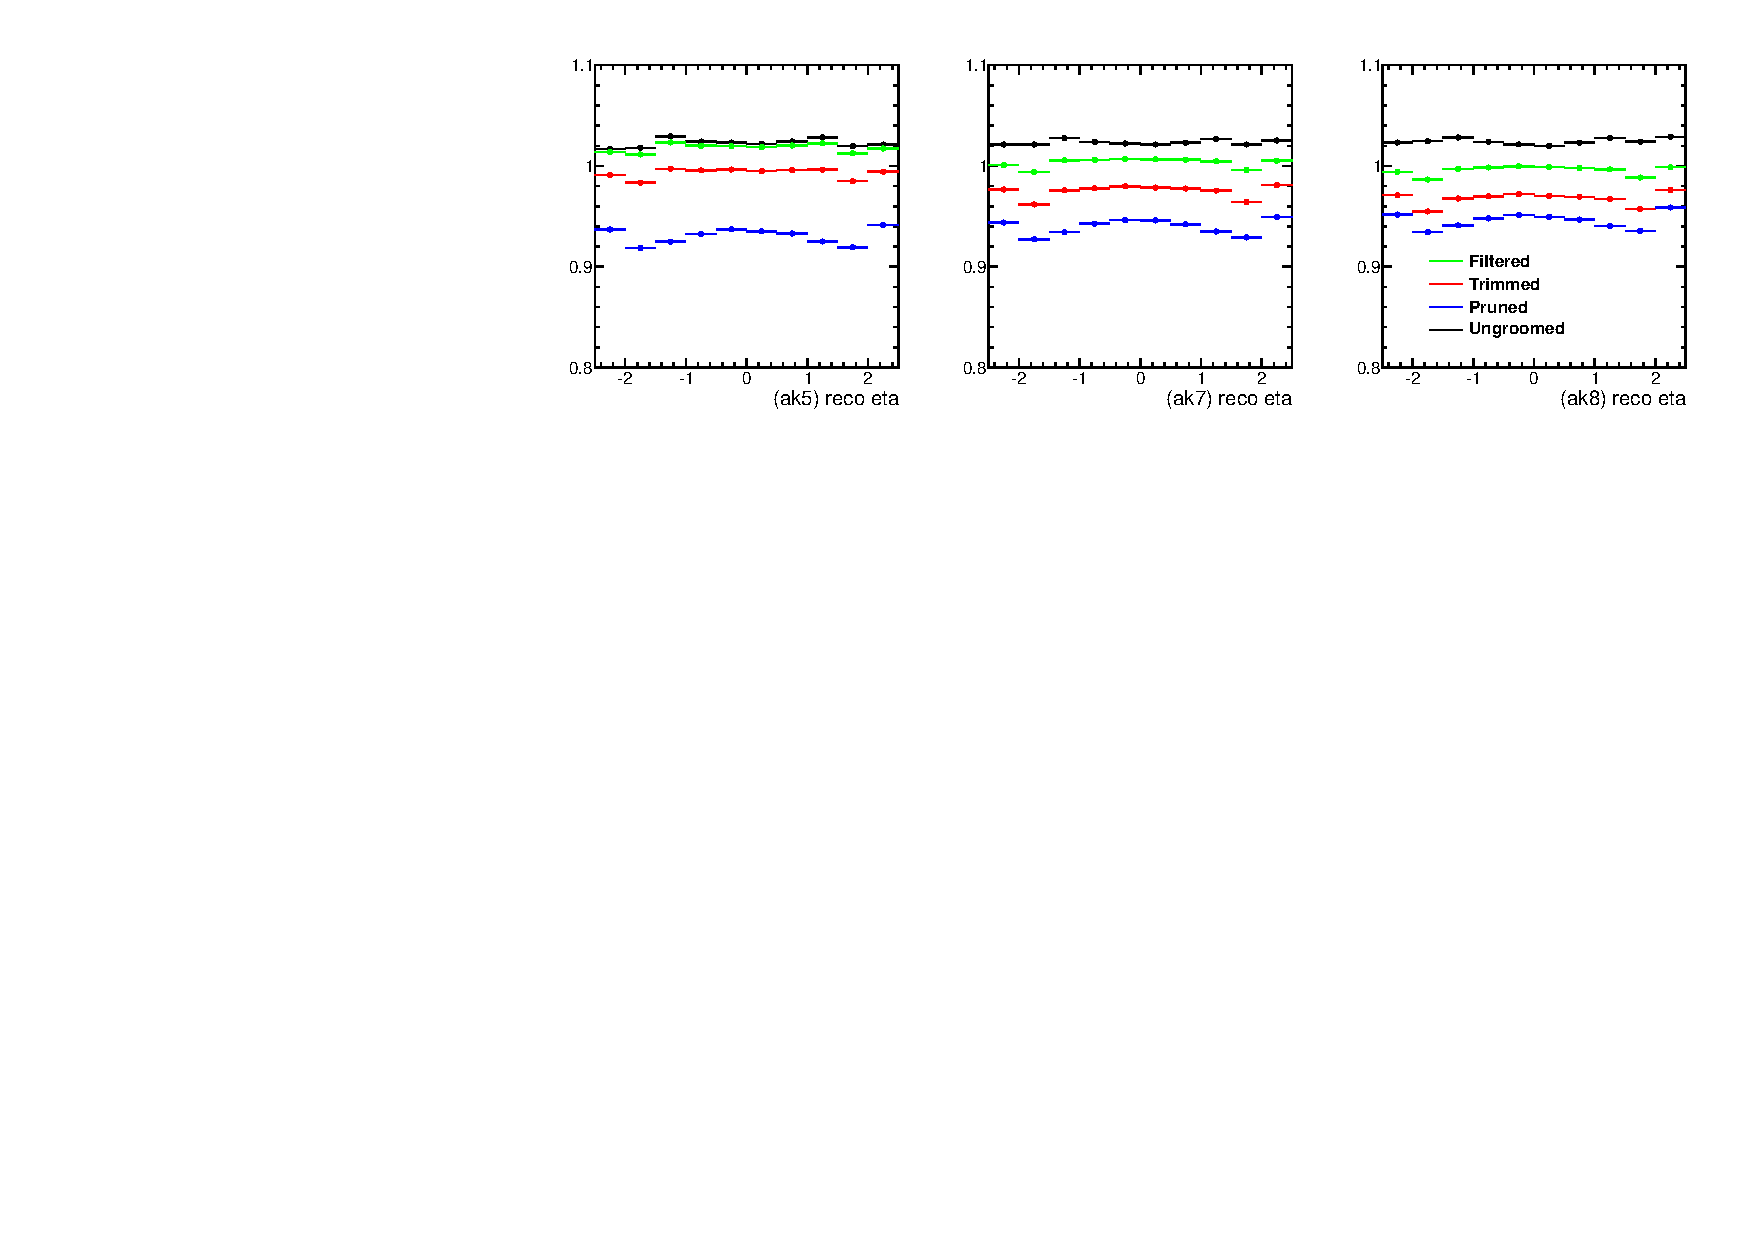
\includegraphics[width=1.0\textwidth]{figs/ptRatioVsEta_mean.pdf}
\caption{Jet response for different jet algorithms as a function of the jet pseudorapidity. Here, the
  substructure algorithms are compared to the
  generator-level AK5, AK7 and AK8 jets without the substructure algorithms applied.}
\label{figs:ptRatiovsEta}
\end{figure}

\begin{figure}[htb]
\centering
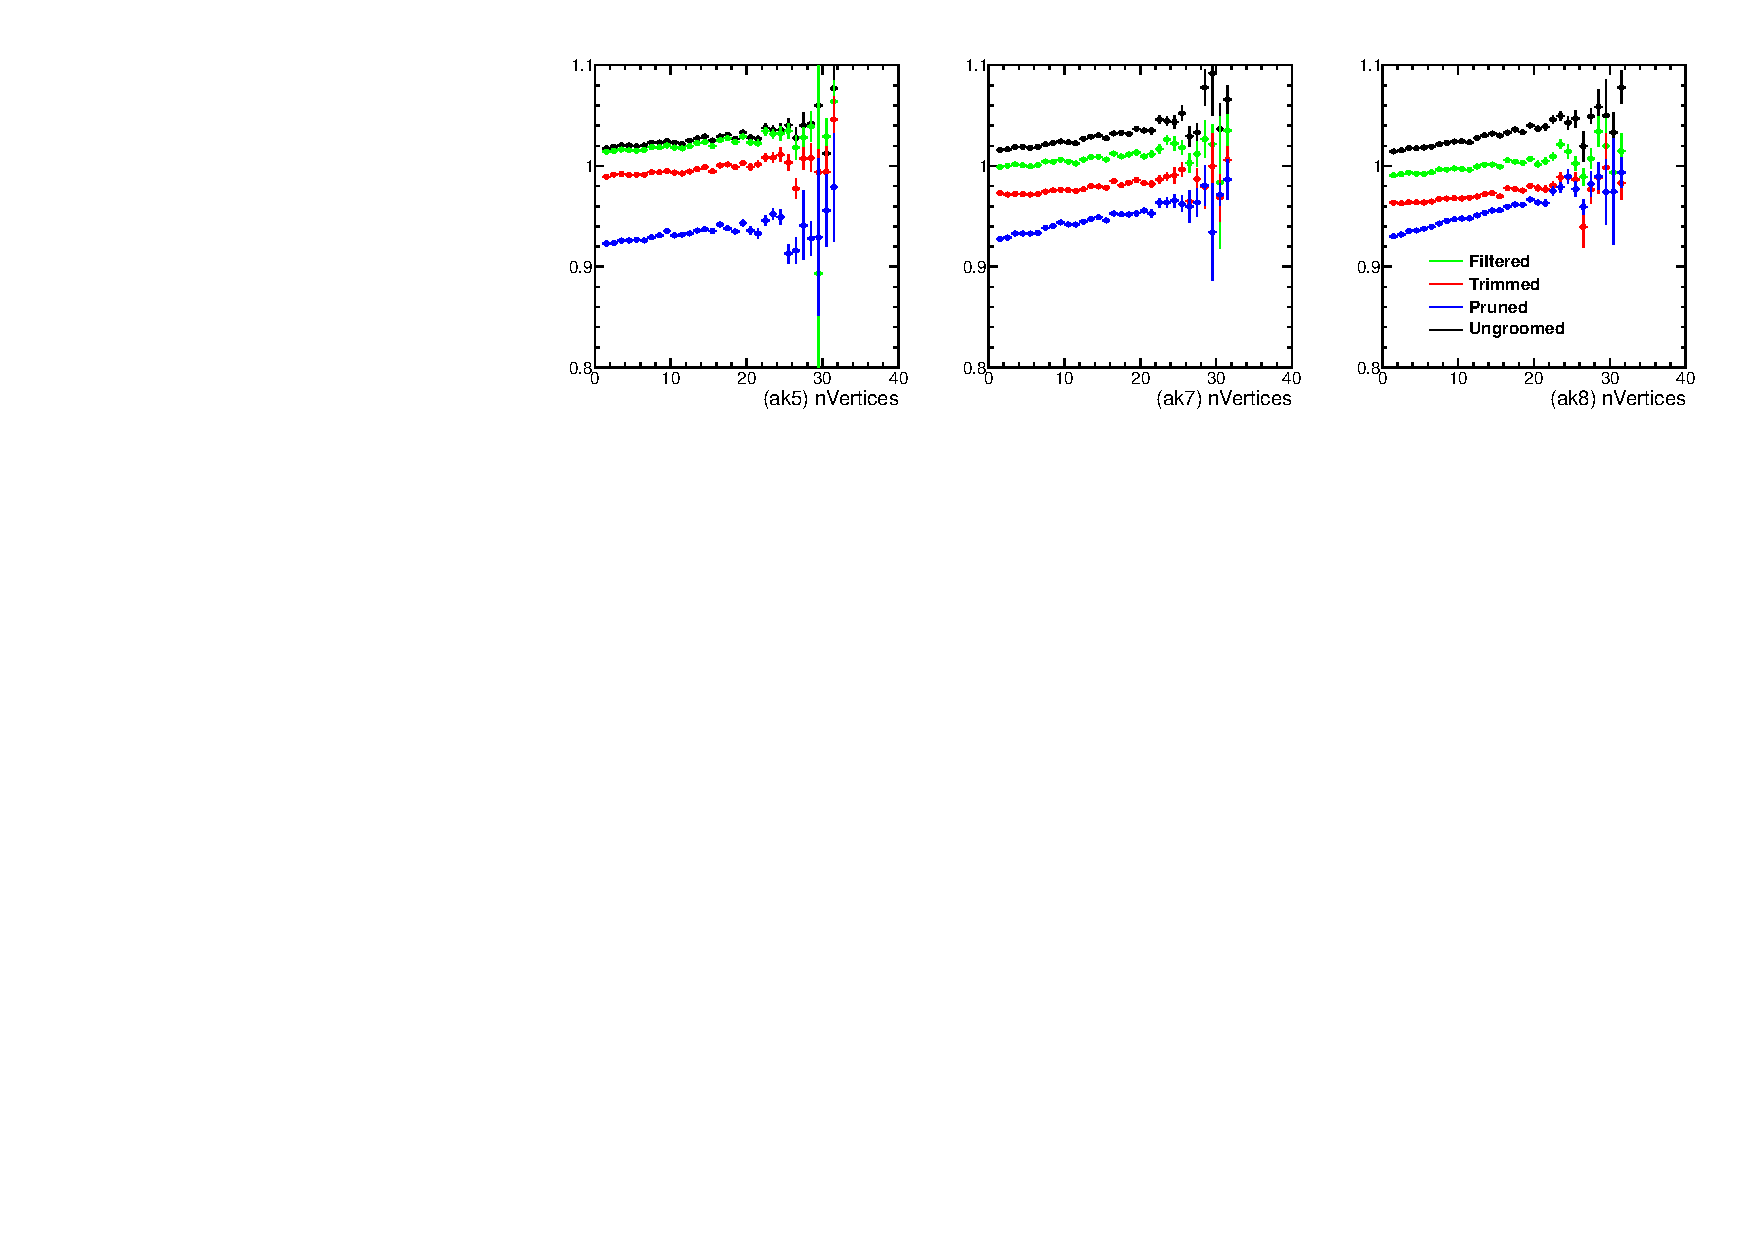
\includegraphics[width=1.0\textwidth]{figs/ptRatioVsNV_mean.pdf}
\caption{Jet response for different jet algorithms as a function of the primary vertex multiplicity in the event. Here, the
  substructure algorithms are compared to the
  generator-level AK5, AK7 and AK8 jets without the substructure algorithms applied.}
\label{figs:ptRatiovsPV}
\end{figure}


We then look at the corresponding resolution study for the jet mass. We first show the mass ratio dependence versus the jet momentum. Fig.~\ref{figs:massRatio} shows the ratio of the reconstructed  (ungroomed or groomed) jet mass over the ungrooomed generator  AK5, AK7 and AK8 jets. 

\begin{figure}[!htb]
\centering
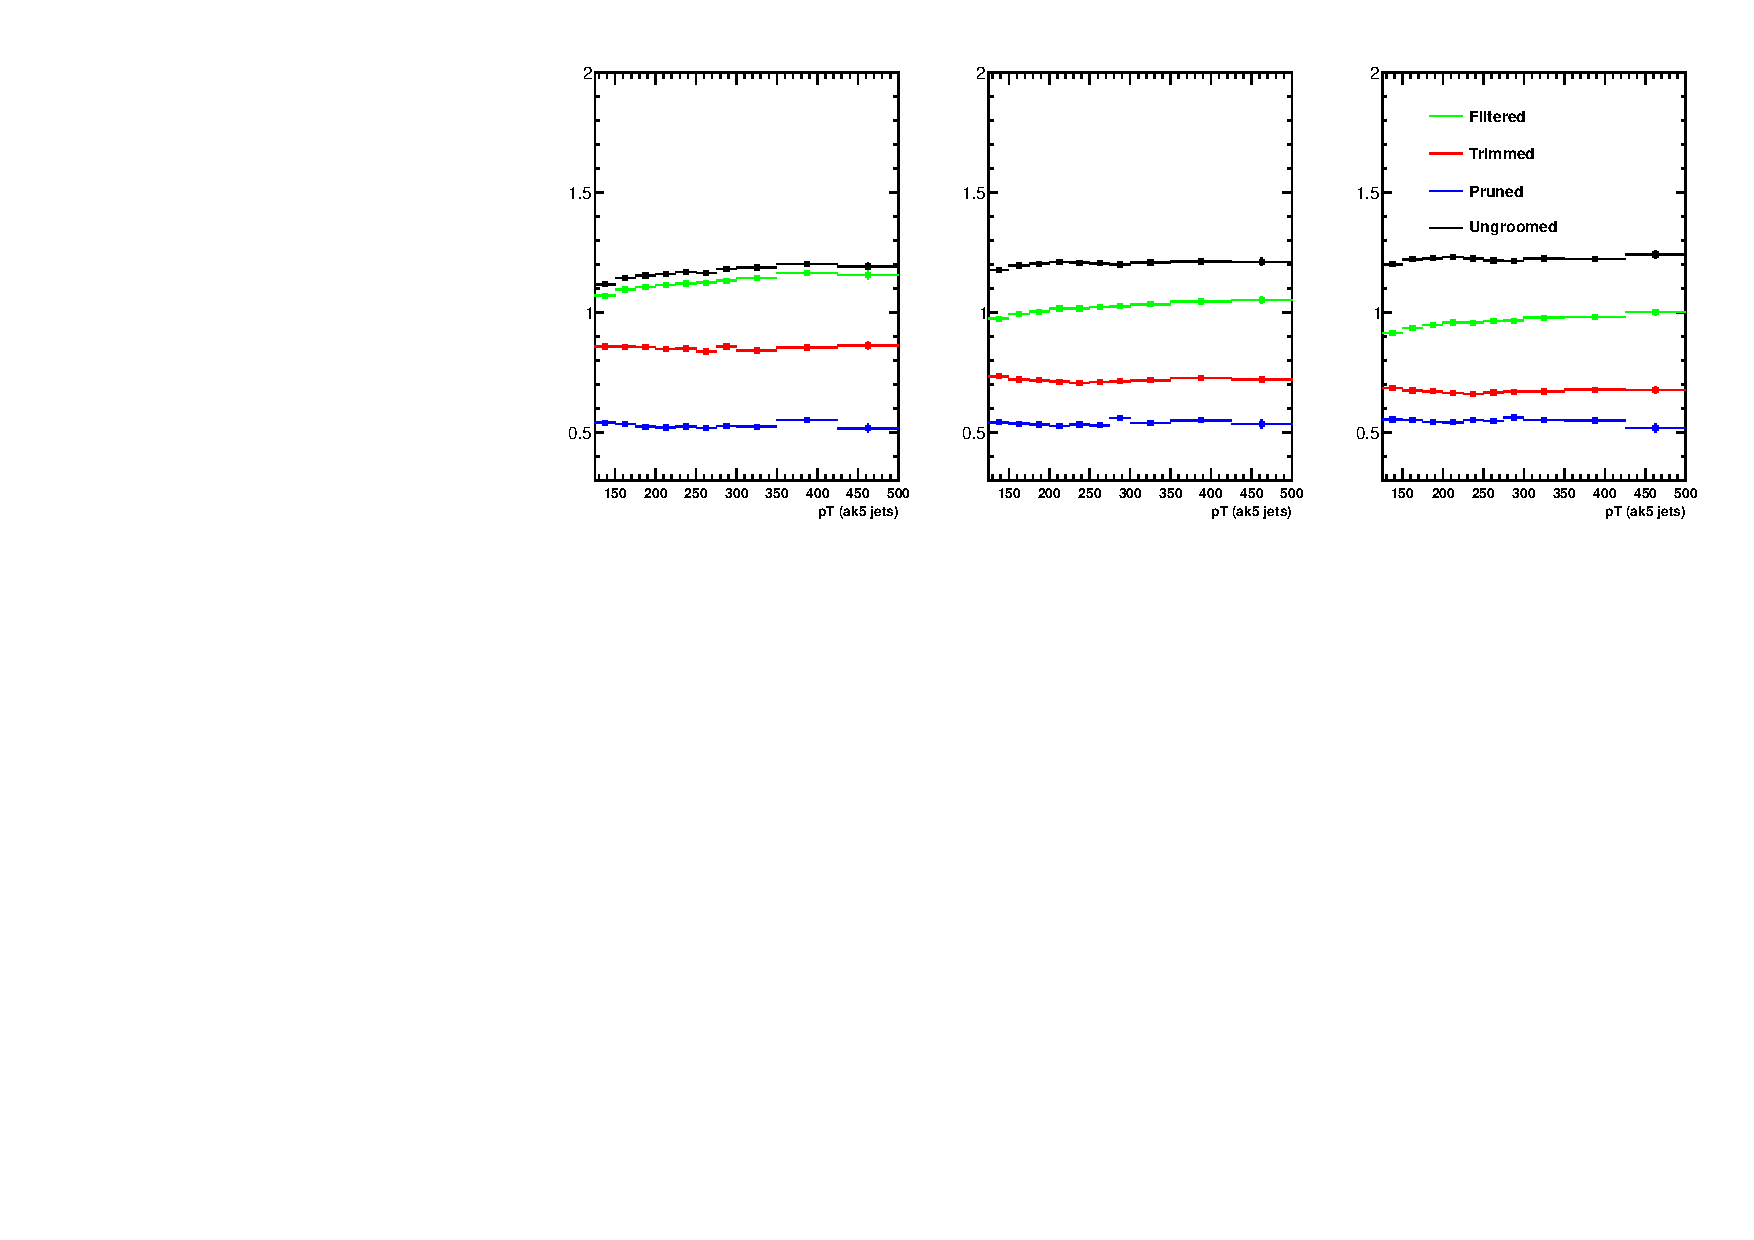
\includegraphics[width=1.0\textwidth]{figs/massRatioOvGen_vsPt.pdf}
\caption{Jet mass ratio for different jet algorithms as a function of the jet momentum. Here, the  substructure algorithms are compared to the
  generator-level AK5, AK7 and AK8 jets without the substructure algorithms applied.}
\label{figs:massRatio}
\end{figure}

We notice several interesting effects. First of all, we don't observe a sizable $p_t$ dependence for any of the ungroomed or groomed algorithms, apart for modest effect at low $p_t$  in the AK5 jets. In the ungroomed case, where we compare with ungroomed generator level jets, we see that the reconstructed mass overestimates the generated one by up to 20\%. This is not surprising and simply states that the reconstructed  mass has spurious constituents fromn the clustering process or PU residuals. The mass ratio for groomed jets becomes smaller and smaller the more aggressive the grooming is, up to the pruned jet where more than 40\% of the original ungroomed jet mass is removed by the pruning algorithm.  

Similar to the study above for the $p_T$ resolution, we then show the jet mass ratio  as a function of the jet pseudorapidity and the primary vertex multiplicity in fig.~\ref{figs:massRatiovsEta}-\ref{figs:massRatiovsNV}. No particular effect is seen in comparing the groomed jet behaviour with the ungroomed one.  

\begin{figure}[!htb]
\centering
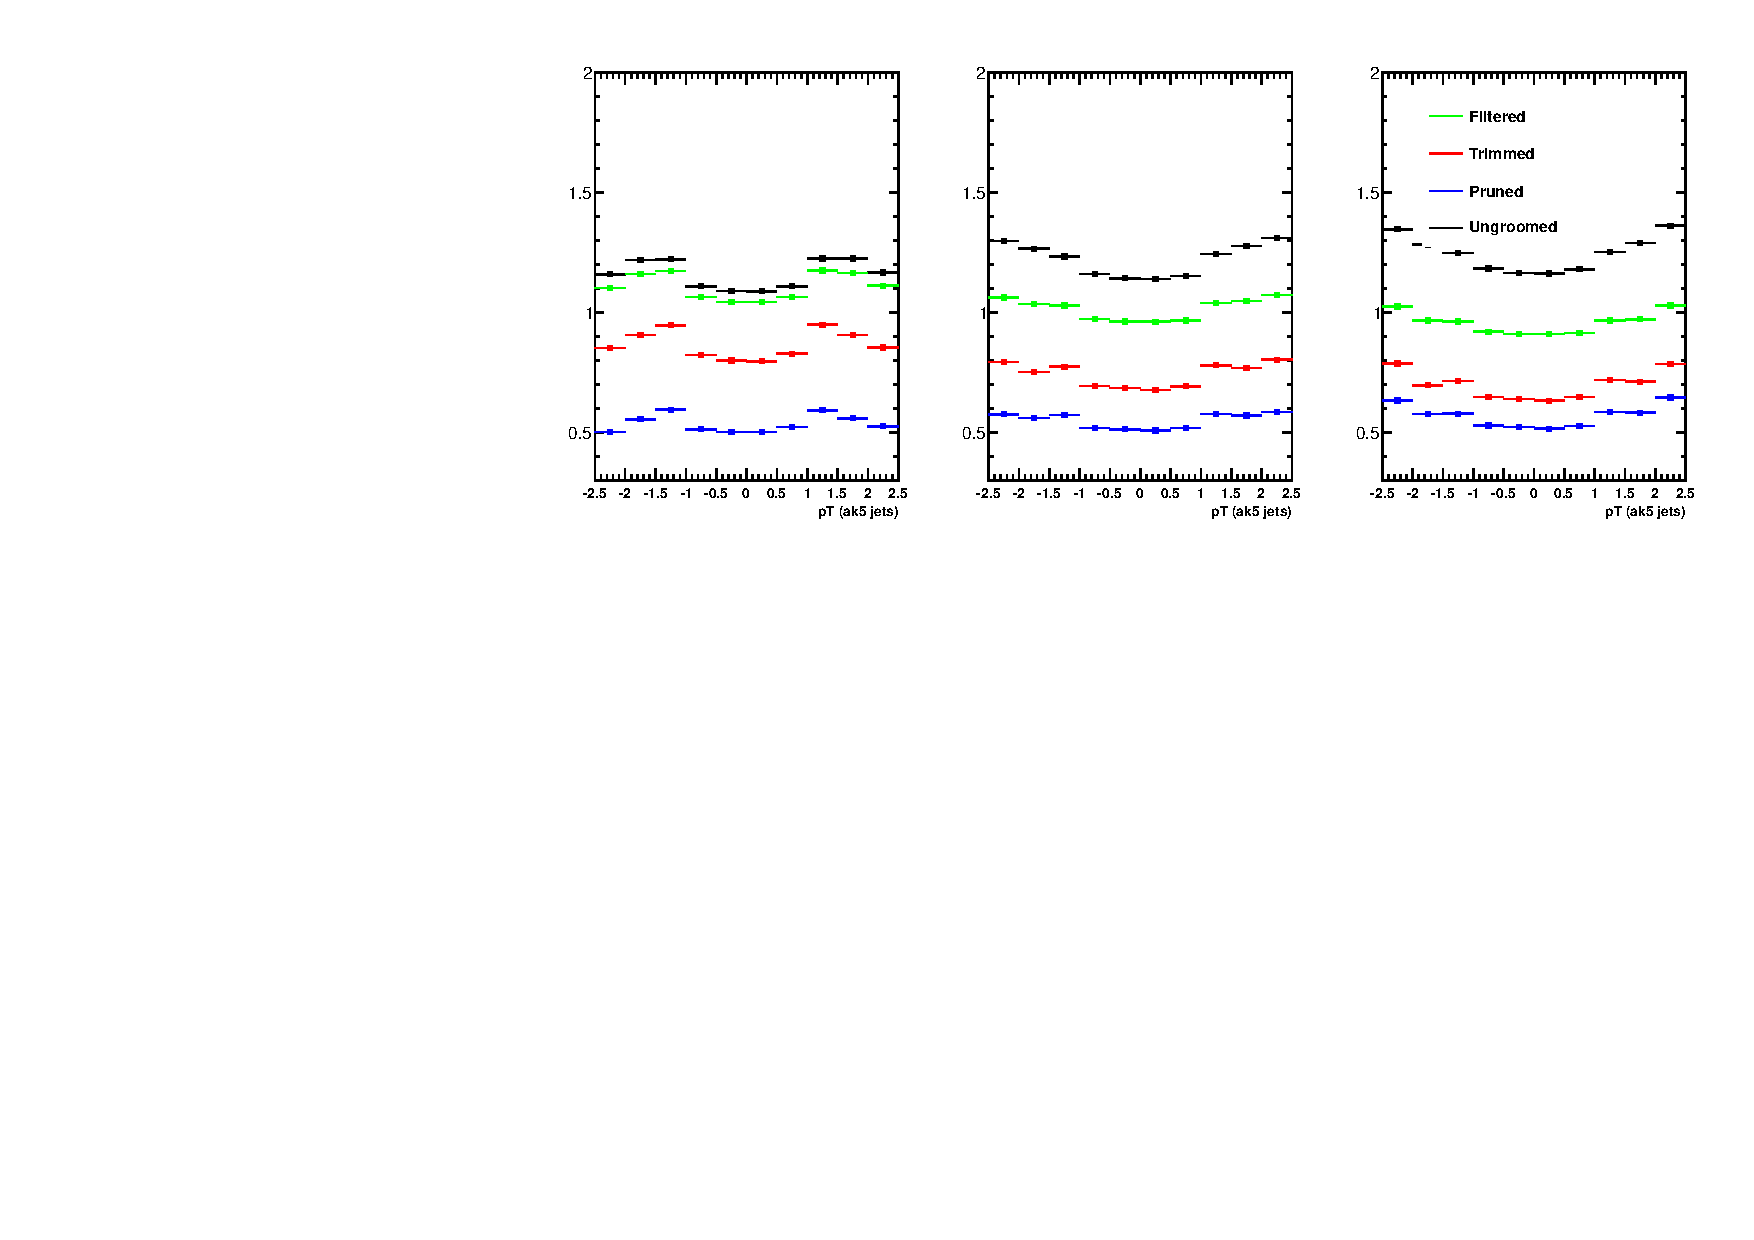
\includegraphics[width=1.0\textwidth]{figs/massRatioOvGen_vsEta.pdf}
\caption{Jet mass ratio for different jet algorithms as a function of the jet pseudorapidity. Here, the substructure algorithms are compared to the
  generator-level AK5, AK7 and AK8 jets without the substructure algorithms applied.}
\label{figs:massRatiovsEta}
\end{figure}

\begin{figure}[!htb]
\centering
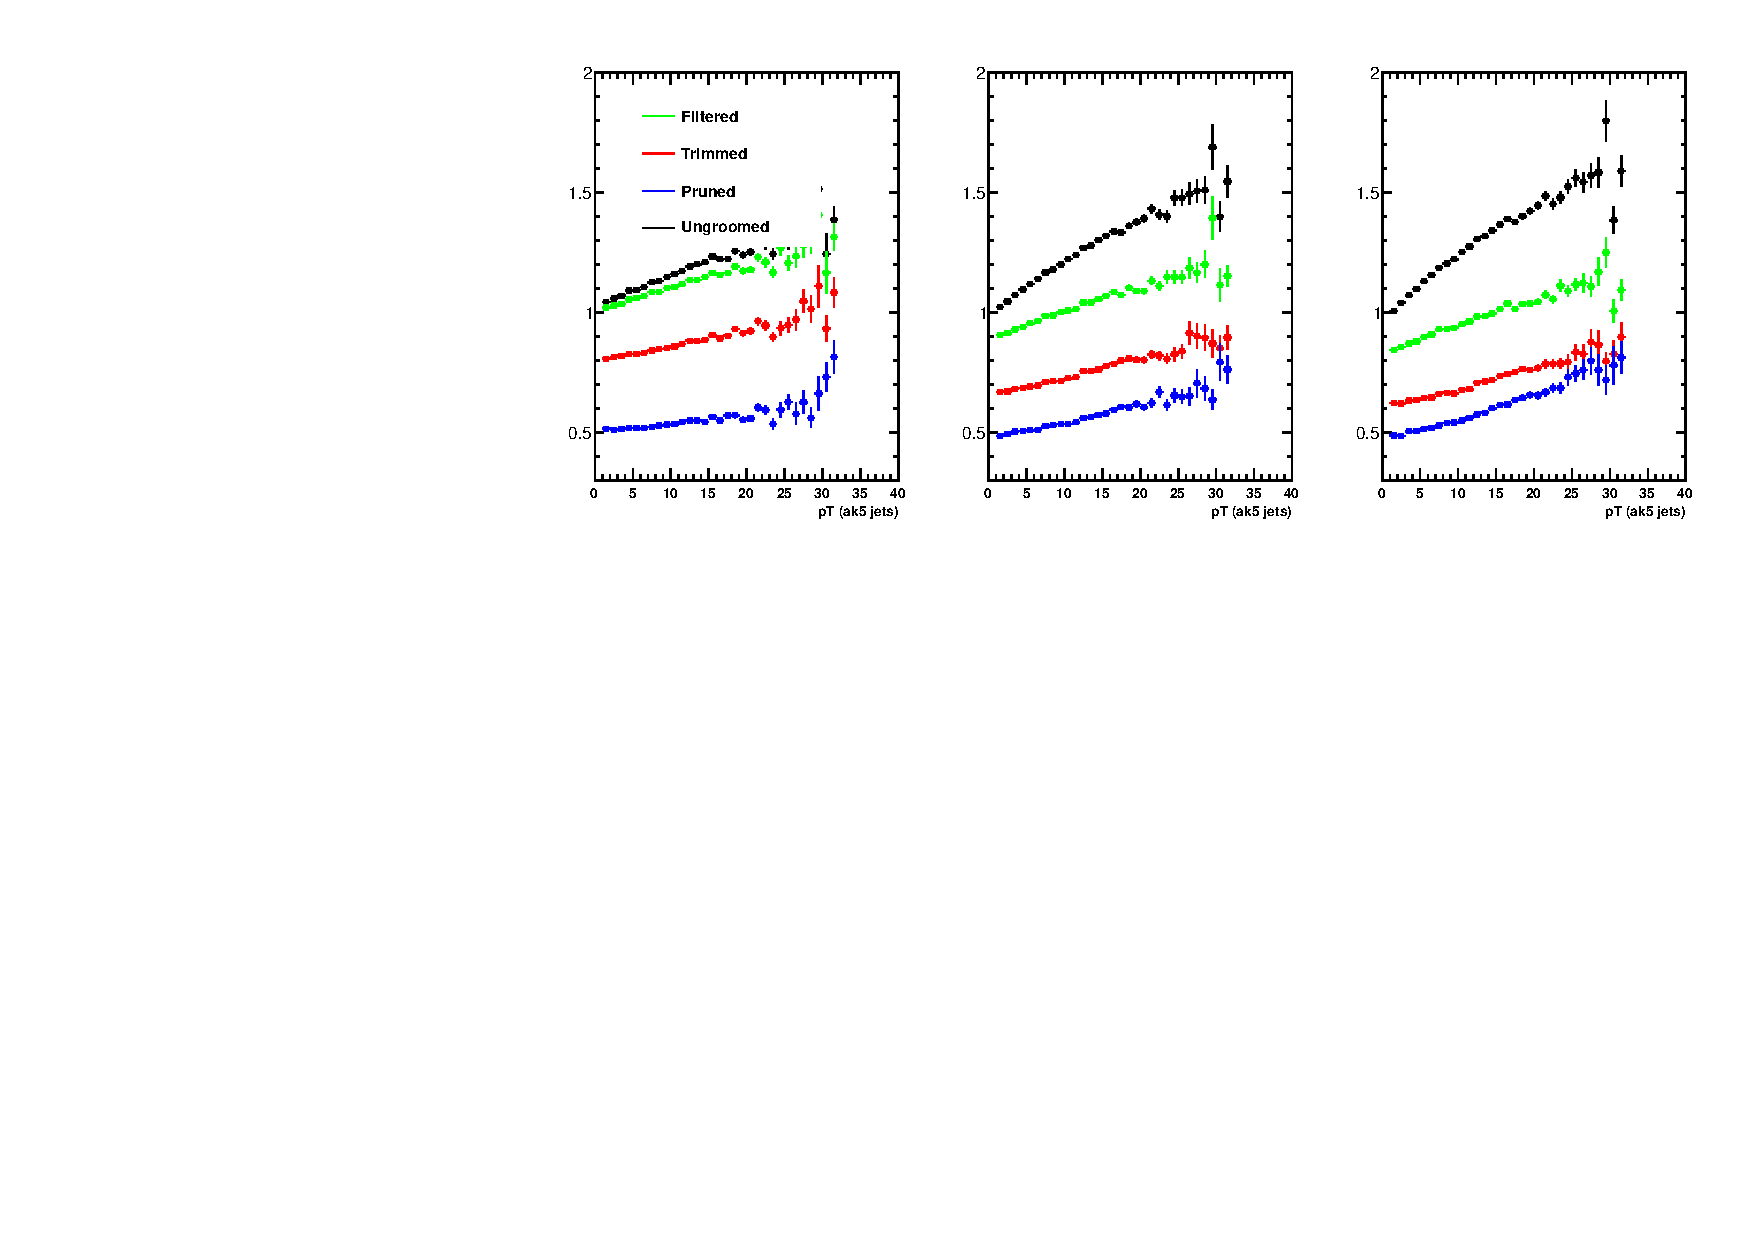
\includegraphics[width=1.0\textwidth]{figs/massRatioOvGen_vsNV.pdf}
\caption{Jet mass ratio for different jet algorithms as a function of the primary vertex multiplicity in the event. Here, the  substructure algorithms are compared to the
  generator-level AK5, AK7 and AK8 jets without the substructure algorithms applied.}
\label{figs:massRatiovsNV}
\end{figure}


In the jet mass ratio distributions considered so far we have compared the reconstructed (groomed or ungroomed) jet mass with the ungroomed generated one. We can now look at the same ratio using the reconstructed jet mass, i.e. measuring the ratio $(mass_{groomed} - mass_{ungroomed})/mass_{ungroomed}$. Fig.~\ref{figs:massRatioData} shows this ratio as a function of the jet momentum in data and MC events.

\begin{figure}[!htb]
\centering
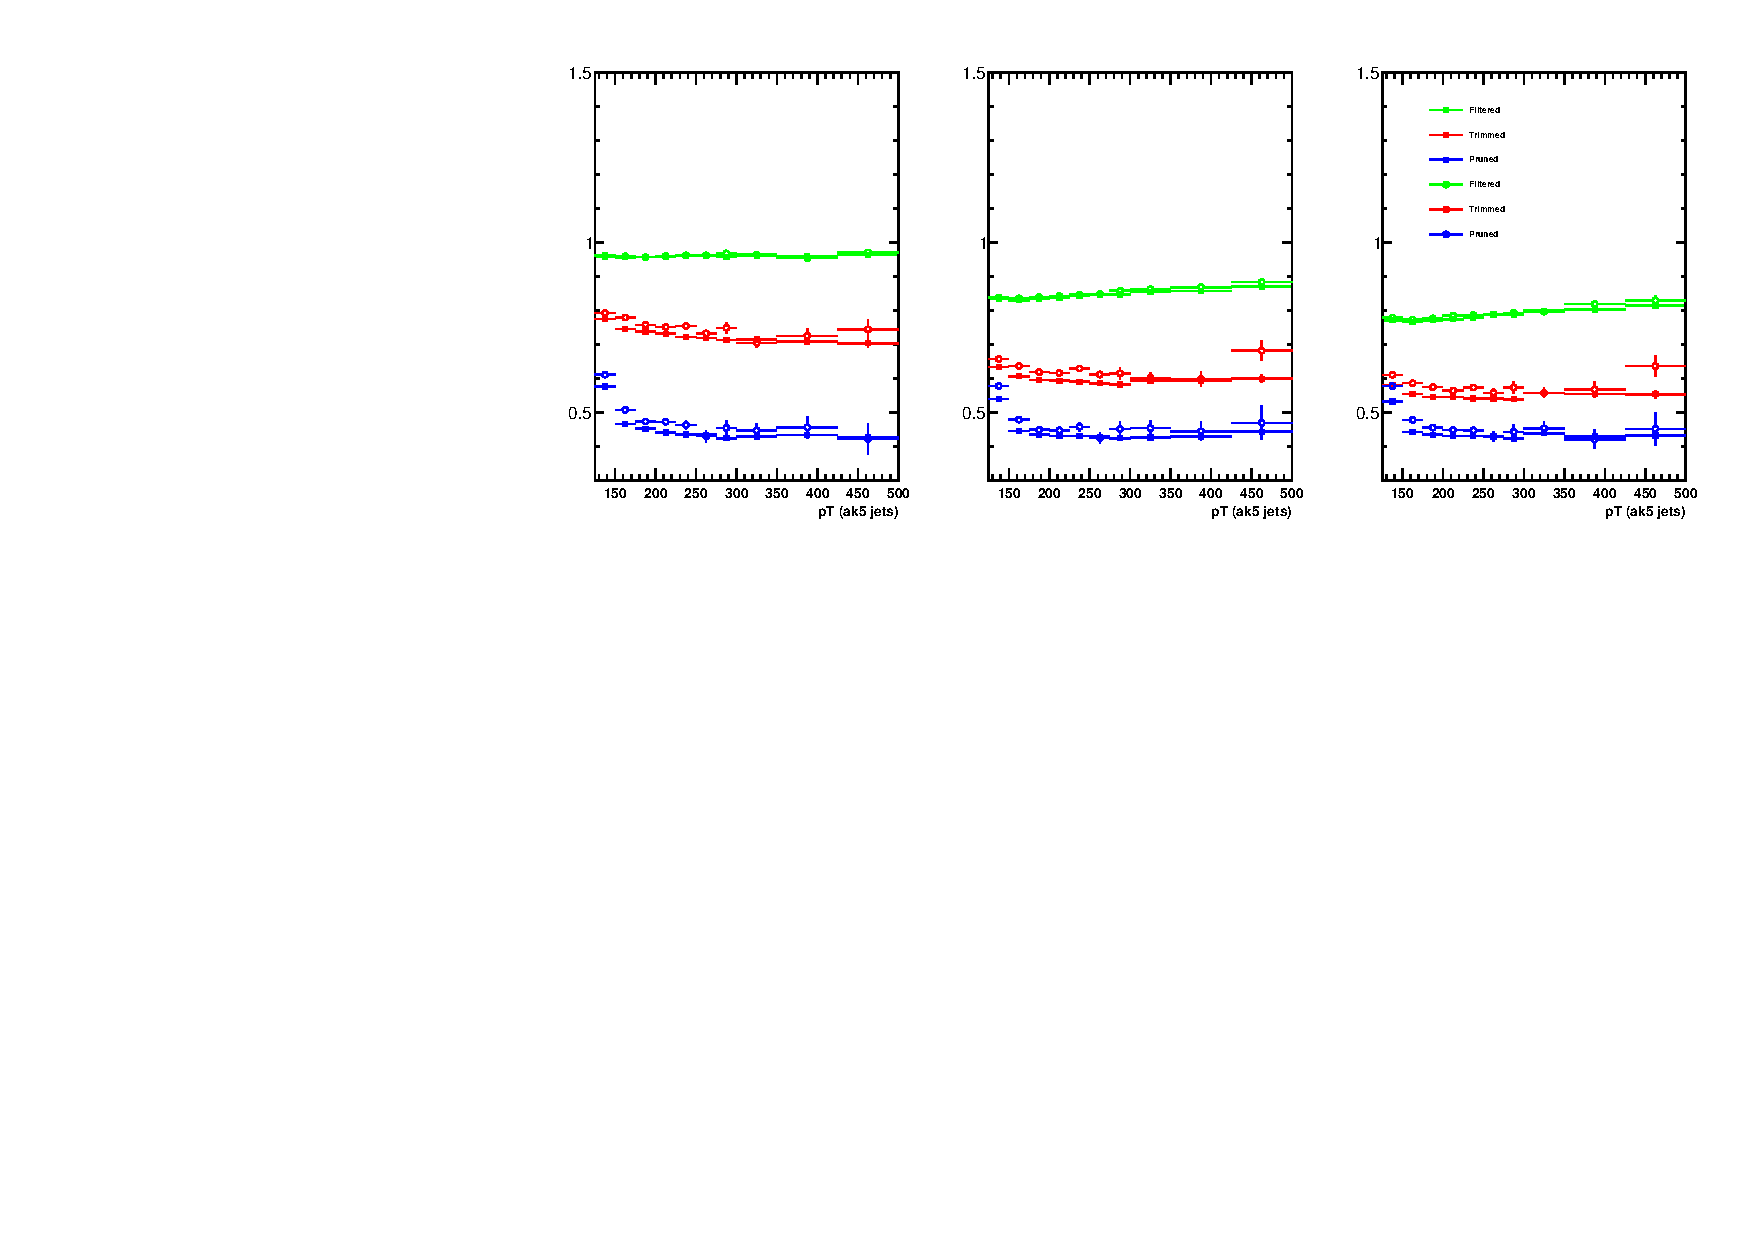
\includegraphics[width=1.0\textwidth]
{figs/massRatioOvReco_vsPt.pdf}
\caption{Reconstructed Jet mass ratio for different jet algorithms as a function of the jet momentum. 
Here, the substructure algorithms are compared to the
  reconstructed ungroomed AK5, AK7 and AK8 jets. Data: empty cicle, MC: filled square.}
\label{figs:massRatioData}
\end{figure}
     

%that have the same substructure algorithm applied as the reconstructed-level
%jets. That is, \verb!AK5PFJets! are compared to \verb!AK5GenJets! in both
%plots, \verb!CA8PFJets! are compared to \verb!CA8GenJets! in both plots,
%\verb!CA8PFJets! with top tagging are compared to \verb!CA8GenJets! with
t%op tagging, and \verb!CA8PFJets! with pruning are compared to \verb!CA8GenJets!
%with pruning. The top tagged jets (in purple) are directly above the ``bare''
%CA8 jets, because the algorithm does not modify the total jet.

% This shows us
%that the AK5 jet corrections are working as expected for the CA8 jets.
%The conservative 3\% systematic uncertainty we are applying in addition to the
%default uncertainties covers this effect.

%However, if the same procedure is applied to the generator-level jets,
%the agreement is much better, with a bias of 2\%. This means that the jet
%pruning algorithm is slightly more aggressive in the ``simulated data''
%than it is at the generator particle level.



\fi





\section{Unfolding procedure}
The unfolding procedure is exactly the same as in Ref.~\cite{cmsSMPJSVJ}. Here we discuss the unfolding
briefly for completeness. 

\subsection{Unfolding}
The measured spectrum of a physical observable, like the jet mass distribution, is usually distorted by	detector effects, such as finite resolution and limited acceptance. Moreover, in this analysis the chosen bin size is comparabl
e to the resolution, so there is a significant migration of events generated in one jet bin mass and ending up in a different bin of reconstructed jet mass. A comparison of the measured mass spectrum with that predicted at generato
r level requires that we remove these effects to obtain the true underlying mass spectrum. There are several possible ways to achieve the unfolding of detector effects on measured spectra, and examples can be found in \cite{unfold}
 and references therein. In this section we describe the unfolding method adopted in this analysis, which largely follows the technique proposed in \cite{agostini}. 
A physical quantity $\alpha$, distributed according to its probability density function $f(\alpha)$, cannot be measured perfectly. Apart from statistical uncertainties, there will be effects from reconstruction efficiency and finite 
resolution of the detector. As	a result, instead of the true, physical variable $\alpha$, 
a variable $\beta$, distributed according to some distribution $g(\beta)$, is measured. 
The relation between $f(\alpha)$ and $g(\beta)$ can be expressed as a convolution of the 
true distribution $f(\alpha)$ with a kernel $\hat{A}(\alpha,\beta)$ describing the detector effects,

\begin{equation}
\int f(\alpha) \hat{A}(\alpha,\beta)d\alpha = g(\beta)
\end{equation}

\noindent The spectrum we intend to unfold is given as an histogram. Hence, we use vectors and matrices for the formulation of the convolution,	

\begin{equation}
\hat{A} x = b
\label{eq:unf1}
\end{equation}

\noindent where the $i$-th component of the $n_x$-dimensional vector $x$ and the $n_b$-dimensional vector $b$ contain the number of entries in bin $i$ of the true and the measured distribution, respectively. 
$\hat{A}$ is a $(n_b - n_x)$-dimensional matrix, and contains the detector effects. An event with a true value in bin $j$ might be measured with a value in bin $i$ (i.e. finite resolution) or might not be measured at all. The matri
x element $\hat{A}_{ij}$ represents the probability for an event	 with a true value in bin $x_j$ to be measured with a value in bin $b_i$.
Assuming that the measurement process is well simulated, $\hat{A}$ can be determined on Monte Carlo events by tracking the true and reconstructed values for each event. A well-defined system of linear equations is obtained,

\begin{equation}
\hat{A} x^{ini} = b^{ini}
\end{equation}


\noindent where the index ``ini''denotes the use of Monte Carlo spectra $x^{ini}$ , $b^{ini}$. Technically, the matrix element $\hat{A}_{ij}$ is determined by taking the number of events that fall into bin $j$ of $x^{ini}$ and at t
he same time into bin $i$ of $b^{ini}$, and by dividing this number by the number of events in bin $j$ of $x^{ini}$.

Now that $\hat{A}$ is determined and we have a measured spectrum $b$, one can try to solve Eq.~\ref{eq:unf1} for the true spectrum $x$. However, the apparently easiest way to determine $x$, i.e. applying $x = \hat{A}^{-1}b$, is not
 adequate. Even when $\hat{A}$ can be inverted, statistical fluctuations in the measured spectrum introduce spurious, non-physical oscillations in the solution for $x$. Therefore a more efficient method needs to be applied. 

We use an unfolding procedure described by G.~D.~Agostini in~\cite{agostini}. Repeated application of Bayes theorem is used to invert the response matrix. Regularization is achieved by stopping iterations before reaching the ``true
'' (but wildly fluctuating) inverse. The regularization parameter is just the number of iterations.
 In principle, this has to be tuned to prevent the statistical fluctuations being interpreted as structure in the true distribution, according to the sample statistics and binning. In practice, the results are fairly insensitive to
 the precise setting used and four iterations are usually sufficient.
The training truth is taken as its initial prior, rather than a flat distribution. This should not bias result once we have iterated, but could reach an optimum after fewer iterations.
This implementation takes account of errors on the data sample but not, by default, uncertainties in the response matrix due to finite MC statistics. That calculation can be very slow, and usually the training sample is much larger
 than the data sample.
%RooUnfoldBayes does not normally do smoothing, since this has not been found to be necessary 2
%and can, in principle, bias the distribution. Smoothing can be enabled with an option.

\ifnpas
The {\tt RooUnfold} package~\cite{roounfold} has been used with the {\tt RooUnfoldBayes} class,
with the number of iterations set to four. 
\fi

\subsection{Response matrices}

The detector response matrix for the different jet clustering algorithms are showed in Fig.~\ref{figs:response_QCD_pythia6_z2_plots_nominal_ptall}-\ref{figs:response_QCD_herwigpp_23_plots_nominal_Pruned_ptall}. 
We show the response in the nine nominal $p_T$ bins used for the analysis, for the AK7 jets with the 
following clustering algorithm: ungroomed, pruned, filtered and trimmed.
In the response matrix derivation, the appropriate physical $\pt$ weighting is
used. If one uses the unphysical flat-$\pt$ spectrum, this introduces
unphysical biases in the tails of the jet mass distribution. 



\begin{figure}[htbp]
\centering
\subfigure{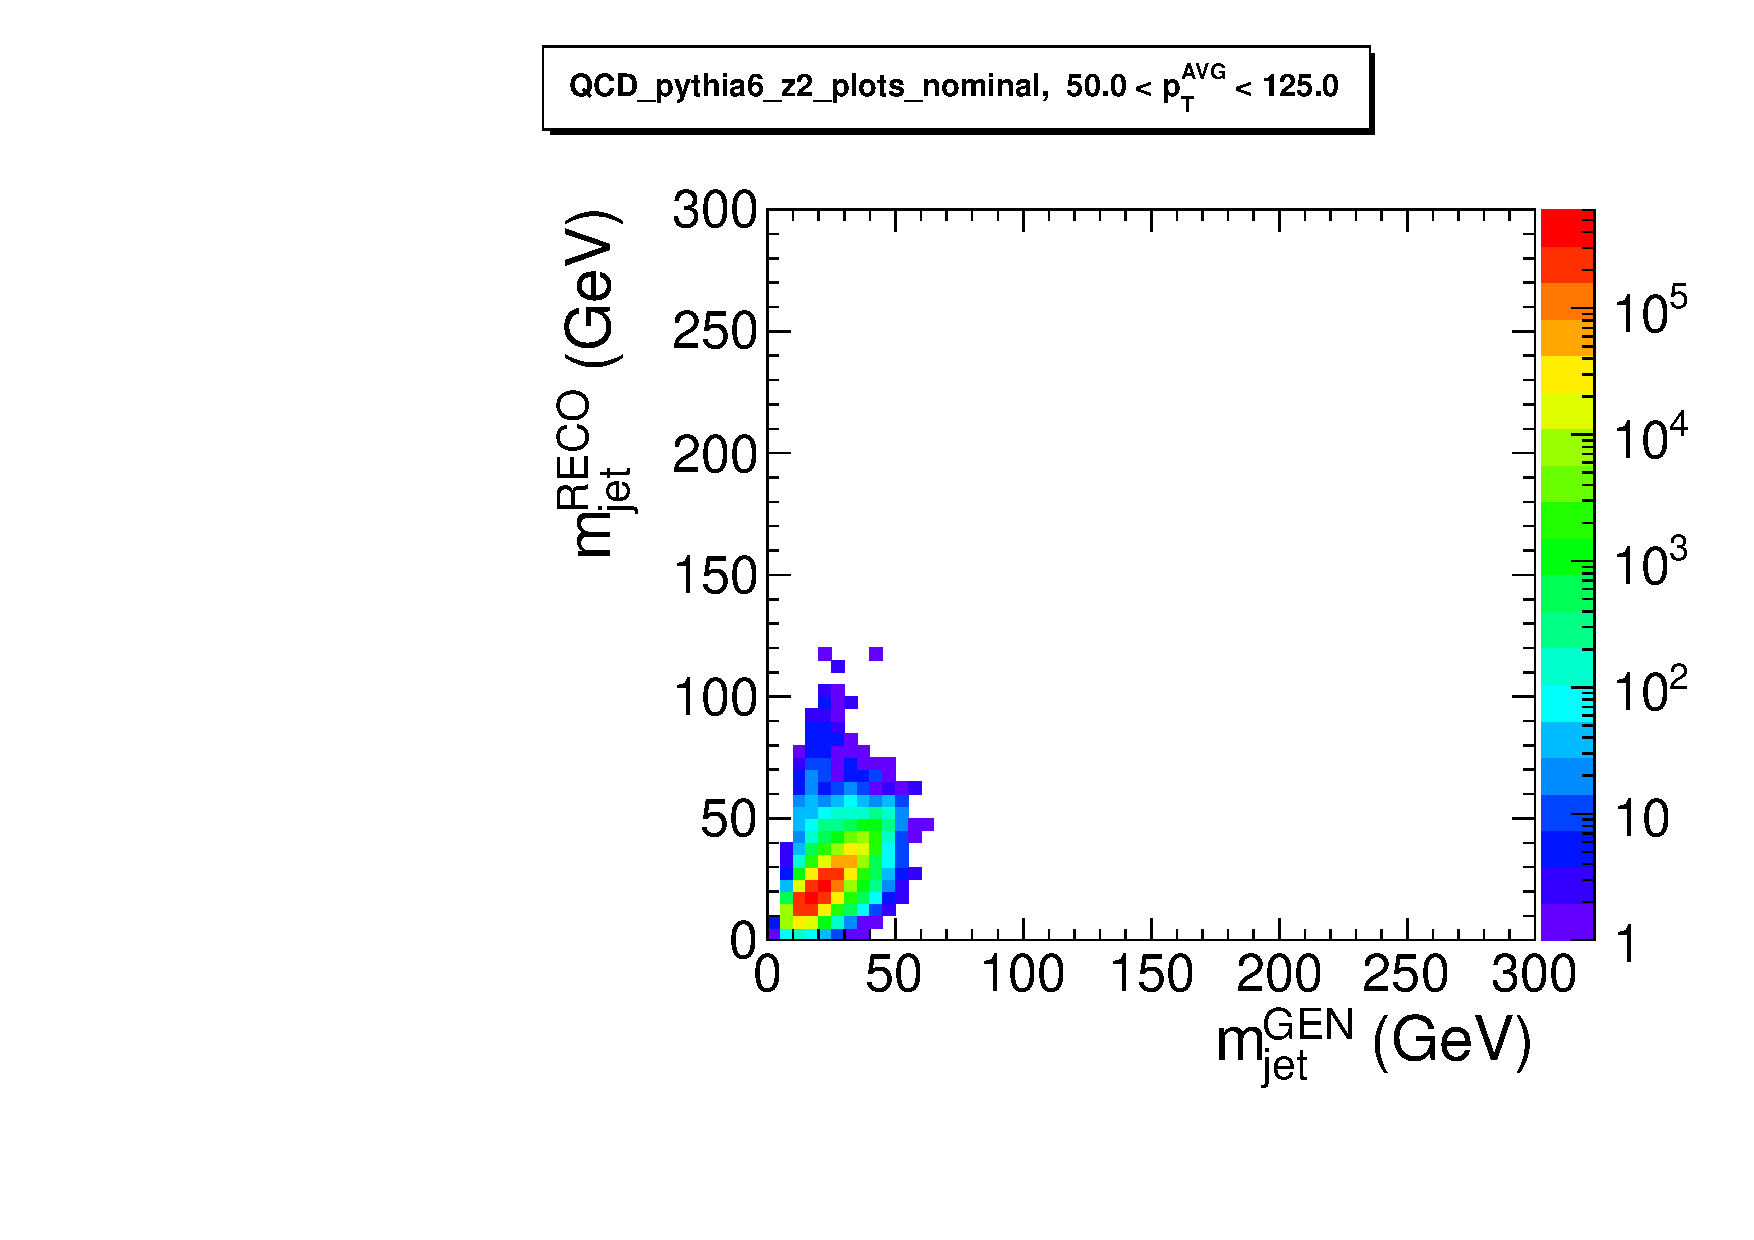
\includegraphics[width=0.3\textwidth]{figs/response_QCD_pythia6_z2_plots_nominal_pt1}}
\subfigure{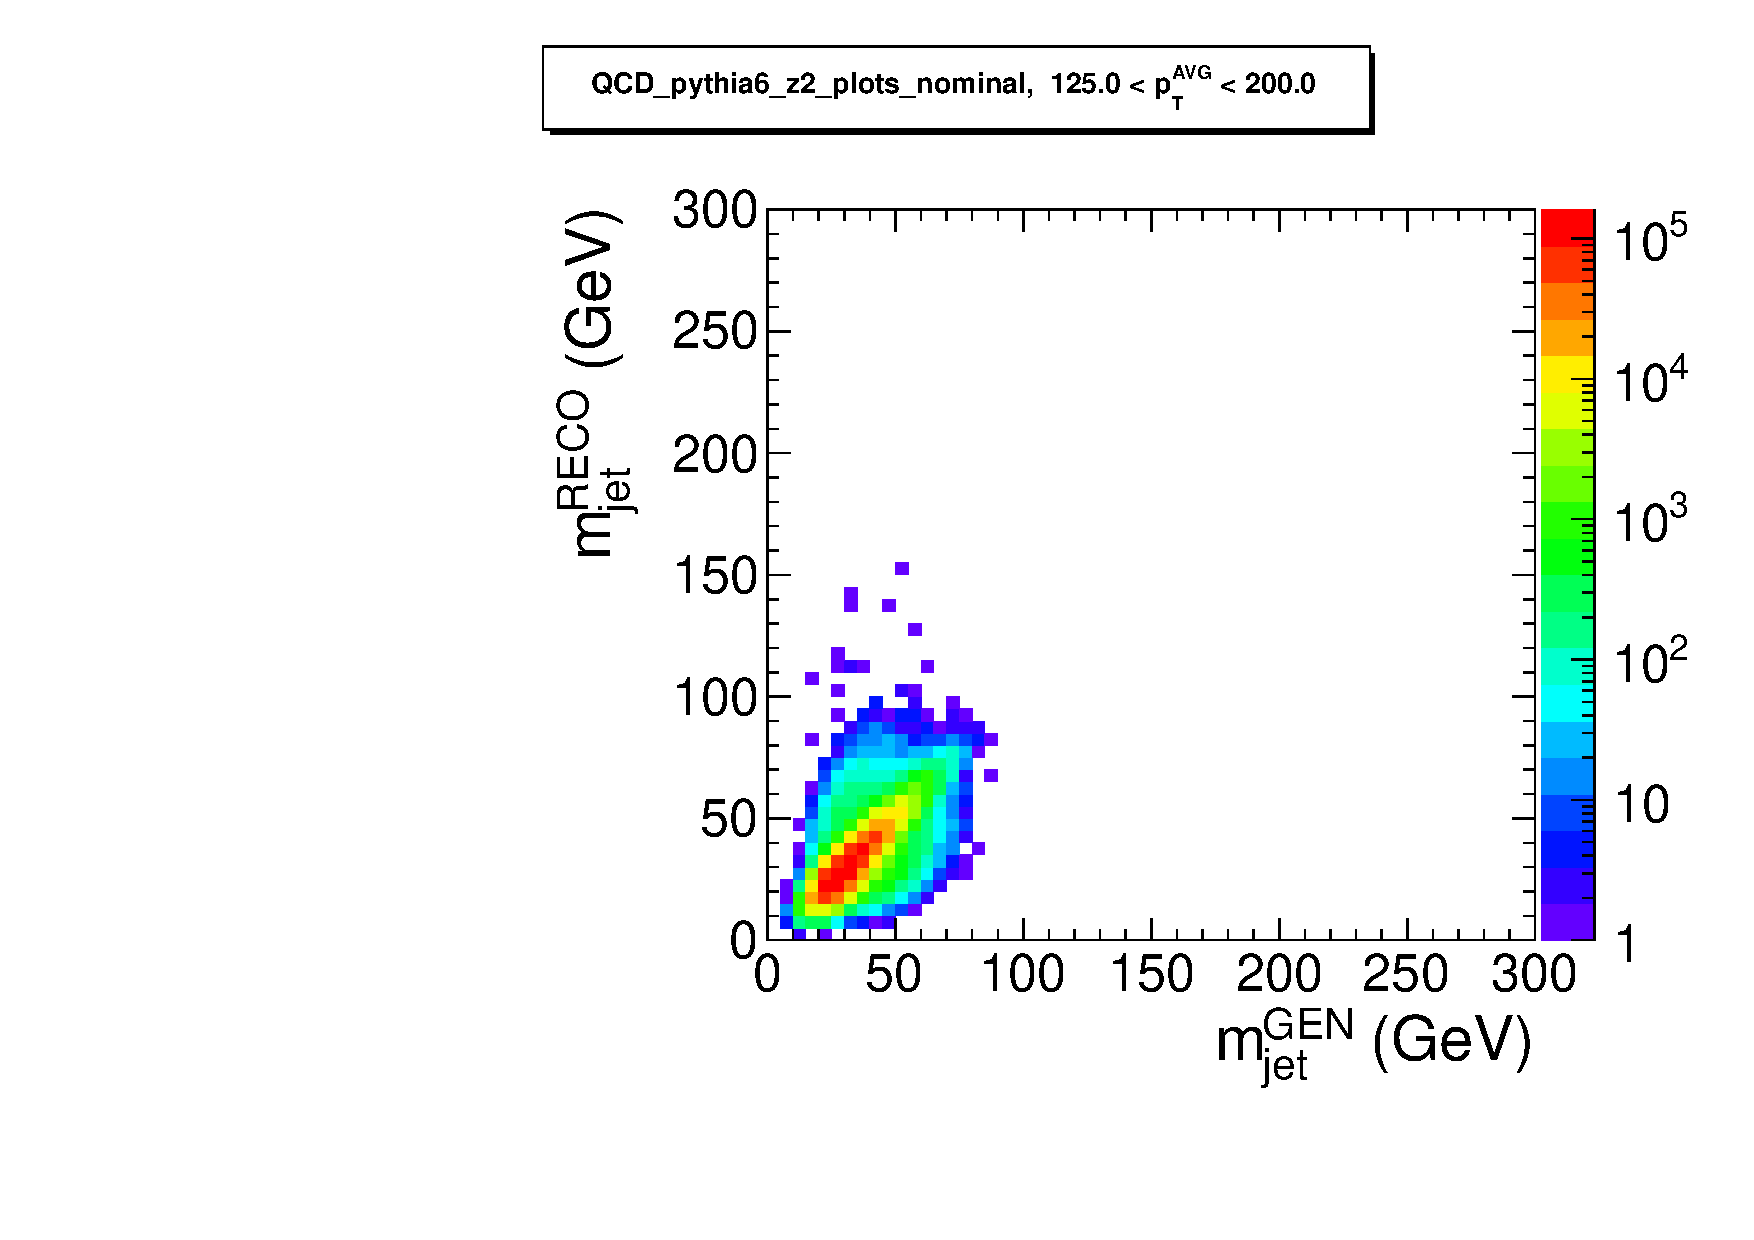
\includegraphics[width=0.3\textwidth]{figs/response_QCD_pythia6_z2_plots_nominal_pt2}}
\subfigure{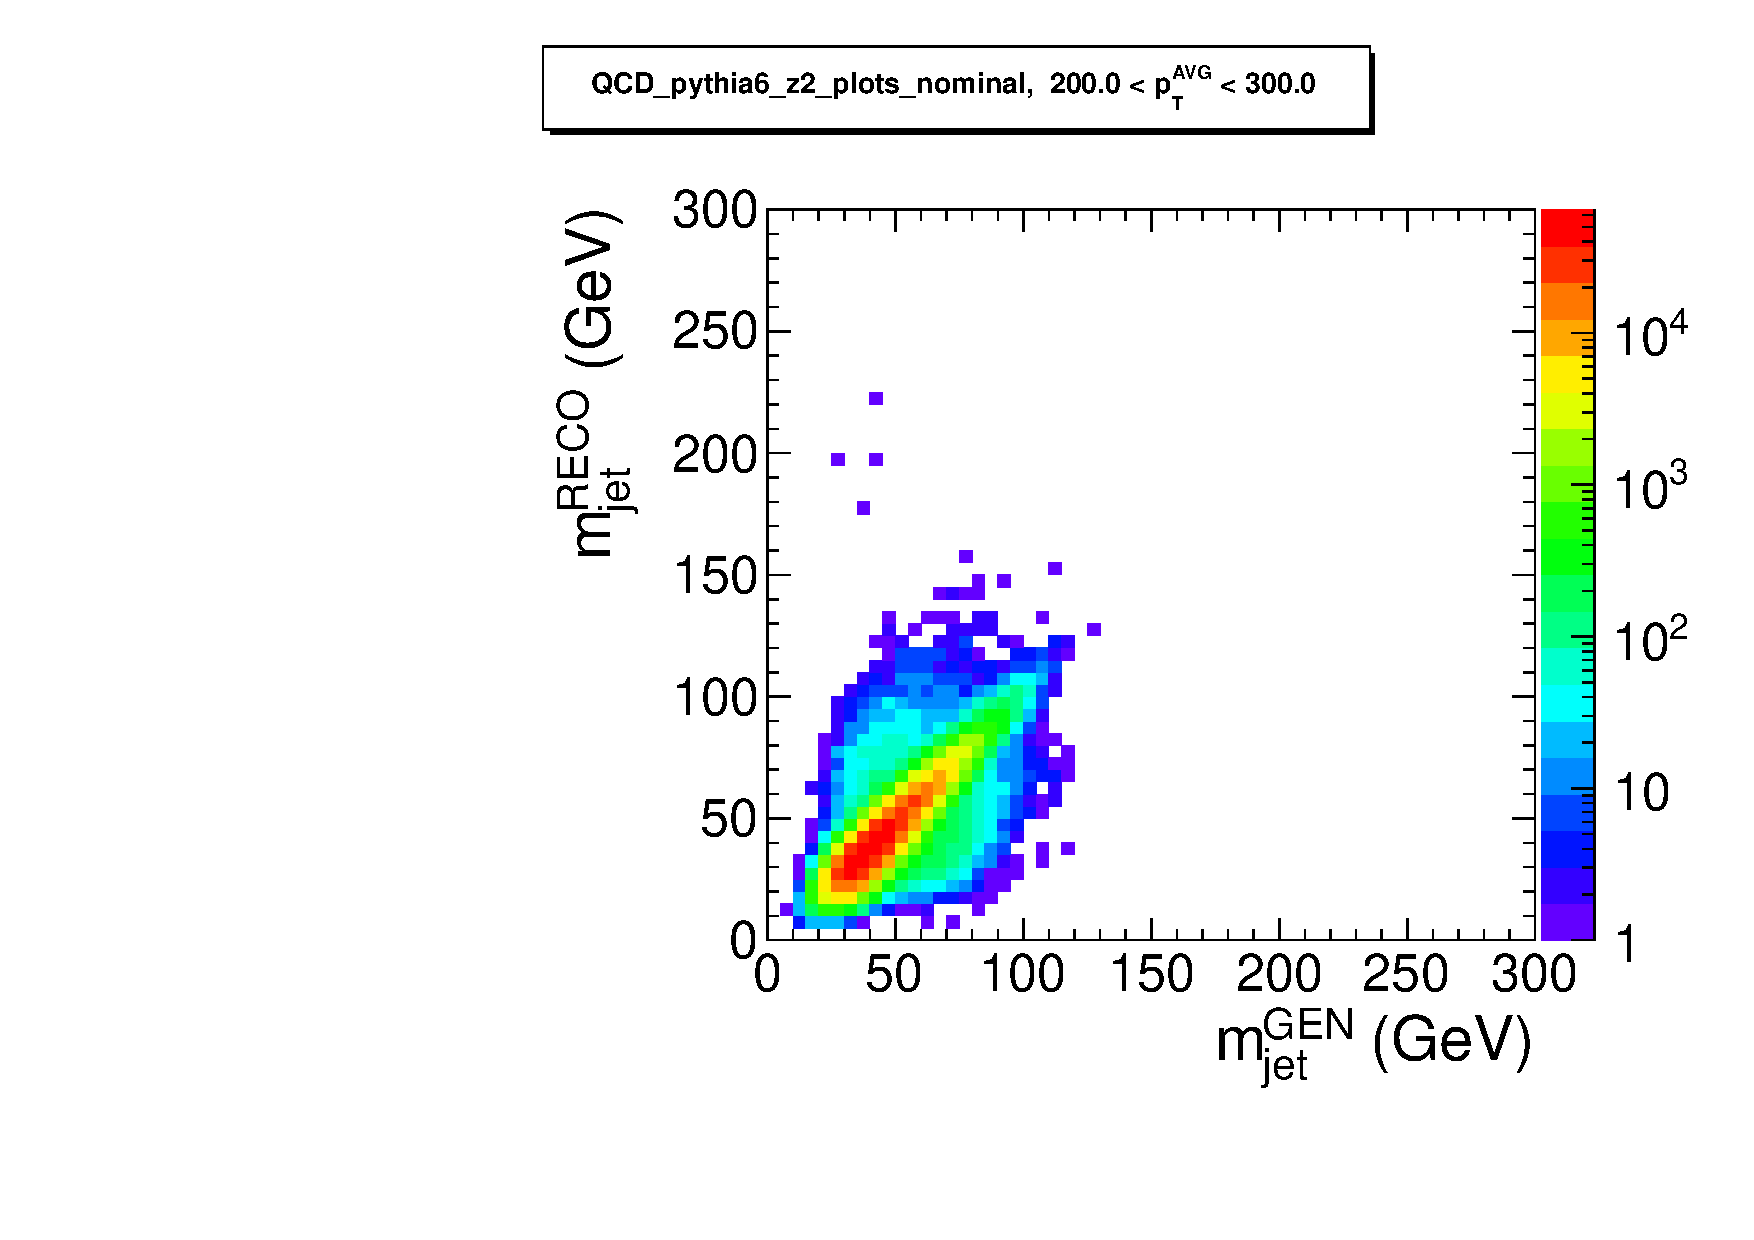
\includegraphics[width=0.3\textwidth]{figs/response_QCD_pythia6_z2_plots_nominal_pt3}}\\
\subfigure{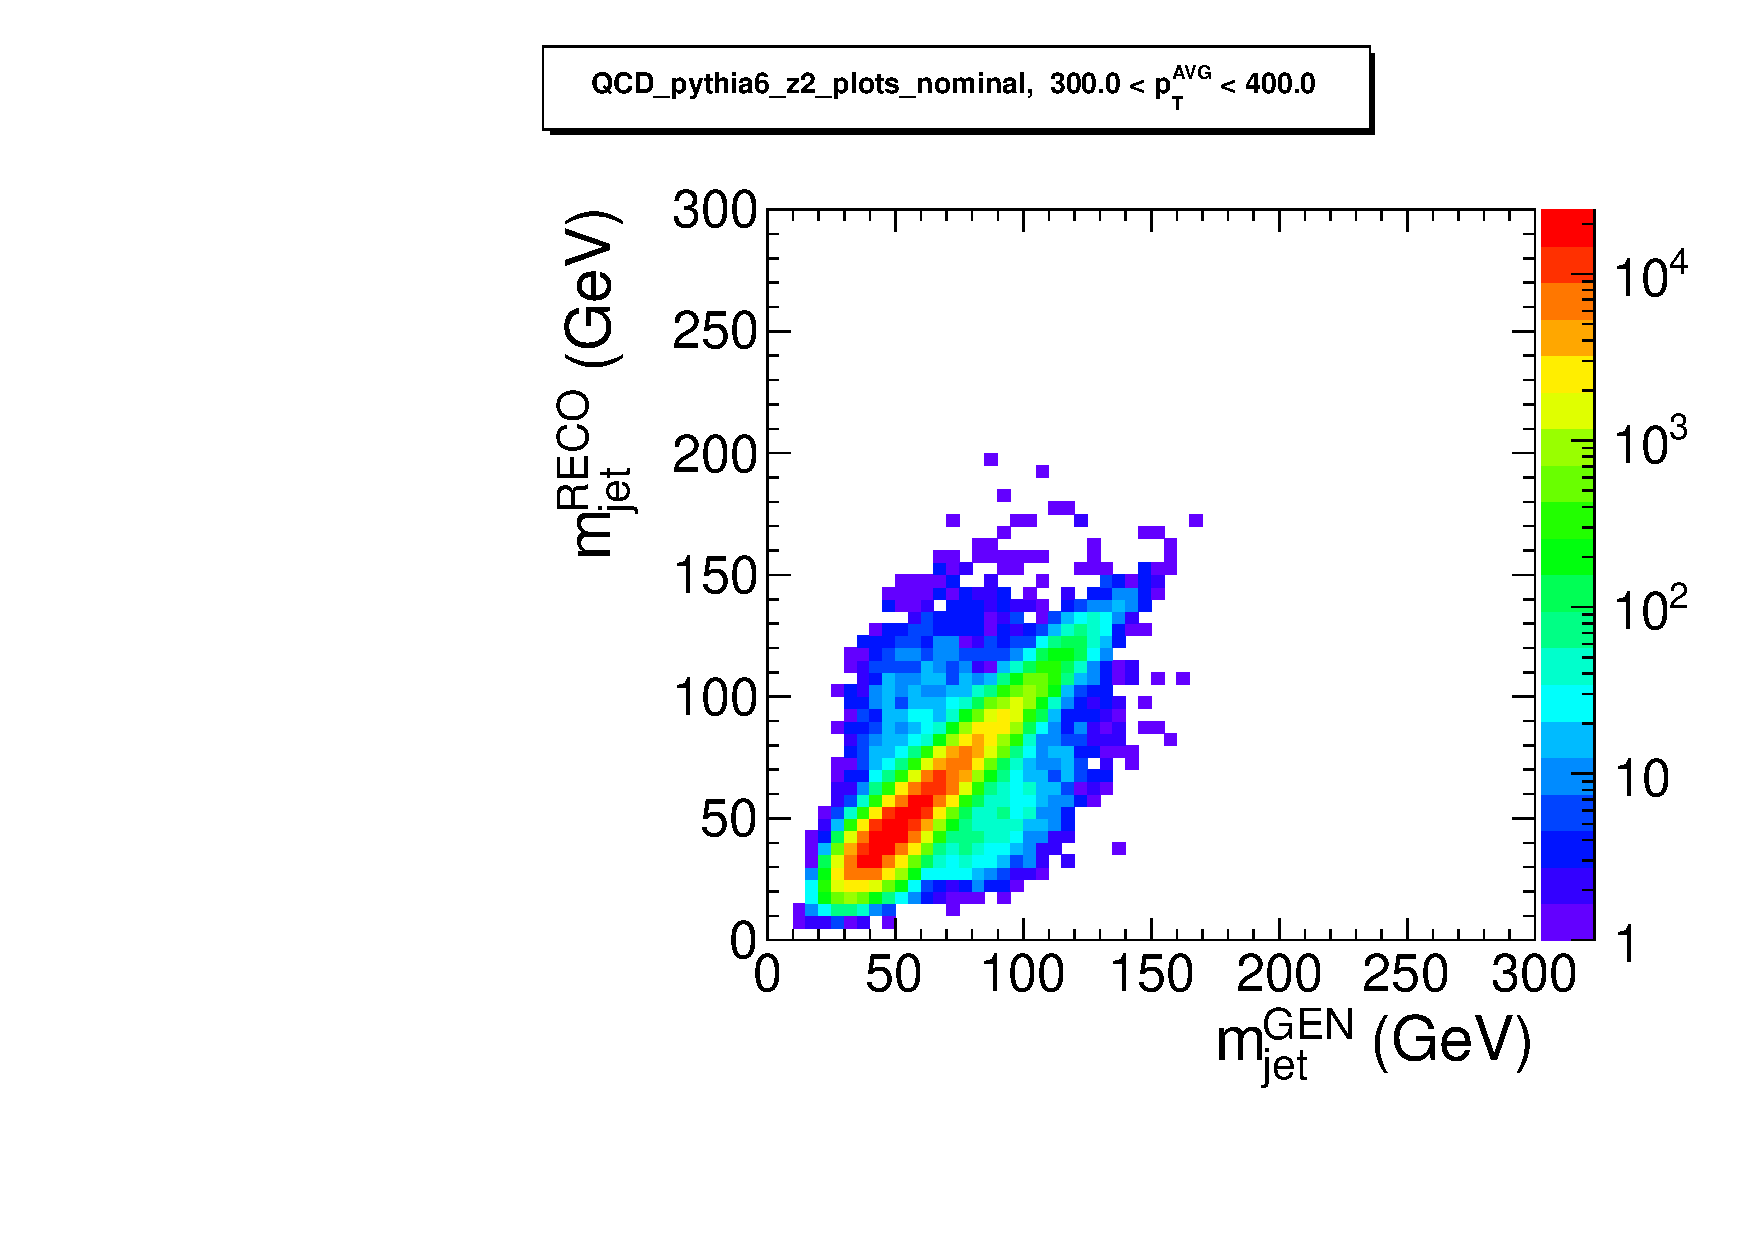
\includegraphics[width=0.3\textwidth]{figs/response_QCD_pythia6_z2_plots_nominal_pt4}}
\subfigure{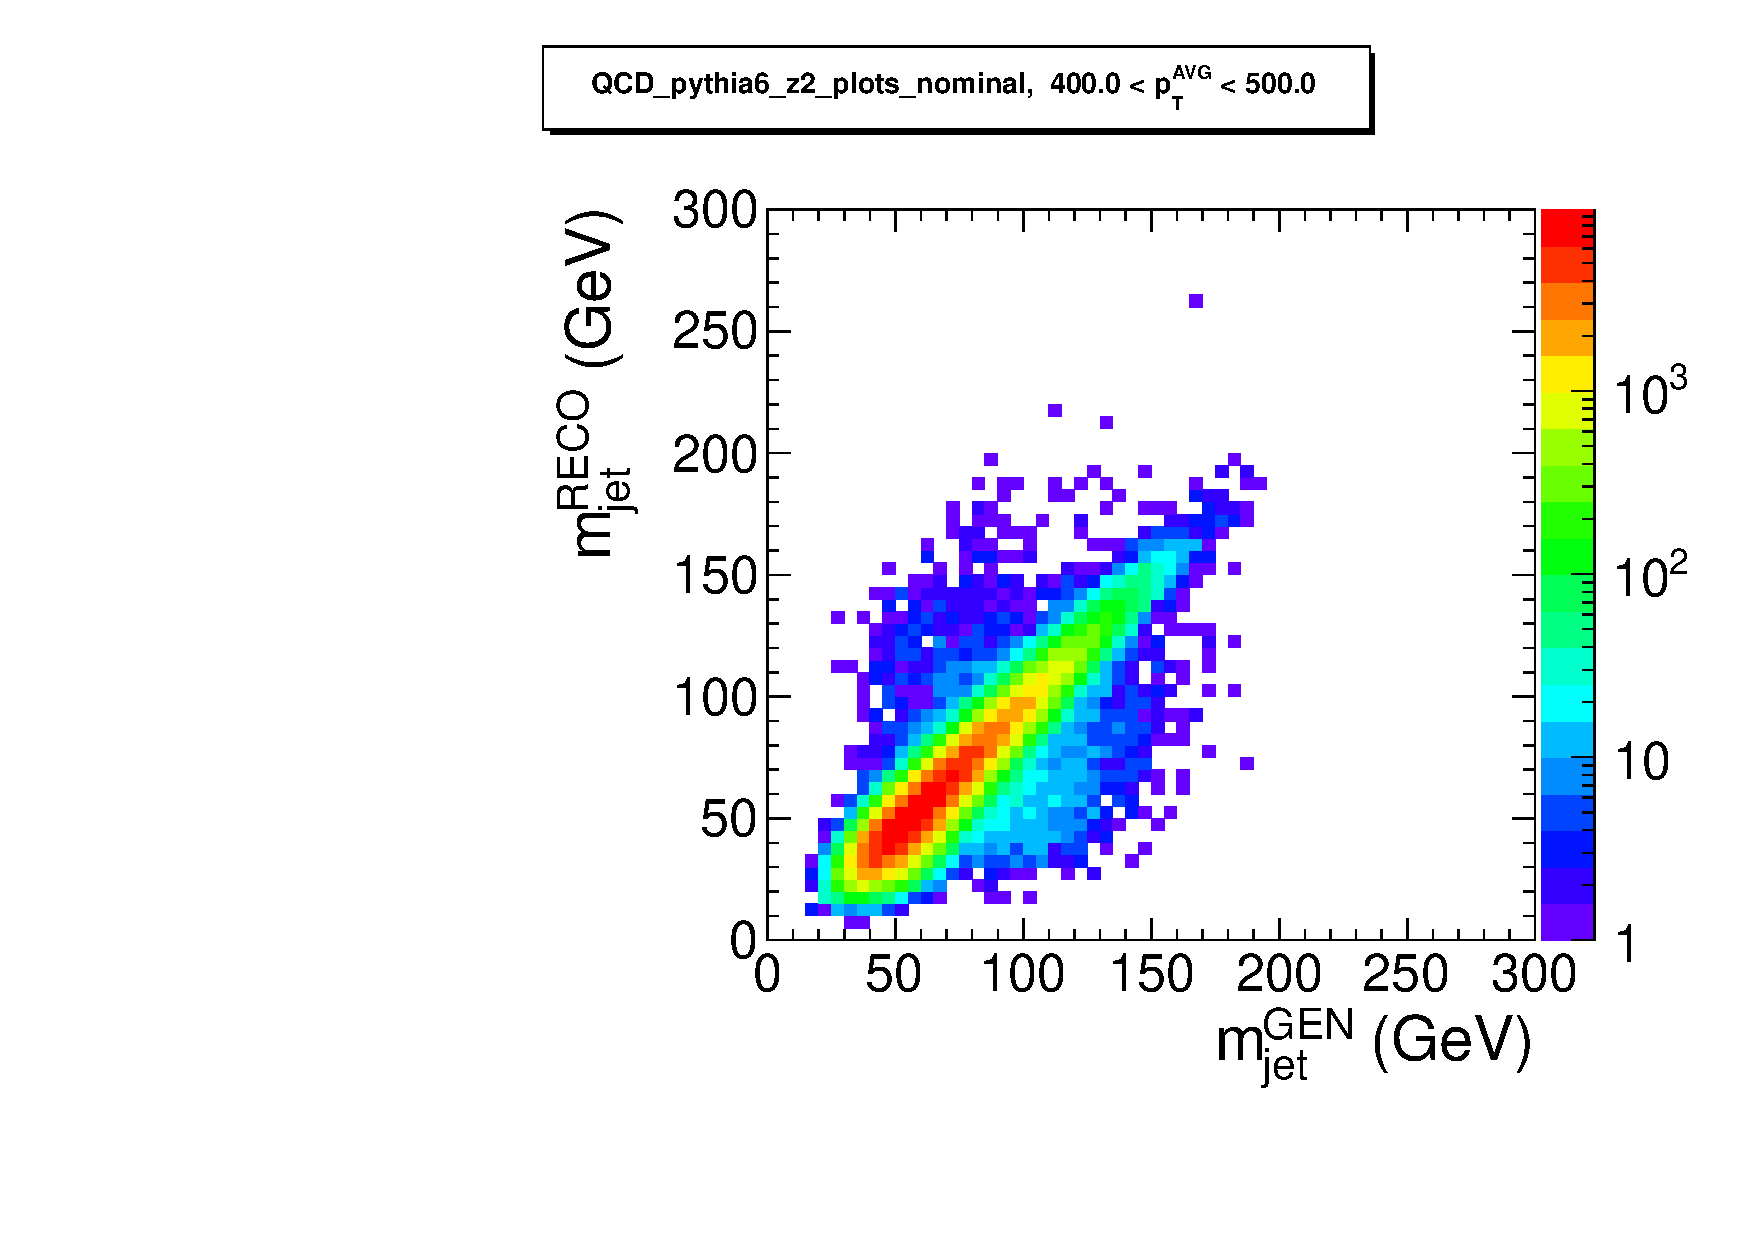
\includegraphics[width=0.3\textwidth]{figs/response_QCD_pythia6_z2_plots_nominal_pt5}}
\subfigure{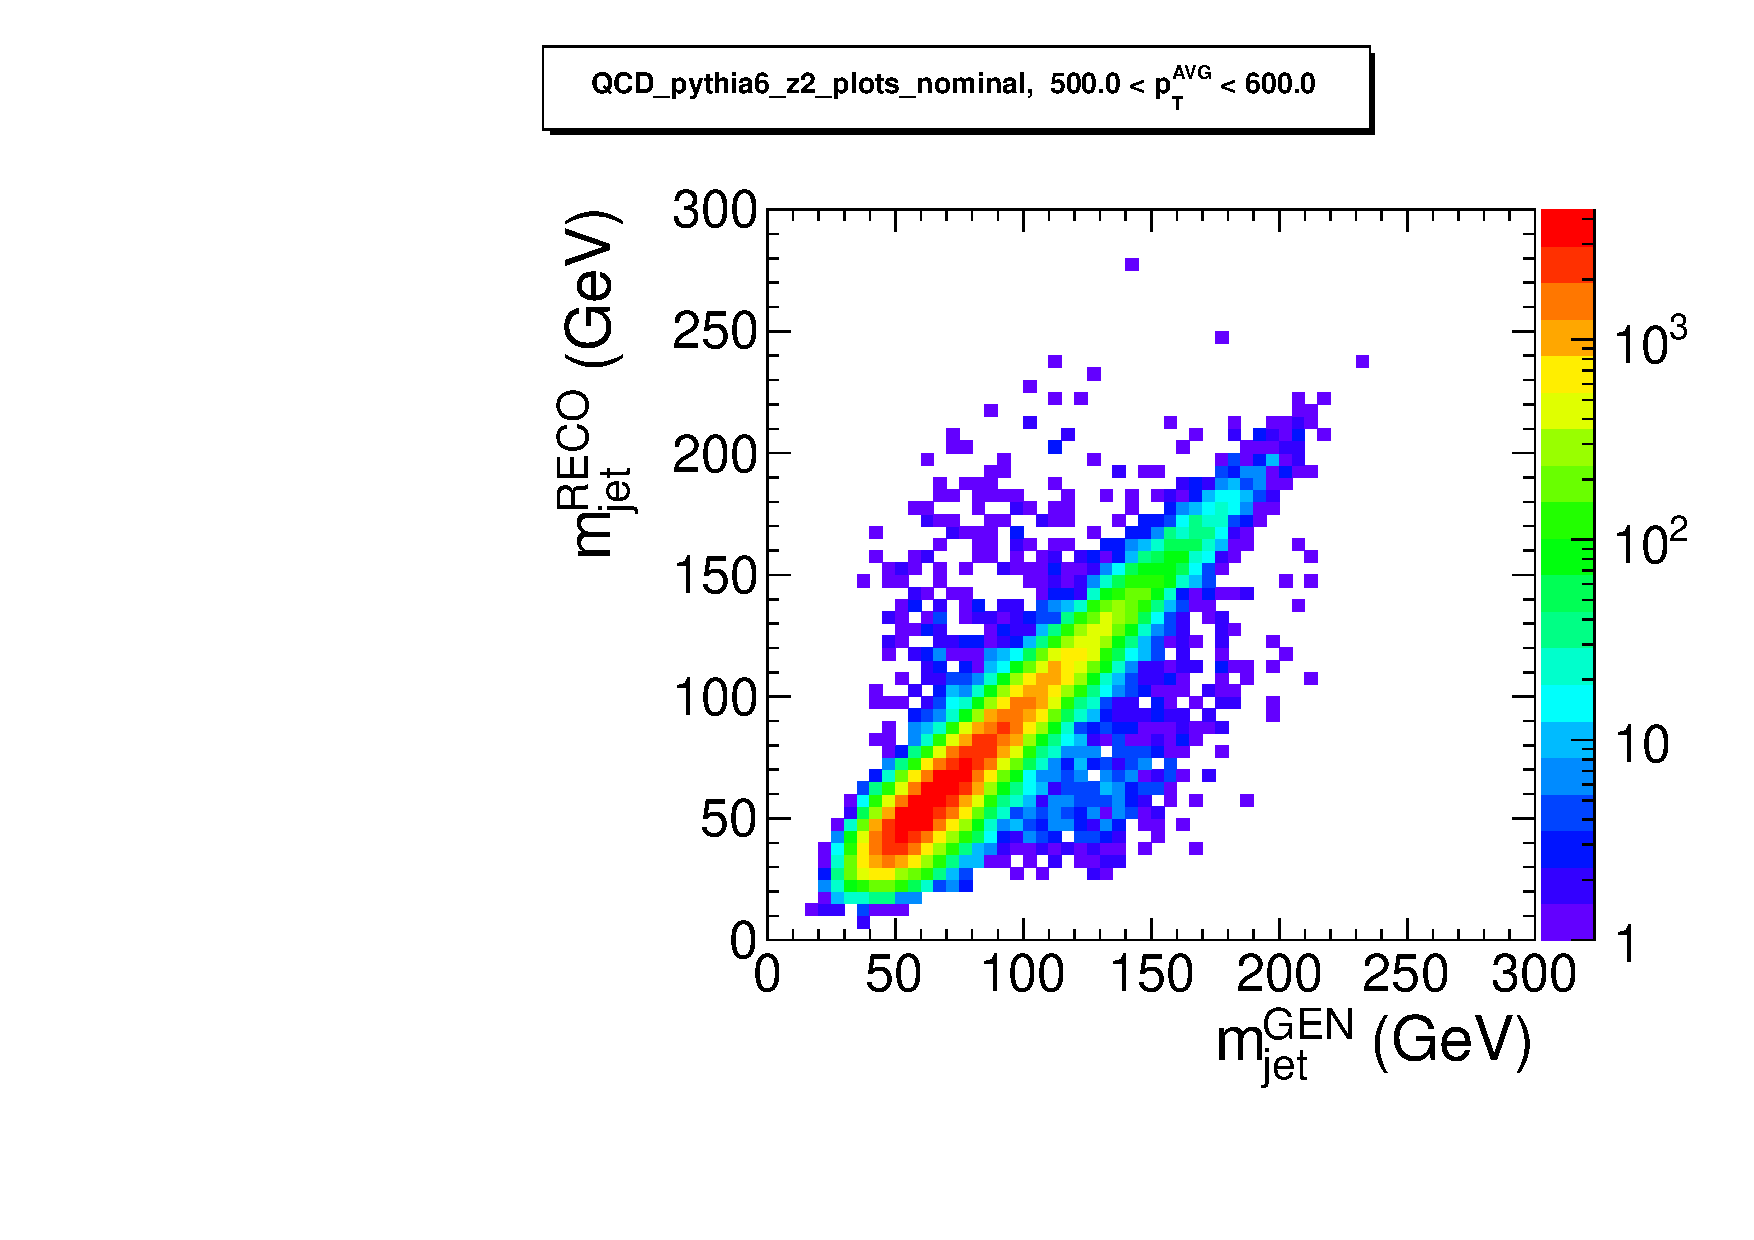
\includegraphics[width=0.3\textwidth]{figs/response_QCD_pythia6_z2_plots_nominal_pt6}}\\
\subfigure{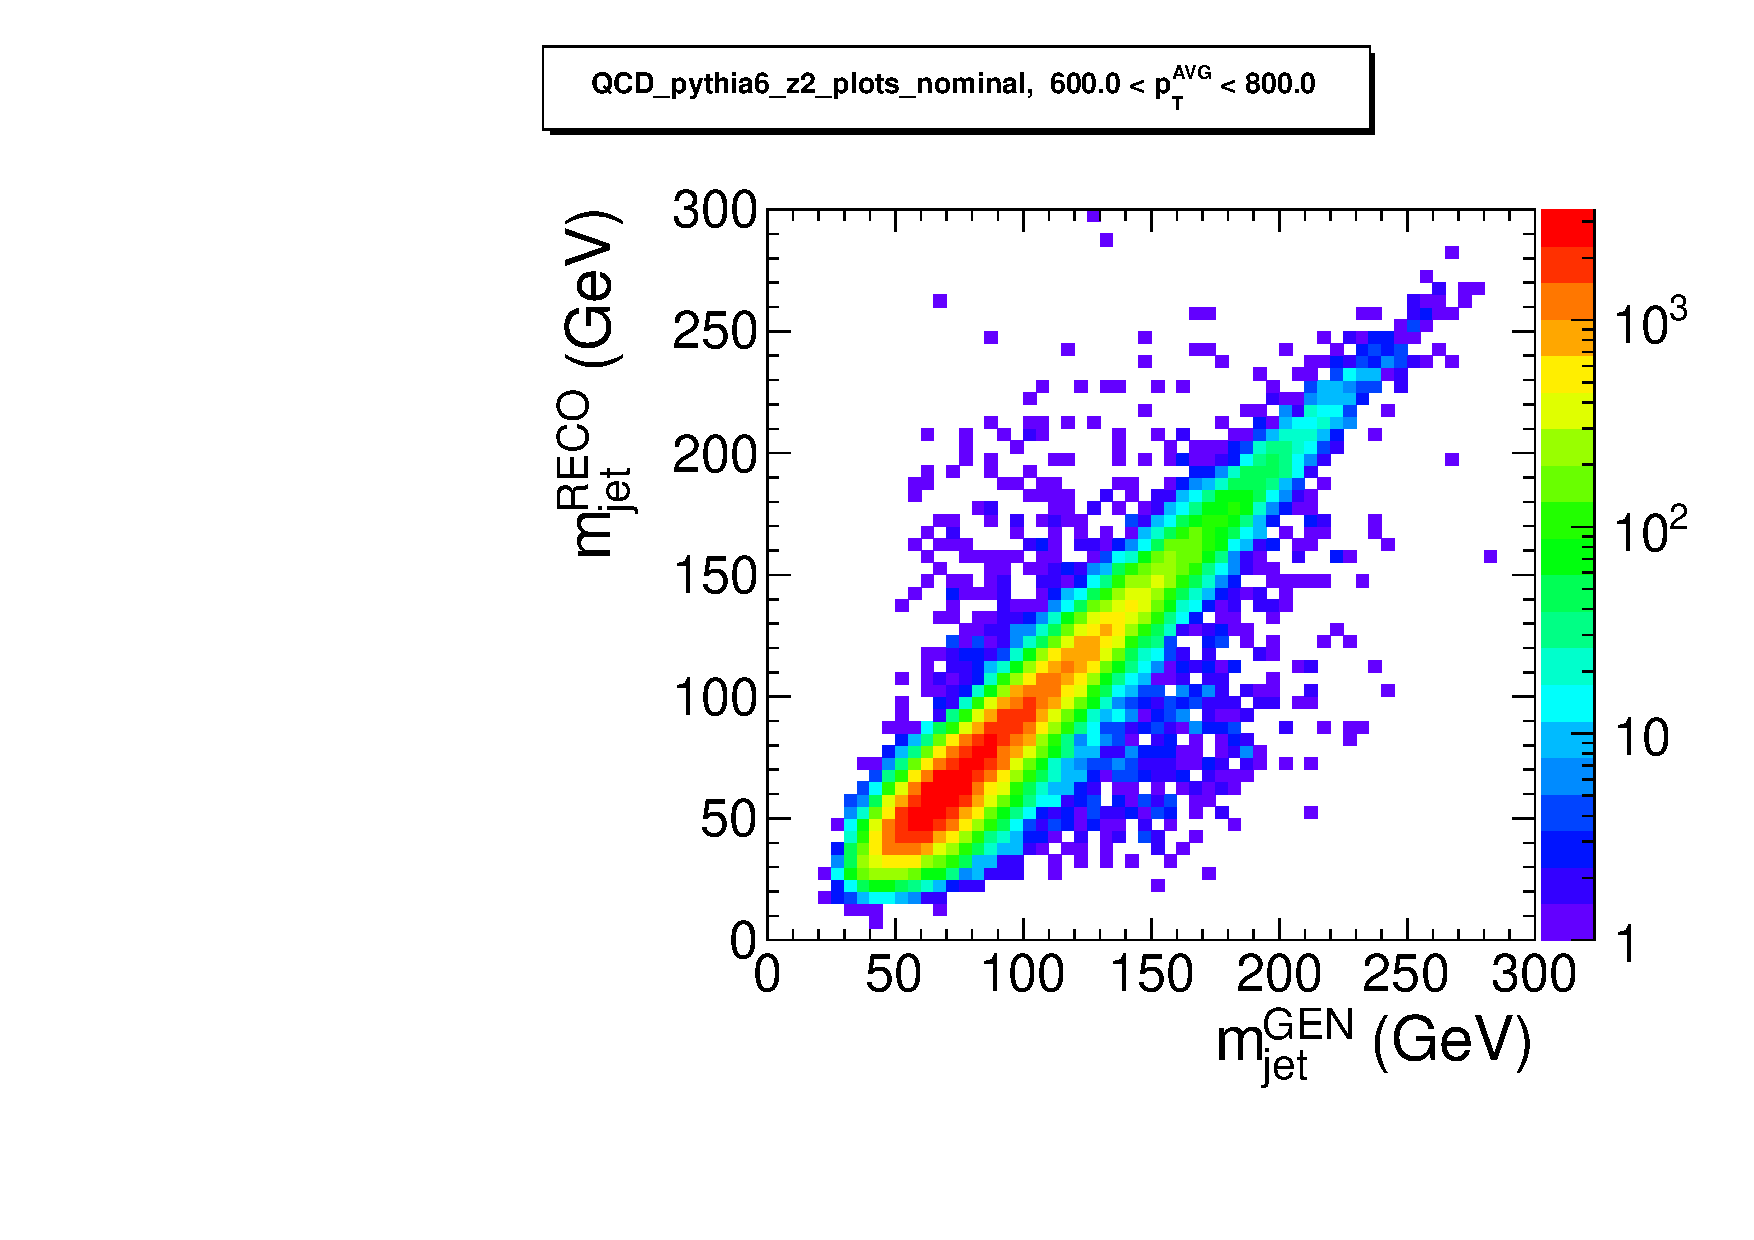
\includegraphics[width=0.3\textwidth]{figs/response_QCD_pythia6_z2_plots_nominal_pt7}}
\subfigure{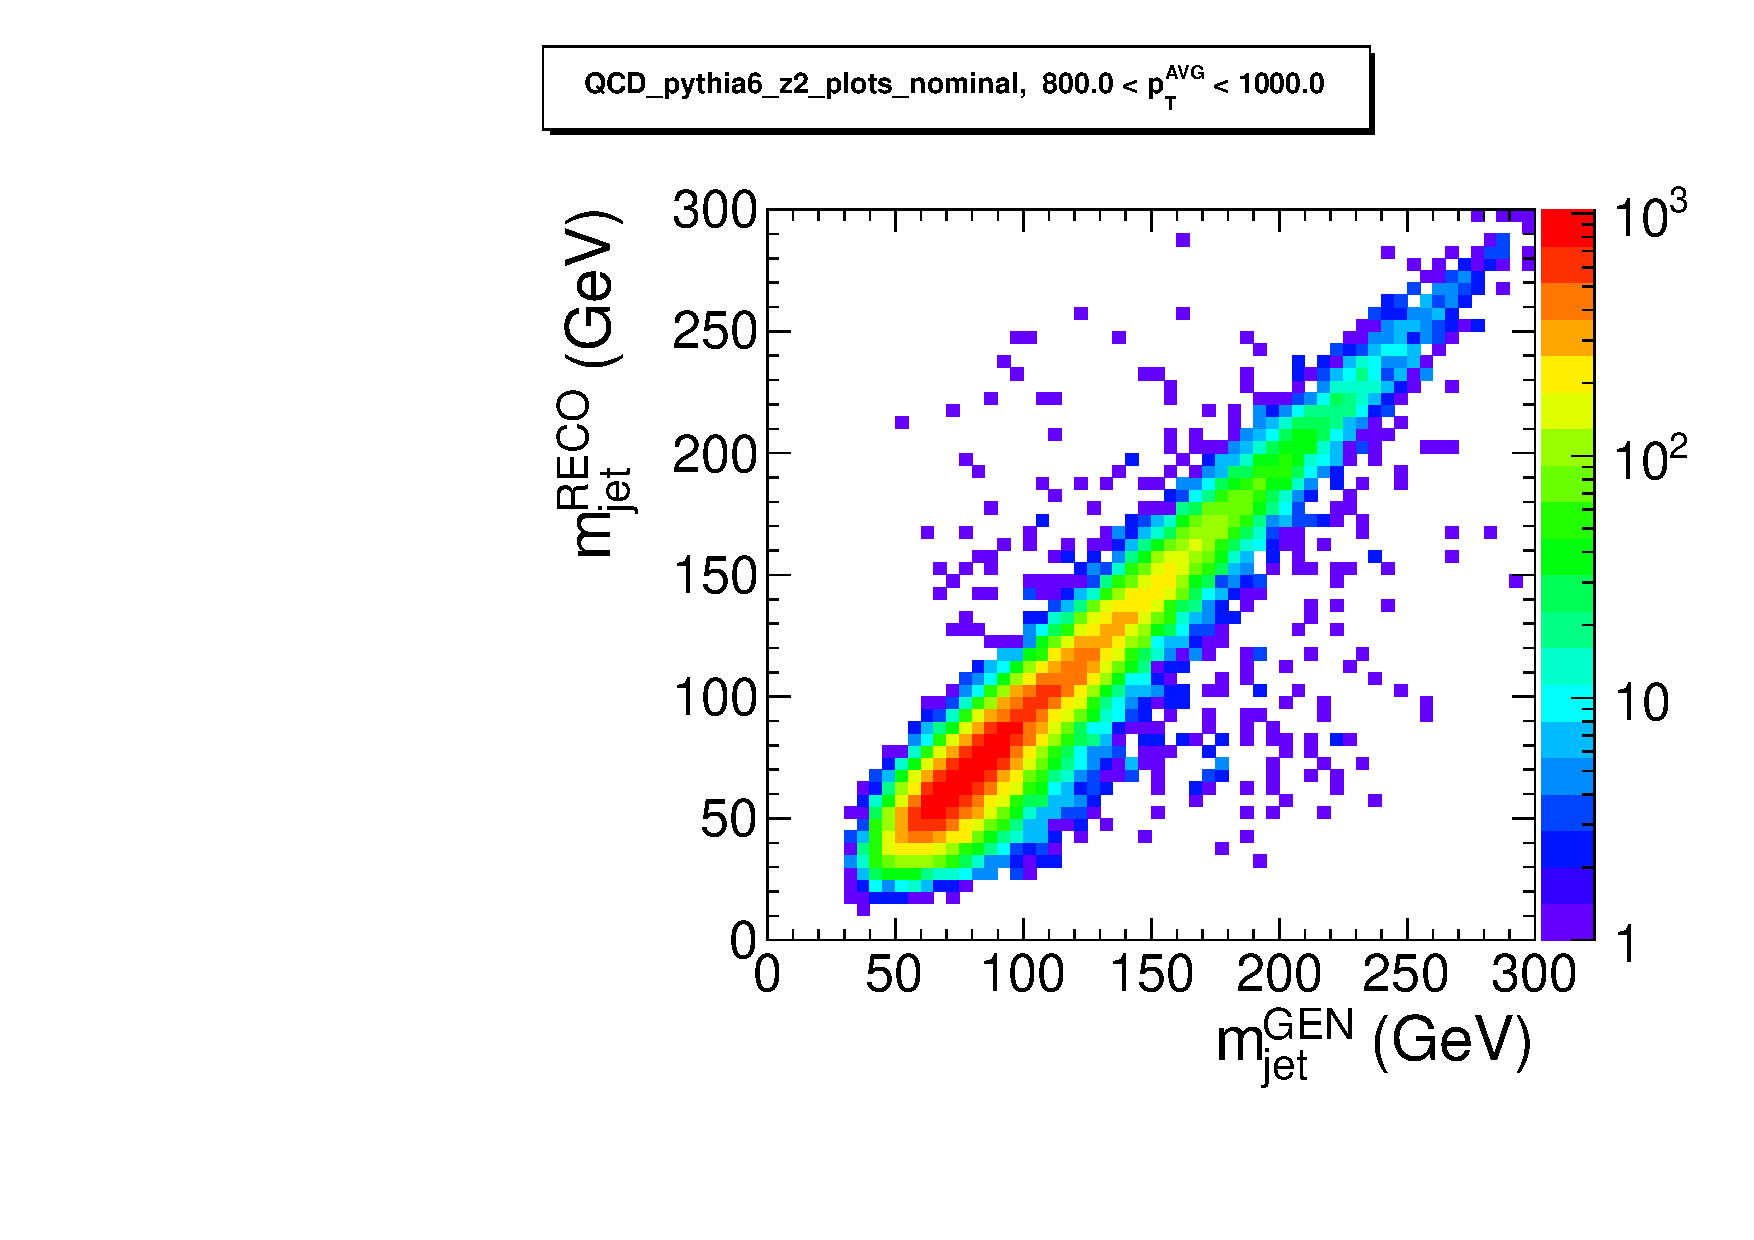
\includegraphics[width=0.3\textwidth]{figs/response_QCD_pythia6_z2_plots_nominal_pt8}}
\subfigure{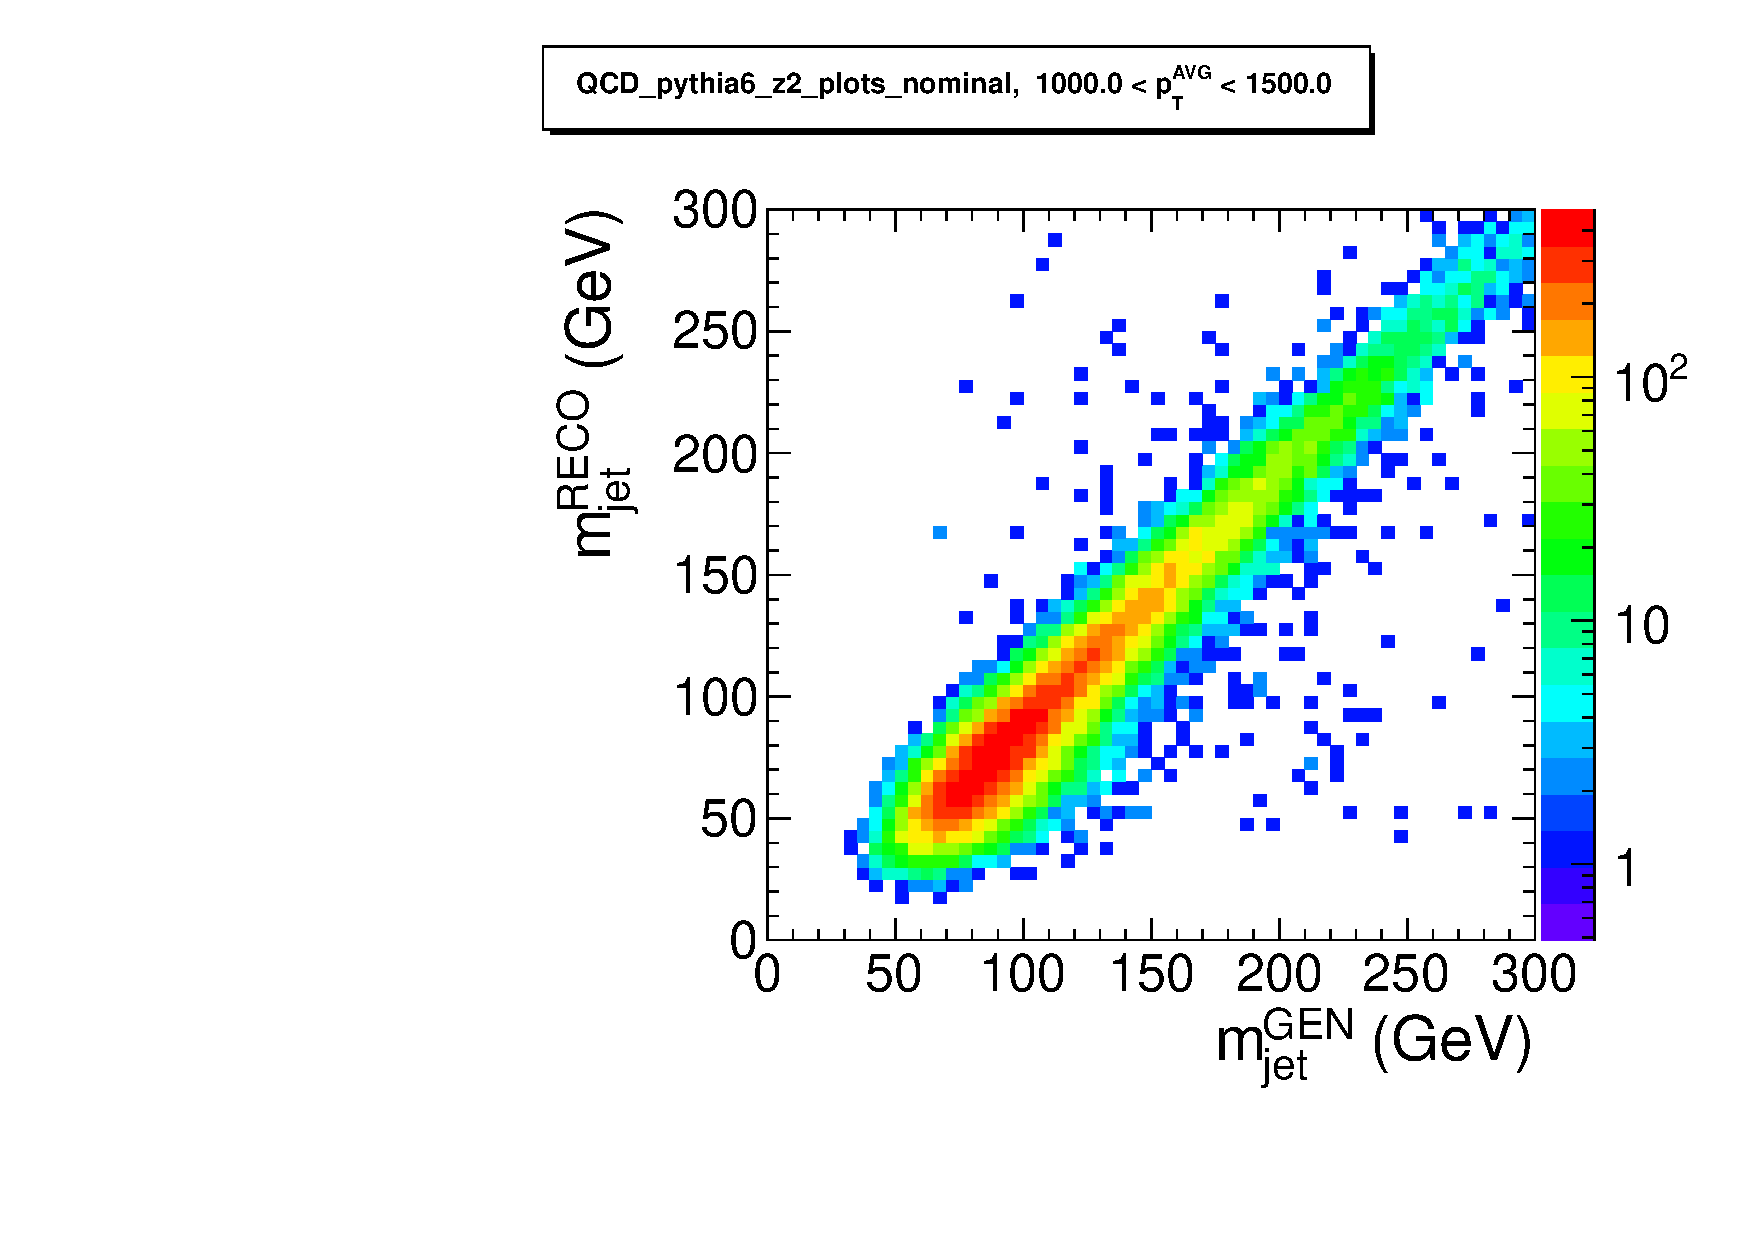
\includegraphics[width=0.3\textwidth]{figs/response_QCD_pythia6_z2_plots_nominal_pt9}}\\
\caption{Response of the jet mass for AK7 jets,
for various $\pt^{AVG}$ bins. The true jet mass is shown
on the $x-$axis, and the reconstructed jet mass is shown on the
$y-$axis, using the \PYTHIA generator. 
\label{figs:response_QCD_pythia6_z2_plots_nominal_ptall}}
\end{figure}


\clearpage

\begin{figure}[htbp]
\centering
\subfigure{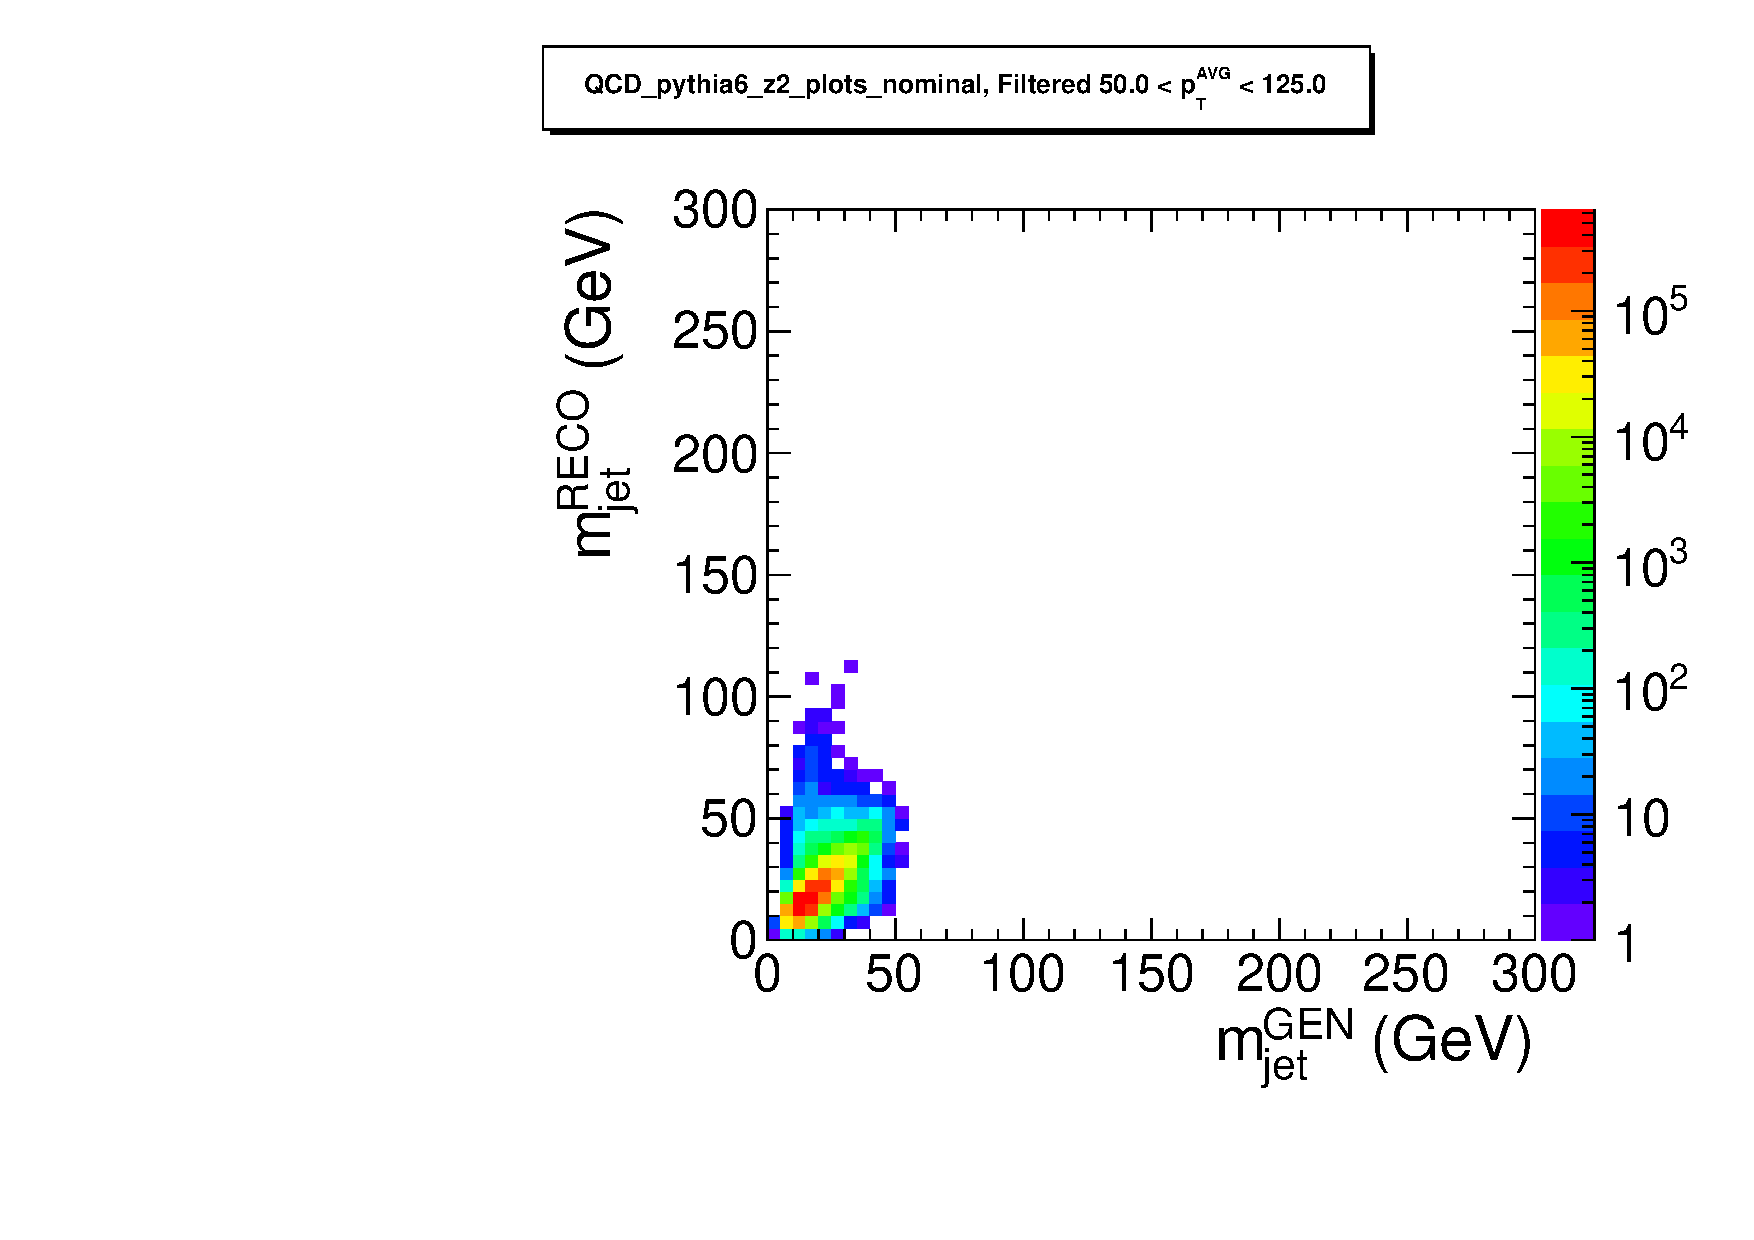
\includegraphics[width=0.3\textwidth]{figs/response_QCD_pythia6_z2_plots_nominal_Filtered_pt1}}
\subfigure{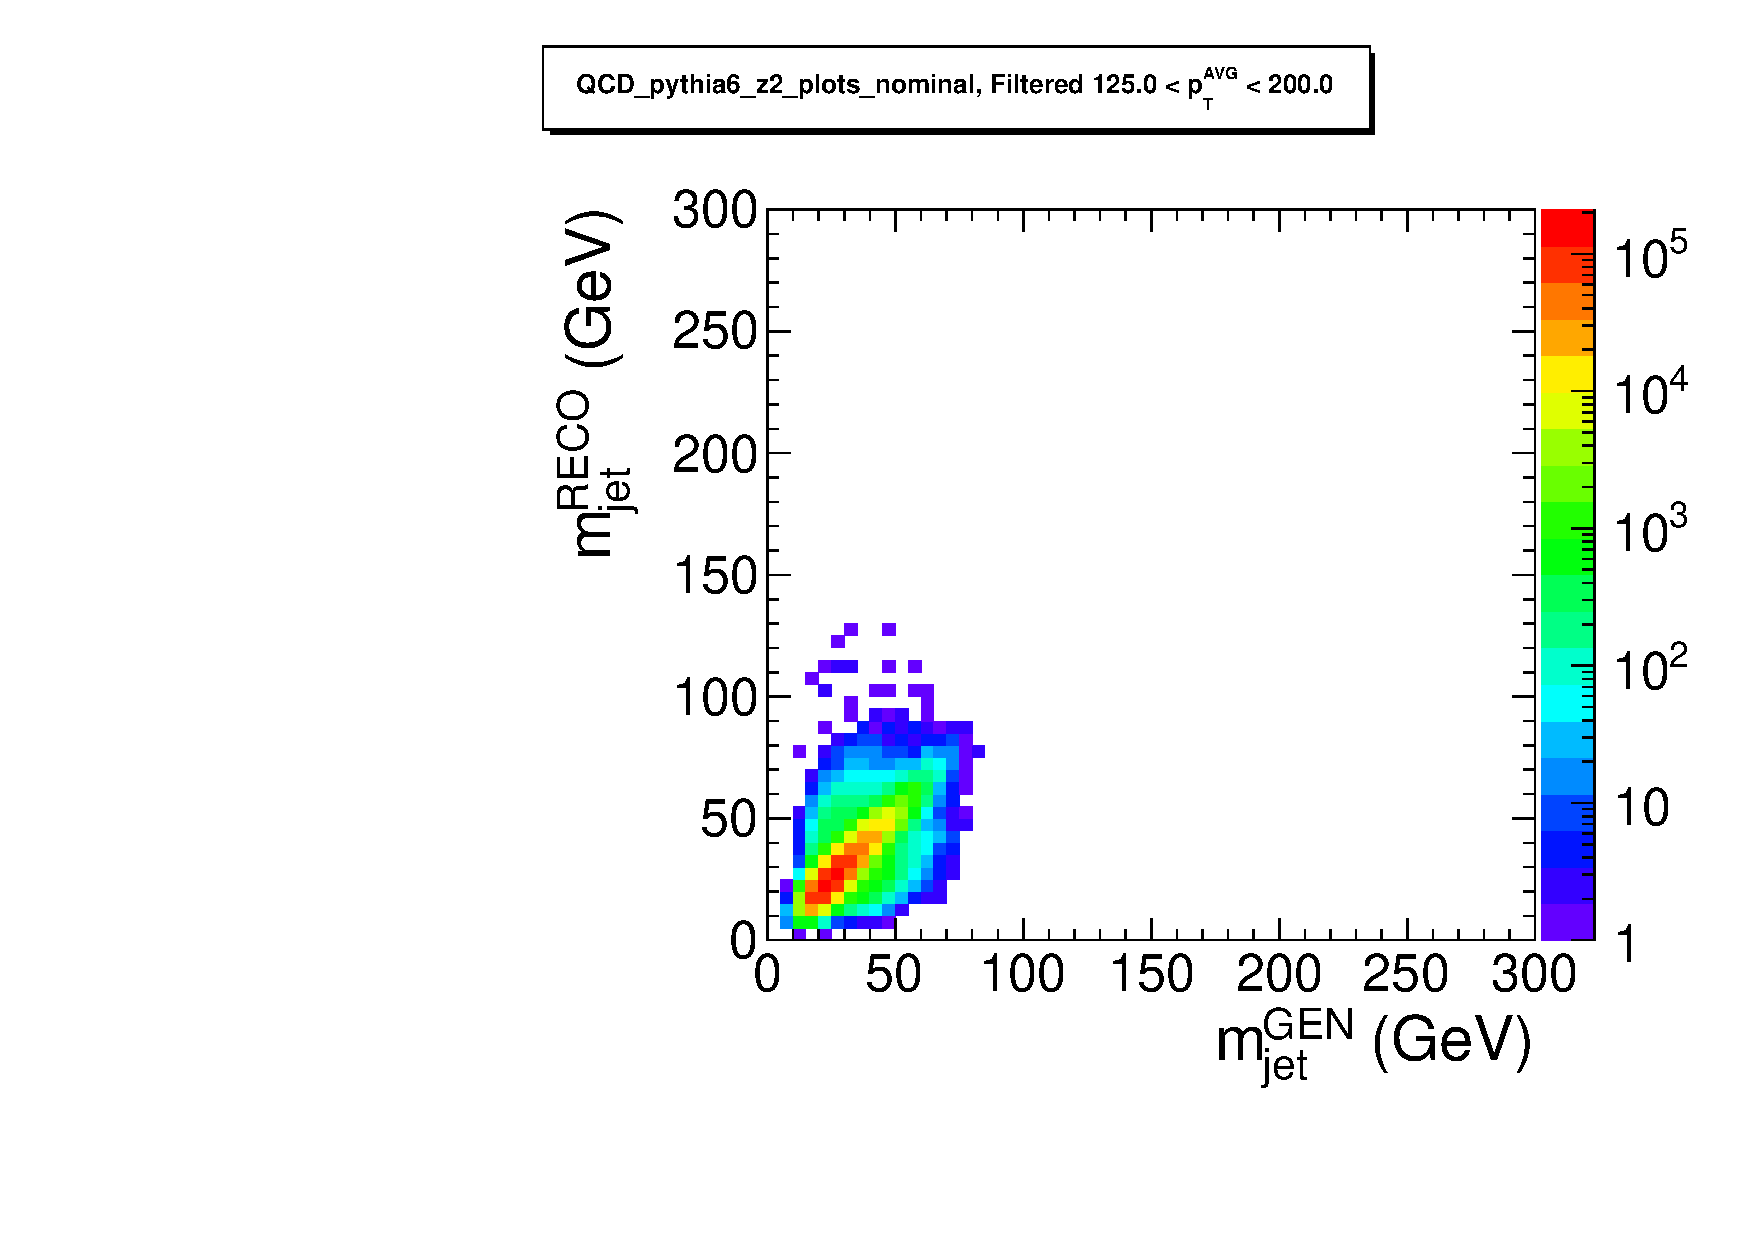
\includegraphics[width=0.3\textwidth]{figs/response_QCD_pythia6_z2_plots_nominal_Filtered_pt2}}
\subfigure{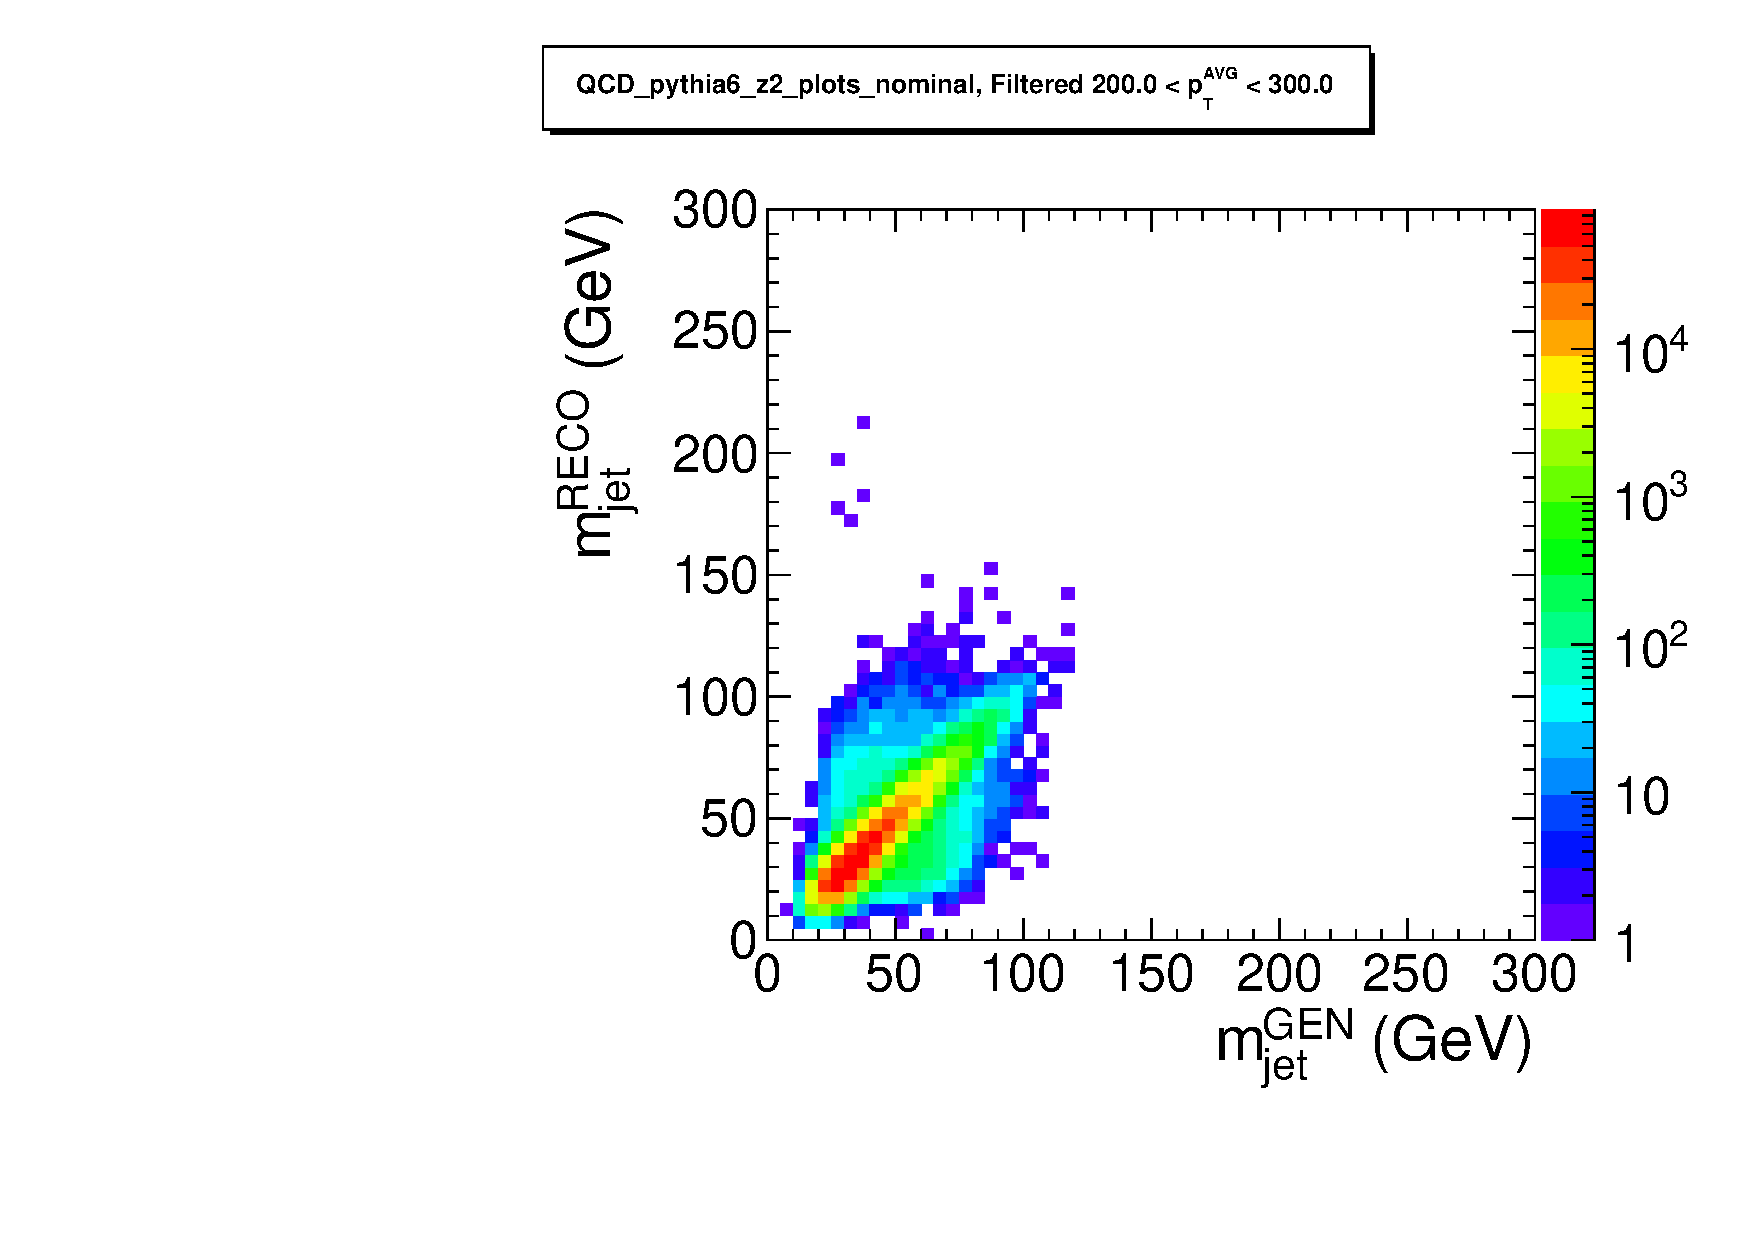
\includegraphics[width=0.3\textwidth]{figs/response_QCD_pythia6_z2_plots_nominal_Filtered_pt3}}\\
\subfigure{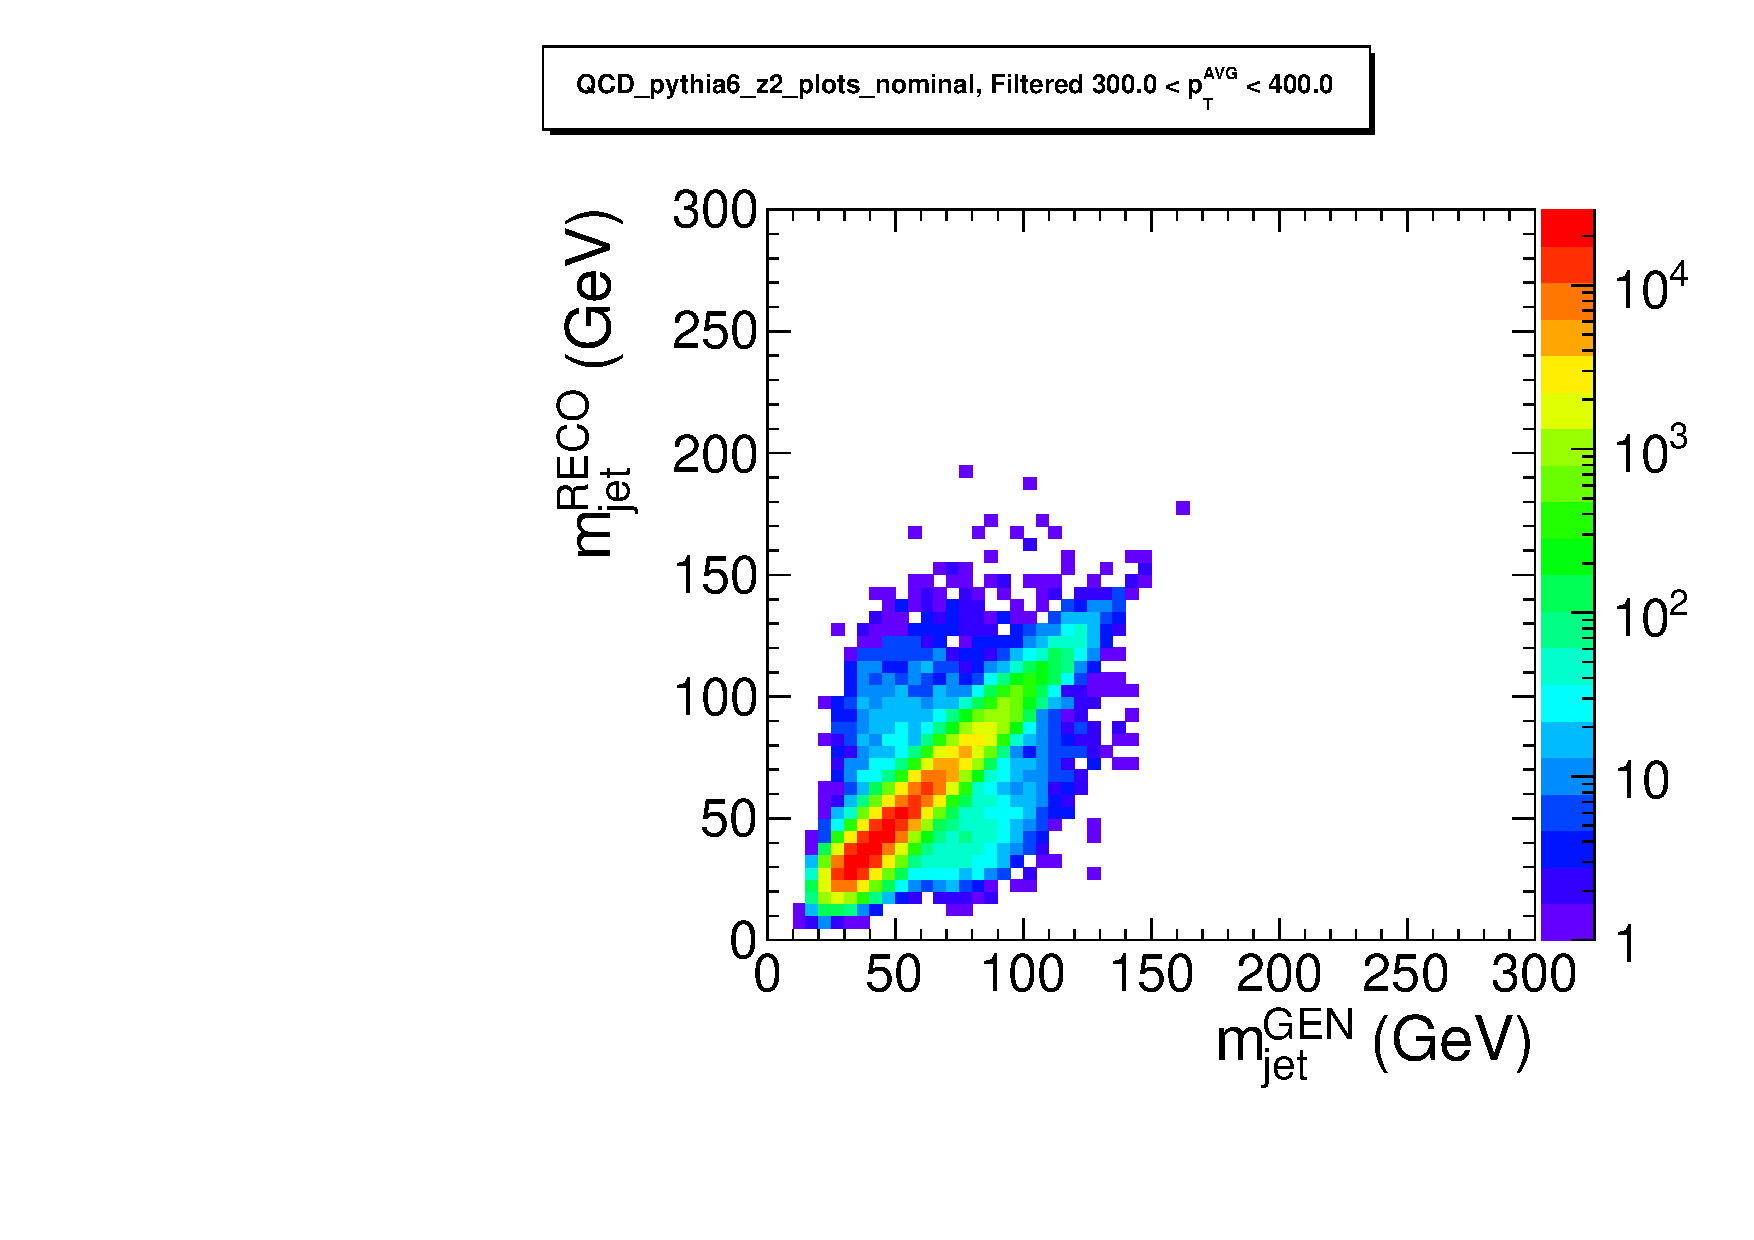
\includegraphics[width=0.3\textwidth]{figs/response_QCD_pythia6_z2_plots_nominal_Filtered_pt4}}
\subfigure{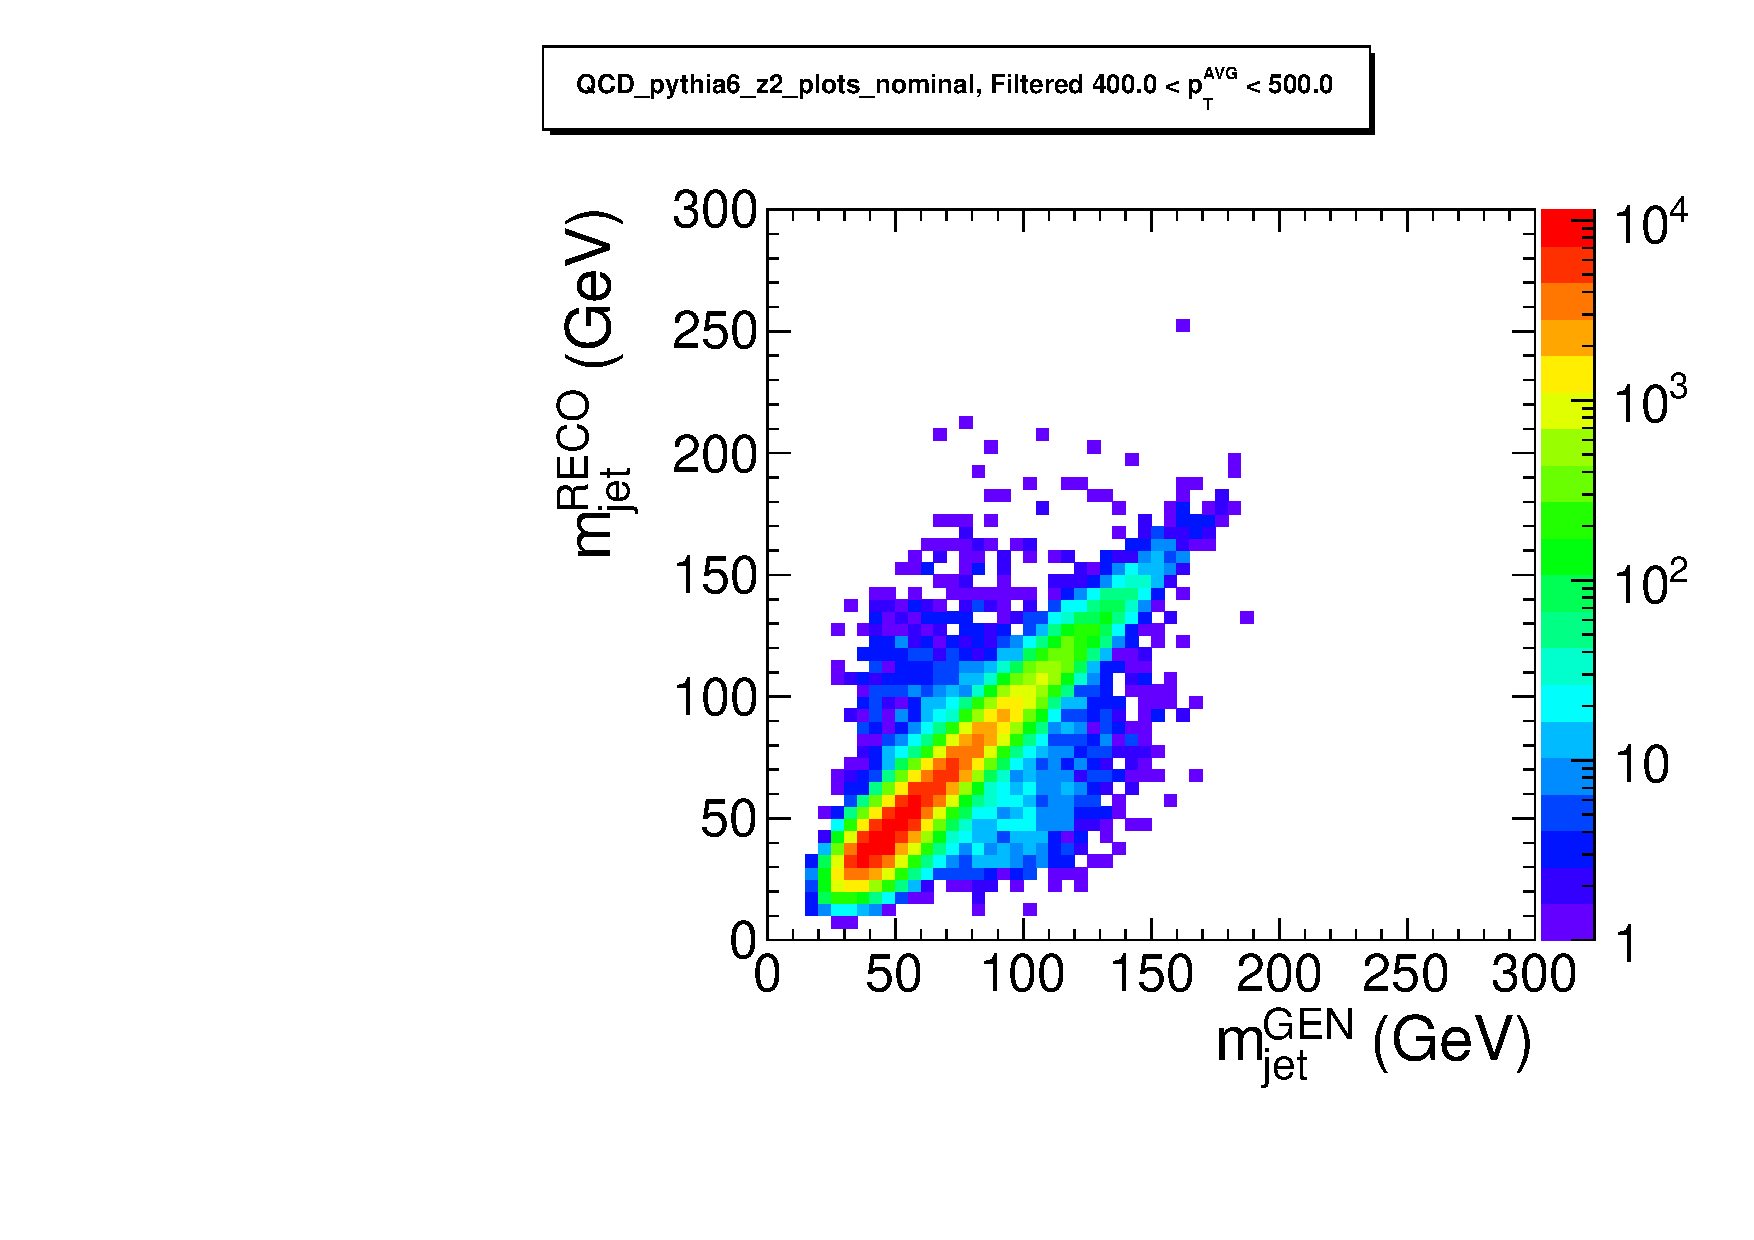
\includegraphics[width=0.3\textwidth]{figs/response_QCD_pythia6_z2_plots_nominal_Filtered_pt5}}
\subfigure{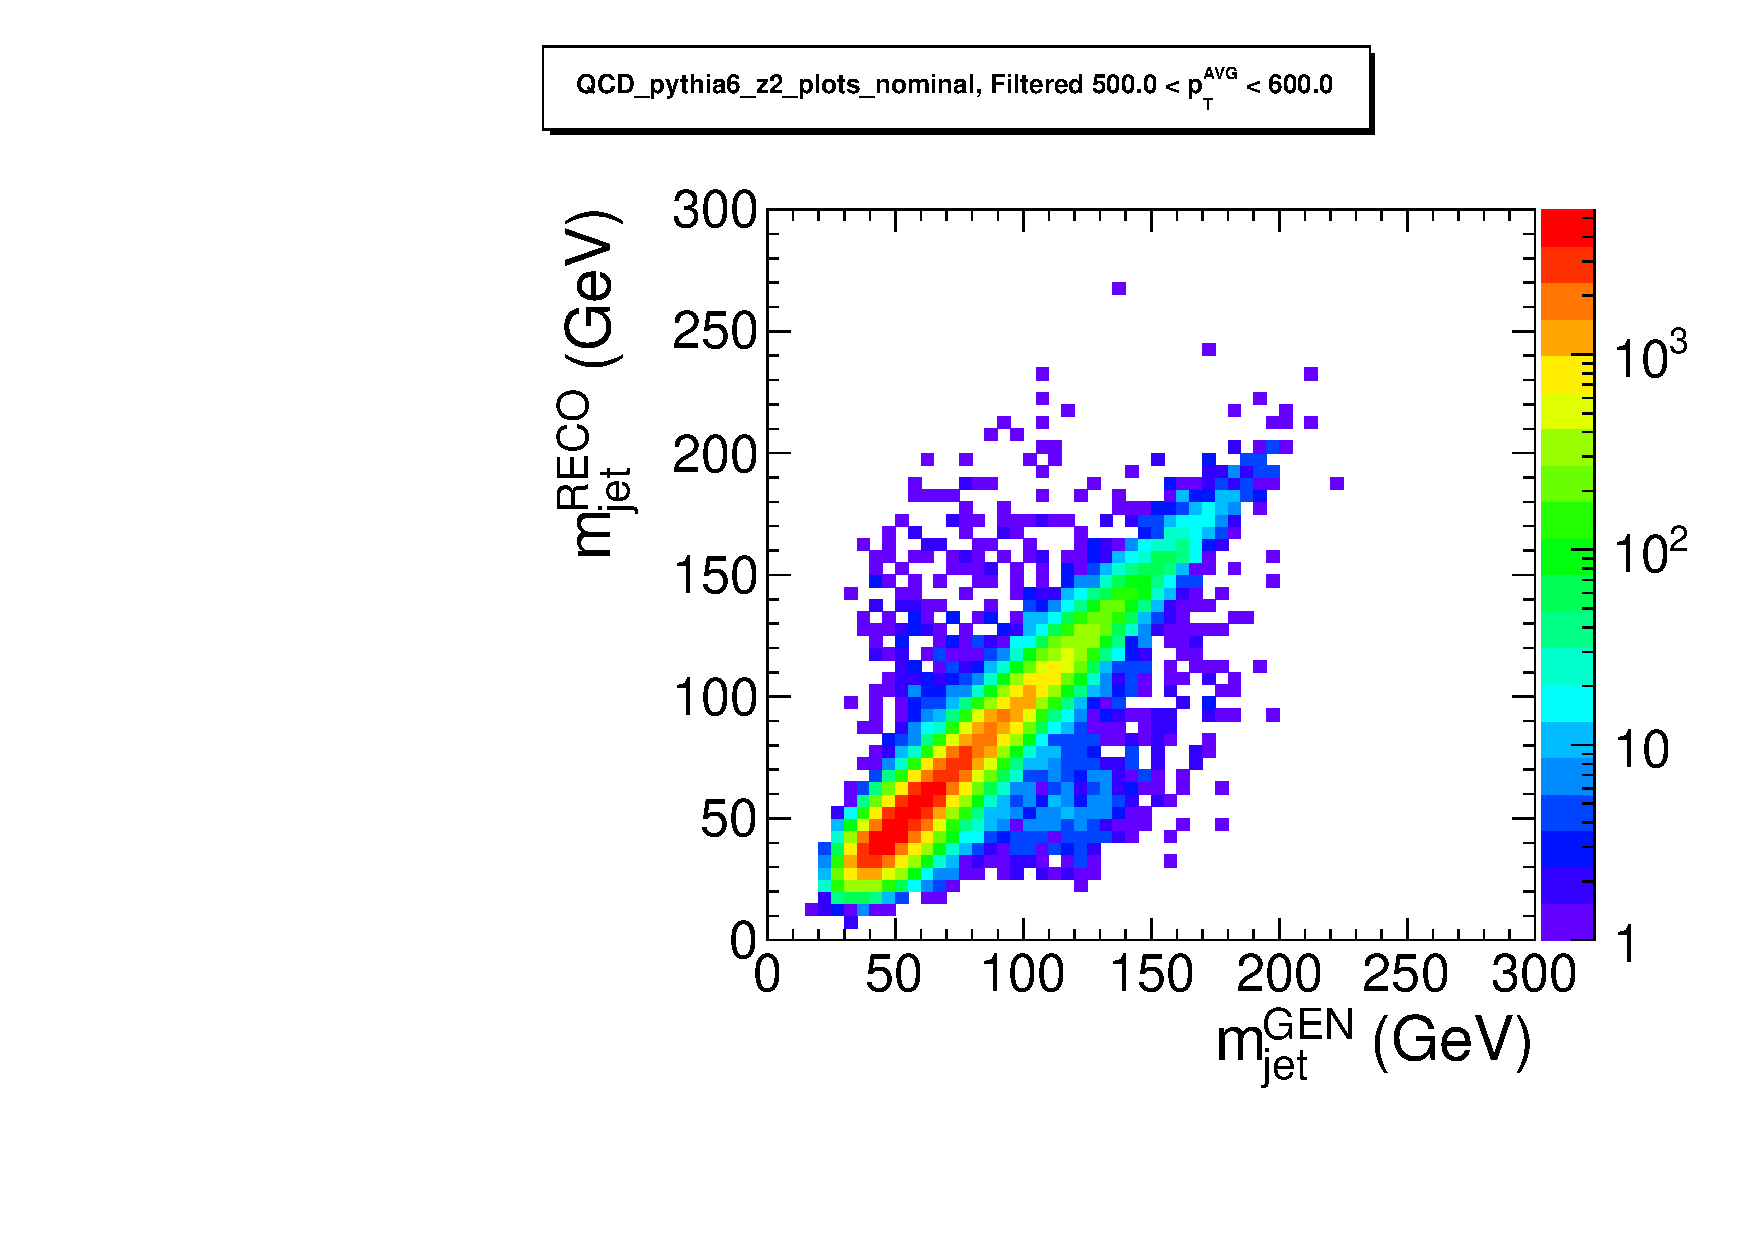
\includegraphics[width=0.3\textwidth]{figs/response_QCD_pythia6_z2_plots_nominal_Filtered_pt6}}\\
\subfigure{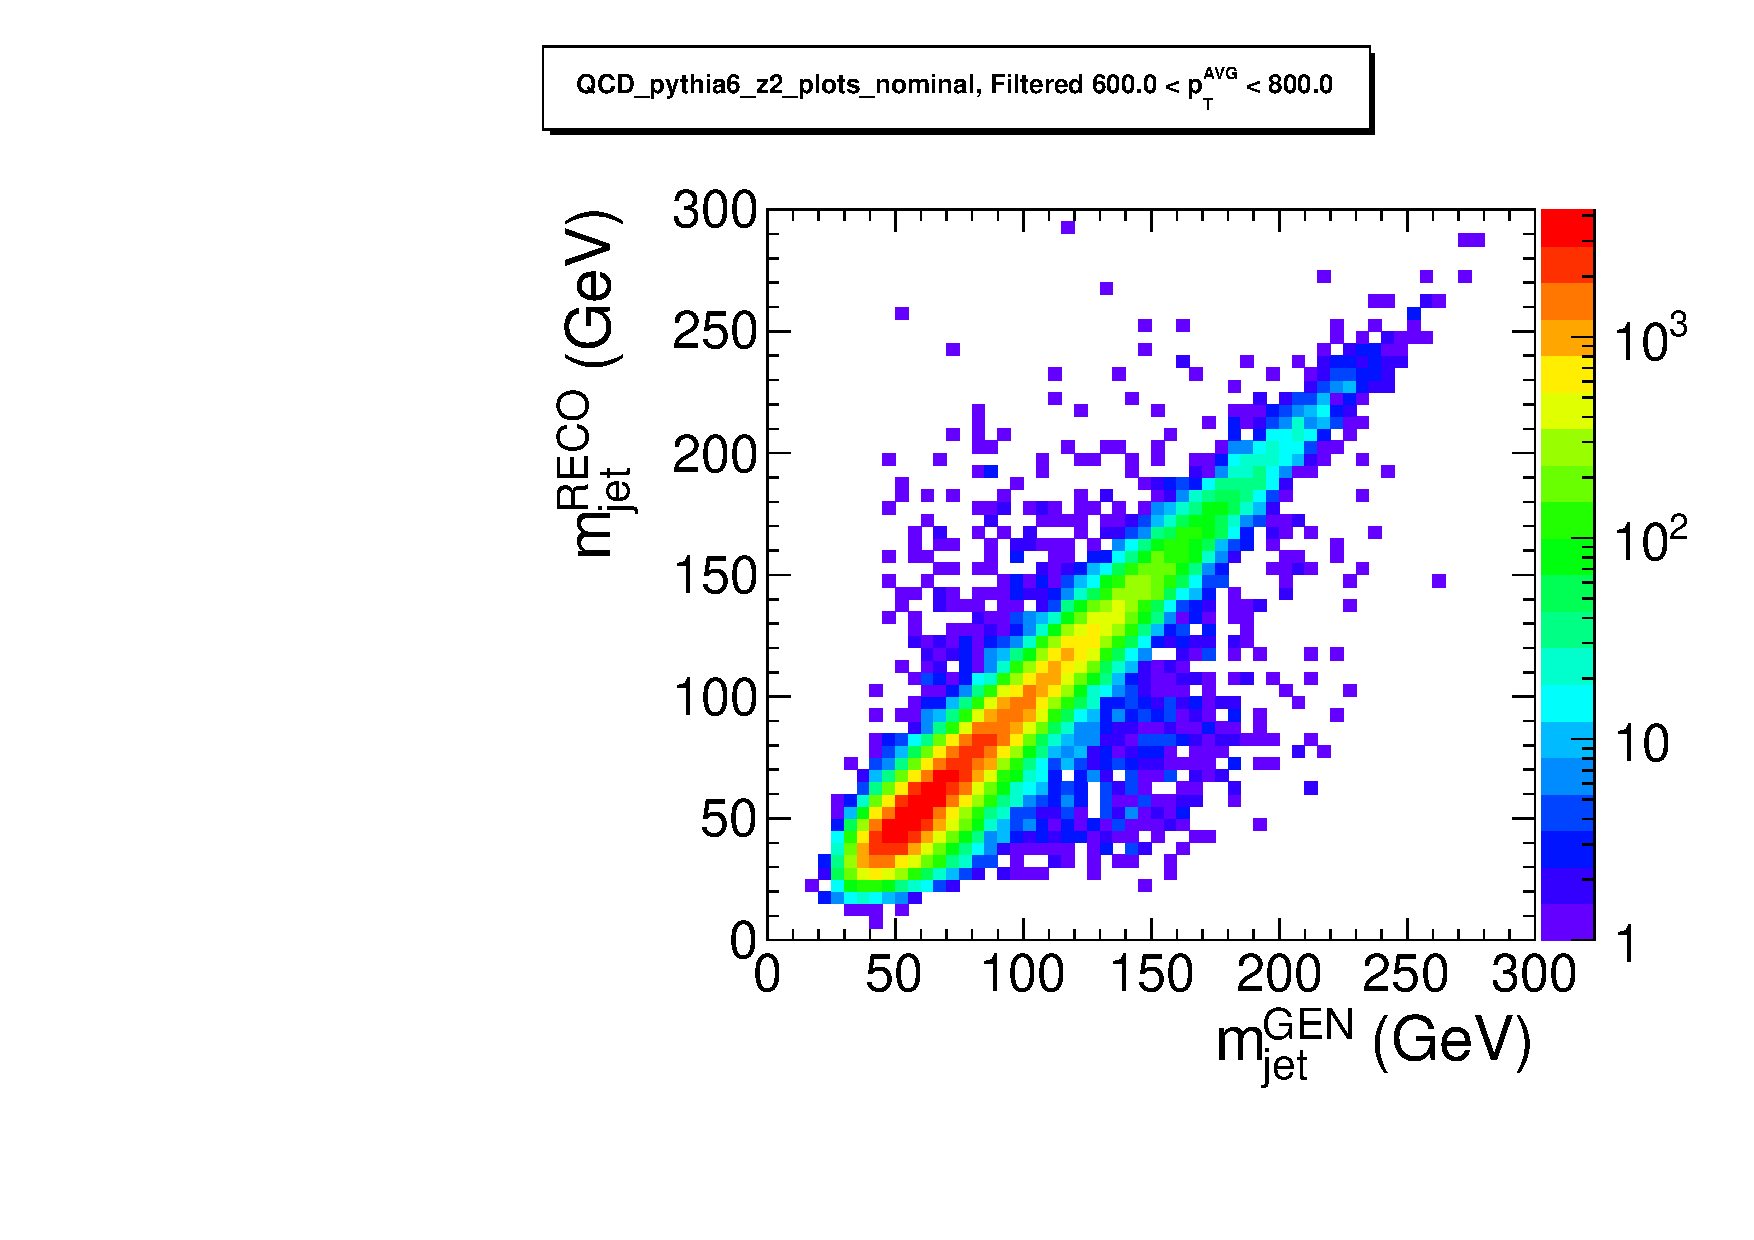
\includegraphics[width=0.3\textwidth]{figs/response_QCD_pythia6_z2_plots_nominal_Filtered_pt7}}
\subfigure{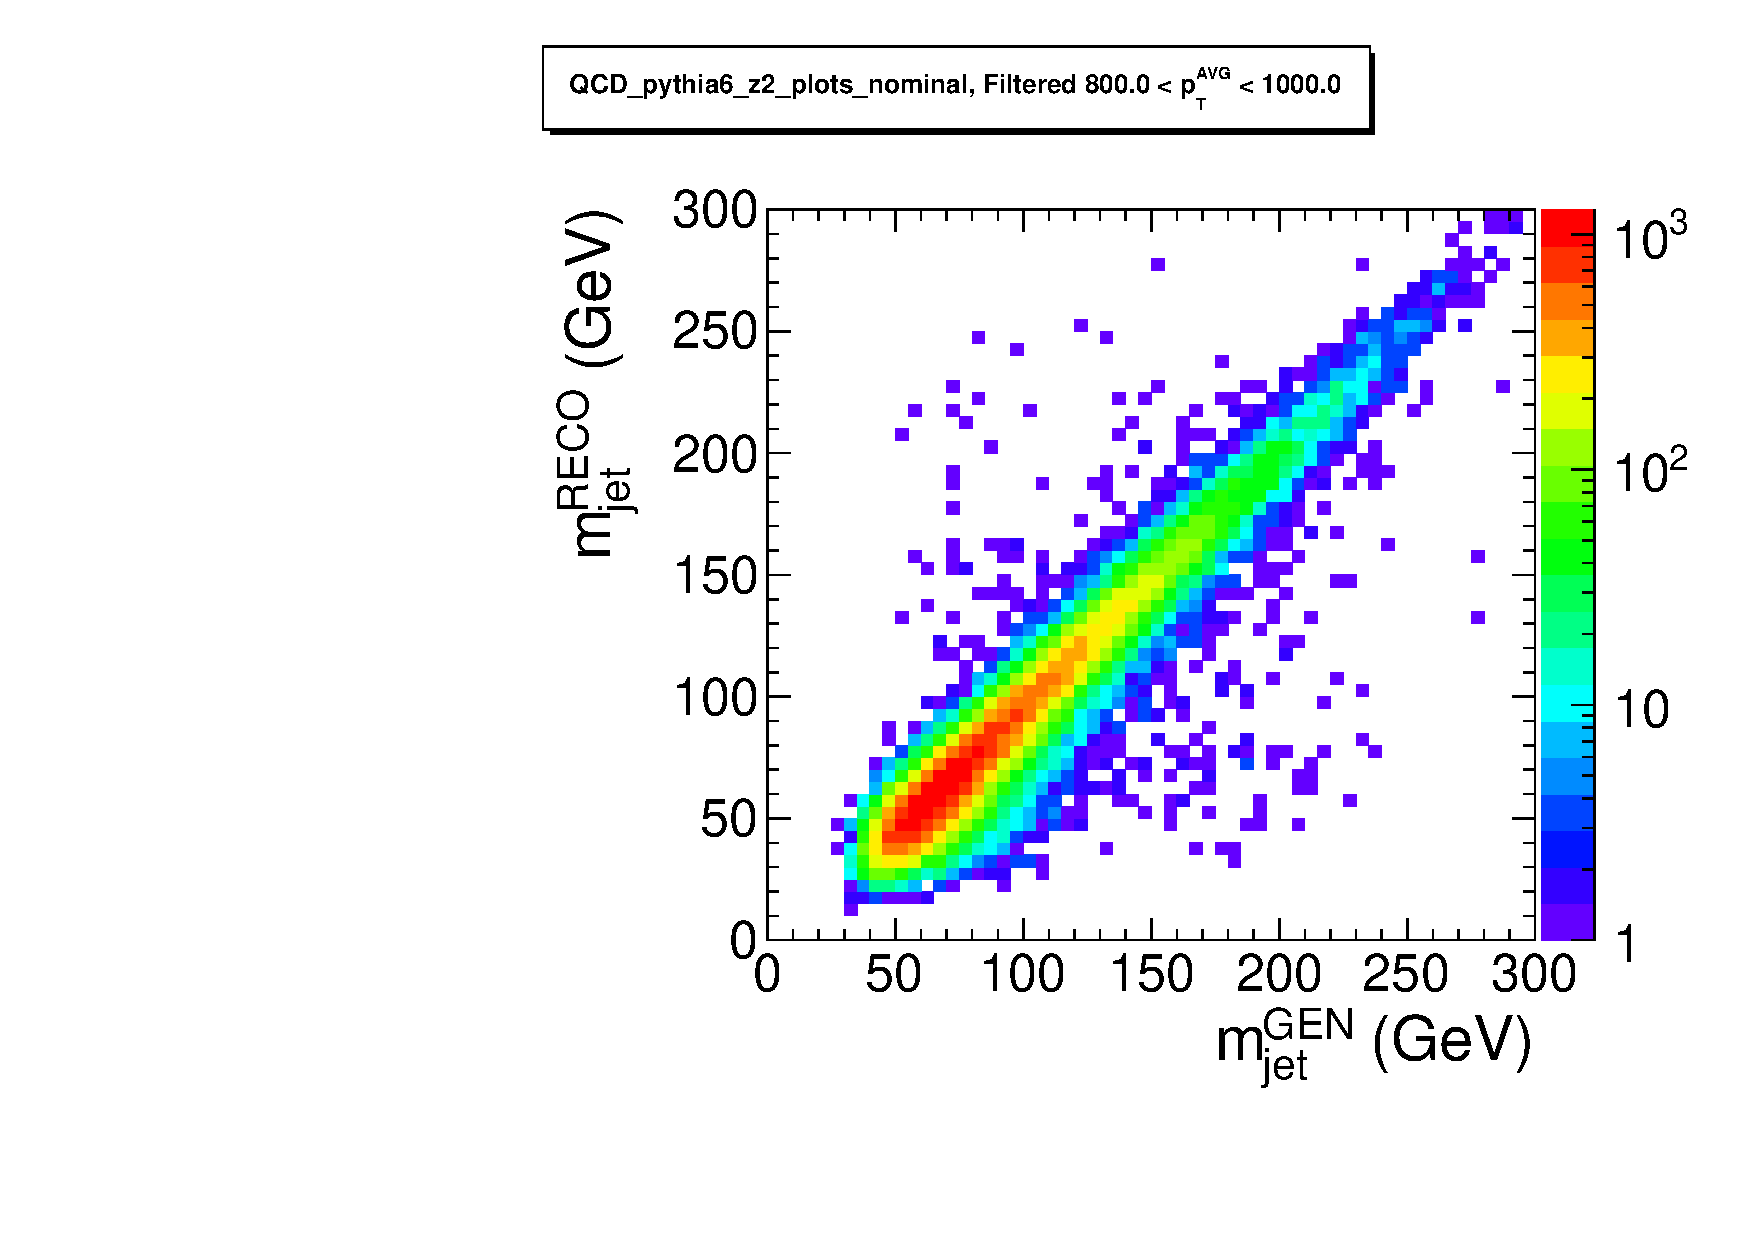
\includegraphics[width=0.3\textwidth]{figs/response_QCD_pythia6_z2_plots_nominal_Filtered_pt8}}
\subfigure{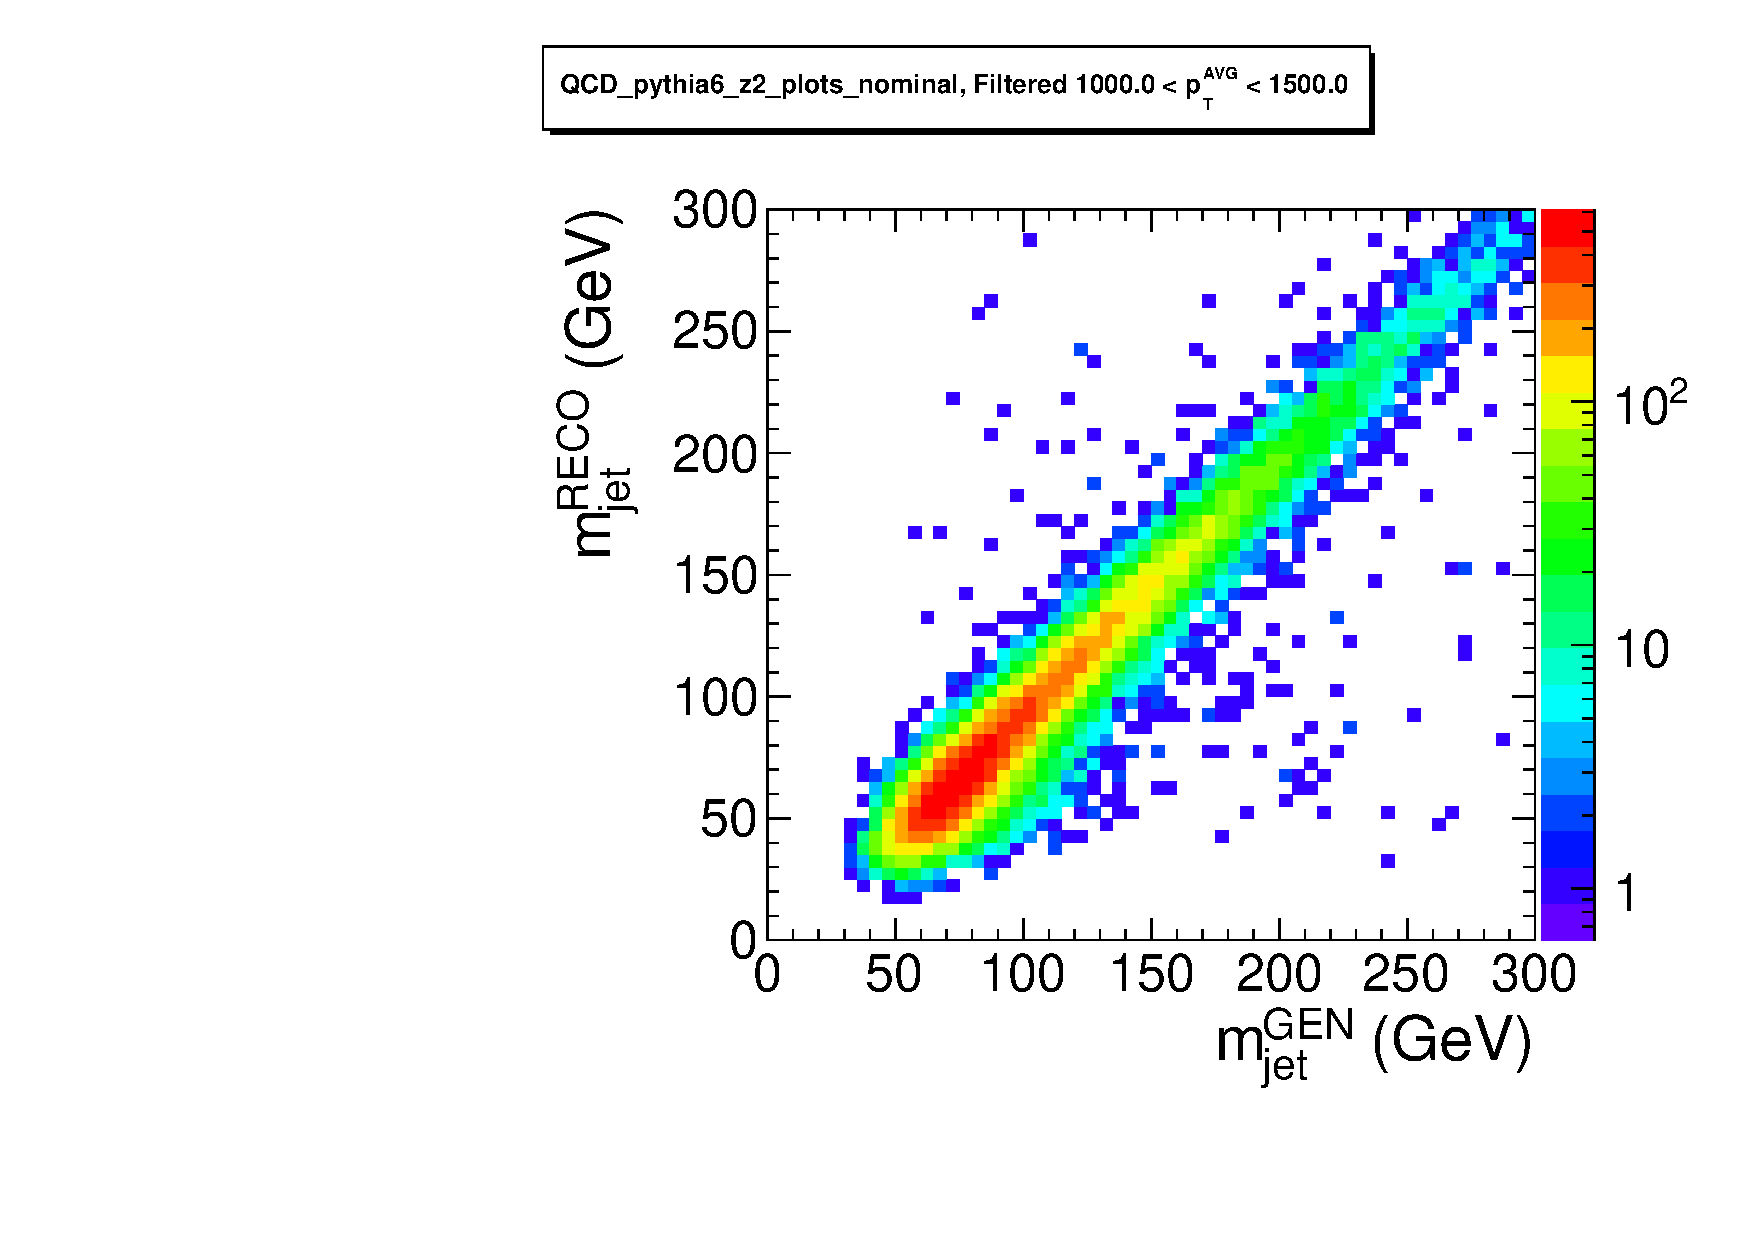
\includegraphics[width=0.3\textwidth]{figs/response_QCD_pythia6_z2_plots_nominal_Filtered_pt9}}\\
\caption{Response of the jet mass for AK7 Filteredjets,
for various $\pt^{AVG}$ bins. The true jet mass is shown
on the $x-$axis, and the reconstructed jet mass is shown on the
$y-$axis, using the \PYTHIA generator. 
\label{figs:response_QCD_pythia6_z2_plots_nominal_Filtered_ptall}}
\end{figure}


\clearpage

\begin{figure}[htbp]
\centering
\subfigure{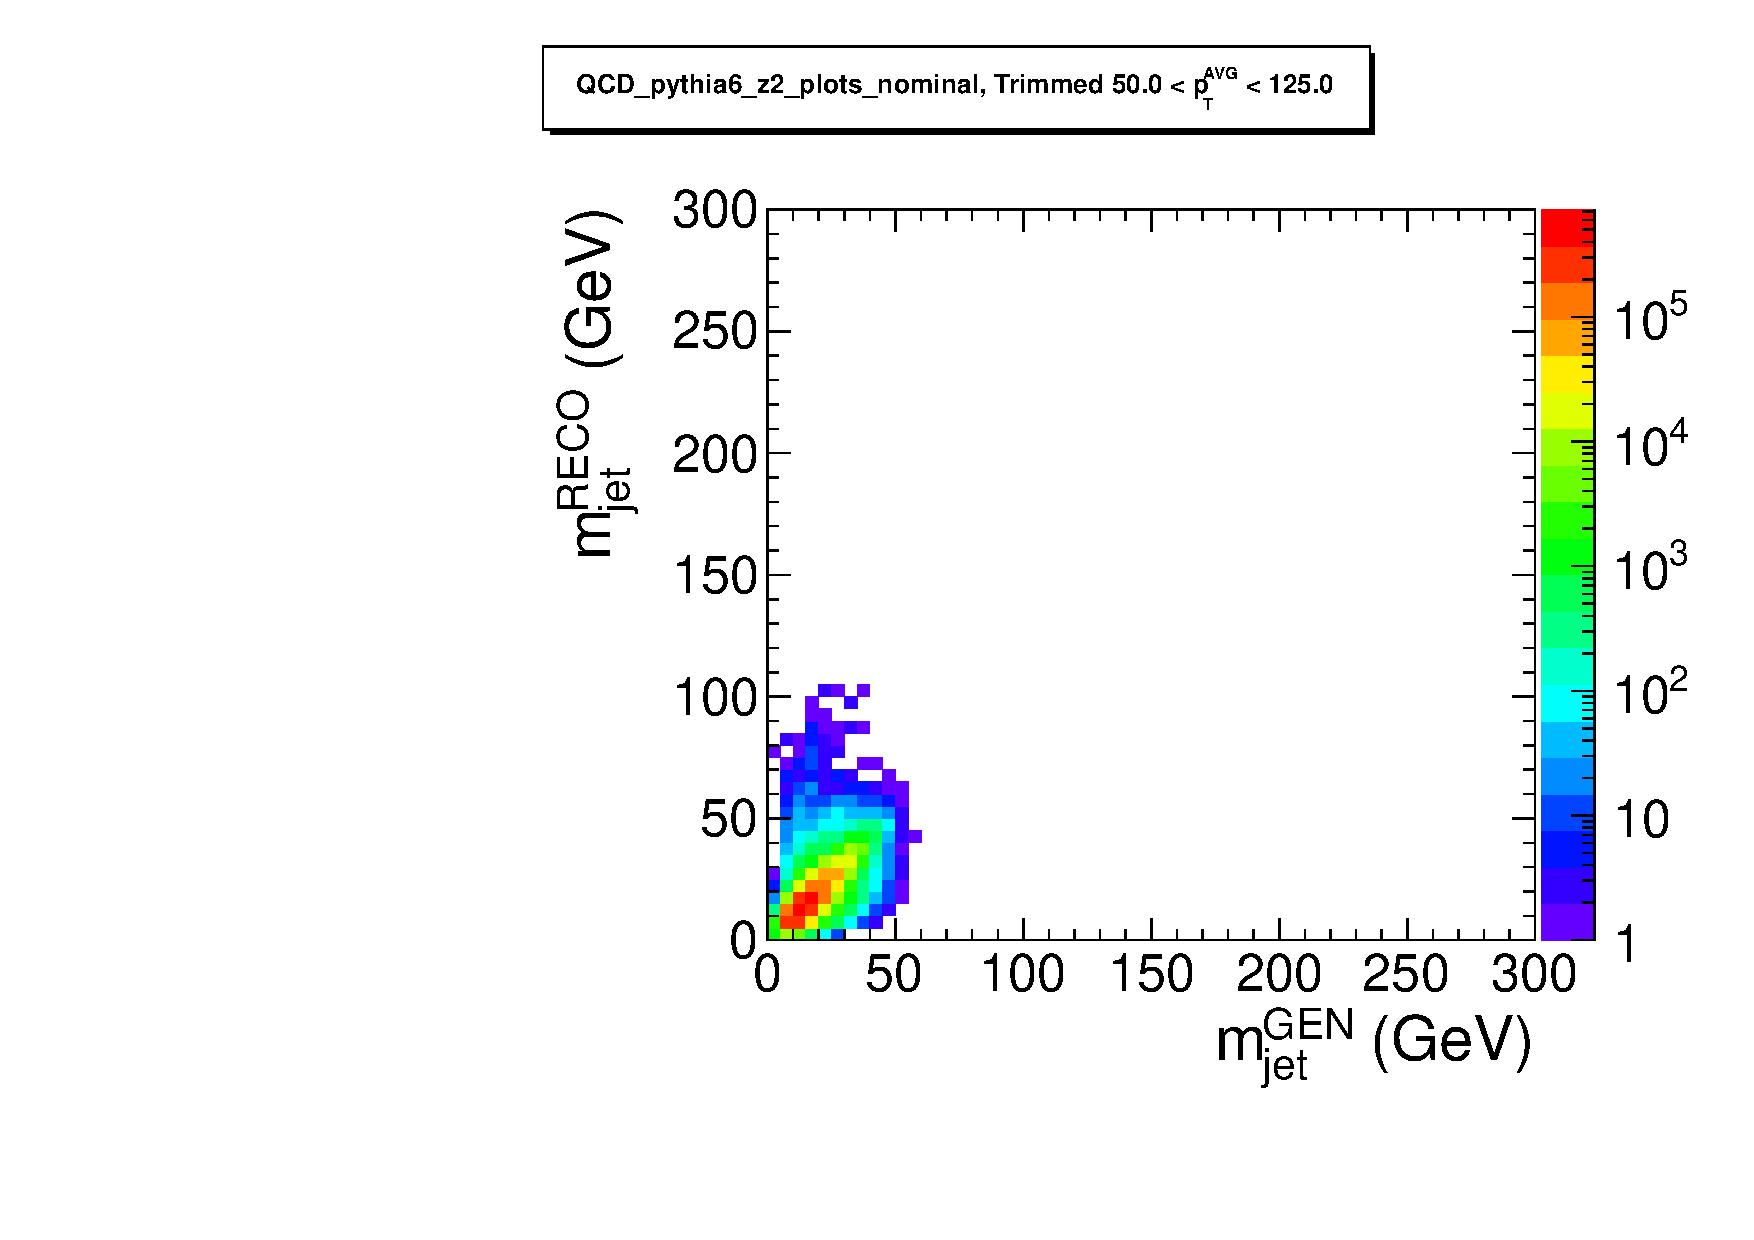
\includegraphics[width=0.3\textwidth]{figs/response_QCD_pythia6_z2_plots_nominal_Trimmed_pt1}}
\subfigure{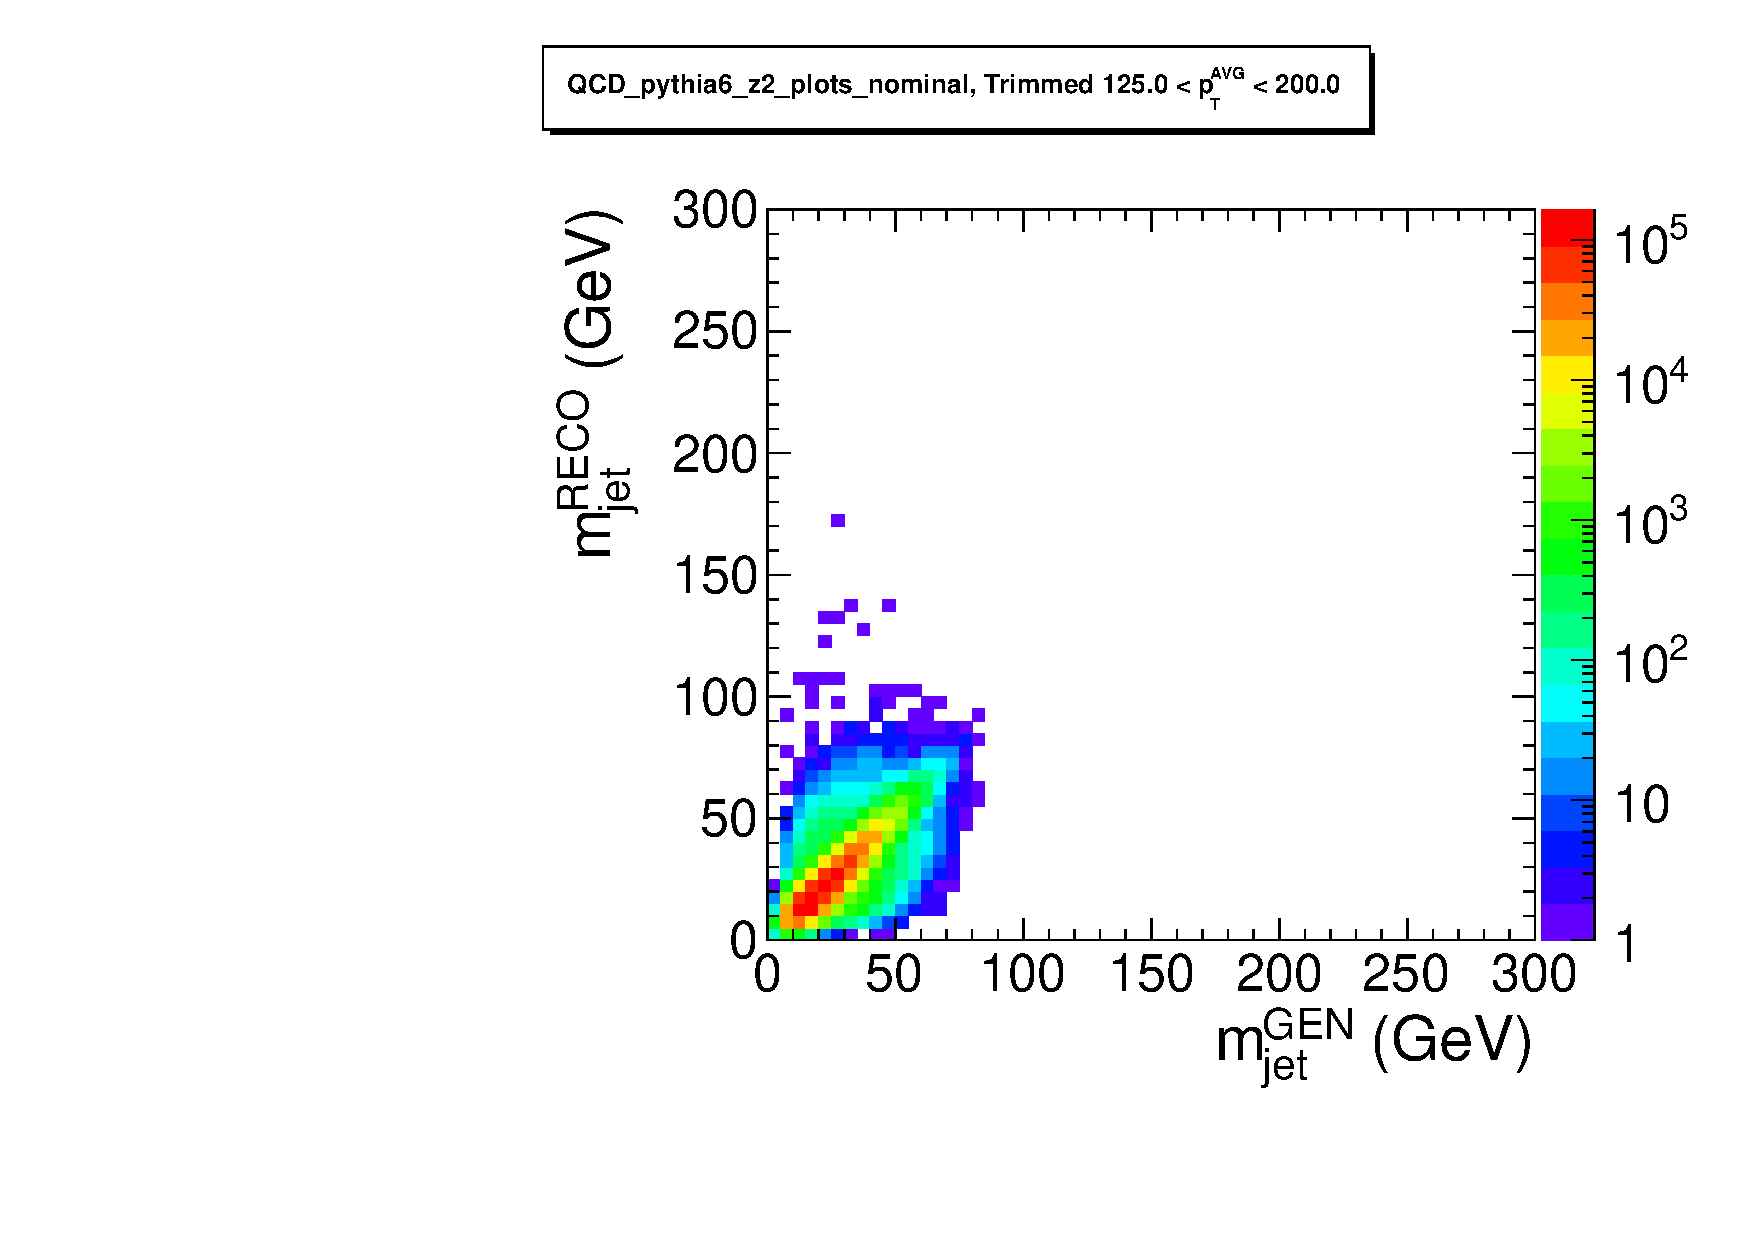
\includegraphics[width=0.3\textwidth]{figs/response_QCD_pythia6_z2_plots_nominal_Trimmed_pt2}}
\subfigure{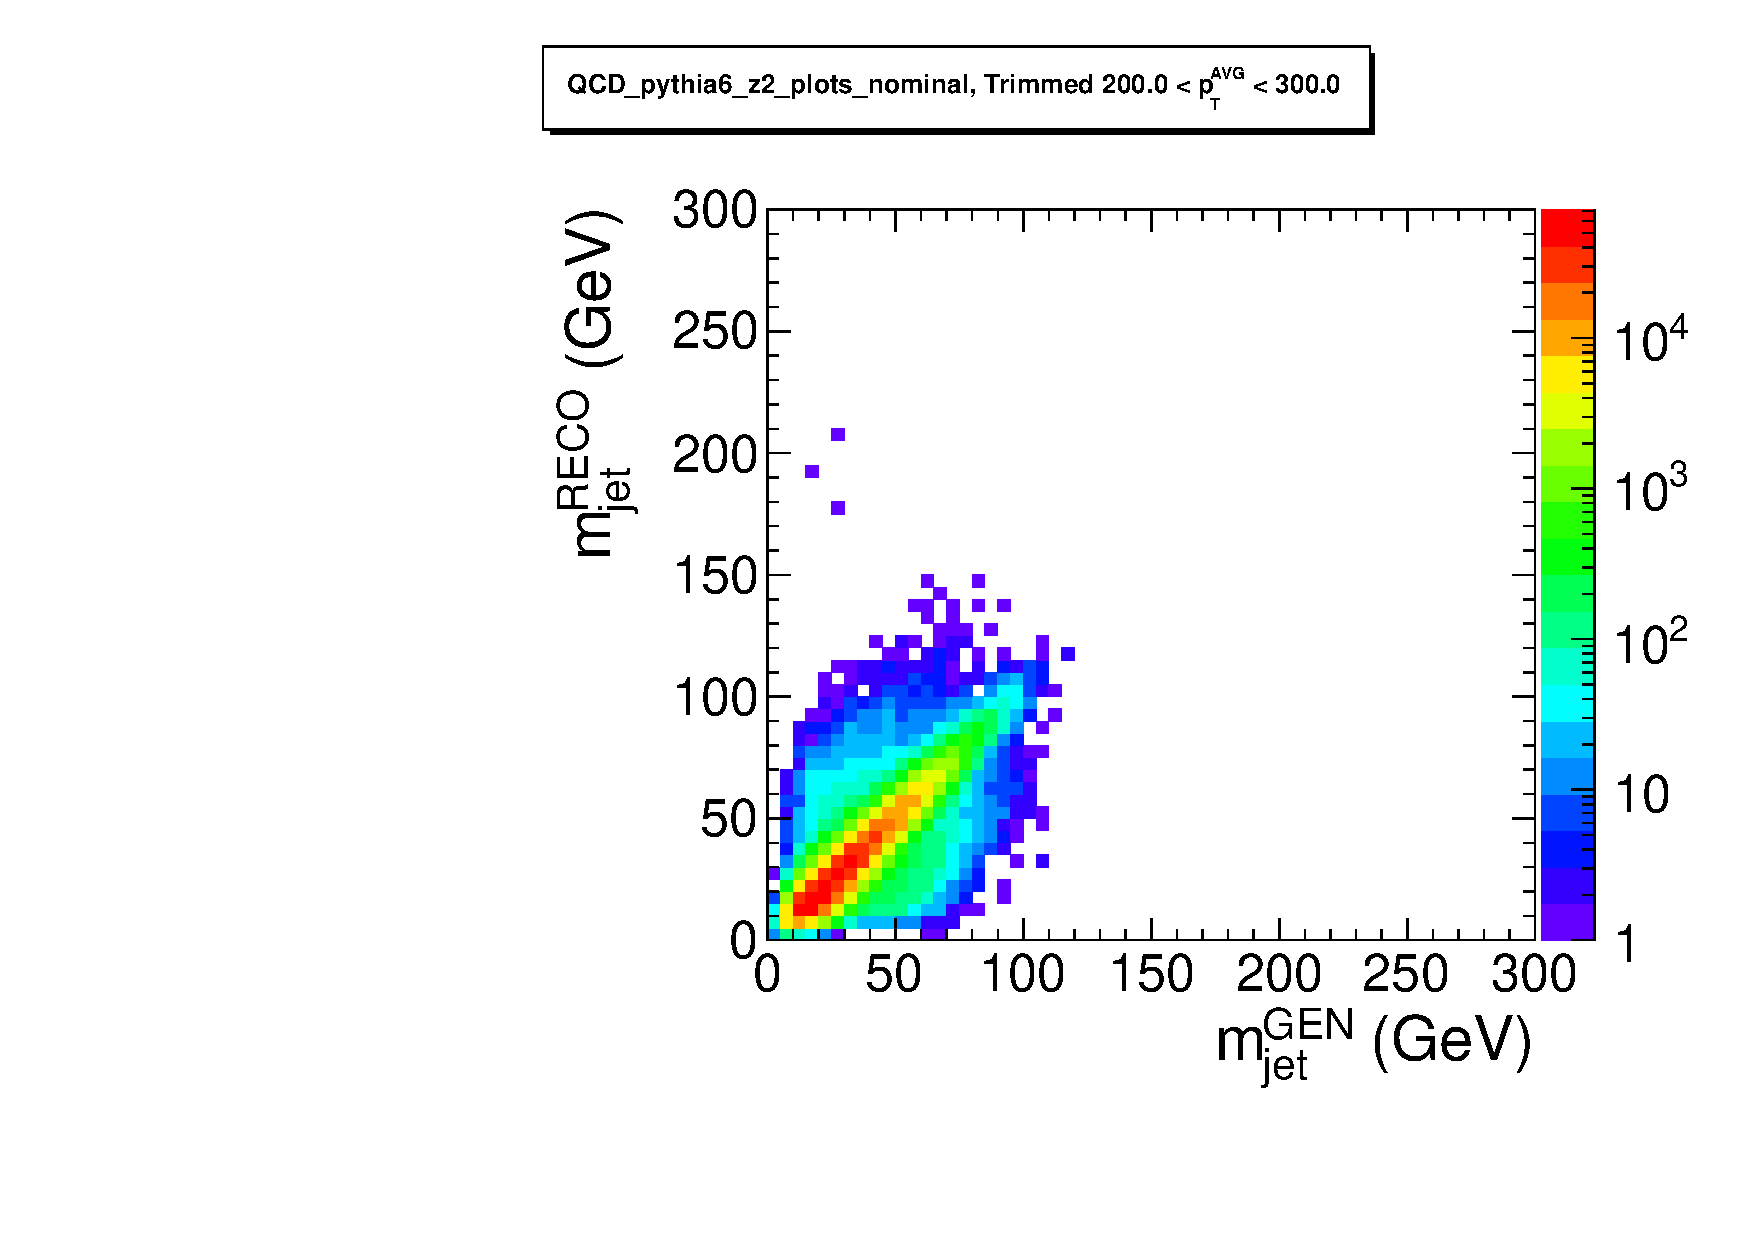
\includegraphics[width=0.3\textwidth]{figs/response_QCD_pythia6_z2_plots_nominal_Trimmed_pt3}}\\
\subfigure{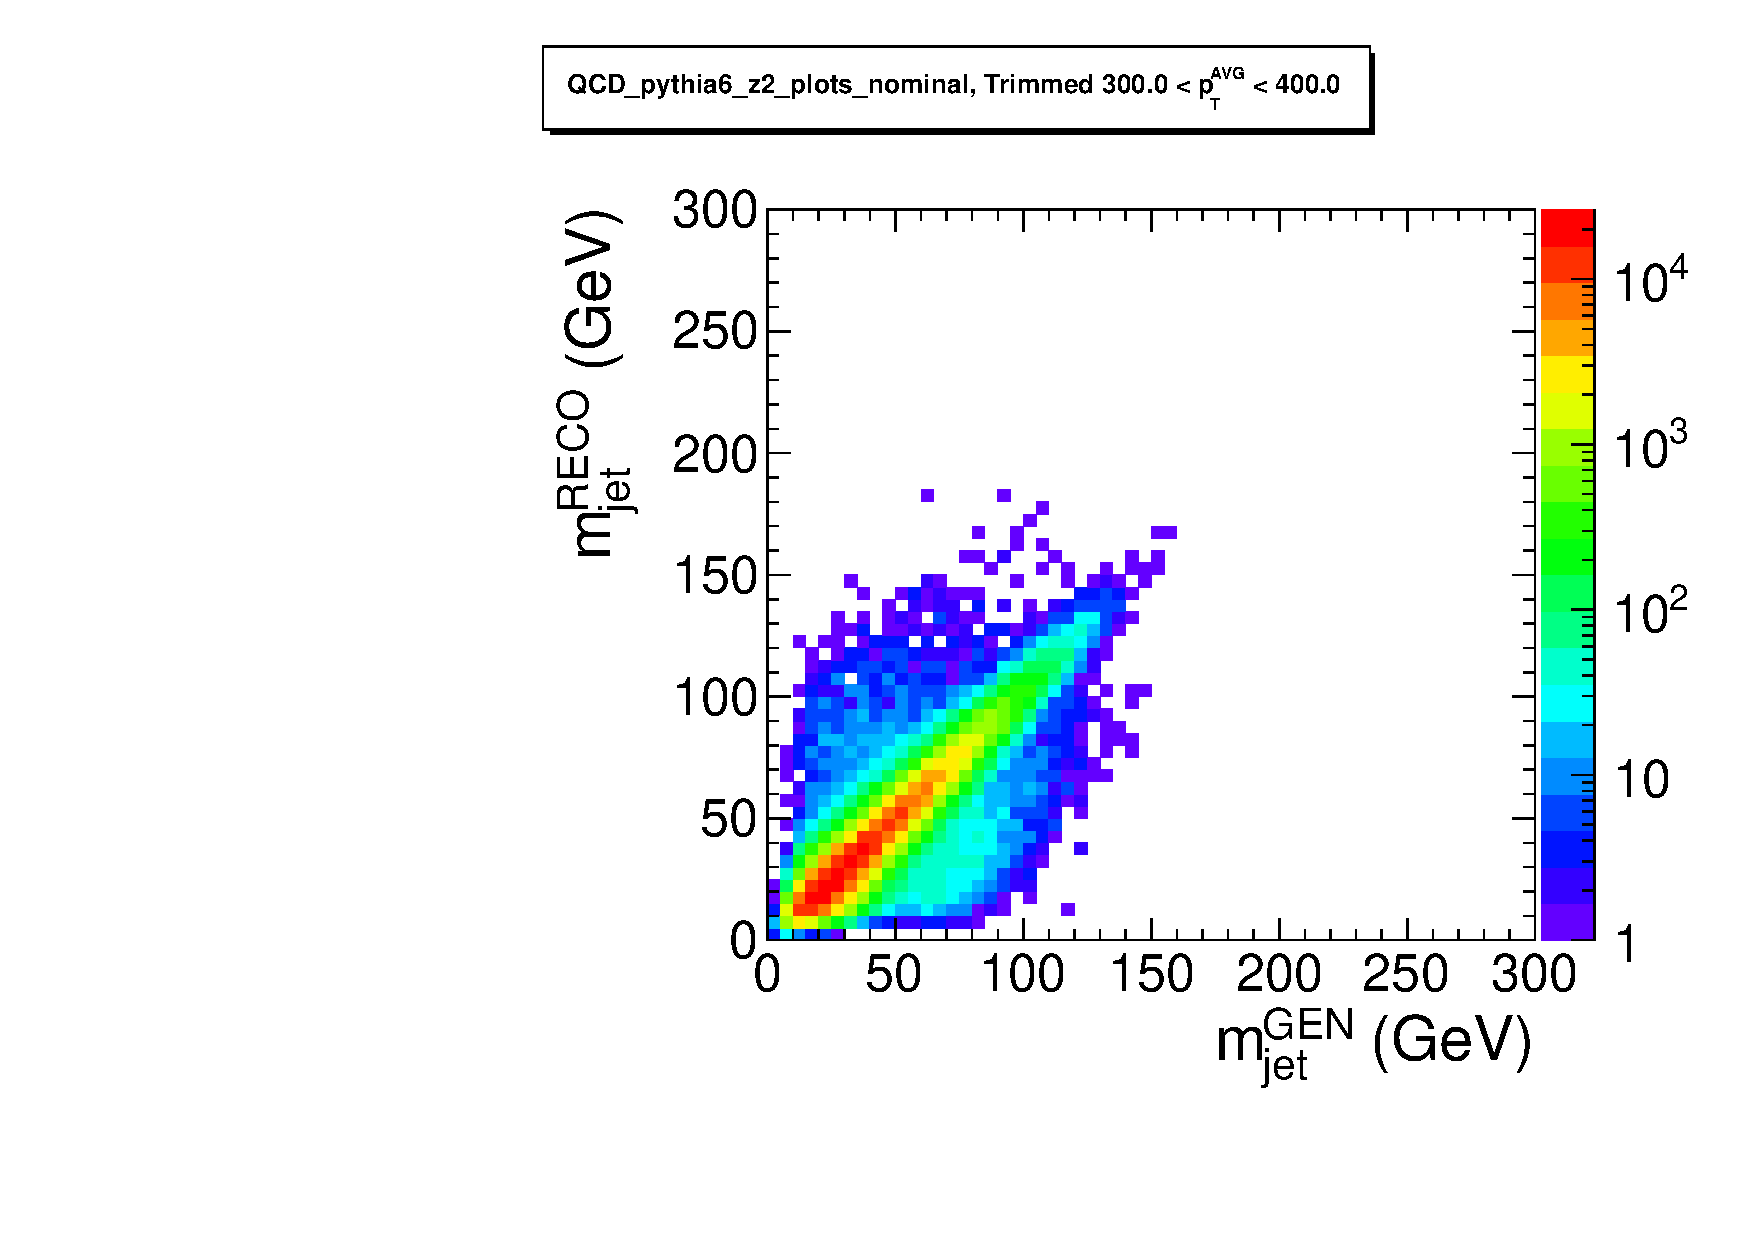
\includegraphics[width=0.3\textwidth]{figs/response_QCD_pythia6_z2_plots_nominal_Trimmed_pt4}}
\subfigure{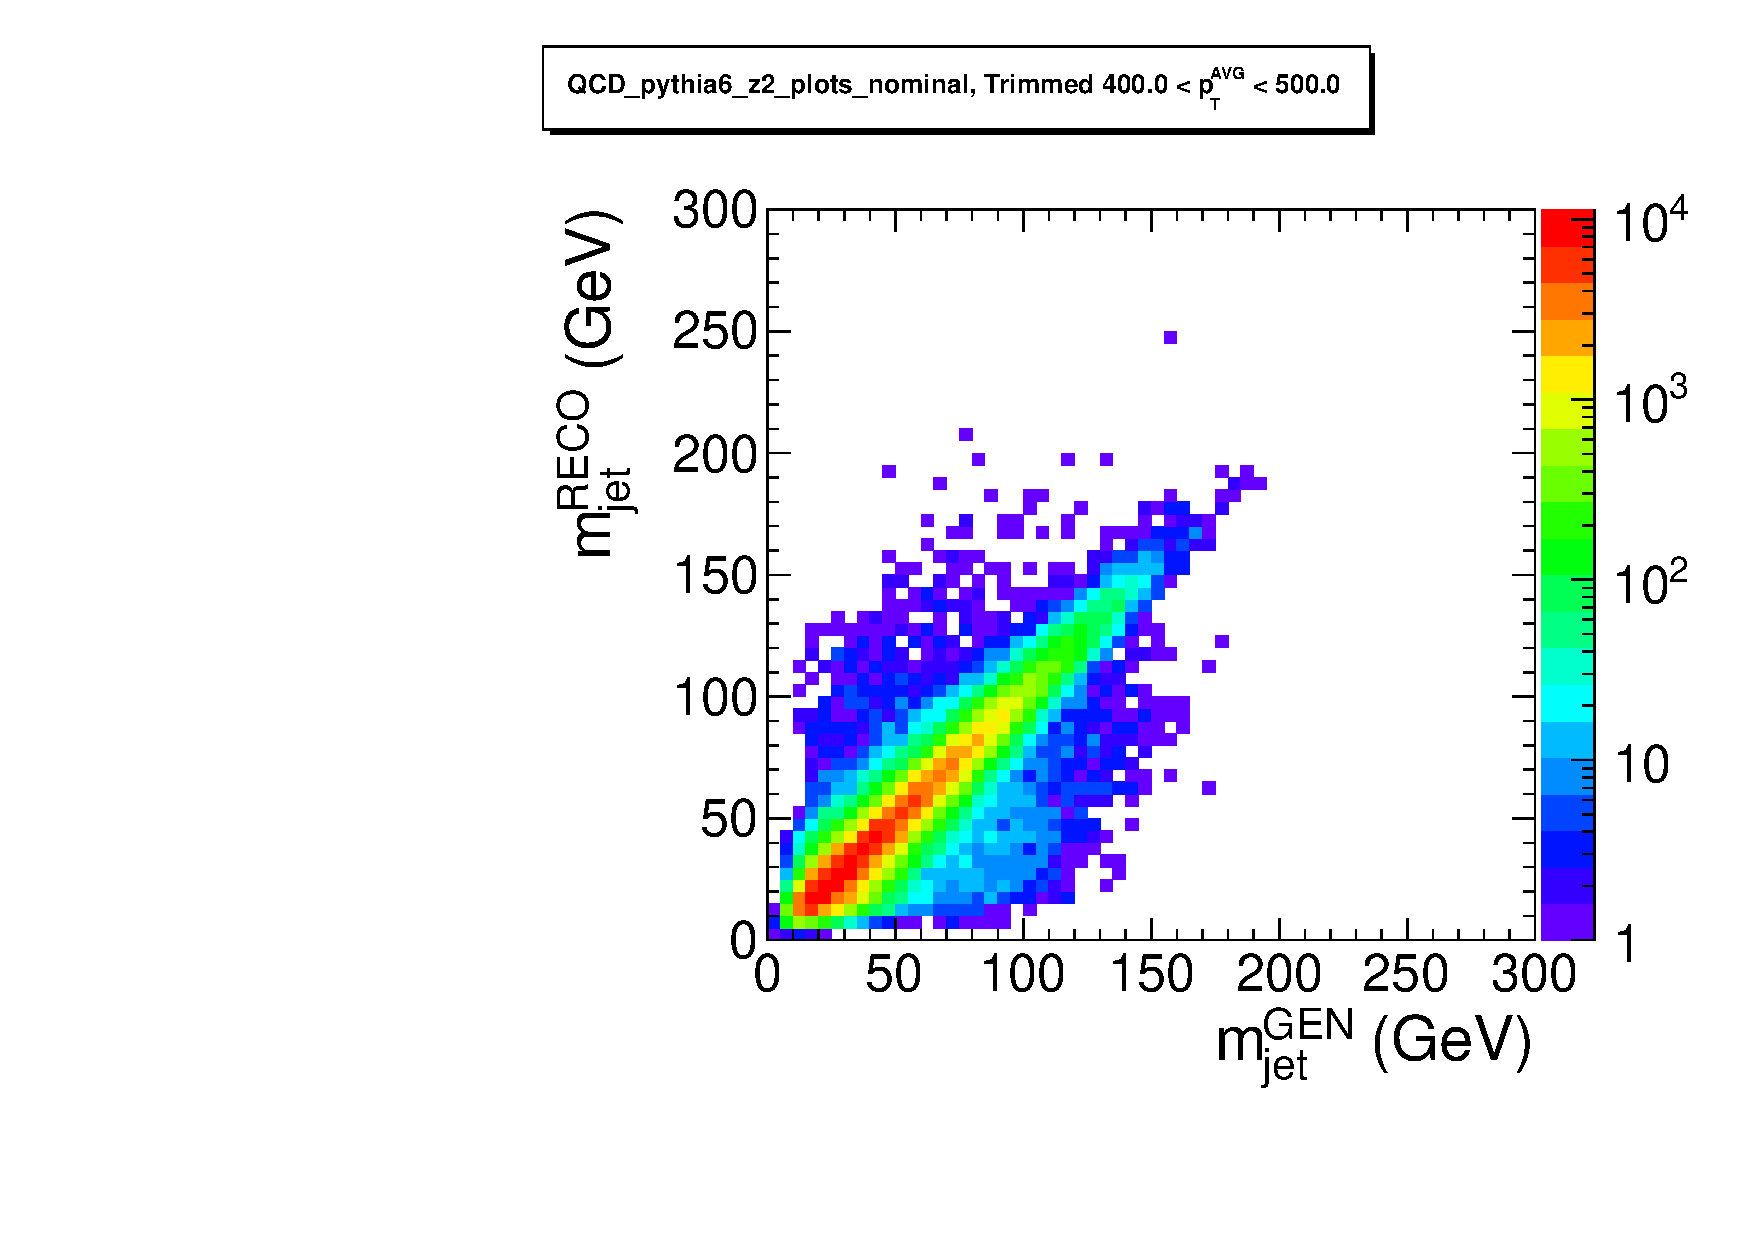
\includegraphics[width=0.3\textwidth]{figs/response_QCD_pythia6_z2_plots_nominal_Trimmed_pt5}}
\subfigure{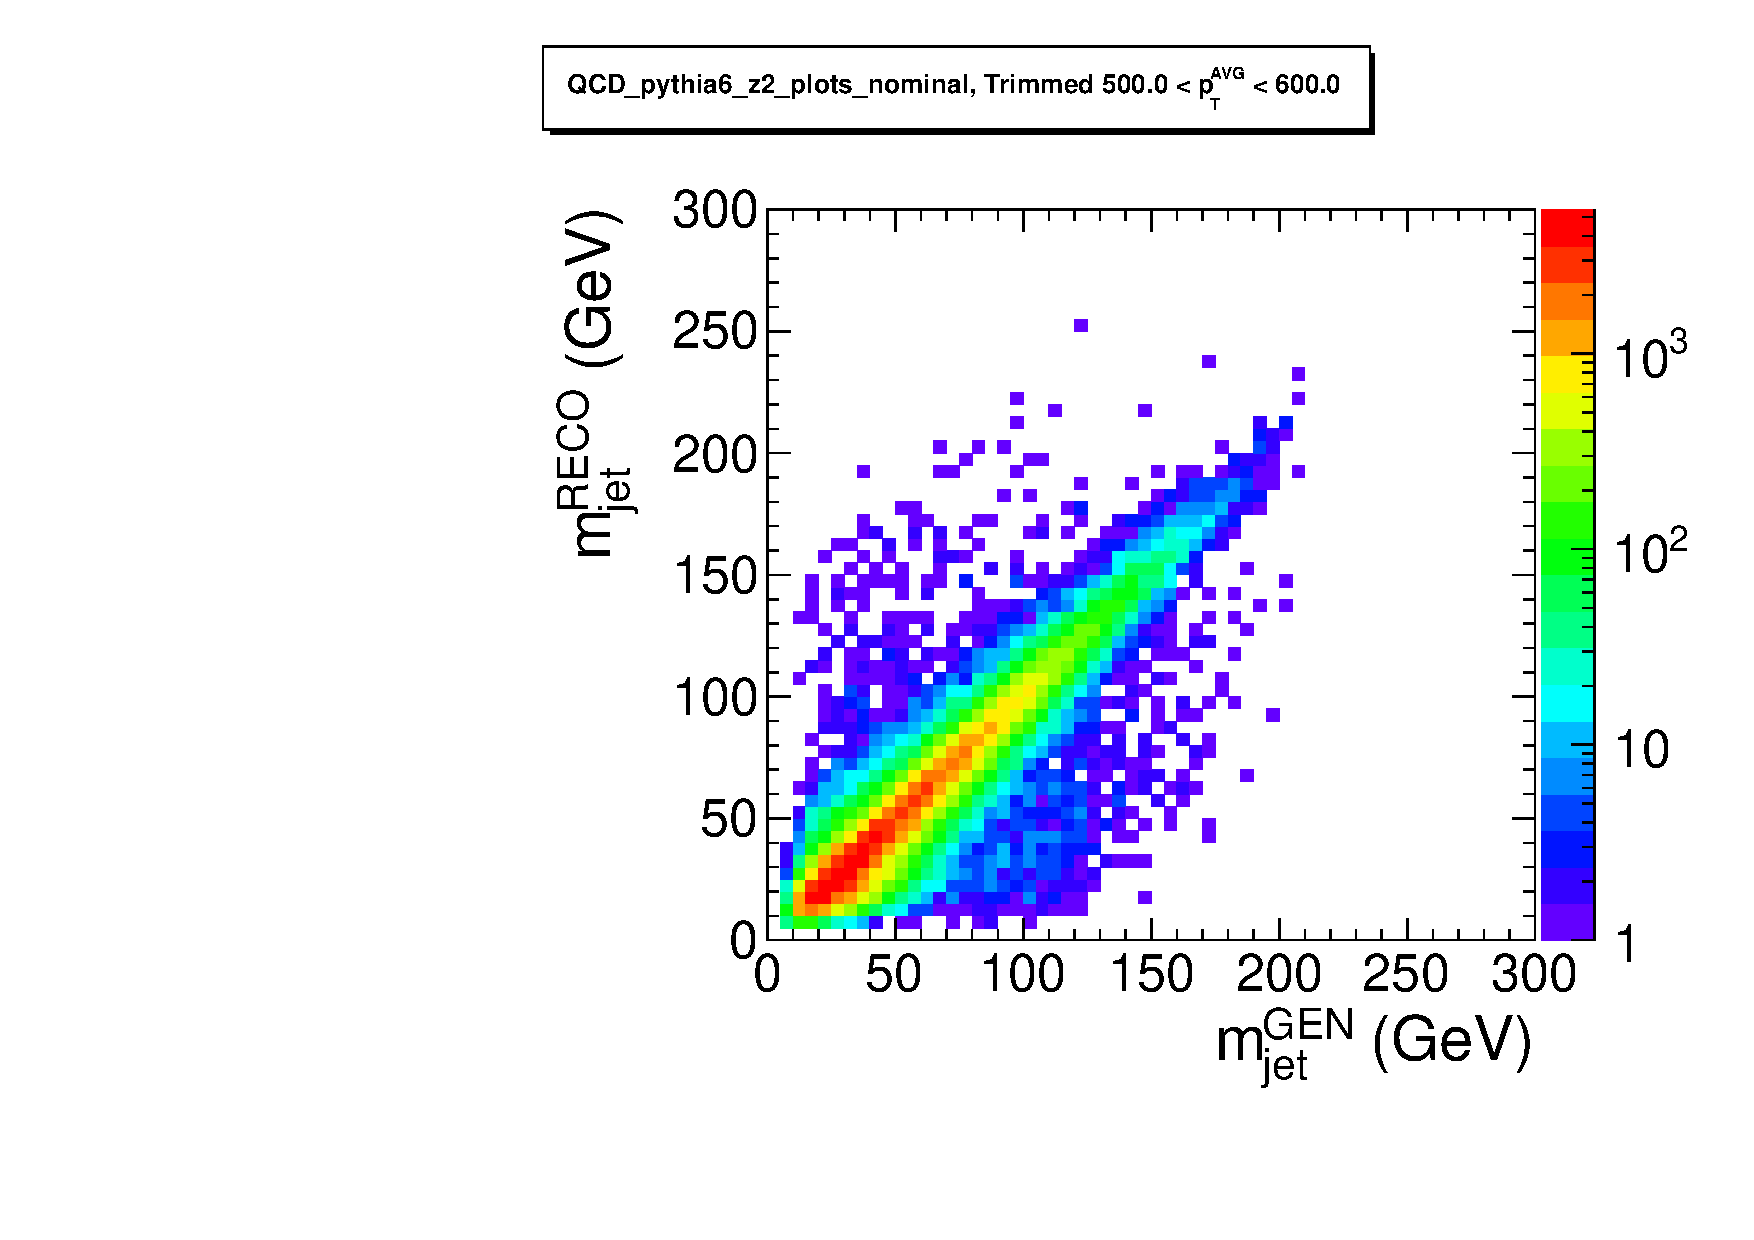
\includegraphics[width=0.3\textwidth]{figs/response_QCD_pythia6_z2_plots_nominal_Trimmed_pt6}}\\
\subfigure{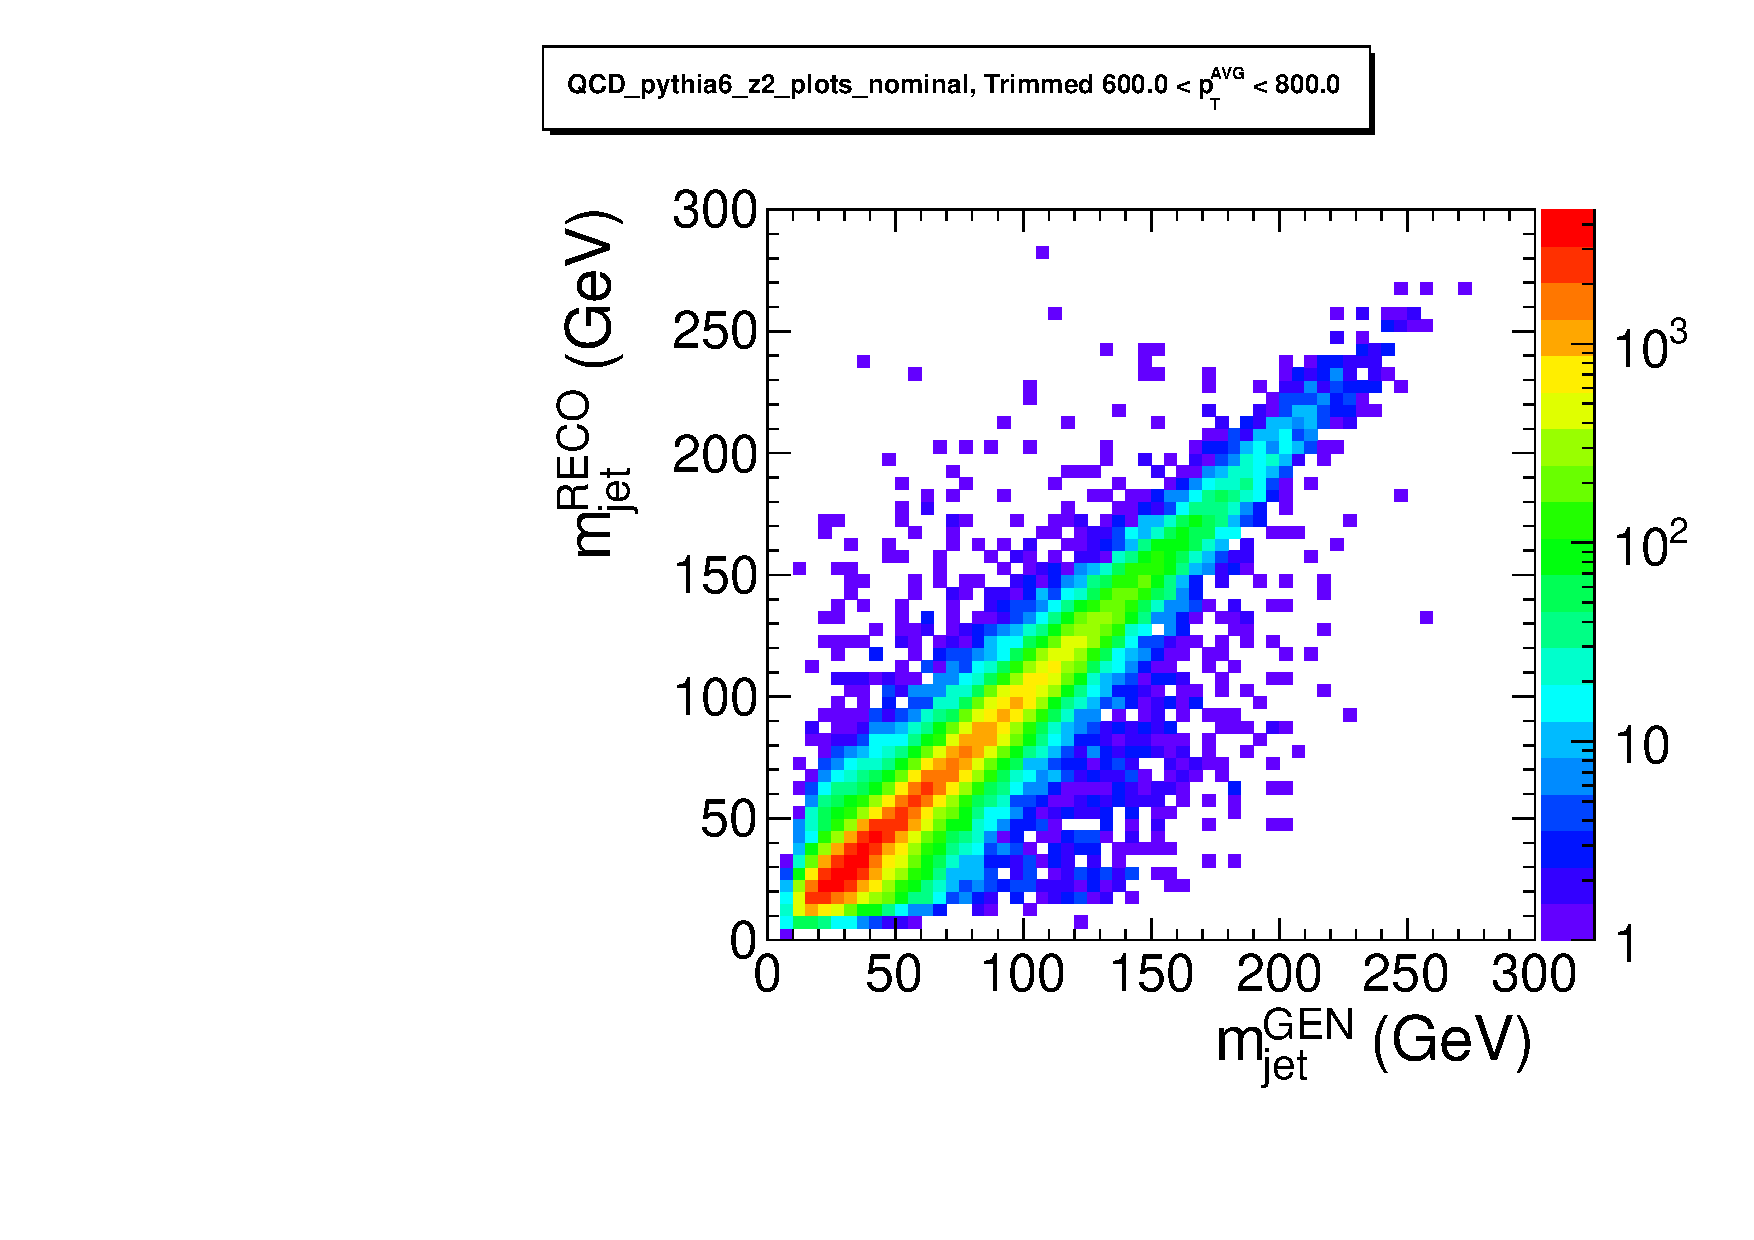
\includegraphics[width=0.3\textwidth]{figs/response_QCD_pythia6_z2_plots_nominal_Trimmed_pt7}}
\subfigure{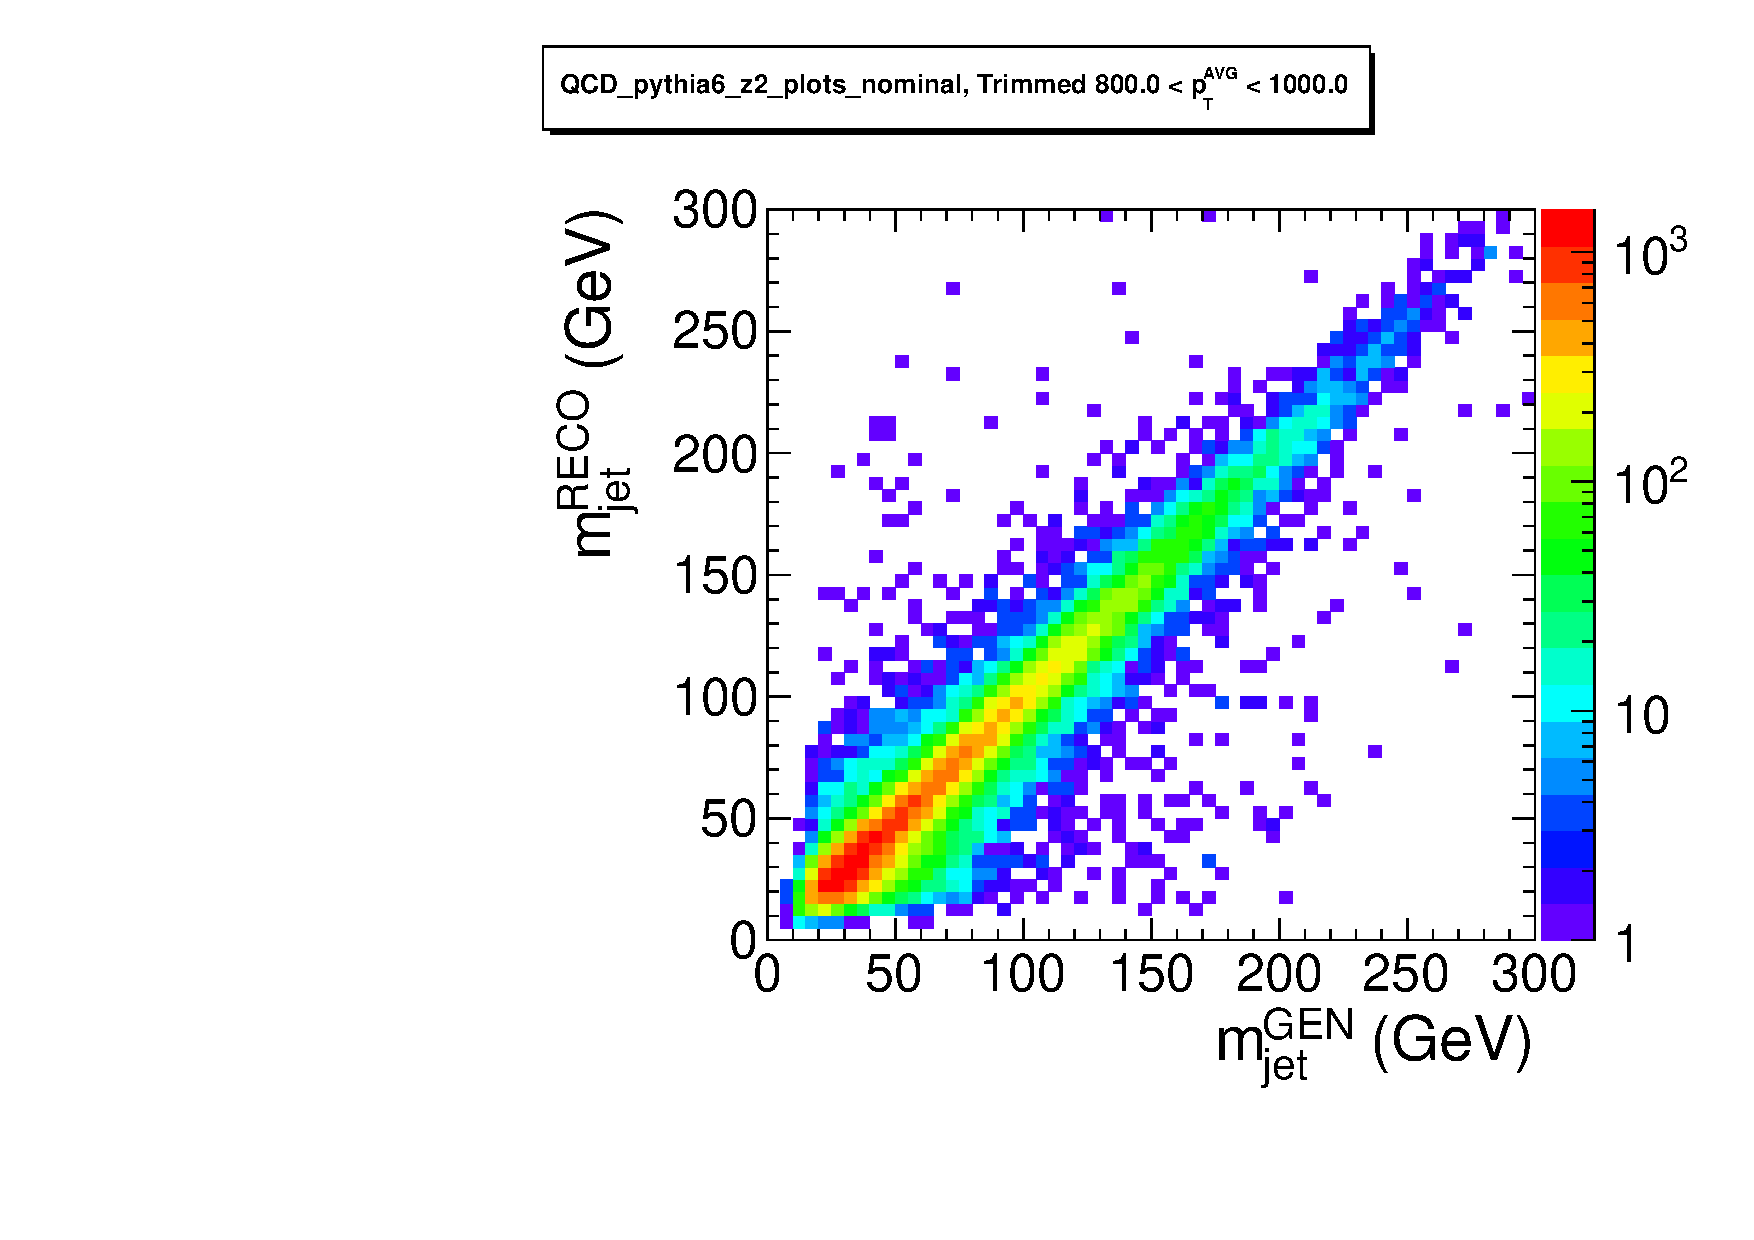
\includegraphics[width=0.3\textwidth]{figs/response_QCD_pythia6_z2_plots_nominal_Trimmed_pt8}}
\subfigure{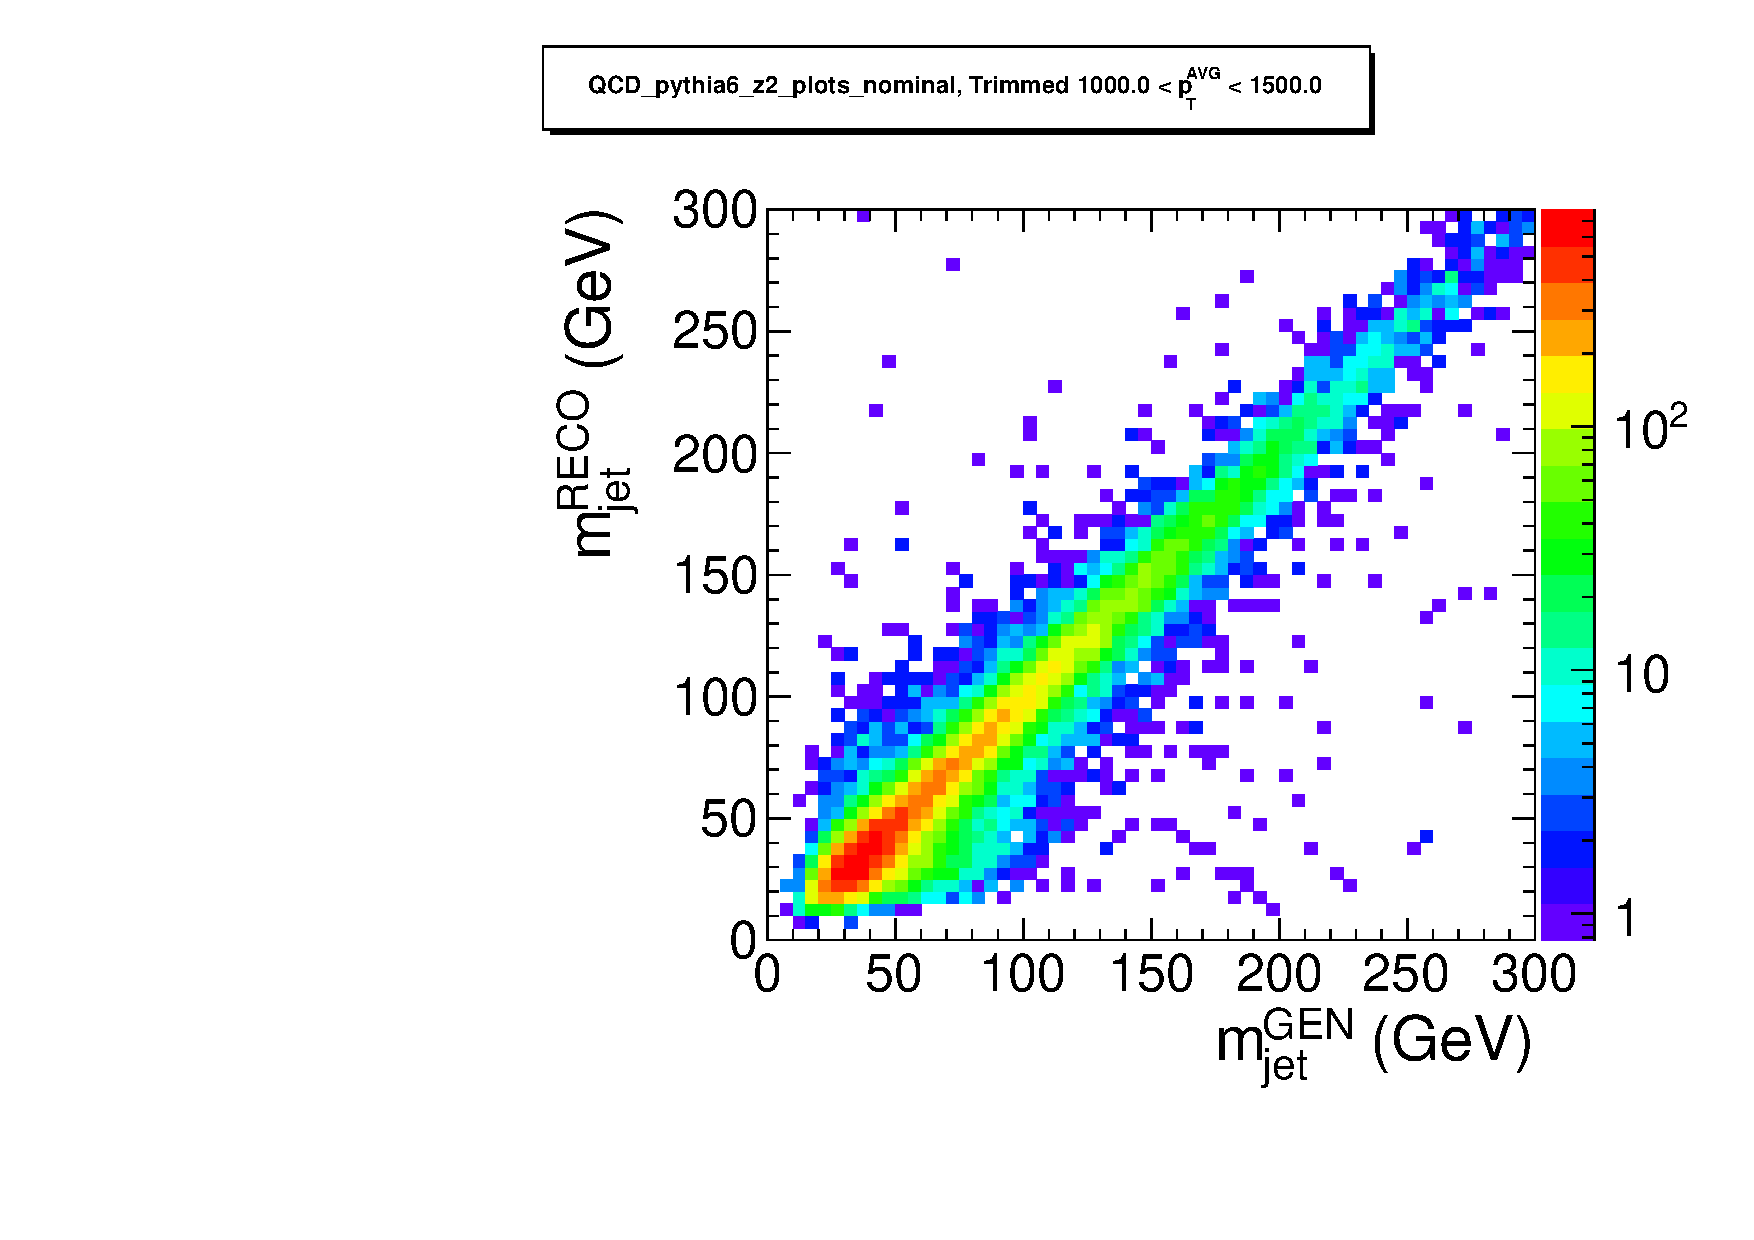
\includegraphics[width=0.3\textwidth]{figs/response_QCD_pythia6_z2_plots_nominal_Trimmed_pt9}}\\
\caption{Response of the jet mass for AK7 Trimmedjets,
for various $\pt^{AVG}$ bins. The true jet mass is shown
on the $x-$axis, and the reconstructed jet mass is shown on the
$y-$axis, using the \PYTHIA generator. 
\label{figs:response_QCD_pythia6_z2_plots_nominal_Trimmed_ptall}}
\end{figure}


\clearpage

\begin{figure}[htbp]
\centering
\subfigure{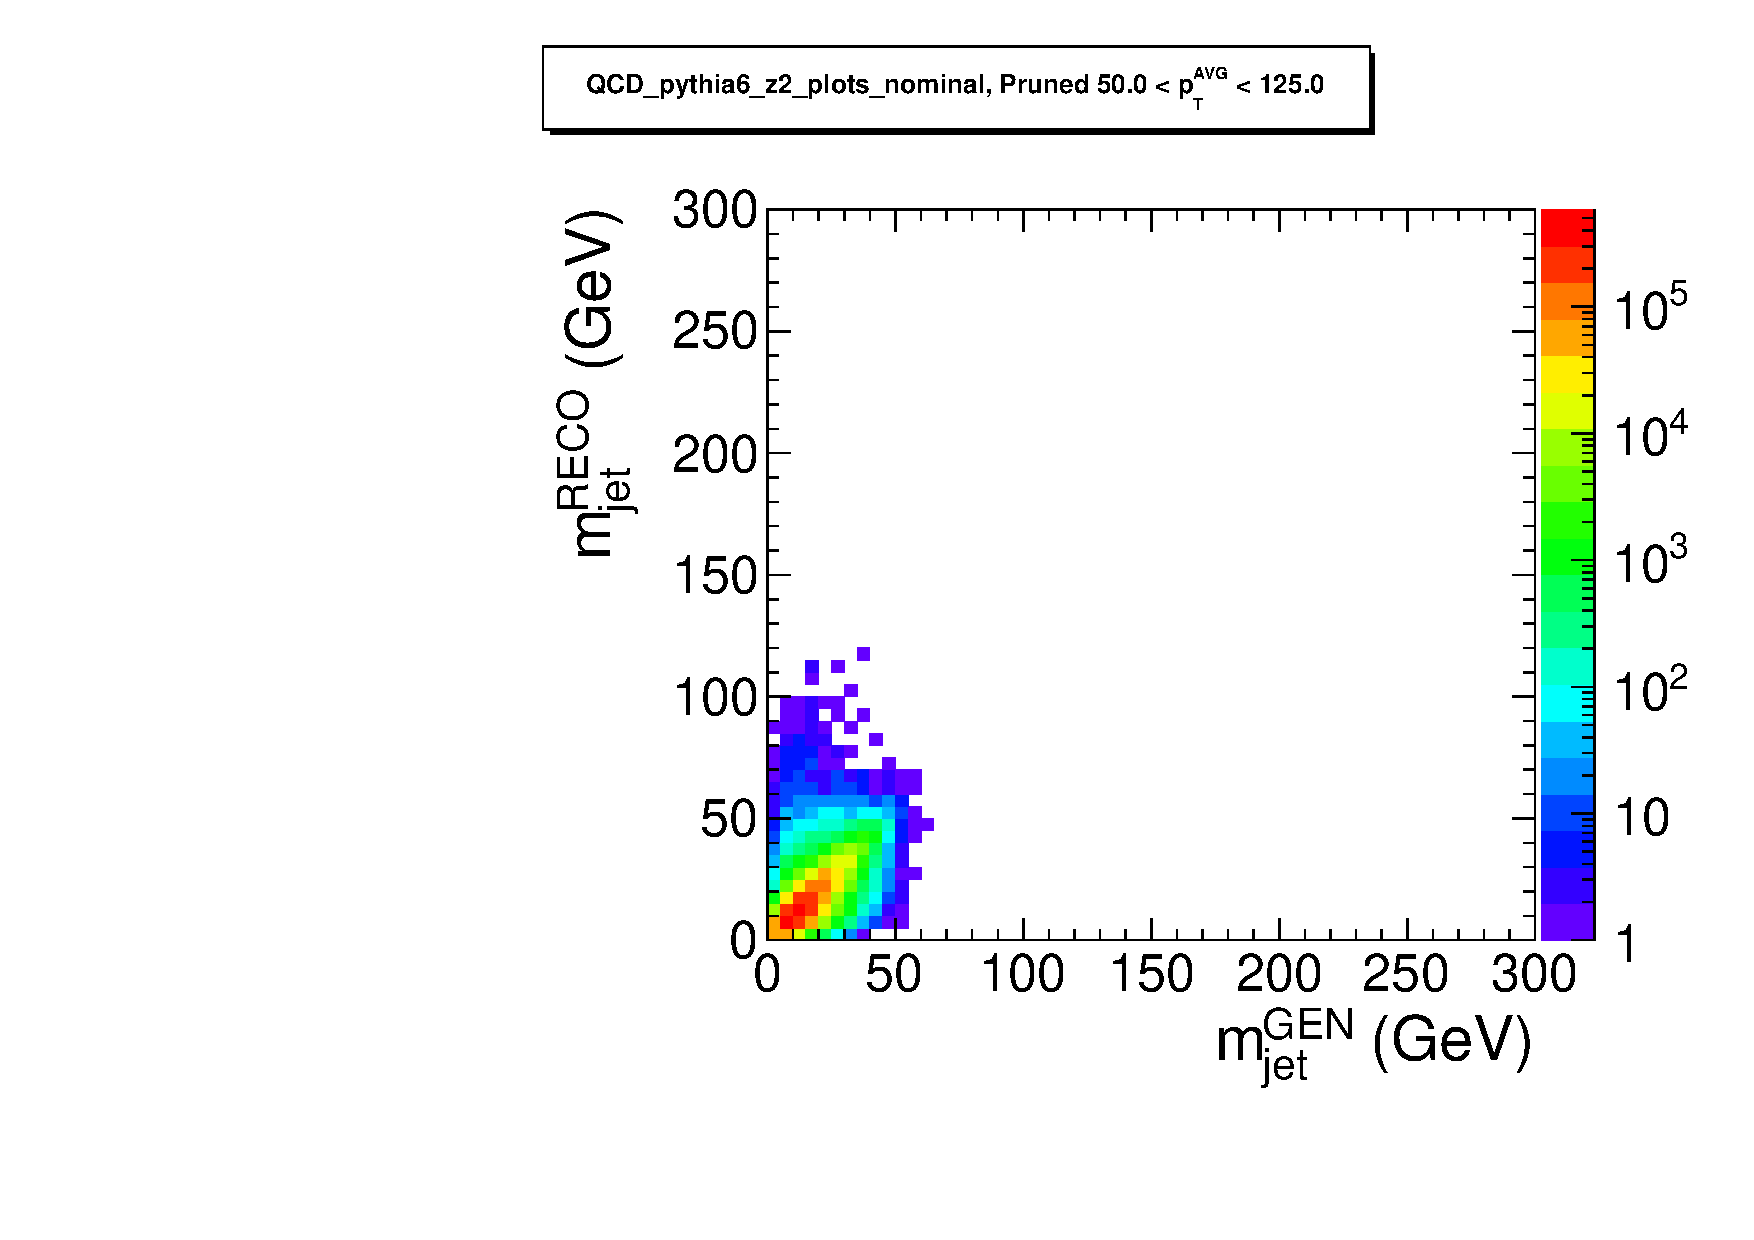
\includegraphics[width=0.3\textwidth]{figs/response_QCD_pythia6_z2_plots_nominal_Pruned_pt1}}
\subfigure{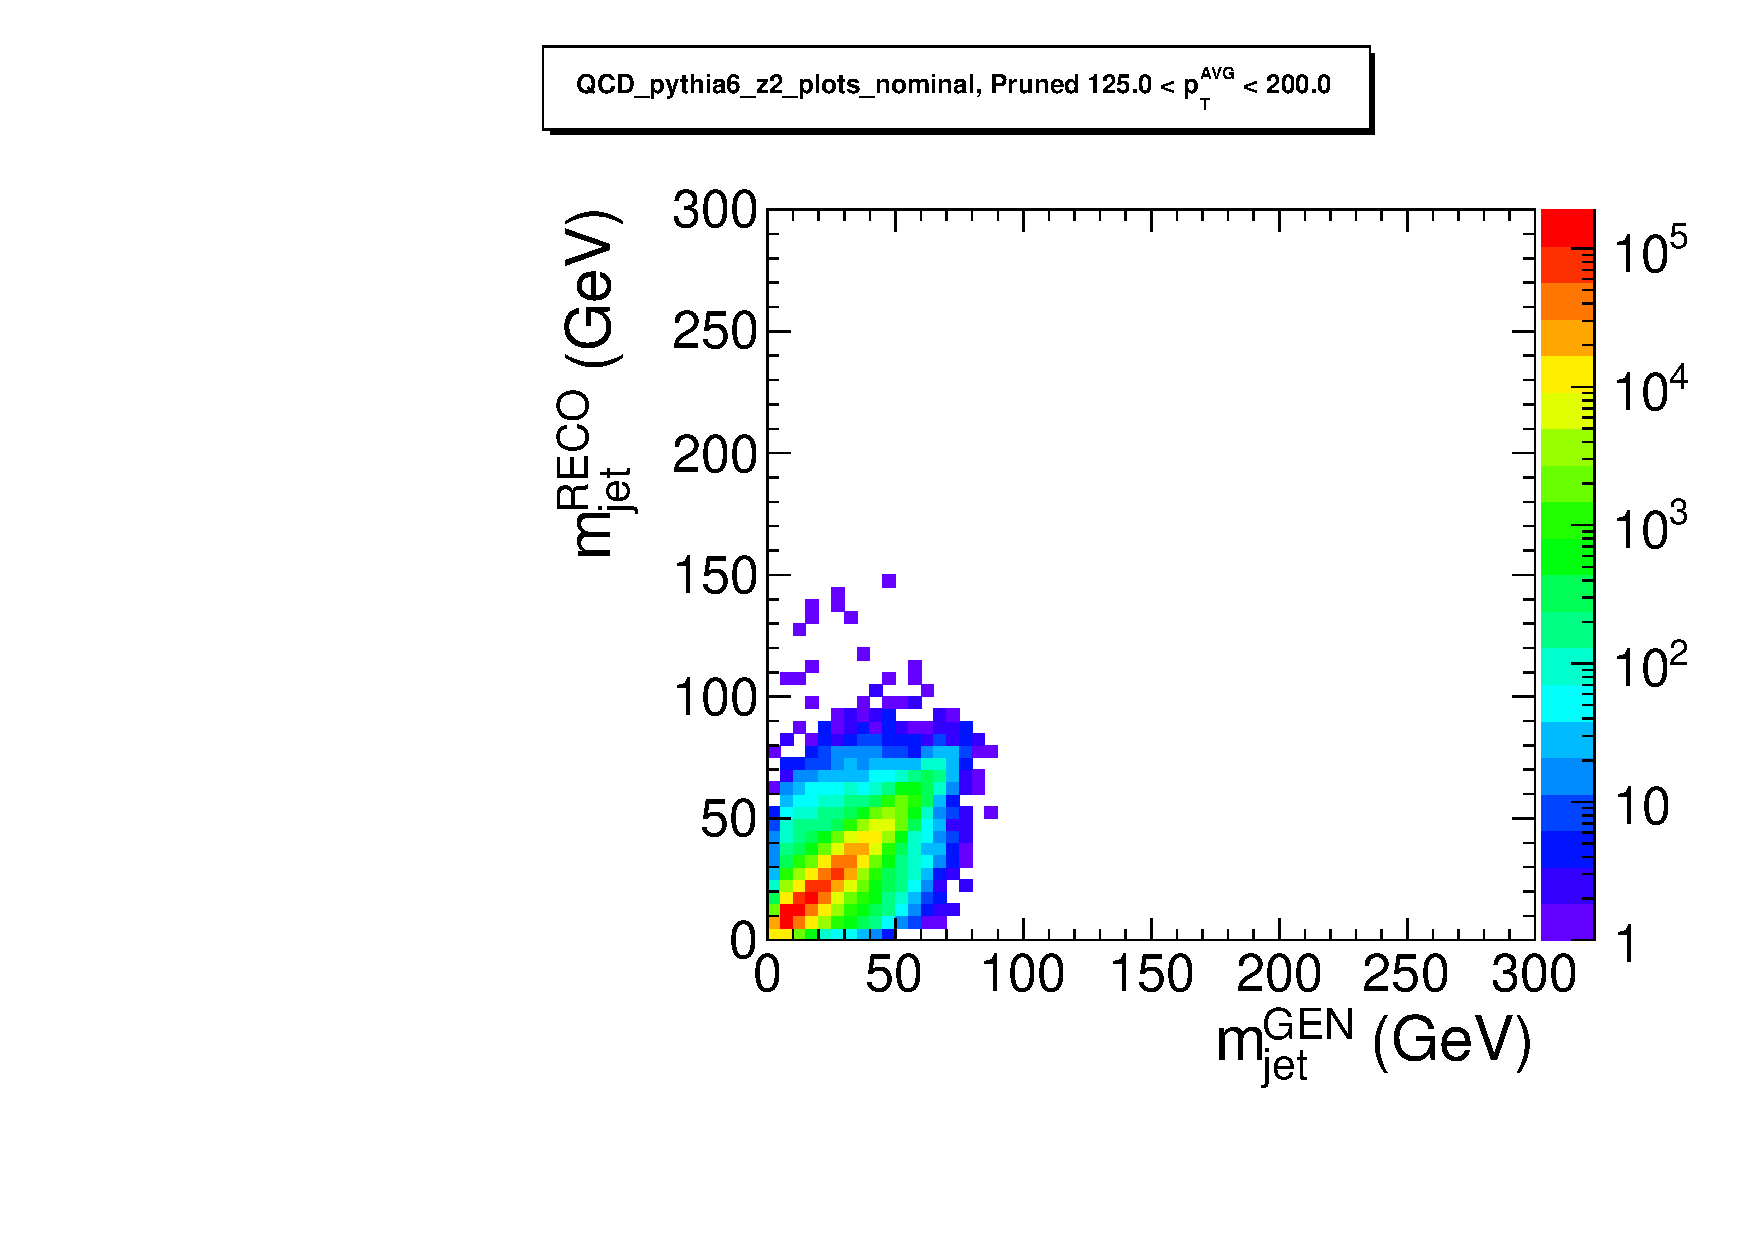
\includegraphics[width=0.3\textwidth]{figs/response_QCD_pythia6_z2_plots_nominal_Pruned_pt2}}
\subfigure{\includegraphics[width=0.3\textwidth]{figs/response_QCD_pythia6_z2_plots_nominal_Pruned_pt3}}\\
\subfigure{\includegraphics[width=0.3\textwidth]{figs/response_QCD_pythia6_z2_plots_nominal_Pruned_pt4}}
\subfigure{\includegraphics[width=0.3\textwidth]{figs/response_QCD_pythia6_z2_plots_nominal_Pruned_pt5}}
\subfigure{\includegraphics[width=0.3\textwidth]{figs/response_QCD_pythia6_z2_plots_nominal_Pruned_pt6}}\\
\subfigure{\includegraphics[width=0.3\textwidth]{figs/response_QCD_pythia6_z2_plots_nominal_Pruned_pt7}}
\subfigure{\includegraphics[width=0.3\textwidth]{figs/response_QCD_pythia6_z2_plots_nominal_Pruned_pt8}}
\subfigure{\includegraphics[width=0.3\textwidth]{figs/response_QCD_pythia6_z2_plots_nominal_Pruned_pt9}}\\
\caption{Response of the jet mass for AK7 Prunedjets,
for various $\pt^{AVG}$ bins. The true jet mass is shown
on the $x-$axis, and the reconstructed jet mass is shown on the
$y-$axis, using the \PYTHIA generator. 
\label{figs:response_QCD_pythia6_z2_plots_nominal_Pruned_ptall}}
\end{figure}


\clearpage

\begin{figure}[htbp]
\centering
\subfigure{\includegraphics[width=0.3\textwidth]{figs/response_QCD_pythia8_4c_plots_nominal_pt1}}
\subfigure{\includegraphics[width=0.3\textwidth]{figs/response_QCD_pythia8_4c_plots_nominal_pt2}}
\subfigure{\includegraphics[width=0.3\textwidth]{figs/response_QCD_pythia8_4c_plots_nominal_pt3}}\\
\subfigure{\includegraphics[width=0.3\textwidth]{figs/response_QCD_pythia8_4c_plots_nominal_pt4}}
\subfigure{\includegraphics[width=0.3\textwidth]{figs/response_QCD_pythia8_4c_plots_nominal_pt5}}
\subfigure{\includegraphics[width=0.3\textwidth]{figs/response_QCD_pythia8_4c_plots_nominal_pt6}}\\
\subfigure{\includegraphics[width=0.3\textwidth]{figs/response_QCD_pythia8_4c_plots_nominal_pt7}}
\subfigure{\includegraphics[width=0.3\textwidth]{figs/response_QCD_pythia8_4c_plots_nominal_pt8}}
\subfigure{\includegraphics[width=0.3\textwidth]{figs/response_QCD_pythia8_4c_plots_nominal_pt9}}\\
\caption{Response of the jet mass for AK7 jets,
for various $\pt^{AVG}$ bins. The true jet mass is shown
on the $x-$axis, and the reconstructed jet mass is shown on the
$y-$axis, using the \PYTHIAEIGHT generator. 
\label{figs:response_QCD_pythia8_4c_plots_nominal_ptall}}
\end{figure}


\clearpage

\begin{figure}[htbp]
\centering
\subfigure{\includegraphics[width=0.3\textwidth]{figs/response_QCD_pythia8_4c_plots_nominal_Filtered_pt1}}
\subfigure{\includegraphics[width=0.3\textwidth]{figs/response_QCD_pythia8_4c_plots_nominal_Filtered_pt2}}
\subfigure{\includegraphics[width=0.3\textwidth]{figs/response_QCD_pythia8_4c_plots_nominal_Filtered_pt3}}\\
\subfigure{\includegraphics[width=0.3\textwidth]{figs/response_QCD_pythia8_4c_plots_nominal_Filtered_pt4}}
\subfigure{\includegraphics[width=0.3\textwidth]{figs/response_QCD_pythia8_4c_plots_nominal_Filtered_pt5}}
\subfigure{\includegraphics[width=0.3\textwidth]{figs/response_QCD_pythia8_4c_plots_nominal_Filtered_pt6}}\\
\subfigure{\includegraphics[width=0.3\textwidth]{figs/response_QCD_pythia8_4c_plots_nominal_Filtered_pt7}}
\subfigure{\includegraphics[width=0.3\textwidth]{figs/response_QCD_pythia8_4c_plots_nominal_Filtered_pt8}}
\subfigure{\includegraphics[width=0.3\textwidth]{figs/response_QCD_pythia8_4c_plots_nominal_Filtered_pt9}}\\
\caption{Response of the jet mass for AK7 Filteredjets,
for various $\pt^{AVG}$ bins. The true jet mass is shown
on the $x-$axis, and the reconstructed jet mass is shown on the
$y-$axis, using the \PYTHIAEIGHT generator. 
\label{figs:response_QCD_pythia8_4c_plots_nominal_Filtered_ptall}}
\end{figure}


\clearpage

\begin{figure}[htbp]
\centering
\subfigure{\includegraphics[width=0.3\textwidth]{figs/response_QCD_pythia8_4c_plots_nominal_Trimmed_pt1}}
\subfigure{\includegraphics[width=0.3\textwidth]{figs/response_QCD_pythia8_4c_plots_nominal_Trimmed_pt2}}
\subfigure{\includegraphics[width=0.3\textwidth]{figs/response_QCD_pythia8_4c_plots_nominal_Trimmed_pt3}}\\
\subfigure{\includegraphics[width=0.3\textwidth]{figs/response_QCD_pythia8_4c_plots_nominal_Trimmed_pt4}}
\subfigure{\includegraphics[width=0.3\textwidth]{figs/response_QCD_pythia8_4c_plots_nominal_Trimmed_pt5}}
\subfigure{\includegraphics[width=0.3\textwidth]{figs/response_QCD_pythia8_4c_plots_nominal_Trimmed_pt6}}\\
\subfigure{\includegraphics[width=0.3\textwidth]{figs/response_QCD_pythia8_4c_plots_nominal_Trimmed_pt7}}
\subfigure{\includegraphics[width=0.3\textwidth]{figs/response_QCD_pythia8_4c_plots_nominal_Trimmed_pt8}}
\subfigure{\includegraphics[width=0.3\textwidth]{figs/response_QCD_pythia8_4c_plots_nominal_Trimmed_pt9}}\\
\caption{Response of the jet mass for AK7 Trimmedjets,
for various $\pt^{AVG}$ bins. The true jet mass is shown
on the $x-$axis, and the reconstructed jet mass is shown on the
$y-$axis, using the \PYTHIAEIGHT generator. 
\label{figs:response_QCD_pythia8_4c_plots_nominal_Trimmed_ptall}}
\end{figure}


\clearpage

\begin{figure}[htbp]
\centering
\subfigure{\includegraphics[width=0.3\textwidth]{figs/response_QCD_pythia8_4c_plots_nominal_Pruned_pt1}}
\subfigure{\includegraphics[width=0.3\textwidth]{figs/response_QCD_pythia8_4c_plots_nominal_Pruned_pt2}}
\subfigure{\includegraphics[width=0.3\textwidth]{figs/response_QCD_pythia8_4c_plots_nominal_Pruned_pt3}}\\
\subfigure{\includegraphics[width=0.3\textwidth]{figs/response_QCD_pythia8_4c_plots_nominal_Pruned_pt4}}
\subfigure{\includegraphics[width=0.3\textwidth]{figs/response_QCD_pythia8_4c_plots_nominal_Pruned_pt5}}
\subfigure{\includegraphics[width=0.3\textwidth]{figs/response_QCD_pythia8_4c_plots_nominal_Pruned_pt6}}\\
\subfigure{\includegraphics[width=0.3\textwidth]{figs/response_QCD_pythia8_4c_plots_nominal_Pruned_pt7}}
\subfigure{\includegraphics[width=0.3\textwidth]{figs/response_QCD_pythia8_4c_plots_nominal_Pruned_pt8}}
\subfigure{\includegraphics[width=0.3\textwidth]{figs/response_QCD_pythia8_4c_plots_nominal_Pruned_pt9}}\\
\caption{Response of the jet mass for AK7 Prunedjets,
for various $\pt^{AVG}$ bins. The true jet mass is shown
on the $x-$axis, and the reconstructed jet mass is shown on the
$y-$axis, using the \PYTHIAEIGHT generator. 
\label{figs:response_QCD_pythia8_4c_plots_nominal_Pruned_ptall}}
\end{figure}


\clearpage

\begin{figure}[htbp]
\centering
\subfigure{\includegraphics[width=0.3\textwidth]{figs/response_QCD_herwigpp_23_plots_nominal_pt1}}
\subfigure{\includegraphics[width=0.3\textwidth]{figs/response_QCD_herwigpp_23_plots_nominal_pt2}}
\subfigure{\includegraphics[width=0.3\textwidth]{figs/response_QCD_herwigpp_23_plots_nominal_pt3}}\\
\subfigure{\includegraphics[width=0.3\textwidth]{figs/response_QCD_herwigpp_23_plots_nominal_pt4}}
\subfigure{\includegraphics[width=0.3\textwidth]{figs/response_QCD_herwigpp_23_plots_nominal_pt5}}
\subfigure{\includegraphics[width=0.3\textwidth]{figs/response_QCD_herwigpp_23_plots_nominal_pt6}}\\
\subfigure{\includegraphics[width=0.3\textwidth]{figs/response_QCD_herwigpp_23_plots_nominal_pt7}}
\subfigure{\includegraphics[width=0.3\textwidth]{figs/response_QCD_herwigpp_23_plots_nominal_pt8}}
\subfigure{\includegraphics[width=0.3\textwidth]{figs/response_QCD_herwigpp_23_plots_nominal_pt9}}\\
\caption{Response of the jet mass for AK7 jets,
for various $\pt^{AVG}$ bins. The true jet mass is shown
on the $x-$axis, and the reconstructed jet mass is shown on the
$y-$axis, using the \HERWIG generator. 
\label{figs:response_QCD_herwigpp_23_plots_nominal_ptall}}
\end{figure}


\clearpage

\begin{figure}[htbp]
\centering
\subfigure{\includegraphics[width=0.3\textwidth]{figs/response_QCD_herwigpp_23_plots_nominal_Filtered_pt1}}
\subfigure{\includegraphics[width=0.3\textwidth]{figs/response_QCD_herwigpp_23_plots_nominal_Filtered_pt2}}
\subfigure{\includegraphics[width=0.3\textwidth]{figs/response_QCD_herwigpp_23_plots_nominal_Filtered_pt3}}\\
\subfigure{\includegraphics[width=0.3\textwidth]{figs/response_QCD_herwigpp_23_plots_nominal_Filtered_pt4}}
\subfigure{\includegraphics[width=0.3\textwidth]{figs/response_QCD_herwigpp_23_plots_nominal_Filtered_pt5}}
\subfigure{\includegraphics[width=0.3\textwidth]{figs/response_QCD_herwigpp_23_plots_nominal_Filtered_pt6}}\\
\subfigure{\includegraphics[width=0.3\textwidth]{figs/response_QCD_herwigpp_23_plots_nominal_Filtered_pt7}}
\subfigure{\includegraphics[width=0.3\textwidth]{figs/response_QCD_herwigpp_23_plots_nominal_Filtered_pt8}}
\subfigure{\includegraphics[width=0.3\textwidth]{figs/response_QCD_herwigpp_23_plots_nominal_Filtered_pt9}}\\
\caption{Response of the jet mass for AK7 Filteredjets,
for various $\pt^{AVG}$ bins. The true jet mass is shown
on the $x-$axis, and the reconstructed jet mass is shown on the
$y-$axis, using the \HERWIG generator. 
\label{figs:response_QCD_herwigpp_23_plots_nominal_Filtered_ptall}}
\end{figure}


\clearpage

\begin{figure}[htbp]
\centering
\subfigure{\includegraphics[width=0.3\textwidth]{figs/response_QCD_herwigpp_23_plots_nominal_Trimmed_pt1}}
\subfigure{\includegraphics[width=0.3\textwidth]{figs/response_QCD_herwigpp_23_plots_nominal_Trimmed_pt2}}
\subfigure{\includegraphics[width=0.3\textwidth]{figs/response_QCD_herwigpp_23_plots_nominal_Trimmed_pt3}}\\
\subfigure{\includegraphics[width=0.3\textwidth]{figs/response_QCD_herwigpp_23_plots_nominal_Trimmed_pt4}}
\subfigure{\includegraphics[width=0.3\textwidth]{figs/response_QCD_herwigpp_23_plots_nominal_Trimmed_pt5}}
\subfigure{\includegraphics[width=0.3\textwidth]{figs/response_QCD_herwigpp_23_plots_nominal_Trimmed_pt6}}\\
\subfigure{\includegraphics[width=0.3\textwidth]{figs/response_QCD_herwigpp_23_plots_nominal_Trimmed_pt7}}
\subfigure{\includegraphics[width=0.3\textwidth]{figs/response_QCD_herwigpp_23_plots_nominal_Trimmed_pt8}}
\subfigure{\includegraphics[width=0.3\textwidth]{figs/response_QCD_herwigpp_23_plots_nominal_Trimmed_pt9}}\\
\caption{Response of the jet mass for AK7 Trimmedjets,
for various $\pt^{AVG}$ bins. The true jet mass is shown
on the $x-$axis, and the reconstructed jet mass is shown on the
$y-$axis, using the \HERWIG generator. 
\label{figs:response_QCD_herwigpp_23_plots_nominal_Trimmed_ptall}}
\end{figure}


\clearpage

\begin{figure}[htbp]
\centering
\subfigure{\includegraphics[width=0.3\textwidth]{figs/response_QCD_herwigpp_23_plots_nominal_Pruned_pt1}}
\subfigure{\includegraphics[width=0.3\textwidth]{figs/response_QCD_herwigpp_23_plots_nominal_Pruned_pt2}}
\subfigure{\includegraphics[width=0.3\textwidth]{figs/response_QCD_herwigpp_23_plots_nominal_Pruned_pt3}}\\
\subfigure{\includegraphics[width=0.3\textwidth]{figs/response_QCD_herwigpp_23_plots_nominal_Pruned_pt4}}
\subfigure{\includegraphics[width=0.3\textwidth]{figs/response_QCD_herwigpp_23_plots_nominal_Pruned_pt5}}
\subfigure{\includegraphics[width=0.3\textwidth]{figs/response_QCD_herwigpp_23_plots_nominal_Pruned_pt6}}\\
\subfigure{\includegraphics[width=0.3\textwidth]{figs/response_QCD_herwigpp_23_plots_nominal_Pruned_pt7}}
\subfigure{\includegraphics[width=0.3\textwidth]{figs/response_QCD_herwigpp_23_plots_nominal_Pruned_pt8}}
\subfigure{\includegraphics[width=0.3\textwidth]{figs/response_QCD_herwigpp_23_plots_nominal_Pruned_pt9}}\\
\caption{Response of the jet mass for AK7 Prunedjets,
for various $\pt^{AVG}$ bins. The true jet mass is shown
on the $x-$axis, and the reconstructed jet mass is shown on the
$y-$axis, using the \HERWIG generator. 
\label{figs:response_QCD_herwigpp_23_plots_nominal_Pruned_ptall}}
\end{figure}


\clearpage


\clearpage

\subsection{Closure test}

\label{sec:closure}

The unfolding procedure we have used makes an assumption that
the dijet events that we are using are the same at the detector
level and the generator level. Furthermore, the jet algorithm
itself is an arbitrary designation of the event, and what to
call a ``jet'' depends on the energy scale of the process.
For these reasons, the assumed dijet topology as described
above may not correspond to the true topology of the event.
Trijet events (and quadjet, etc) can pollute the dijet
events, even with a veto on extra jet activity. This is 
particularly problematic at lower $\pt$. Hence, a critical test
is the closure of our unfolding procedure. That is,
the MC is taken as both the input to the response matrix,
and as simulated ``data'', and compared to the MC true
distribution at the generator level. Any discrepancy here
is a problem with the assumption of the dijet topology.

Figures~\ref{figs:unfoldedMeasurementDijets_1_closuretest}-
\ref{figs:unfoldedMeasurementDijets_9_closuretest}
show the closure test for the various $\pt^{AVG}$ bins
in the sample. Here, the \PYTHIA true distributions
are compared against the unfolded \PYTHIA MC distributions,
using the unfolding matrix derived from \PYTHIA. For perfect
closure, all of the bins will be at unity. 

There are some residual biases that are present for the 
lower ${\pt}^{AVG}$ bins. These are explicitly corrected
in the unfolded distributions, and the correction is
taken as a systematic uncertainty. 

\begin{figure}[htbp]
\centering
\includegraphics[width=0.95\textwidth]{figs/unfoldedMeasurementDijets_1_closuretest}
\caption{Closure test of the unfolding procedure of the jet mass for AK7 jets,
for $50.0 < \pt^{AVG} < 125.0$ \GeVc. The unfolded MC distribution is shown in black points.
The true MC distribution is shown in solid black. For perfect closure, the black points would
lie exactly on the solid black line.  
\label{figs:unfoldedMeasurementDijets_1_closuretest}}
\end{figure}



\begin{figure}[htbp]
\centering
\includegraphics[width=0.95\textwidth]{figs/unfoldedMeasurementDijets_2_closuretest}
\caption{Closure test of the unfolding procedure of the jet mass for AK7 jets,
for $125.0 < \pt^{AVG} < 150.0$ \GeVc. The unfolded MC distribution is shown in black points.
The true MC distribution is shown in solid black. For perfect closure, the black points would
lie exactly on the solid black line.  
\label{figs:unfoldedMeasurementDijets_2_closuretest}}
\end{figure}



\begin{figure}[htbp]
\centering
\includegraphics[width=0.95\textwidth]{figs/unfoldedMeasurementDijets_3_closuretest}
\caption{Closure test of the unfolding procedure of the jet mass for AK7 jets,
for $150.0 < \pt^{AVG} < 220.0$ \GeVc. The unfolded MC distribution is shown in black points.
The true MC distribution is shown in solid black. For perfect closure, the black points would
lie exactly on the solid black line.  
\label{figs:unfoldedMeasurementDijets_3_closuretest}}
\end{figure}



\begin{figure}[htbp]
\centering
\includegraphics[width=0.95\textwidth]{figs/unfoldedMeasurementDijets_4_closuretest}
\caption{Closure test of the unfolding procedure of the jet mass for AK7 jets,
for $220.0 < \pt^{AVG} < 300.0$ \GeVc. The unfolded MC distribution is shown in black points.
The true MC distribution is shown in solid black. For perfect closure, the black points would
lie exactly on the solid black line.  
\label{figs:unfoldedMeasurementDijets_4_closuretest}}
\end{figure}



\begin{figure}[htbp]
\centering
\includegraphics[width=0.95\textwidth]{figs/unfoldedMeasurementDijets_5_closuretest}
\caption{Closure test of the unfolding procedure of the jet mass for AK7 jets,
for $300.0 < \pt^{AVG} < 450.0$ \GeVc. The unfolded MC distribution is shown in black points.
The true MC distribution is shown in solid black. For perfect closure, the black points would
lie exactly on the solid black line.  
\label{figs:unfoldedMeasurementDijets_5_closuretest}}
\end{figure}



\begin{figure}[htbp]
\centering
\includegraphics[width=0.95\textwidth]{figs/unfoldedMeasurementDijets_6_closuretest}
\caption{Closure test of the unfolding procedure of the jet mass for AK7 jets,
for $450.0 < \pt^{AVG} < 500.0$ \GeVc. The unfolded MC distribution is shown in black points.
The true MC distribution is shown in solid black. For perfect closure, the black points would
lie exactly on the solid black line.  
\label{figs:unfoldedMeasurementDijets_6_closuretest}}
\end{figure}



\begin{figure}[htbp]
\centering
\includegraphics[width=0.95\textwidth]{figs/unfoldedMeasurementDijets_7_closuretest}
\caption{Closure test of the unfolding procedure of the jet mass for AK7 jets,
for $500.0 < \pt^{AVG} < 600.0$ \GeVc. The unfolded MC distribution is shown in black points.
The true MC distribution is shown in solid black. For perfect closure, the black points would
lie exactly on the solid black line.  
\label{figs:unfoldedMeasurementDijets_7_closuretest}}
\end{figure}



\begin{figure}[htbp]
\centering
\includegraphics[width=0.95\textwidth]{figs/unfoldedMeasurementDijets_8_closuretest}
\caption{Closure test of the unfolding procedure of the jet mass for AK7 jets,
for $600.0 < \pt^{AVG} < 800.0$ \GeVc. The unfolded MC distribution is shown in black points.
The true MC distribution is shown in solid black. For perfect closure, the black points would
lie exactly on the solid black line.  
\label{figs:unfoldedMeasurementDijets_8_closuretest}}
\end{figure}



\begin{figure}[htbp]
\centering
\includegraphics[width=0.95\textwidth]{figs/unfoldedMeasurementDijets_9_closuretest}
\caption{Closure test of the unfolding procedure of the jet mass for AK7 jets,
for $800.0 < \pt^{AVG} < 1000.0$ \GeVc. The unfolded MC distribution is shown in black points.
The true MC distribution is shown in solid black. For perfect closure, the black points would
lie exactly on the solid black line.  
\label{figs:unfoldedMeasurementDijets_9_closuretest}}
\end{figure}



\begin{figure}[htbp]
\centering
\includegraphics[width=0.95\textwidth]{figs/unfoldedMeasurementDijets_10_closuretest}
\caption{Closure test of the unfolding procedure of the jet mass for AK7 jets,
for $1000.0 < \pt^{AVG} < 1500.0$ \GeVc. The unfolded MC distribution is shown in black points.
The true MC distribution is shown in solid black. For perfect closure, the black points would
lie exactly on the solid black line.  
\label{figs:unfoldedMeasurementDijets_10_closuretest}}
\end{figure}

\clearpage




\section{systematics}
\section{Other systematics sources}
\label{sec:systematics}
% ---- ---- ---- ---- ---- ---- ---- ---- ---- ---- ---- ---- ---- ---- ---- ---- ---- ---- ---- ---- ---- ---- ----


\subsection{Jet energy scale}
% .... .... .... .... .... .... .... .... .... .... .... .... .... .... .... .... .... .... .... .... .... .... ....


To evaluate the uncertainty due to jet energy scale in events with the
topology of this analysis, we reconstruct the hadronic W candidate
from an almost pure top data control sample.  A semileptonic top
sample is a good proxy for signal for the purposes of this study,
since the top quark pairs are produced by gluon fusion and decay to
two W bosons. These semileptonic top events are selected by requiring
exactly four jets in the event, out of which two are b-tagged and the
other two are anti-btagged. The hadronic W candidates are formed from
two anti-btagged jets.  The invariant mass of the hadronic W
candidates in the combined channels is shown in
Figure~\ref{fig:topw:muel}, for data and Monte Carlo, together with a
gaussian fit on the peak of each distribution.  The relative
difference between the gaussian means in data and Monte Carlo is used
as jet energy scale uncertainty, and propagated through the template
fits in the backgrounds, as well as to the signal shapes in the limit
setting. These results for 2012 are consistent with those found for
2011, when the typical effect was found to be of the order of less
than a percent.
%% as an example of signal shapes shown in Fig.~\ref{fig:sys:jesonsignal}.

\begin{figure}[htb] 
  {\centering
    \includegraphics[width=0.325\textwidth]{plots/2012_JES/top_overlap_muel.pdf}
    \includegraphics[width=0.325\textwidth]{plots/2012_JES/top_data_fit_muel.pdf}
    \includegraphics[width=0.325\textwidth]{plots/2012_JES/top_mc_fit_muel.pdf}
    \caption{The invariant mass distribution of the hadronic 
      W candidates in the semileptonic top sample (electron and 
      muon combined). 
      The left plot shows good agreement between the data and MC. 
      We fit the distribution with a Gaussian and extract the peak
      location for the data (middle) and MC (right).}
    \label{fig:topw:muel}}
\end{figure}

%% \begin{figure}[htb]
%%   \centering
%%   \includegraphics[width=0.49\textwidth]{plots/anaexample/sys-JES-mlvjj-mH250.pdf}
%%   \includegraphics[width=0.49\textwidth]{plots/anaexample/sys-JES-mlvjj-mH500.pdf}
%%   \includegraphics[width=0.49\textwidth]{plots/anaexample/sys-JES-ratio-mH250.pdf}
%%   \includegraphics[width=0.49\textwidth]{plots/anaexample/sys-JES-ratio-mH500.pdf}
%%   \caption{\label{fig:sys:jesonsignal}The Higgs signal shape
%%     comparison between normal shape and the shape by shifting JES
%%     up/down by 0.5\%. The left plots are for Higgs mass 250~GeV and
%%     the right plots are for Higgs mass 500~GeV.}
%% \end{figure}

\subsection{Final selection efficiency on signal}

The systematic associated with the efficiency on the final selection
of the MVA output
%% and quark-gluon likelihood
is studied by using the same
top pair events as described above.  There is reasonable agreement
between the Monte Carlo and the data for the top sample. The
differences in selection efficiency are used to measure the potential
error in the signal efficiency for each mass point / channel
combination. The uncertainty is then taken as
\[
 100\% \times (1 - \frac{\epsilon_{data}}{\epsilon_{MC}}).
\]

The distribution of measured uncertainties per mass point/channel
combination is shown in Fig.~\ref{fig:sys:sigseleffuncdist}. The measured
efficiency uncertainties varied from less than 1\% to 10\%.
%% for masses where only the MVA output selection is in effect.
%% For those higher
%% masses for which the quark-gluon likelihood selection is also applied,
%% the largest variation was higher.
We therefore conservatively take 10\%
as the signal selection efficiency uncertainty for all channels and
mass points.
%% below the quark-gluon application cut-off, and 13\% as the
%% signal selection efficiency uncertainty for those channels and mass
%% points with quark-gluon likelihood selection applied.
We verified that
this conservative selection had no significant impact on the final
expected limit.

%% An alternative approach would be to reweight the signal Monte Carlo
%% samples according to the difference between data and Monte Carlo seen
%% in the MVA output distributions from the top samples, and then measure
%% the difference produced in the acceptance times efficiency.  This
%% cross check was performed for each channel/mass point combination, and
%% the distribution of changes are shown in
%% Fig.~\ref{fig:sys:sigseleffxcheck}. The spread of changes produced are
%% consistent with the systematics quoted above, which we retain as a
%% conservative estimate.

\begin{figure}[htb]
\center
%%\subfigure[
  \includegraphics[width=0.49\textwidth]{plots/anaexample/sigseleffuncdist.pdf}
%% \subfigure[\label{fig:sys:sigseleffxcheck}] {
%%   \includegraphics[width=0.49\textwidth]{plots/anaexample/sigseleffxcheckrewght.pdf}
%% }
  \caption{The distribution of measured uncertainties on signal
selection efficiency, one entry per channel/mass point
combination.
%% The uncertainties for high masses, for which the
%% quark-gluon likelihood discriminant is applied in addition to the MVA
%% discriminant, are shown in color.
%% b) The distribution, one entry per
%% channel/mass point, of the change in acceptance times efficiency
%% caused by reweighting the signal MC with the MVA output. The spread
%% is consistent with the quoted systematic.
}
\label{fig:sys:sigseleffuncdist}
\end{figure}

\subsection{Lepton selection and trigger efficiency}
%%.... .... .... .... .... .... .... .... .... .... .... .... .... .... .... .... .... .... .... .... .... .... ....
%%The lepton trigger and selection is common among several CMS analyses and 
%%we benefit from common studies based on tag-and-probe techniques. 
%%
Systematic uncertainties in the trigger efficiencies
are of the order of 1\%. Systematic uncertainties in the lepton reconstruction
and identification efficiency scale factors are of the order of 2\%. These uncertainties
are accounted for in the final systematics that are input to the limit setter.

\subsection{MET uncertainty}
% .... .... .... .... .... .... .... .... .... .... .... .... .... .... .... .... .... .... .... .... .... .... ....

MET directly affects our signal acceptance. 
The uncertainty prescription is discussed in Ref.~\cite{met}.
%https://twiki.cern.ch/twiki/bin/viewauth/CMS/MissingETUncertaintyPrescription
In addition, the MET distribution in the data is $\simeq$3\% wider 
than the MC, and placing a hard MET$>30.0$ cut creates an uncertainty. 
We estimate it by smearing the MET for each event by a Gaussian with 
a $\sigma =0.03*$MET and observing how many events pass the cut. 
Specifically, (Events Passing After Smearing)/(Events Passing Before Smearing) 
=0.998 for both muons and electrons.


\subsection{Pile-up model}
% .... .... .... .... .... .... .... .... .... .... .... .... .... .... .... .... .... .... .... .... .... .... ....


The average number of pile-up interaction in a given bunch crossing
BX$_{i}$ is given by the following formula:
\begin{equation}
N_{i} = \frac{\mathcal{L} \cdot \sigma_{\textnormal{min. bias}}}{\nu_{\textnormal{orbit}}},
\end{equation}
where $\mathcal{L}$ is the instantaneous luminosity,
$\sigma_{\textnormal{min. bias}}$ is the cross-section of minimum bias
interactions and $\nu_{\textnormal{orbit}}$ is the LHC orbit frequency
(11246~Hz).  Source of uncertainties in the estimation of the number
of pile-up interactions in data then come from the uncertainty on the
luminosity, currently $\textnormal{syst}_{\textnormal{lumi}}=5\%$ and
the uncertainty on the minimum-bias cross-section. We have adopted
$\sigma_{\textnormal{min. bias}}=69.3$~mb.

A total variation of 5\% in the number of interactions was propagated to the
re-weighting procedure for signal samples, and the obtained variation
in the signal yield is used as systematics on the signal. The typical
effect is less than a percent and therefore neglected.


\subsection{Cross-section prediction}
% .... .... .... .... .... .... .... .... .... .... .... .... .... .... .... .... .... .... .... .... .... .... ....


As of this writing, the inclusive cross-sections used for the Higgs
signal at 8~TeV center-of-mass energy have been calculated by the
Higgs Cross Section Working Group
\cite{LHCHiggsCrossSectionWorkingGroup:2011ti} for the
gluon-gluon fusion process, and have been used in the limits
extraction, together with their uncertainties, which are of the
order of 15-20\%. Equivalent cross-sections and uncertainties for the
vector boson fusion process have not yet been calculated, so the values
for 7~TeV center-of-mass energy scaled by a factor of 1.3 are used in
their place.

In addition, the acceptance effect due to the PDF choice has been
studyied by following the PDF4LHC recipe, that considers as
uncertainty the envelope of the error calculated for three sets of
PDFs \cite{Whalley:2005nh}, namely CT10, NNPDF and MSTW.
Table~\ref{tab:signalPDF} shows the values obtained.  For the purposes
of the limits calculation, these systematics are added in quadrature
to the inclusive cross-section uncertainties.
%
\begin{table}[h!t]
  \caption{Acceptance uncertainty related to the PDFs variation, 
           for the signal rate, as a function of the mass hypothesis.}
  \label{tab:signalPDF}
  \begin{center}
    \begin{tabular}{lc|lc}
      \hline
      \multicolumn{2}{c|}{ggF} & \multicolumn{2}{c}{VBF} \\
      \hline
      $m_{H}$ &  unc.   & $m_{H}$ &  unc.  \\
      \hline
%%       170  &  2.0\%  &  170  &  2.0\% \\ %FIXME conservative  
       180  &  2.0\%  &  180  &  2.0\% \\ %FIXME conservative  
%%       190  &  2.0\%  &  190  &  2.0\% \\ %FIXME conservative  
       200  &  2.0\%  &  200  &  2.0\% \\ %FIXME conservative  
%%       250  &  1.5\%  &  250  &  1.1\% \\  
       300  &  2.0\%  &  300  &  0.9\% \\  
%%       350  &  2.2\%  &  350  &  0.8\% \\  
       400  &  2.4\%  &  400  &  0.6\% \\  
       450  &  2.7\%  &  450  &  0.7\% \\  
       500  &  2.9\%  &  500  &  0.9\% \\  
       550  &  3.2\%  &  550  &  0.9\% \\  
       600  &  3.6\%  &  600  &  0.7\% \\  
      \hline
    \end{tabular}
  \end{center}
\end{table}

Eventually, an uncertainty is considered, in the case of gluon fusion
production, to account for the limitation of the narrow Higgs width
approximation in the Higgs simulation, and for the effect of
interference with Standard Model (SM) backgrounds.  The value used is
parametrized as a function of the Higgs mass as $150 \times m_H^3
[\%]$ where $m_H$ is expressed in TeV
\cite{Passarino:2010qk,Campbell:2011cu,Anastasiou:2011pi}.

Finally, there are uncertainties associated with the exclusive jet
binning used in this analysis. A detailed description of the source of
this uncertainty and how to calculate it is described in
\cite{cite:combine} Appendix C.  For this analysis we adopt the
numbers calculated by the $H\rightarrow WW\rightarrow 2\ell 2\nu$
group (\cite{cite:higgs2l2nu} Section~8.1).

\subsection{LHC luminosity}
% .... .... .... .... .... .... .... .... .... .... .... .... .... .... .... .... .... .... .... .... .... .... ....

The luminosity uncertainty has been considered 5\% \cite{lumiPAS}.

%%%%%%%%%%%%%%%%%%%%%%%%%%%%%%%%%%%%%%%%%%%%
\subsection{W+jets shape}
\label{sec:syst_mlvjj}
%%%%%%%%%%%%%%%%%%%%%%%%%%%%%%%%%%%%%%%%%%%%%
The $m_{\ell\nu jj}$ shape for W+jets events is taken from the data
sidebands. To get a smooth shape we parametrize this data-driven
shape using an exponential function. The decay parameter of this
parameterization has an associated error with it. We vary the
parameter up and down to get shape variations on the W+jets shape.
The shapes that are produced corresponding to the different systematic
variations on the parameters are propagated to the limit setting as a
systematic error.

The uncertainty on the $\alpha$ parameter used to combine the two
$m_{jj}$ sidebands would also constitute a variation in shape.  We
propagate the errors on alpha to the W+jets shape and combine its
effects on the shape with the uncertainty of the shape that arose
from the statistical power of the sideband data samples.

%%%%%%%%%%%%%%%%%%%%%%%%%%%%%%%%%%%%%%%%%%%%
\subsection{Background normalization}
\label{sec:syst_mjj}
%%%%%%%%%%%%%%%%%%%%%%%%%%%%%%%%%%%%%%%%%%%%%

The errors for the total background normalization are derived from the
unbinned maximum likelihood fit on the dijet invariant mass described
in Section~\ref{sec:mjjfitfornormal}. The non-Poisson fractional errors for
the 48 mass/lepton flavor/jet bin combinations are shown in
Table~\ref{tab:sys:normerrs}.  These are taken as a systematic
uncertainty on the background normalization in the signal region.

We compute these errors as
\[
\text{non-Poisson fractional error} \equiv \frac{\sqrt{\sigma_{N_\text{bkg}}^2-N_\text{bkg}}}{N_\text{bkg}}
\]
Poisson errors are included in the limit setting package.  We include
this additional systematic error which propagates additional
statistical errors derived in the dijet mass fit that are above and
beyond the Poisson errors alone.

\begin{table}[htb]
  \caption{Systematic uncertainties on the total background normalization.}
  \label{tab:sys:normerrs}
  \begin{center}
    \begin{tabular}{l|c|c|c|c} 
      \hline \hline
      $m_{\textnormal{H}}$  & electron 2-jet &electron 3-jet & muon 2-jet & muon 3-jet \\
      (\GeV)    & (\%)  &  (\%)  &  (\%)  &  (\%) \\\hline \hline
      180       &  0.6  &  0.5   &  0.4   &  0.4 \\
      200       &  0.7  &  0.9   &  0.4   &  0.5 \\
      300       &  0.6  &  0.9   &  1.0   &  0.9 \\
      400       &  0.9  &  2.1   &  0.7   &  1.8 \\
      450       &  1.1  &  2.2   &  1.4   &  3.1 \\
      500       &  1.1  &  0.0   &  1.4   &  0.0 \\
      550       &  1.0  &  3.1   &  1.5   &  0.0 \\
      600       &  1.2  &  4.0   &  1.3   &  0.0 \\
      \hline \hline
    \end{tabular}
  \end{center}
\end{table}

%  \subsection{Summary of systematic uncertainties}
%  % .... .... .... .... .... .... .... .... .... .... .... .... .... .... .... .... .... .... .... .... .... .... ....
%  
%  Table~\ref{tab:fitSystematics} summarizes all the sources of uncertainty considered.
%  %
%  \begin{table}[htb]
%    \begin{center}
%    \begin{tabular}{l|c|c}
%    \hline 
%    source                   &  impact on signal  &  impact on background \\
%    \hline
%    luminosity               &                    &            -          \\
%    cross-section            &                    &            -          \\
%    jet energy scale         &                    &                       \\
%    jet energy resolution    &                    &                       \\
%    unclustered met          &                    &                       \\
%    lepton energy scale      &                    &                       \\
%    trigger effiency         &                    &                       \\
%    lepton efficiency        &                    &                       \\
%    sideband fit             &         -          &                       \\
%    \hline
%    \end{tabular}
%    \end{center}
%    \caption{Sources of systematics considered in the fit analysis, with the corresponding value.}
%    \label{tab:fitSystematics}
%  \end{table}
%  %
%  
%  


\section{Results}

Counting the number of events in the signal region,
the $\WW$ yield is calculated by subtracting the estimated contributions of the various 
SM background processes.  The signal efficiency times acceptance averaged over all 
lepton flavors including $\tau$s is found to be  $(3.22 \pm 0.22~\rm{(total)})\%$.

The total background yield is $275.2\pm 14.9~(\rm{stat.}) \pm 31.2~(\rm{syst.})$ 
events and the total number of
events observed is $1111$. Using the W $\to \ell \nu$ branching ratio of $(0.1080 \pm 0.0009)$ 
from Ref.~\cite{pdg}, the $\WW$ production cross section in pp collision data at 
$\sqrt{s} = 8~\TeV$, is calculated to be

\begin{displaymath}
\sigma_{\rm{WW}} = \measuredCrossSection.
\end{displaymath}

The statistical uncertainty is due to the total number of observed events.
The systematic uncertainty includes both the statistical and systematic 
uncertainties on the background prediction, as well as the uncertainty 
on the signal efficiency. This measurement is consistent with the 
SM expectation of~\nloCrossSection~\cite{MCFM}. The difference between the
measured and the theoretical value is $12.6 \pm 7.3$~pb, equivalent to
$(22 \pm 13)\%$ of the theoretical value. (Experimental and theoretical
uncertainties have been added in quadrature.)

%%% We have also measured the WW cross section in the di-lepton acceptance region,
%%% defined as follows: an event is accepted if the two leptons from the W bosons
%%% (be it electron, muon or tau) satisfy the $\pt > 20~\GeV$ and $|\eta| < 2.5$
%%% requirements. The acceptance defined this way has an efficiency of
%%% $\epsilon_{\rm{qq}} = 54.4$\% for the qq~$\to$~WW sample and
%%% $\epsilon_{\rm{gg}} = 61.8$\% for the gg~$\to$~WW sample. Using these values,
%%% together with $f_{\rm{gg}} = 0.03$, the WW fiducial cross section is
%%% %
%%% \begin{eqnarray}
%%%   \hat{\sigma}_{\rm{WW}} &=& \sigma_{\rm{WW}} \cdot {\rm{BR}}({\rm{WW}}\to\ell\nu\ell\nu) \cdot \left[f_{\rm{gg}}\cdot\epsilon_{\rm{gg}} + (1 - f_{\rm{gg}})\cdot\epsilon_{\rm{qq}}\right]\nonumber\\
%%%   ~\nonumber\\
%%%   ~ &=& 3.96 \pm 0.16~(\rm{stat.}) \pm 0.33~(\rm{syst.}) \pm 0.20~(\rm{lumi.})~\rm{pb.}\nonumber
%%% \end{eqnarray}

Finally, the measurement of the WW production cross section is interpreted in terms of the
ratio with the Z production cross section. The Z process is measured using events
passing the same lepton selection as the WW measurement, that fall within the Z
mass window in the ${\rm e}^+{\rm e}^-$ and $\mu^+\mu^-$ final states.
The theoretical expectation of the ratio $\sigma_{\rm{WW}}/\sigma_{\rm{Z}}$ at 8~TeV is
\mbox{$(1.72 \pm 0.08~(\rm{scale}) \pm 0.01~\rm({PDF}))\times 10^{-3}$}, where the
Z cross section at NNLO is calculated using \textsc{fewz}~\cite{FEWZ}. The efficiency
and the acceptance of the Z selection are obtained using the \textsc{madgraph} MC
sample, and the extrapolation factor to the $60~\GeV < m_{\ell\ell} < 120~\GeV$
mass range is obtained using \textsc{fewz}. The ratio of the $\WW$ 
efficiency times acceptance to the $\rm{Z}$ efficiency times acceptance is found 
to be $0.112 \pm 0.010~(\rm{syst.})$. The
systematic uncertainty on the efficiency ratio
takes into account the correlation between 
those uncertainties that are common to both terms.
By using the branching fraction for
${\rm{Z}}\to {\rm ee}/\mu\mu$ of $(6.73 \pm 0.008)\%$ from Ref.~\cite{pdg}, 
the WW to Z cross section ratio is found to be,

\begin{equation}
  \frac{\sigma(\rm{WW})}{\sigma(\rm{Z})} = (2.09 \pm 0.18~(\rm{syst.}) \pm 0.09~(\rm{stat.})) \times 10^{-3}.
\end{equation}

The systematic uncertainty includes the theoretical and experimental systematic uncertainties 
on the ratio of the efficiency times acceptance for the two processes, as well
as the total uncertainty due to the subtraction of background processes.
The statistical uncertainty is due to the total number of observed events.
The difference between the measured value of $\sigma_{\rm{WW}}/\sigma_{\rm{Z}}$
and the theoretical one is $(22\pm 13)\%$, neglecting correlations between 
theoretical uncertainties that contribute to both values.



\section{Summary}


\bibliography{auto_generated}

\clearpage
\appendix
\section{Kinematic Distributions for $V$ + groomed jets}
\label{app:kinematic}

We show in the following kinematic distributions for $V$+ groomed jet events, similar to the ones shown in fig.~\ref{figs:kin1}-\ref{figs:kin4}. 

\begin{figure}[htb]
\centering
\includegraphics[width=1.0\textwidth]{figs/kinematics_stack_ca8_Zmumu.pdf}
\caption{Kinematic distributions for $Z(\mu\mu)$+ jet events requiring the leading jet to be CA8 pruned. In clockwise order from top left: di-lepton invariant mass, vector boson $p_T$, MET, $p_T (\mu^-)$ and $\eta (\mu^-)$, $p_T (\mu^+)$ and $\eta (\mu^+)$, CA8 pruned $p_T$ and $\eta$.}
\label{figs:kin1_CA8}
\end{figure}

\begin{figure}[htb]
\centering
\includegraphics[width=1.0\textwidth]{figs/kinematics_stack_ca8_Zee.pdf}
\caption{Kinematic distributions for $Z(ee)$+ jet events requiring the leading jet to be CA8 pruned. In clockwise order from top left: di-lepton invariant mass, vector boson $p_T$, MET, $p_T (e^-)$ and $\eta (e^-)$, $p_T (e^+)$ and $\eta (e^+)$, CA8 pruned jet $p_T$ and $\eta$.}
\label{figs:kin2_CA8}
\end{figure}

\begin{figure}[htb]
\centering
\includegraphics[width=1.0\textwidth]{figs/kinematics_stack_ca8_Wmunu.pdf}
\caption{Kinematic distributions for $W(\mu\nu)$+ jet events requiring the leading jet to be CA8 pruned. In clockwise order from top left: $W$ transverse mass, vector boson $p_T$, MET, $p_T (\mu^-)$ and $\eta (\mu^-)$, CA8 pruned jet $p_T$ and $\eta$.}
\label{figs:kin3_CA8}
\end{figure}

\begin{figure}[htb]
\centering
\includegraphics[width=1.0\textwidth]{figs/kinematics_stack_ca8_Wenu.pdf}
\caption{Kinematic distributions for $W(e\nu)$+ jet events requiring the leading jet to be CA8 pruned. In clockwise order from top left: $W$ transverse mass, vector boson $p_T$, MET, $p_T (e^-)$ and $\eta (e^-)$, CA8 pruned jet $p_T$ and $\eta$.}
\label{figs:kin4_CA8}
\end{figure}

\clearpage

\begin{figure}[htb]
\centering
\includegraphics[width=1.0\textwidth]{figs/kinematics_stack_ca12_Zmumu.pdf}
\caption{Kinematic distributions for $Z(\mu\mu)$+ jet events requiring the leading jet to be CA12 filtered. In clockwise order from top left: di-lepton invariant mass, vector boson $p_T$, MET, $p_T (\mu^-)$ and $\eta (\mu^-)$, $p_T (\mu^+)$ and $\eta (\mu^+)$, CA12 filtered $p_T$ and $\eta$.}
\label{figs:kin1_CA12}
\end{figure}

\begin{figure}[htb]
\centering
\includegraphics[width=1.0\textwidth]{figs/kinematics_stack_ca12_Zee.pdf}
\caption{Kinematic distributions for $Z(ee)$+ jet events requiring the leading jet to be CA12 filtered. In clockwise order from top left: di-lepton invariant mass, vector boson $p_T$, MET, $p_T (e^-)$ and $\eta (e^-)$, $p_T (e^+)$ and $\eta (e^+)$, CA12 filtered jet $p_T$ and $\eta$.}
\label{figs:kin2_CA12}
\end{figure}

\begin{figure}[htb]
\centering
\includegraphics[width=1.0\textwidth]{figs/kinematics_stack_ca12_Wmunu.pdf}
\caption{Kinematic distributions for $W(\mu\nu)$+ jet events requiring the leading jet to be CA12 filtered. In clockwise order from top left: $W$ transverse mass, vector boson $p_T$, MET, $p_T (\mu^-)$ and $\eta (\mu^-)$, CA12 filtered jet $p_T$ and $\eta$.}
\label{figs:kin3_CA12}
\end{figure}

\begin{figure}[htb]
\centering
\includegraphics[width=1.0\textwidth]{figs/kinematics_stack_ca12_Wenu.pdf}
\caption{Kinematic distributions for $W(e\nu)$+ jet events requiring the leading jet to be CA12 filtered. In clockwise order from top left: $W$ transverse mass, vector boson $p_T$, MET, $p_T (e^-)$ and $\eta (e^-)$, CA12 filtered jet $p_T$ and $\eta$.}
\label{figs:kin4_CA12}
\end{figure}
                                                                                                          32,1          66%




\clearpage
\section{$p_T$-binned Jet Mass Distribution}
\label{allPlots}


In the following, we show the unfolded data distributions for the different jet algorithms under study, comapared to the MC expectations from Madgraph and Herwig++. In all distributions, the MC is normalized to the data. The distributions are shown in the 4 $p_T$ bins defined in the main body of the document.

\subsection{$Z(\mu\mu)$+ jet Analysis}

Fig.~\ref{figs:AK7ZmmInt1_ptbin}-\ref{figs:AK7ZmmInt4_ptbin} shows the jet mass distribution for AK7 jets in Z$(\mu\mu)$ +jet events, for the different clustering algorithm studied: ungroomed, pruned, trimmed and filtered respectively.  

\begin{figure}[!htb]
\centering\includegraphics[width=1.\textwidth]{figs/Zmm/jetmassunf_ak7_pTbins.pdf}
\caption{Unfolded AK7 ungroomed jet mass distribution for $Z(\mu\mu)$+ jet events. The data (black points) are compared to t
he MC expectations from Madgraph (solid red) and herwigpp (solid blue).}
\label{figs:AK7ZmmInt1_ptbin}
\end{figure}

\begin{figure}[!htb]
\centering\includegraphics[width=1.\textwidth]{figs/Zmm/jetmassunf_ak7pr_pTbins.pdf}
\caption{Unfolded AK7 pruned jet mass distribution for $Z(\mu\mu)$+ jet events. The data (black points) are compared to t
he MC expectations from Madgraph (solid red) and herwigpp (solid blue).}
\label{figs:AK7ZmmInt2_ptbin}
\end{figure}

\begin{figure}[!htb]
\centering\includegraphics[width=1.\textwidth]{figs/Zmm/jetmassunf_ak7tr_pTbins.pdf}
\caption{Unfolded AK7 trimmed jet mass distribution for $Z(\mu\mu)$+ jet events. The data (black points) are compared to t
he MC expectations from Madgraph (solid red) and herwigpp (solid blue).}
\label{figs:AK7ZmmInt3_ptbin}
\end{figure}


\begin{figure}[!htb]
\centering\includegraphics[width=1.\textwidth]{figs/Zmm/jetmassunf_ak7ft_pTbins.pdf}
\caption{Unfolded AK7 filtered jet mass distribution for $Z(\mu\mu)$+ jet events. The data (black points) are compared to t
he MC expectations from Madgraph (solid red) and herwigpp (solid blue).}
\label{figs:AK7ZmmInt4_ptbin}
\end{figure}


Fig.~\ref{figs:prunedZmmInt1_ptbin} shows the jet mass distribution for pruned CA 0.8 jets in Z$(\mu\mu)$ +jet events.
 
\begin{figure}[!htb]
\centering
\includegraphics[width=1.\textwidth]{figs/Zmm/jetmassReco_ca8_pTbins.pdf}
\caption{(Not yet Unfolded) CA 0.8 pruned jet mass distribution for $Z(\mu\mu)$+ jet events. The data (black points) are compared to the MC expectations from Madgraph (solid red) and herwigpp (solid blue).}
\label{figs:prunedZmmInt1_ptbin}
\end{figure}


Fig.~\ref{figs:filteredZmmInt1_ptbin} shows the jet mass distribution for filtered CA 1.2 jets in Z$(\mu\mu)$ +jet events.

\begin{figure}[!htb]
\centering
\includegraphics[width=1.\textwidth]{figs/Zmm/jetmassReco_ca12mdft_pTbins.pdf}
\caption{(Not yet Unfolded) CA 1.2 filtered jet mass distribution for $Z(\mu\mu)$+ jet events. The data (black points) are compared to the MC expectations from Madgraph (solid red) and herwigpp (solid blue).}
\label{figs:filteredZmmInt1_ptbin}
\end{figure}

\clearpage

\subsection{$Z(ee)$ + jet Analysis}

Fig.~\ref{figs:AK7ZeeInt1_ptbin}-\ref{figs:AK7ZeeInt4_ptbin} shows the jet mass distribution for AK7 jets in Z$(ee)$ +jet events, for the different clustering algorithm studied: ungroomed, pruned, trimmed and filtered respectively.

\begin{figure}[!htb]
\centering\includegraphics[width=1.\textwidth]{figs/Zee/jetmassunf_ak7_pTbins.pdf}
\caption{Unfolded AK7 ungroomed jet mass distribution for $Z(ee)$+ jet events. The data (black points) are compared to the MC expectations from Madgraph (solid red) and herwigpp (solid blue).}
\label{figs:AK7ZeeInt1_ptbin}
\end{figure}

\begin{figure}[!htb]
\centering\includegraphics[width=1.\textwidth]{figs/Zee/jetmassunf_ak7pr_pTbins.pdf}
\caption{Unfolded AK7 pruned jet mass distribution for $Z(ee)$+ jet events. The data (black points) are compared to the MC expectations from Madgraph (solid red) and herwigpp (solid blue).}
\label{figs:AK7ZeeInt2_ptbin}
\end{figure}

\begin{figure}[!htb]
\centering\includegraphics[width=1.\textwidth]{figs/Zee/jetmassunf_ak7tr_pTbins.pdf}
\caption{Unfolded AK7 trimmed jet mass distribution for $Z(ee)$+ jet events. The data (black points) are compared to the MC expectations from Madgraph (solid red) and herwigpp (solid blue).}
\label{figs:AK7ZeeInt3_ptbin}
\end{figure}


\begin{figure}[!htb]
\centering\includegraphics[width=1.\textwidth]{figs/Zee/jetmassunf_ak7ft_pTbins.pdf}
\caption{Unfolded AK7 filtered jet mass distribution for $Z(ee)$+ jet events. The data (black points) are compared to the MC expectations from Madgraph (solid red) and herwigpp (solid blue).}
\label{figs:AK7ZeeInt4_ptbin}
\end{figure}


Fig.~\ref{figs:prunedZeeInt1_ptbin} shows the jet mass distribution for pruned CA 0.8 jets in Z$(ee)$ +jet events.

\begin{figure}[!htb]
\centering
\includegraphics[width=1.\textwidth]{figs/Zee/jetmassReco_ca8_pTbins.pdf}
\caption{(Not yet Unfolded) CA 0.8 pruned jet mass distribution for $Z(ee)$+ jet events. The data (black points) are compared to the MC expectations from Madgraph (solid red) and herwigpp (solid blue).}
\label{figs:prunedZeeInt1_ptbin}
\end{figure}


Fig.~\ref{figs:filteredZeeInt1_ptbin} shows the jet mass distribution for filtered CA 1.2 jets in Z$(ee)$ +jet events.

\begin{figure}[!htb]
\centering
\includegraphics[width=1.\textwidth]{figs/Zee/jetmassReco_ca12mdft_pTbins.pdf}
\caption{(Not yet Unfolded) CA 1.2 filtered jet mass distribution for $Z(ee)$+ jet events. The data (black points) are compared to the MC expectations from Madgraph (solid red) and herwigpp (solid blue).}
\label{figs:filteredZeeInt1_ptbin}
\end{figure}


\clearpage

\subsection{$W(\mu\nu)$ + jet Analysis}

Fig.~\ref{figs:AK7WmnInt1_ptbin}-\ref{figs:AK7WmnInt4_ptbin} shows the jet mass distribution for AK7 jets in W$(\mu\nu)$ +jet events, for the different clustering algorithm studied: ungroomed, pruned, trimmed and filtered respectively.

\begin{figure}[!htb]\centering\includegraphics[width=1.\textwidth]{figs/Wmn/jetmassunf_ak7_pTbins.pdf}
\caption{Unfolded AK7 ungroomed jet mass distribution for $W(\mu\nu)$+ jet events. The data (black points) are compared to the MC expectations from Madgraph (solid red) and herwigpp (solid blue).}
\label{figs:AK7WmnInt1_ptbin}
\end{figure}

\begin{figure}[!htb]\centering\includegraphics[width=1.\textwidth]{figs/Wmn/jetmassunf_ak7pr_pTbins.pdf}
\caption{Unfolded AK7 pruned jet mass distribution for $W(\mu\nu)$+ jet events. The data (black points) are compared to the MC expectations from Madgraph (solid red) and herwigpp (solid blue).}
\label{figs:AK7WmnInt2_ptbin}
\end{figure}

\begin{figure}[!htb]\centering\includegraphics[width=1.\textwidth]{figs/Wmn/jetmassunf_ak7tr_pTbins.pdf}
\caption{Unfolded AK7 trimmed jet mass distribution for $W(\mu\nu)$+ jet events. The data (black points) are compared to the MC expectations from Madgraph (solid red) and herwigpp (solid blue).}
\label{figs:AK7WmnInt3_ptbin}
\end{figure}


\begin{figure}[!htb]\centering\includegraphics[width=1.\textwidth]{figs/Wmn/jetmassunf_ak7ft_pTbins.pdf}
\caption{Unfolded AK7 filtered jet mass distribution for $W(\mu\nu)$+ jet events. The data (black points) are compared to the MC expectations from Madgraph (solid red) and herwigpp (solid blue).}
\label{figs:AK7WmnInt4_ptbin}
\end{figure}


Fig.~\ref{figs:prunedWmnInt1_ptbin} shows the jet mass distribution for pruned CA 0.8 jets in W$(\mu\nu)$ +jet events.

\begin{figure}[!htb]
\centering
\includegraphics[width=1.\textwidth]{figs/Wmn/jetmassReco_ca8_pTbins.pdf}
\caption{Unfolded CA 0.8 pruned jet mass distribution for $W(\mu\nu)$+ jet events. The data (black points) are compared to the MC expectations from Madgraph (solid red) and herwigpp (solid blue).}
\label{figs:prunedWmnInt1_ptbin}
\end{figure}


Fig.~\ref{figs:filteredWmnInt1_ptbin} shows the jet mass distribution for filtered CA 1.2 jets in W$(\mu\nu)$ +jet events.

\begin{figure}[!htb]
\centering
\includegraphics[width=1.\textwidth]{figs/Wmn/jetmassReco_ca12mdft_pTbins.pdf}
\caption{Unfolded CA 1.2 filtered jet mass distribution for $W(\mu\nu)$+ jet events. The data (black points) are compared to the MC expectations from Madgraph (solid red) and herwigpp (solid blue).}
\label{figs:filteredWmnInt1_ptbin}
\end{figure}



\clearpage

\subsection{$W(e\nu)$ + jet Analysis}

Fig.~\ref{figs:AK7WenInt1_ptbin}-\ref{figs:AK7WenInt4_ptbin} shows the jet mass distribution for AK7 jets in W$(e\nu)$ +jet events, for the different clustering algorithm studied: ungroomed, pruned, trimmed and filtered respectively.

\begin{figure}[!htb]\centering\includegraphics[width=1.\textwidth]{figs/Wen/jetmassunf_ak7_pTbins.pdf}
\caption{Unfolded AK7 ungroomed jet mass distribution for $W(e\nu)$+ jet events. The data (black points) are compared to the MC expectations from Madgraph (solid red) and herwigpp (solid blue).}
\label{figs:AK7WenInt1_ptbin}
\end{figure}

\begin{figure}[!htb]\centering\includegraphics[width=1.\textwidth]{figs/Wen/jetmassunf_ak7pr_pTbins.pdf}
\caption{Unfolded AK7 pruned jet mass distribution for $W(e\nu)$+ jet events. The data (black points) are compared to the MC expectations from Madgraph (solid red) and herwigpp (solid blue).}
\label{figs:AK7WenInt2_ptbin}
\end{figure}

\begin{figure}[!htb]\centering\includegraphics[width=1.\textwidth]{figs/Wen/jetmassunf_ak7tr_pTbins.pdf}
\caption{Unfolded AK7 trimmed jet mass distribution for $W(e\nu)$+ jet events. The data (black points) are compared to the MC expectations from Madgraph (solid red) and herwigpp (solid blue).}
\label{figs:AK7WenInt3_ptbin}
\end{figure}


\begin{figure}[!htb]\centering\includegraphics[width=1.\textwidth]{figs/Wen/jetmassunf_ak7ft_pTbins.pdf}
\caption{Unfolded AK7 filtered jet mass distribution for $W(e\nu)$+ jet events. The data (black points) are compared to the MC expectations from Madgraph (solid red) and herwigpp (solid blue).}
\label{figs:AK7WenInt4_ptbin}
\end{figure}


Fig.~\ref{figs:prunedWenInt1_ptbin} shows the jet mass distribution for pruned CA 0.8 jets in W$(e\nu)$ +jet events.

\begin{figure}[!htb]
\centering
\includegraphics[width=1.\textwidth]{figs/Wen/jetmassReco_ca8_pTbins.pdf}
\caption{Unfolded CA 0.8 pruned jet mass distribution for $W(e\nu)$+ jet events. The data (black points) are compared to the MC expectations from Madgraph (solid red) and herwigpp (solid blue).}
\label{figs:prunedWenInt1_ptbin}
\end{figure}


Fig.~\ref{figs:filteredWenInt1_ptbin} shows the jet mass distribution for filtered CA 1.2 jets in W$(e\nu)$ +jet events.

\begin{figure}[!htb]
\centering
\includegraphics[width=1.\textwidth]{figs/Wen/jetmassReco_ca12mdft_pTbins.pdf}
\caption{Unfolded CA 1.2 filtered jet mass distribution for $W(e\nu)$+ jet events. The data (black points) are compared to the MC expectations from Madgraph (solid red) and herwigpp (solid blue).}
\label{figs:filteredWenInt1_ptbin}
\end{figure}







